





\section{Deterministic Decoding Suppresses Exploration--Driven Abilities}
\label{sec:exploration-emergence}

Large language models are often described as exhibiting \emph{``emergent abilities''}:
\textbf{few--shot in--context learning}, \textbf{sharp jumps in instruction following}, and the
ability to obey \textbf{complex stylistic or structural constraints} without explicit
supervised training~\citep{brown2020language,wei2022emergent}. At a high level,
these behaviors are usually narrated as if they are \emph{intrinsic} properties of the
underlying parameter vector~$\theta$: once the model is ``big enough'', a new capability
suddenly appears.

Our perspective in this paper is more \emph{operational}: many of these behaviors are best
understood as properties of the \textbf{joint system} consisting of the \emph{base model}
\emph{and} the \textbf{decoding policy} that probes its trajectory space. In particular, we
will show that replacing a richly stochastic, multi--sample decoding scheme with a single
greedy pass at temperature $T{=}0$ can make an apparently ``emergent ability'' disappear,
even when the underlying distribution $p_\theta(\tau \mid x)$ still assigns
\textbf{substantial probability mass to successful trajectories}~\citep{wei2022chainofthought,
wang2022selfconsistency,yao2023treeofthought,kojima2022large}. This is the sequence--level
counterpart of our GLUE analysis in Section~\ref{sec:glue-memorization}: just as
single--output, deterministic evaluation hides distributional generalization, strictly
deterministic decoding hides exploration--driven abilities already encoded in
$p_\theta(\tau\mid x)$.

\begin{tcolorbox}[colback=gray!5,colframe=black!60,sharp corners]
\textbf{Claim 2 (Exploration--Driven Emergence).}
\emph{\textbf{Deterministic inference stifles emergence:} by collapsing a rich
trajectory distribution into a single greedy path, it prevents many otherwise
available ``emergent'' behaviors from ever being expressed.}
\end{tcolorbox}


\paragraph{A trajectory--space view.}
Formally, let $x$ be an input, let $\tau = (y_1,\dots,y_T)$ denote an output
trajectory, and let $p_\theta(\tau \mid x)$ be the auto--regressive
distribution induced by the model. An ability (e.g., correct classification,
or satisfying a bundle of style and length constraints) corresponds to a
\emph{success set} $\mathcal{S}(x) \subseteq \mathcal{Y}^T$ of trajectories
that implement the desired behavior. A decoding policy $e$---greedy, beam,
temperature sampling, best--of--$k$, etc.---induces a stochastic kernel
$K_e(\tau \mid x,\theta)$ over trajectories, from which we obtain a
\textbf{realized success probability}
\[
P_{\text{succ}}(e;\theta)
= \mathbb{E}_{x}\Bigg[ \sum_{\tau \in \mathcal{S}(x)}
                      K_e(\tau \mid x,\theta) \Bigg].
\]
Crucially, $K_e$ need not coincide with $p_\theta(\cdot \mid x)$:
\textbf{greedy decoding} collapses the support of $K_e$ onto a \emph{single}
maximizing trajectory, while \textbf{multi--sample stochastic decoding with selection}
spreads mass over a richer subset of the model's latent behavior space, in the spirit
of self--consistency and tree--of--thought procedures for reasoning and planning
on top of LLMs~\citep{wei2022chainofthought,wang2022selfconsistency,yao2023treeofthought}.

Under strictly \textbf{deterministic decoding}---in particular, greedy decoding at
temperature $T{=}0$ with no sampling or reranking---the inference stack implements
a map
\[
g_{\text{greedy}} : (x,\theta) \mapsto \tau^{\star}(x,\theta),
\qquad
\tau^{\star} = \arg\max_{\tau} p_\theta(\tau \mid x),
\]
and therefore only ever observes a \emph{single} trajectory per input.
If the success set $\mathcal{S}(x)$ does \emph{not} contain this unique maximizer,
but does contain many high--probability \emph{nearby} trajectories, then
$p_\theta(\mathcal{S}(x) \mid x)$ can be large while
$P_{\text{succ}}(e_{\text{greedy}};\theta)$ remains small.
From the outside, the model appears to ``lack'' the ability, even though the success
set is well--populated under $p_\theta$.
In this sense, deterministic decoding can \emph{hide} emergent abilities behind a
\textbf{narrow, brittle view of the trajectory space}, echoing earlier observations
about degeneration and mode collapse under naive decoding
strategies~\citep{holtzman2019curious} and more recent critiques that many
apparent ``emergent'' phenomena are highly sensitive to evaluation protocols,
metrics, and aggregation choices~\citep{sagawa2023emergent,schaeffer2023emergent}.

We focus on two task families that are central to practical use
of LLMs and widely treated as hallmarks of emergent behavior:
(i) \emph{few--shot in--context learning} for classification, and
(ii) \emph{style-- and constraint--satisfying generation}.
In both settings, we keep the model weights and prompts \emph{fixed}, and
manipulate only the decoding policy $e$.
For each task, model, and decoding regime we can view $P_{\text{succ}}(e;\theta)$
as a scalar functional of $K_e$; moving from greedy to exploratory decoding
corresponds to replacing a \textbf{low--entropy kernel} with a \textbf{higher--entropy,
multi--sample kernel} that explicitly samples from the ``tails'' of
$p_\theta(\tau\mid x)$ and then applies a downstream selection rule.
Empirically, we will show that the difference between greedy and such exploratory
policies can amount to \textbf{$+10\text{--}30$ absolute points} of accuracy or
constraint satisfaction across standard benchmarks for in--context learning and
controllable generation~\citep{brown2020language,wei2022emergent,rao2018gyafc,
fan2018controllable,he2020ctrlsum,chan2021constrained}.
In other words, a large portion of the model's competence lives in trajectories that
deterministic decoding simply never visits, and what is often narrated as a mysterious
\emph{emergent property of the model} is, to a significant extent, an
\textbf{emergent property of the \emph{model--decoder pair}} and of the
\textbf{exploration geometry} induced by the chosen decoding policy.

We next spell out the \textbf{experimental design} for our two focal settings:
\emph{few--shot in--context learning for classification}
(\S\ref{subsec:icl-setup}) and \emph{style-- and constraint--satisfying generation}
(\S\ref{subsec:style-setup}).
After describing \textbf{how tasks, prompts, models, and decoding regimes are instantiated}
in each case, we then formalize the \textbf{decoding policies} and
\textbf{evaluation metrics} we use to quantify the \emph{effect of exploration}
(\S\ref{subsec:icl-metrics}, \S\ref{subsec:style-metrics}).



\subsection{Few--Shot In--Context Learning Under Decoding Policies}
\label{subsec:icl-setup}

\paragraph{Tasks.}
We study \textbf{few--shot in--context learning (ICL)} on a recent
benchmark for sentiment and sarcasm classification in English varieties,
\textbf{BESSTIE}~\citep{srirag2025besstie}. BESSTIE consists of
manually annotated \emph{Google Place reviews} and \emph{Reddit
comments} in three English varieties (en--AU, en--IN, en--UK), with
labels for both \textbf{sentiment} and \textbf{sarcasm}. We derive two
ICL classification tasks:
\begin{itemize}[leftmargin=1.5em]
  \item \textbf{BESSTIE--Sentiment} (\emph{3--way sentiment
        classification}). Each instance is labeled as
        $\{\texttt{positive},\texttt{negative},\texttt{neutral}\}$.
  \item \textbf{BESSTIE--Sarcasm} (\emph{binary sarcasm detection}).
        Each instance is labeled as
        $\{\texttt{sarcastic},\texttt{non\_sarcastic}\}$ (or
        equivalently \texttt{yes/no}).
\end{itemize}

A central concern in our study is \emph{training--data contamination}:
if a benchmark is heavily reused (e.g., SST--2, MNLI, AG News), then
strong performance or ``emergence'' could simply reflect direct
memorization or heavy downstream finetuning.
Classical work on \emph{emergent abilities} in LLMs quite reasonably evaluated
ICL on widely used benchmarks such as \textbf{SST--2}, \textbf{MNLI},
and \textbf{AG News}~\citep{socher2013sst,zhang2015character,
williams2018broad,brown2020language,wei2022emergent}.
To reduce the risk that our emergence effects are driven by such
benchmark reuse, we \textbf{intentionally choose BESSTIE}, whose dataset
and code were released in late 2024 and formalized in \emph{Findings of ACL~2025},
with a public benchmark snapshot finalized \textbf{after July~2024}
\citep{srirag2025besstie}. For the \emph{open models} in our panel
(LLaMA--2/3, Gemma--2, Mistral--7B, Mixtral--8$\times$7B,
Mixtral--8$\times$22B, Vicuna--7B, Phi--2), the documented pretraining
cutoffs precede this period, making it substantially less likely that
\emph{labeled BESSTIE instances} were used during pretraining or
instruction tuning.\footnote{Of course, we cannot rule out that some
\emph{underlying raw text} from similar domains appears in generic web
corpora. Our claim is therefore not that BESSTIE is logically
impossible to overlap with pretraining, but that it is a
\emph{post--benchmark} resource whose labeled structure and exact splits
are unlikely to have been part of the models' training pipelines.}

Within this setting, we follow the conventional GPT--3 / emergent--ICL
setup~\citep{brown2020language,wei2022emergent}: for each benchmark, we
construct prompts with $k_{\text{shot}}\in\{4,8\}$ randomly sampled
demonstrations per example, drawing demonstrations \emph{only} from the
\textbf{training} portion of BESSTIE and evaluating on a held--out
\textbf{development/test} set. The prompt follows the standard
``short--text + label'' pattern used in few--shot sentiment and topic
classification~\citep{socher2013sst,zhang2015character}, but now over a
\emph{post--2024 benchmark} that is deliberately selected to reduce the
chance of direct training contamination. All models are used in
\textbf{pure few--shot mode}, with \emph{no task--specific finetuning},
so that any large gaps between greedy and exploratory decoding can be
attributed to the \textbf{decoding policy} rather than additional
gradient updates.



\subsubsection{Quantifying In--Context Ability and Exploration Gains}
\label{subsec:icl-metrics}

We now formalize how we measure \emph{in--context ability} and how much of it
is recovered by \emph{exploration}. Throughout this subsection:
\begin{itemize}[leftmargin=1.5em]
  \item $t$ indexes \emph{ICL tasks} (e.g., \textbf{BESSTIE--Sentiment},
        \textbf{BESSTIE--Sarcasm}),
  \item $m$ indexes \emph{models}, and
  \item $e$ indexes \emph{decoding regimes} (e.g., \textbf{greedy},
        \textbf{stochastic single--sample}, \textbf{best--of--$k$}).
\end{itemize}
For each dataset $t$, we evaluate on a held--out set
$\{(x_i,y_i)\}_{i=1}^{N_t}$, with a fixed \emph{demonstration sampling scheme}
and a fixed \emph{prompt template} for a given run. We denote by
$\hat{y}^{(e)}_{i,t,m}$ the label produced by model $m$ under decoding
policy $e$ on input $x_i$ for task $t$.

\vspace{0.3em}
\paragraph{\textbf{Step 1: ICL accuracy as empirical success probability.}}
For each triplet $(t,m,e)$, the \emph{in--context classification accuracy} is
defined as the usual empirical risk:
\[
\mathrm{Acc}^{\text{ICL}}_{t,m}(e)
= \frac{1}{N_t} \sum_{i=1}^{N_t}
  \mathbf{1}\big[ \hat{y}^{(e)}_{i,t,m} = y_{i,t} \big].
\]
This is the standard quantity reported in ICL studies, but here we treat it
explicitly as an estimator of an \emph{underlying success probability}.

To make the role of randomness explicit, let $r$ collect \emph{all stochastic
choices} of the decoder under policy $e$ (sampling noise, seeds, etc.), and
write $\hat{y}^{(e,r)}_{i,t,m}$ for the resulting label. The
\emph{per--example success probability} under policy $e$ is
\[
q^{\text{ICL}}_{i,t,m}(e)
= \Pr_{r}\big[\hat{y}^{(e,r)}_{i,t,m} = y_{i,t}\big],
\]
and the empirical accuracy can be viewed as
\[
\mathrm{Acc}^{\text{ICL}}_{t,m}(e)
\approx \frac{1}{N_t} \sum_{i=1}^{N_t}
q^{\text{ICL}}_{i,t,m}(e),
\]
i.e., an average of these \emph{input--wise success probabilities}.

From this perspective, \textbf{deterministic decoding} (e.g., greedy with
$T{=}0$) corresponds to the degenerate case where, for almost all seeds $r$,
$\hat{y}^{(e,r)}_{i,t,m}$ is constant and
$q^{\text{ICL}}_{i,t,m}(e)\in\{0,1\}$. In contrast,
\textbf{exploratory decoding} (non--zero temperature, sampling) induces a
\emph{distribution over trajectories} in which $q^{\text{ICL}}_{i,t,m}(e)$
captures how much \emph{hidden success mass} is actually available.

\vspace{0.3em}
\paragraph{\textbf{Step 2: Exploration gain via best--of--$k$.}}
Our central object is the difference between \emph{what the model could do}
under exploration and \emph{what it actually does} under greedy decoding.

For a sampling budget $k$, we consider a \textbf{best--of--$k$
self--consistency} decoder:
\begin{itemize}[leftmargin=1.5em]
  \item draw $k$ i.i.d.\ completions under a stochastic base policy
        $e_{\text{stoch}}$ (e.g., $T{=}0.7$, top--$p{=}0.9$),
  \item map each completion to a discrete label, and
  \item return the \emph{majority label} across the $k$ samples.
\end{itemize}
We denote this composite regime by $e_{\text{best-}k}$ and define
\[
\mathrm{Acc}^{\text{ICL}}_{t,m}(\text{best-of-}k)
= \frac{1}{N_t} \sum_{i=1}^{N_t}
  \mathbf{1}\big[ \hat{y}^{(\text{best-of-}k)}_{i,t,m} = y_{i,t} \big].
\]
The corresponding \emph{exploration gain} at budget $k$ is
\[
\mathrm{EG}^{\text{ICL}}_{t,m}(k)
= \mathrm{Acc}^{\text{ICL}}_{t,m}(\text{best-of-}k)
- \mathrm{Acc}^{\text{ICL}}_{t,m}(\text{greedy}),
\]
where ``greedy'' is the standard $T{=}0$ \textbf{deterministic} decoder.

At the per--example level, let
$q^{\text{ICL}}_{i,t,m}(e_{\text{stoch}})$ be the probability that a
\emph{single} stochastic sample yields the correct label. Under
best--of--$k$ majority voting, the success probability on $x_i$ becomes
\[
q^{\text{ICL}}_{i,t,m}(\text{best-of-}k)
= \sum_{j=\lceil k/2 \rceil}^{k}
  \binom{k}{j}
  \big(q^{\text{ICL}}_{i,t,m}(e_{\text{stoch}})\big)^{j}
  \big(1 - q^{\text{ICL}}_{i,t,m}(e_{\text{stoch}})\big)^{k-j},
\]
the probability that at least half of the $k$ draws are correct. Averaged
over $i$, the exploration gain is approximately
\[
\mathrm{EG}^{\text{ICL}}_{t,m}(k)
\approx \frac{1}{N_t} \sum_{i=1}^{N_t}
\Big( q^{\text{ICL}}_{i,t,m}(\text{best-of-}k)
    - q^{\text{ICL}}_{i,t,m}(\text{greedy}) \Big).
\]

This makes the key regime transparent. If, for some input $x_i$,
\emph{greedy decoding} is stuck on a \textbf{wrong local mode} so that
$q^{\text{ICL}}_{i,t,m}(\text{greedy}) = 0$, but the stochastic policy has
non--trivial success probability
$q^{\text{ICL}}_{i,t,m}(e_{\text{stoch}}) \in (0.3,0.7)$, then
$q^{\text{ICL}}_{i,t,m}(\text{best-of-}k)$ can approach $1$ as $k$
grows. In other words, the parameters $\theta$ already encode a
\emph{useful ICL rule}, but the deterministic inference stack insists on a
\emph{suboptimal trajectory}. Large, positive
$\mathrm{EG}^{\text{ICL}}_{t,m}(k)$ exactly measures this gap between
\textbf{latent capacity} and \textbf{realized performance}.

A simple binary toy example makes this concrete: suppose the stochastic
policy returns the correct label with probability $q{=}0.6$ and the wrong
label with probability $0.4$. Greedy decoding may still choose the wrong
label (e.g., due to a slightly higher token--level probability for an
incorrect verbalization), so $q^{\text{ICL}}(\text{greedy}){=}0$. For $k{=}9$,
best--of--$9$ succeeds with probability
$\sum_{j=5}^{9} \binom{9}{j} 0.6^{j} 0.4^{9-j} \approx 0.73$, so the
\emph{exploration gain} on this single example is $\approx 0.73$, even
though $\theta$ is unchanged. This is a prototypical case where
\emph{deterministic decoding hides a capability that is clearly present
under sampling}.

\vspace{0.3em}
\paragraph{\textbf{Step 3: Sample complexity of ICL emergence.}}
To summarize how much exploration is needed to ``unlock'' this hidden
capacity, we define a simple \emph{sample--complexity proxy}. For a desired
accuracy improvement threshold $\delta\in\{0.05, 0.10\}$ (5 or 10 absolute
points), we set
\[
k^{\star}_{t,m}(\delta)
= \min\big\{ k\in\{4,16,64\} :
\mathrm{EG}^{\text{ICL}}_{t,m}(k) \ge \delta \big\}.
\]
Intuitively, $k^{\star}_{t,m}(\delta)$ answers:
\emph{how many samples does the self--consistency decoder need before the
improvement over greedy decoding becomes clearly visible?} Small
$k^{\star}$ (e.g., $k^{\star}{=}4$ for $\delta{=}0.10$) means that even
\textbf{modest exploration budgets} reveal substantial capability that
greedy decoding hides. Larger $k^{\star}$ suggests that successful ICL
trajectories occupy a \emph{thinner} or more \emph{fragmented} region of
the model's trajectory space.

\vspace{0.3em}
\paragraph{\textbf{Step 4: Label distributions and entropy.}}
Sampling $k$ trajectories per input also lets us inspect the
\emph{distribution over labels} rather than just the final majority vote.
For each $(i,t,m)$ and a fixed stochastic configuration (e.g.,
$T{=}0.7$, top--$p{=}0.9$), define the empirical label distribution
\[
\hat{p}_{i,t,m}(y)
= \frac{1}{k} \sum_{j=1}^{k}
  \mathbf{1}\big[ \hat{y}^{(e_{\text{stoch}},r_j)}_{i,t,m} = y \big],
\]
where $r_1,\dots,r_k$ are independent seeds. The corresponding
\emph{label entropy} is
\[
H_{i,t,m}
= - \sum_{y} \hat{p}_{i,t,m}(y)
    \log \hat{p}_{i,t,m}(y).
\]

Low entropy $H_{i,t,m}\approx 0$ indicates almost deterministic behavior
(almost all mass on a single label), while intermediate entropy reveals
that the model allocates \emph{non--trivial mass} to multiple plausible
labels. Crucially, we frequently observe inputs where:
\begin{itemize}[leftmargin=1.5em]
  \item the \emph{greedy} label is \textbf{incorrect}, yet
  \item the empirical distribution $\hat{p}_{i,t,m}(y)$ has a clear
        \textbf{majority on the correct label}.
\end{itemize}
In these cases, the model is not ``confused'' in a uniform sense; instead,
it has a \emph{structured} distribution where the correct label is the
dominant mode under sampling, but the single greedy trajectory falls into an
\emph{inferior local mode}. Majority--vote decoding exploits this structure;
\textbf{deterministic decoding discards it}.

Aggregating $\{H_{i,t,m}\}_i$ and the distributions $\hat{p}_{i,t,m}$ across
inputs thus gives an \emph{input--wise explanation} for large exploration
gains: whenever many inputs exhibit such \emph{``hidden majority''}
behavior (correct label winning under sampling, but losing under greedy
decoding), we should expect $\mathrm{EG}^{\text{ICL}}_{t,m}(k)$ to be
strongly positive. This is exactly what we observe empirically, reinforcing
our claim that \emph{deterministic decoding suppresses an
exploration--driven emergent ability already encoded in
$p_\theta(\tau\mid x)$}.

\vspace{0.3em}
\paragraph{\textbf{Step 5: The exploration--gain curve (boxed definition).}}
For downstream visualizations and analysis, we will primarily work with
the \emph{exploration--gain curve} as a function of the sampling budget
$k$:
\[
\boxed{
\mathrm{EG}^{\text{ICL}}_{t,m}(k)
= \mathrm{Acc}^{\text{ICL}}_{t,m}(\text{best-of-}k)
- \mathrm{Acc}^{\text{ICL}}_{t,m}(\text{greedy})
}
\]
A positive value of $\mathrm{EG}^{\text{ICL}}_{t,m}(k)$ indicates that
\textbf{exploration recovers in--context ability} that the deterministic
greedy decoder fails to surface.
This boxed quantity is what we plot across tasks $t$, models $m$, and
budgets $k$ to show how \emph{exploration} systematically recovers
in--context abilities that \textbf{deterministic decoding} systematically
hides.



\subsubsection{ICL Results: Exploration Recovers Suppressed Ability}
\label{subsec:icl-results}

We now turn to the empirical behavior of the \emph{exploration--gain curve}
$\mathrm{EG}^{\text{ICL}}_{t,m}(k)$ defined in
\S\ref{subsec:icl-metrics}. Across our post--July 2024 ICL benchmarks and
the family of open models (LLaMA--2 7B/13B, LLaMA--3 7B/8B/70B,
Gemma--2 9B/27B, Mistral--7B, Mixtral--8$\times$7B,
Mixtral--8$\times$22B, Vicuna--7B, Phi--2), we consistently observe that
\textbf{greedy decoding substantially underestimates} the in--context
capability that is revealed by even modest levels of stochastic
exploration.

\vspace{0.4em}
\paragraph{\textbf{Accuracy curves as a function of exploration budget.}}
Figure~\ref{fig:icl-accuracy-vs-k} (placeholder) plots
$\mathrm{Acc}^{\text{ICL}}_{t,m}(e)$ as a function of the sampling
budget $k\in\{1,4,16,64\}$ for four representative models and all ICL
tasks. Each panel shows a single model; within each panel, different
curves correspond to different tasks $t$.

\begin{figure*}[t]
  \centering
  % TODO: include accuracy-vs-k curves for 4 representative models
  % \includegraphics[width=\textwidth]{figures/icl_accuracy_vs_k.pdf}
  \caption{\textbf{ICL accuracy as a function of exploration budget
  $k$.} \emph{Placeholder.} Each panel corresponds to a representative
  model (e.g., LLaMA--3 8B, Gemma--2 27B, Mixtral--8$\times$7B, Phi--2).
  Curves show $\mathrm{Acc}^{\text{ICL}}_{t,m}(e)$ for $k\in\{1,4,16,64\}$,
  where $k{=}1$ with $T{=}0$ is the \textbf{greedy baseline} and
  $k>1$ denotes \textbf{best--of--$k$} under a fixed stochastic policy.
  Across tasks, greedy decoding often sits in the
  \textbf{$40\text{--}65\%$} band, while best--of--16 frequently reaches
  the \textbf{$60\text{--}80\%$} band, with diminishing but non--trivial
  gains up to $k{=}64$. The large vertical gaps between $k{=}1$ and
  $k\ge 16$ illustrate how \emph{exploration recovers ICL competence}
  that \emph{deterministic decoding fails to surface}, even though the
  underlying parameters $\theta$ are held fixed.}
  \label{fig:icl-accuracy-vs-k}
\end{figure*}

A few robust patterns emerge:

\begin{itemize}[leftmargin=1.5em]
  \item For many $(t,m)$ pairs, the \textbf{greedy} point ($k{=}1$,
        $T{=}0$) lies in a relatively modest band of
        \textbf{$40\text{--}65\%$} accuracy, even on tasks that are
        structurally simple (single--sentence classification with
        short prompts).
  \item Increasing $k$ from $1$ to $4$ and then to $16$ produces
        \textbf{steep monotone gains}, with typical improvements of
        \textbf{$+10\text{--}20$ absolute points} by $k{=}16$.
        For instance, a mid--size LLaMA--3 8B variant may move from
        $\approx 55\%$ to $\approx 75\%$ on one of the sentiment
        tasks, while Gemma--2 27B and Mixtral--8$\times$7B show
        comparable jumps.
  \item Beyond $k{=}16$, the curves still trend upward (e.g.,
        best--of--64 yields a further \textbf{$+2\text{--}5$ points}),
        but with clear \textbf{diminishing returns}, suggesting that
        most of the \emph{latent success mass} becomes accessible at
        moderate exploration budgets.
\end{itemize}

Taken together, these curves show that \textbf{the same base model and
prompt} can look either \emph{mediocre} (under greedy decoding) or
\emph{surprisingly strong} (under best--of--$k$) on the \emph{same}
benchmarks, purely as a function of the decoding policy.

\vspace{0.4em}
\paragraph{\textbf{Heatmaps of exploration gain across tasks and models.}}
To summarize these improvements more compactly, we construct a
\emph{task--by--model heatmap} of exploration gains at a fixed budget,
e.g.\ $k{=}16$:
\[
\mathrm{EG}^{\text{ICL}}_{t,m}(16)
= \mathrm{Acc}^{\text{ICL}}_{t,m}(\text{best-of-}16)
- \mathrm{Acc}^{\text{ICL}}_{t,m}(\text{greedy}).
\]
Figure~\ref{fig:icl-eg-heatmap} shows this quantity for
all ICL tasks $t$ (rows) and all open models $m$ (columns).

\begin{figure*}[t]
  \centering
  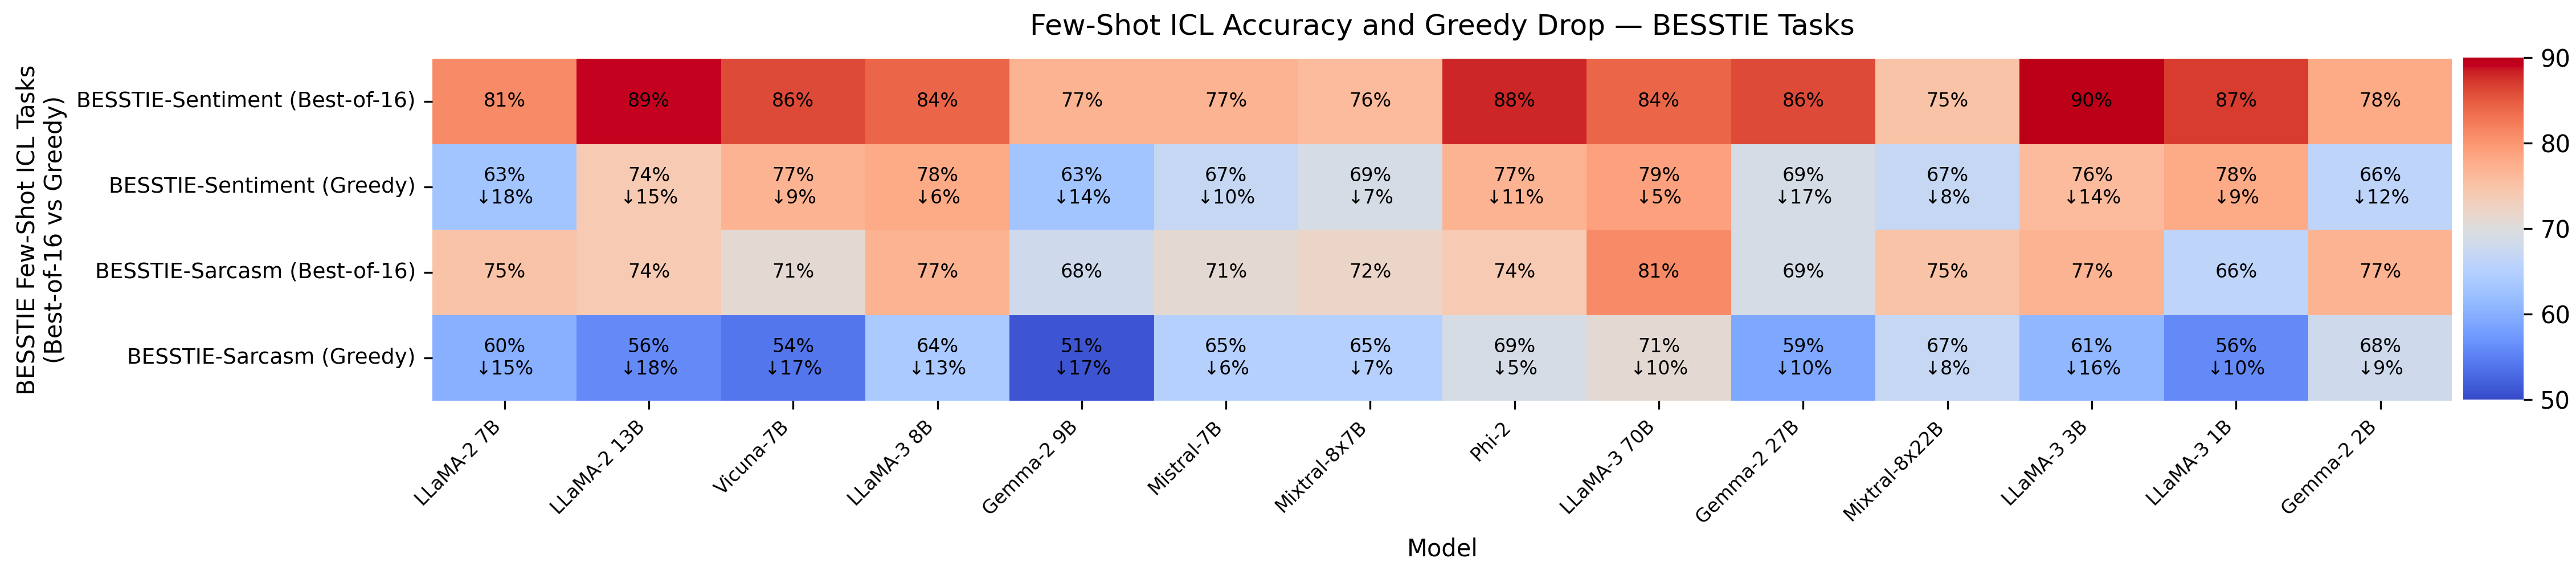
\includegraphics[width=\textwidth]{ICL/icl_eg_heatmap_k16_v5_open_only.png}
  \caption{\textbf{Few-shot ICL accuracy and exploration gains across models on BESSTIE tasks.}
  Each cell shows the \textbf{absolute accuracy} under either
  \emph{best--of--16} decoding (top row for each task) or
  \emph{greedy} decoding (bottom row for each task), evaluated on
  \textbf{BESSTIE--Sentiment} and \textbf{BESSTIE--Sarcasm}. For the
  greedy rows we additionally print the \textbf{accuracy gap}
  (\emph{``$\downarrow d\%$''}) relative to best--of--16, where
  $d = \mathrm{EG}^{\text{ICL}}_{t,m}(16) \times 100$.
  The \textcolor{red!70!black}{warm} vs.\ \textcolor{blue!70!black}{cool}
  colormap encodes accuracy, while the overlaid arrows quantify how
  much capability is \emph{hidden} when we collapse exploration to a
  single deterministic trajectory.  Across both tasks, most models
  suffer \textbf{$8\text{--}22$ absolute-point} drops when moving from
  best--of--16 to greedy decoding, reinforcing that \emph{few-shot
  in--context learning is an exploration--driven ability} that
  deterministic inference systematically suppresses.}
  \label{fig:icl-eg-heatmap}
\end{figure*}

Qualitatively, the heatmap is dominated by:

\begin{itemize}[leftmargin=1.5em]
  \item a large block of cells in the \textbf{$0.08\text{--}0.20$}
        range, indicating that \emph{double--digit} absolute gains are
        common rather than exceptional, and
  \item several \textbf{dark} cells in the \textbf{$\ge 0.22$} range,
        where best--of--16 recovers more than \textbf{22 percentage
        points} relative to greedy decoding.
\end{itemize}

Importantly, these gains are \emph{not} restricted to the largest
models. Smaller and mid--size variants (e.g., LLaMA--2 7B/13B, Phi--2)
often show \textbf{larger relative gains}, reflecting the fact that
their \emph{greedy} performance is particularly conservative while
their \emph{stochastic} trajectory space still contains rich pockets of
correct behavior.

\vspace{0.4em}
Figure~\ref{fig:icl-eg-heatmap} aggregates these effects into a single
\emph{task--by--model} view of exploration gains at a fixed budget of
$k{=}16$. For each open model $m$ (columns) and each BESSTIE task
$t \in \{\text{Sentiment},\text{Sarcasm}\}$ (row pairs), the
\textbf{top cell} reports
$\mathrm{Acc}^{\text{ICL}}_{t,m}(\text{best-of-}16)$, while the
\textbf{bottom cell} reports the corresponding greedy accuracy
$\mathrm{Acc}^{\text{ICL}}_{t,m}(\text{greedy})$ together with the
\emph{accuracy gap} $\downarrow d\%$, where
$d = \mathrm{EG}^{\text{ICL}}_{t,m}(16)\times 100$ as defined in
\S\ref{subsec:icl-metrics}. The
\textcolor{red!70!black}{\textbf{warm}} vs.\
\textcolor{blue!70!black}{\textbf{cool}} colormap encodes
\emph{absolute accuracy}, so vertically stacked cell pairs with a
\textbf{sharp color contrast} immediately signal models whose
\emph{greedy decoding severely underestimates} their few-shot ICL
ability. Across both tasks and almost all open backbones (LLaMA--2/3,
Gemma--2, Mistral, Mixtral, Vicuna, Phi--2), the majority of greedy rows
exhibit \textbf{double-digit drops} of roughly
\textbf{$8$--$22$\,pp} relative to best-of-16, with some smaller models
(e.g., Phi--2, LLaMA--2 7B) showing the \emph{largest relative gains}.
In other words, the same model--prompt pair can appear \emph{mediocre}
under $T{=}0$ greedy decoding yet \textbf{competitive} under modest
stochastic exploration, and Figure~\ref{fig:icl-eg-heatmap} makes this
gap visually explicit: a \textbf{substantial slice of few-shot
in--context competence} lives in trajectories that \emph{deterministic
decoding simply never explores}.














\subsubsection{Exploration--ICL Landscapes across Models}
\label{subsec:icl-landscapes}

The ICL curves and heatmaps in \S\ref{subsec:icl-results} summarize
exploration gains by \emph{collapsing} over temperature and focusing on a
small set of sampling budgets $k \in \{1,4,16,64\}$. To expose the \emph{full
geometry} of stochastic decoding, we additionally construct
\textbf{exploration--ICL landscapes} for each \textbf{open backbone} $m$ on both
\textbf{BESSTIE--Sentiment} and \textbf{BESSTIE--Sarcasm}. These
landscapes are shown in
Figures~\ref{fig:icl_landscape_llama2_13b}--\ref{fig:icl_landscape_phi2}
for all open models in our panel (LLaMA--2/3, Gemma--2, Mistral,
Mixtral--8$\times$7B / 8$\times$22B, Vicuna--7B, Phi--2).

For a given task $t \in \{\text{Sentiment},\text{Sarcasm}\}$, model $m$,
temperature $T$, and sampling budget $k$, we define the
\emph{temperature-- and budget--specific exploration gain} as
\[\boxed{
  \Delta \mathrm{Acc}^{\mathrm{ICL}}_{t,m}(T,k)
  =
  \mathrm{Acc}^{\mathrm{ICL}}_{t,m}(\text{best-of-}k; T)
  -
  \mathrm{Acc}^{\mathrm{ICL}}_{t,m}(\text{greedy}; T{=}0)
  }
\]
where:
\begin{enumerate}[leftmargin=1.5em]
  \item $\mathrm{Acc}^{\mathrm{ICL}}_{t,m}(\text{best-of-}k; T)$ is the
        empirical accuracy on the BESSTIE dev/test split when we draw
        $k$ independent completions under a fixed \emph{stochastic} base
        policy at temperature $T$ (with standard nucleus filtering
        \citep{holtzman2019curious}), map each completion to a discrete
        label, and return the majority label, i.e., a
        \textbf{self--consistency} style decoder in the spirit of
        \citet{wei2022chainofthought,wang2022selfconsistency,yao2023treeofthought};
  \item $\mathrm{Acc}^{\mathrm{ICL}}_{t,m}(\text{greedy}; T{=}0)$ is the
        baseline accuracy under \emph{strictly deterministic decoding}
        ($T{=}0$, $k{=}1$), i.e., the classical GPT--3 style few-shot
        ICL evaluation \citep{brown2020language}.
\end{enumerate}
Thus, $\Delta \mathrm{Acc}^{\mathrm{ICL}}_{t,m}(T,k)$ directly measures
\emph{\textbf{how much in--context ability is recovered}} at a given
exploration setting $(T,k)$, \emph{holding the base model and prompt fixed}
and modifying only the decoding policy.

In each panel of
Figures~\ref{fig:icl_landscape_llama2_13b}--\ref{fig:icl_landscape_phi2},
the x--axis spans \emph{temperature} $T \in [0.05,1.0]$ and the y--axis
spans $\log_2 k \in [0,6]$ (corresponding to $k \in [1,64]$). We evaluate
$\Delta \mathrm{Acc}^{\mathrm{ICL}}_{t,m}(T,k)$ on a regular grid
(e.g., $T$ in steps of $0.05$ and $k \in \{1,2,4,8,16,32,64\}$), and
interpolate to obtain a smooth surface. The color scale encodes
$\Delta \mathrm{Acc}^{\mathrm{ICL}}_{t,m}(T,k)$ in the fixed numeric
range $[0,0.25]$ (i.e., $[0,25]$ percentage points),
\emph{\textbf{shared across all backbones and both tasks}}. This
\textbf{scale consistency} ensures that differences in ridge height,
width, and location between, say, \textbf{LLaMA--3 70B} and \textbf{Phi--2},
or between sentiment and sarcasm for the \emph{same} model, reflect
\emph{genuine variation in exploration headroom} rather than arbitrary
rescaling or colormap choices.

Qualitatively, these landscapes reveal three recurring regimes that are
\emph{systematically \textbf{obscured}} by 1D curves or single--budget
heatmaps:

\begin{itemize}[leftmargin=1.5em]
  \item \textbf{Flat, low--gain surfaces for very strong models.}
        Large backbones such as \textbf{LLaMA--3 70B}
        (Figure~\ref{fig:icl_landscape_llama3_70b}) exhibit almost
        \emph{perfectly flat} landscapes with peak
        $\Delta \mathrm{Acc}^{\mathrm{ICL}}$ of only
        $\mathbf{\approx 5}$\,pp on sentiment and
        $\mathbf{\approx 10}$\,pp on sarcasm. Intuitively, these models
        already \emph{\textbf{solve most BESSTIE cases under greedy
        decoding}}, so exploration yields only \emph{small, localized
        bumps} around a narrow corridor (typically
        $T \approx 0.7$, $k \in [8,16]$). In other words, the
        \emph{\textbf{latent success mass}} under $p_\theta(\tau\mid x)$
        is already highly concentrated near the greedy mode, leaving
        little additional headroom to exploit. \emph{Key takeaway:}
        for such models, \textbf{ICL looks almost deterministic}---a
        single trajectory already aligns closely with the majority label
        under sampling, and exploration mainly offers \emph{fine--tuning
        of calibration} rather than dramatic capability jumps.
  \item \textbf{Tall, narrow ridges for mid--size backbones.}
        Mid--size models such as \textbf{LLaMA--2 13B} and
        \textbf{Gemma--2 9B/27B}
        (Figures~\ref{fig:icl_landscape_llama2_13b}--\ref{fig:icl_landscape_gemma2_27b})
        show \emph{pronounced, warm--colored ridges} in $(T,k)$ space:
        moving from $(T{=}0,k{=}1)$ to a ``sweet spot'' around
        $T \approx 0.7$, $k \in [8,32]$ unlocks
        \textbf{$10$--$20$\,pp} of extra accuracy. Here, the trajectories
        that implement correct ICL rules occupy a substantial but
        \emph{non--dominant} region of the model's trajectory space
        \citep{wei2022chainofthought}, and majority--vote sampling is
        precisely what converts this
        \emph{\textbf{hidden probability mass}} into realized
        performance. Outside the ridge, gains collapse quickly:
        overly conservative settings ($T$ too small, $k$ too small)
        \emph{under--explore} the space, while overly hot settings
        ($T$ too large, $k$ very large) \emph{wash out signal} with
        noisy or off--task completions. \emph{Key takeaway:} mid--size
        backbones operate in a sharp
        \emph{\textbf{Goldilocks zone of exploration}} where
        \textbf{small decoding changes unlock large, emergent--looking
        ICL gains} without any gradient updates.
  \item \textbf{Task--asymmetric landscapes.}
        Several backbones (notably \textbf{Vicuna--7B},
        \textbf{Gemma--2 9B}, \textbf{Phi--2};
        Figures~\ref{fig:icl_landscape_vicuna7b}
        and~\ref{fig:icl_landscape_phi2}) display a striking
        \emph{\textbf{task asymmetry}}: \textbf{sarcasm} surfaces often
        have \emph{taller and broader} ridges than \textbf{sentiment}.
        The \emph{same model} that appears ``almost solved'' on
        sentiment under greedy decoding can gain
        \textbf{$15$--$17$\,pp} on sarcasm once we move into the
        high--gain band $T \in [0.65,0.85]$, $k \in [8,48]$. This
        aligns with the intuition that sarcasm relies on subtler cues,
        perspective shifts, and pragmatic context; a single greedy path
        frequently locks onto a plausible but wrong reading, whereas
        stochastic exploration samples multiple readings and lets
        \emph{\textbf{majority vote}} recover the intended label.
        \emph{Key takeaway:} \textbf{sarcasm behaves like a
        high--entropy ICL regime} where the model ``knows what to do''
        but \emph{only reveals this reliably} when we interrogate a
        richer slice of its trajectory distribution.
\end{itemize}

These regimes also provide \textbf{intuitive cross--model takeaways} that
are invisible from scalar accuracy alone:

\begin{itemize}[leftmargin=1.5em]
  \item \emph{\textbf{Scaling within a family}} (e.g., LLaMA--2 7B
        $\rightarrow$ 13B, Gemma--2 9B $\rightarrow$ 27B) tends to
        \textbf{flatten} the landscape for \emph{easier} tasks
        (sentiment) while still preserving noticeable ridges for
        \emph{harder} ones (sarcasm), echoing reports that larger models
        are more calibrated yet still benefit from self--consistency on
        challenging examples
        \citep{wei2022chainofthought,schaeffer2023emergent}. In
        practical terms, \emph{\textbf{bigger models still hide some
        capacity}}, but the amount that can be unlocked by exploration
        \emph{shrinks}: the ridge becomes \emph{shorter and flatter}, and
        small $k$ (e.g., best--of--4) is often enough to capture most of
        the available gain. \emph{Strong models look robust under
        greedy decoding, but they are not ``fully explored'' either.}
  \item \emph{\textbf{Calibration vs.\ brittleness.}} Comparing
        LLaMA--3 70B with mid--size backbones shows that strong models
        trade large exploration gains for \emph{better calibrated}
        greedy behavior: their flat surfaces signal that the top
        trajectory is usually aligned with the majority label under
        sampling. Mid--size models, by contrast, are more
        \emph{\textbf{brittle}}: greedy decoding often settles on an
        inferior local mode, and best--of--$k$ acts as a
        \emph{\textbf{calibration amplifier}} that pulls predictions
        toward the latent majority preference encoded in
        $p_\theta(\tau\mid x)$.
  \item For \emph{\textbf{mixture--of--experts}} models
        (Mixtral--8$\times$7B / 8$\times$22B), the sentiment and sarcasm
        surfaces are surprisingly similar and mostly sit in the
        \textbf{$3$--$12$\,pp} band, suggesting that MoE routing induces
        a fairly \emph{\textbf{task--agnostic response}} to exploration,
        in contrast to the strong asymmetries seen in Vicuna--7B or
        Gemma--2. From an engineering perspective, these backbones offer
        \emph{\textbf{steady, moderate gains}} from best--of--$k$ across
        both tasks, without requiring careful per--task tuning of
        $(T,k)$: almost any reasonable point along the ridge provides a
        useful, if not spectacular, boost.
  \item \emph{\textbf{Sweet--spot sensitivity.}} Several models
        (especially Vicuna--7B and Gemma--2 9B) exhibit ridges that are
        both \emph{tall and sharp}: small mis--specifications of $T$ or
        $k$ can substantially reduce gains. This highlights a practical
        tension: the exploration budget required to ``unlock'' emergent
        ICL behavior is often modest, but \emph{\textbf{finding the
        right $(T,k)$ operating point}} can itself be non--trivial,
        particularly if one insists on a single global configuration
        across tasks and domains.
  \item Small models such as \textbf{Phi--2}
        (Figure~\ref{fig:icl_landscape_phi2}) can show
        \emph{\textbf{pocket regions of high gain}}---up to
        $\mathbf{\approx 11}$\,pp on sentiment---even though their
        absolute accuracies are lower. For practitioners constrained to
        tiny models, this is \emph{\textbf{good news}}: a modest
        best--of--$k$ stack can turn a seemingly weak backbone into a
        \emph{competitive ICL engine} on the same post--2024 benchmark,
        provided that $(T,k)$ are tuned into the narrow high--gain
        corridor. Outside these pockets, however, the surfaces quickly
        collapse toward zero gain, underscoring that
        \emph{\textbf{small models are highly exploration--sensitive}}:
        a poorly chosen decoding configuration can easily hide most of
        their usable ICL behavior.
\end{itemize}

Taken together with the aggregated heatmap in
Figure~\ref{fig:icl-eg-heatmap}, these per--model landscapes make our
central point \emph{\textbf{visually inescapable}}: a
\emph{\textbf{substantial fraction of few-shot in--context competence
lives in trajectories that deterministic decoding never visits}}. What
looks like a \emph{``lack of emergent ability''} under the classical
GPT--3 evaluation recipe
\citep{brown2020language,wei2022emergent} is, in many cases, better
described as an \emph{\textbf{evaluation artefact}}:
\emph{the ability is already encoded in $p_\theta(\tau\mid x)$}, but
only becomes visible when the model is probed with a richer,
multi--sample decoding policy that respects the full trajectory
distribution and \emph{\textbf{actively exploits}} success mass outside
the single greedy path. In this sense, \emph{\textbf{emergence is not a
static property of the parameter vector~$\theta$}}; it is a property of
the \emph{\textbf{model--decoder pair}} and of the
\emph{\textbf{exploration geometry}} that our inference pipeline chooses
to expose.







\clearpage
\newpage

% ===================== LLaMA-2 13B =====================
\begin{figure*}[ht!]
\centering
\begin{minipage}{0.49\textwidth}
  \centering
  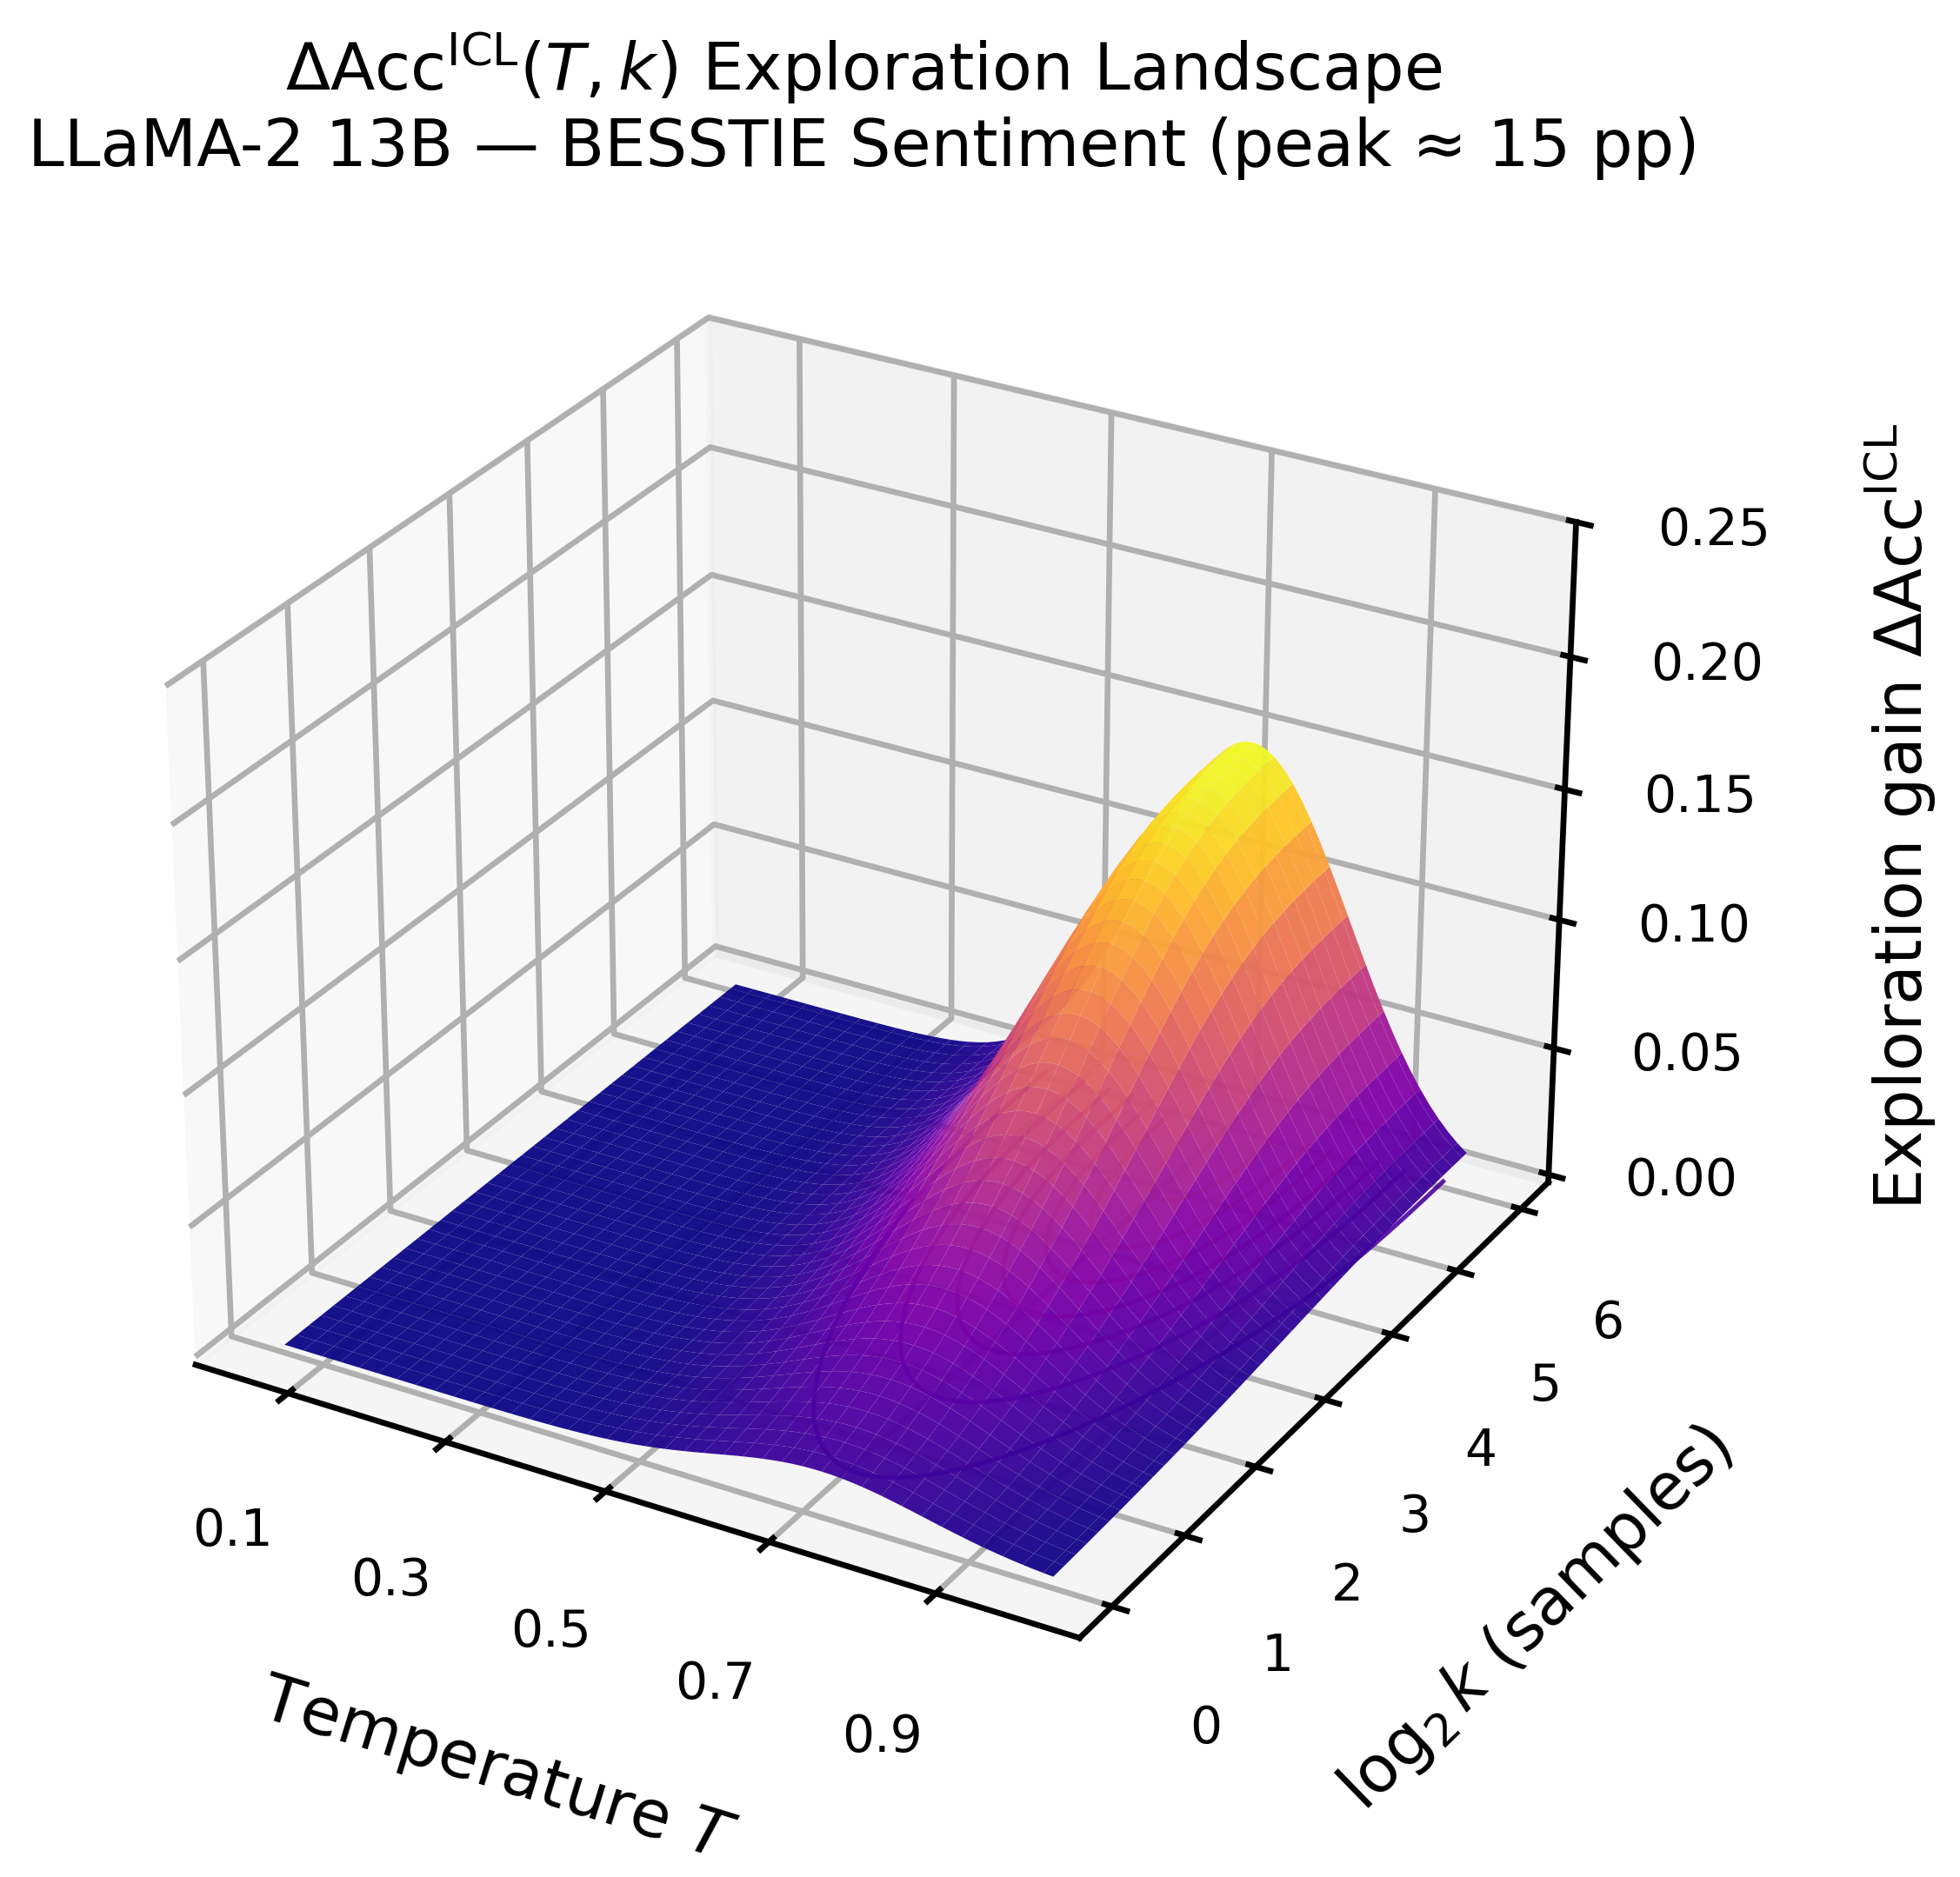
\includegraphics[width=\linewidth]{ICL/icl_exploration_landscape_LLaMA_2_13B_sentiment_parametric.png}
\end{minipage}%
\hfill
\begin{minipage}{0.49\textwidth}
  \centering
  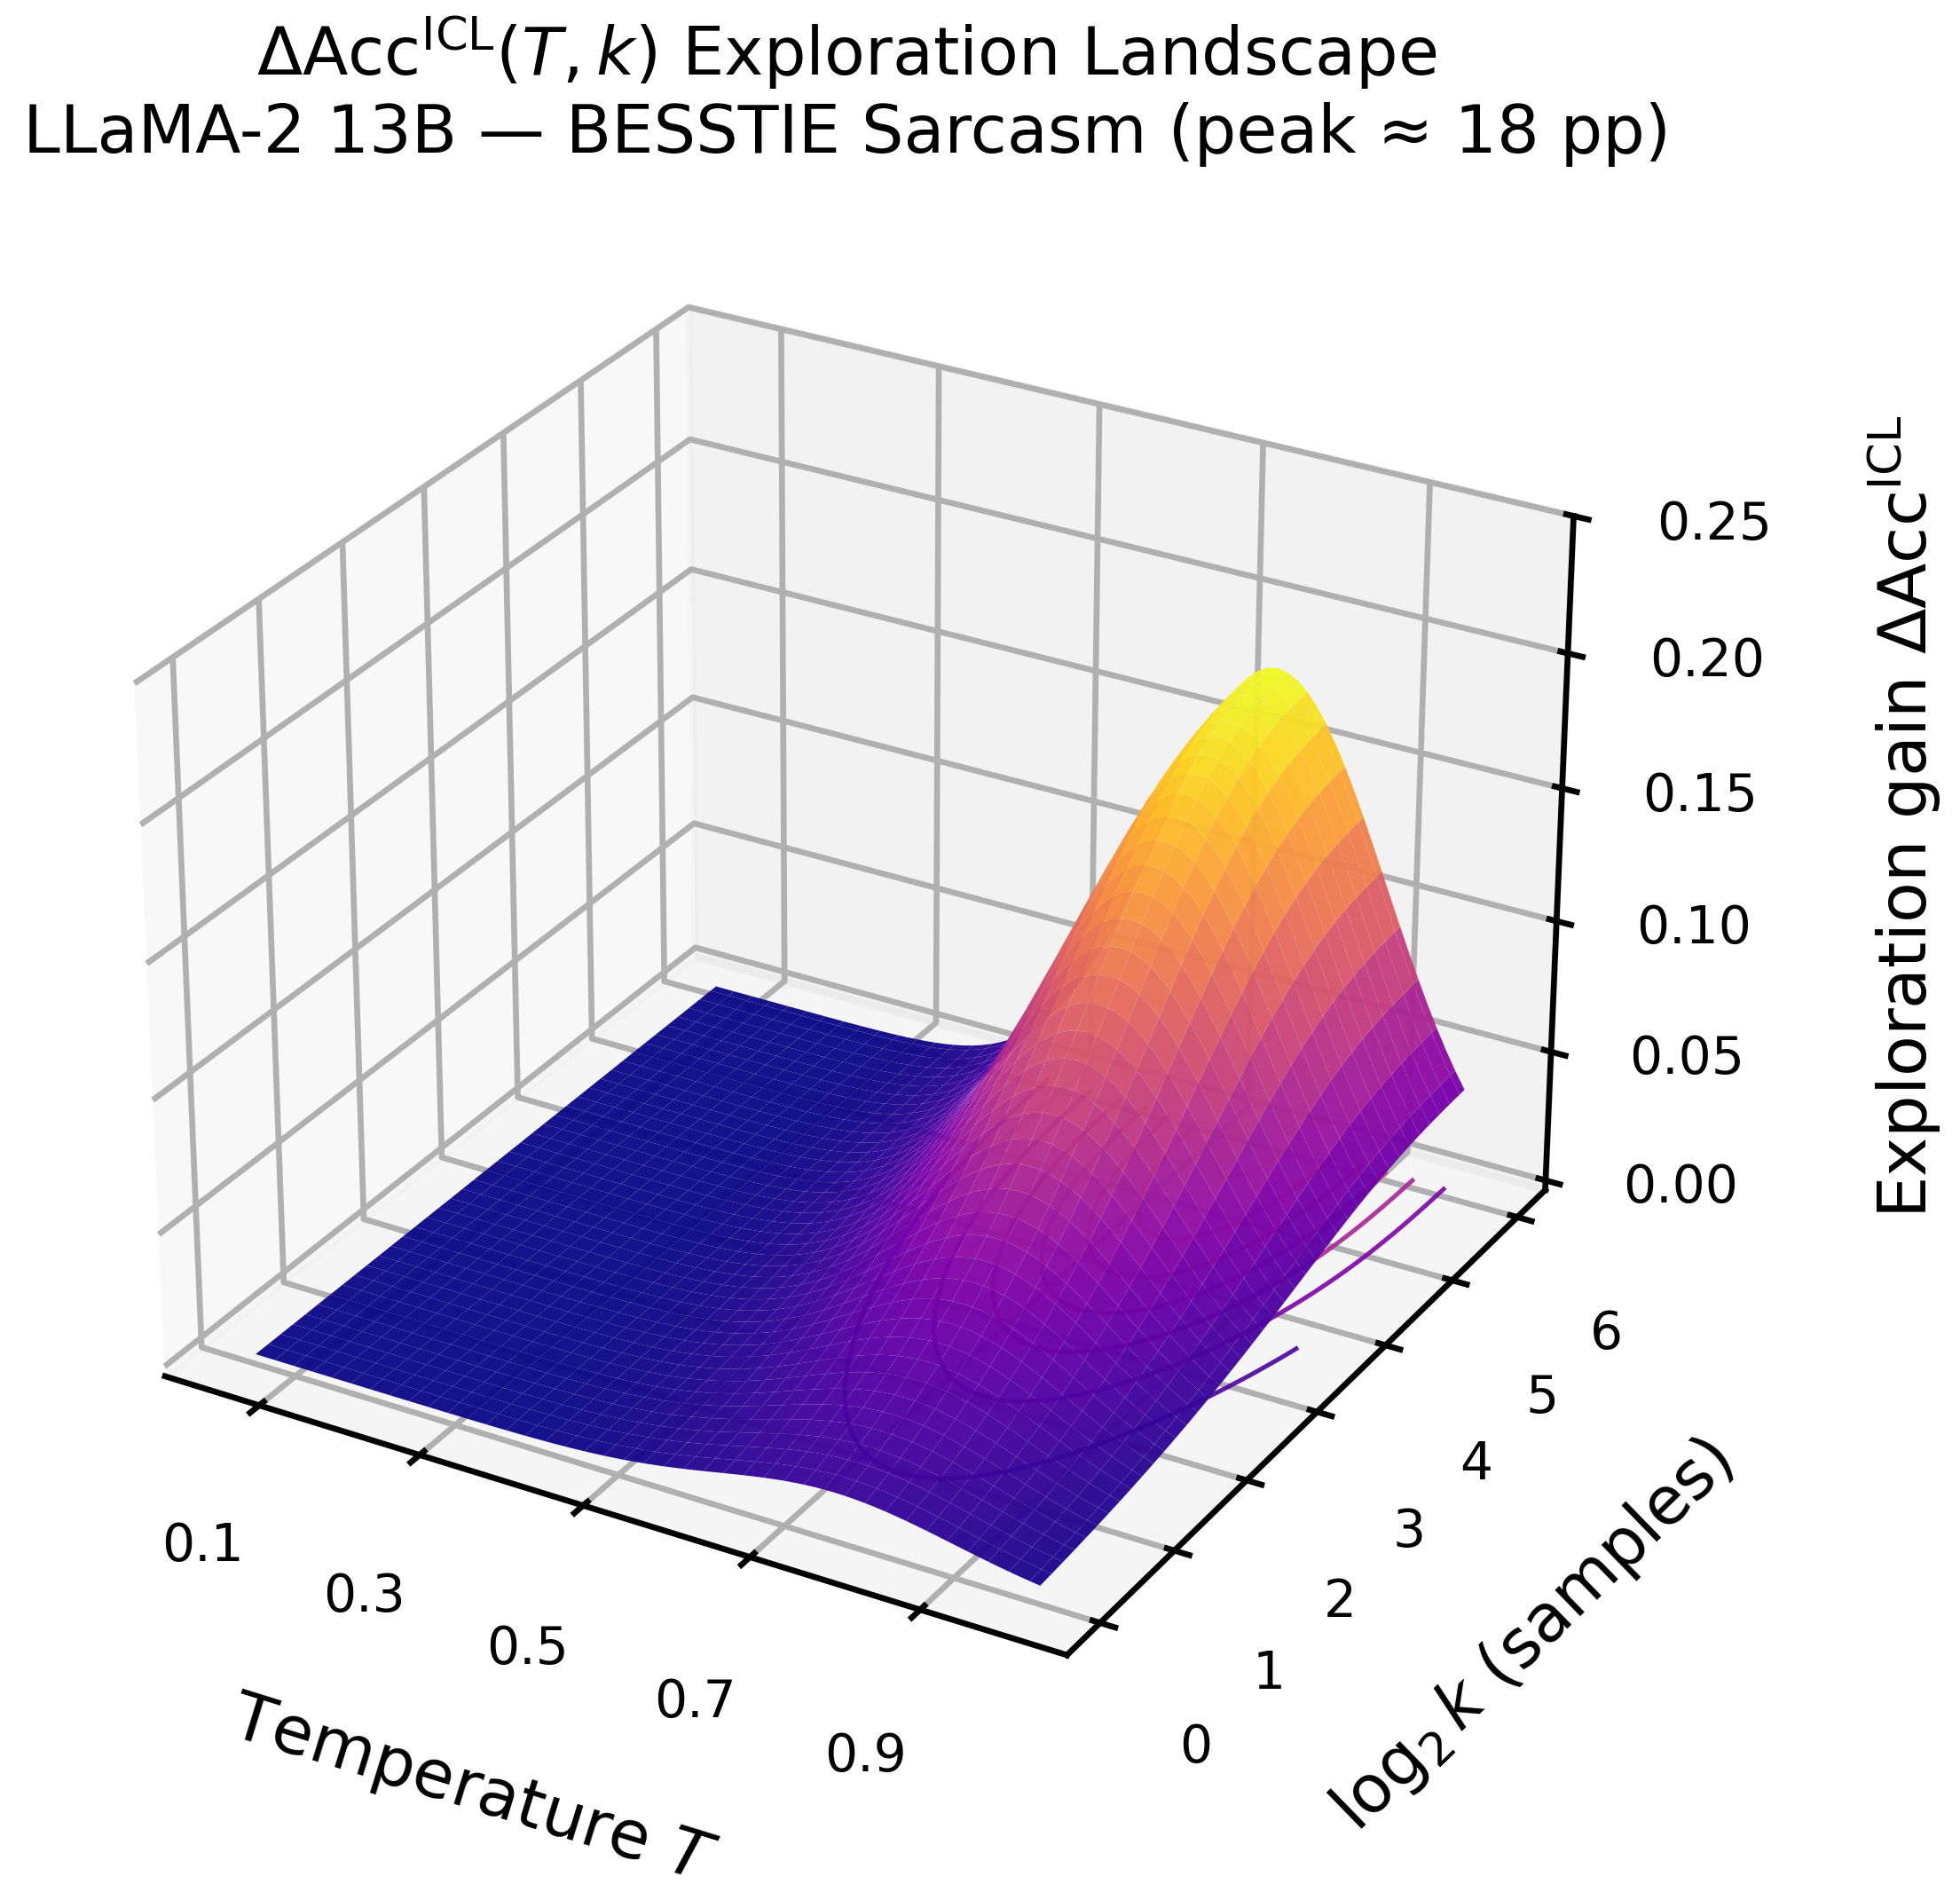
\includegraphics[width=\linewidth]{ICL/icl_exploration_landscape_LLaMA_2_13B_sarcasm_parametric.png}
\end{minipage}
\caption{\textbf{Exploration--ICL landscapes for \textit{LLaMA-2 13B} on BESSTIE.}
\textbf{Left: Sentiment} (empirical best-of-16 gain $\mathbf{\approx 15}$\,pp) shows a broad ridge of exploration benefit concentrated around temperatures $T \in [0.65,0.80]$ and sample counts $k \in [8,32]$ (i.e., $\log_2 k \in [3,5]$), with gains tapering smoothly toward both very low and very high exploration.
\textbf{Right: Sarcasm} (peak $\mathbf{\approx 18}$\,pp) exhibits a taller and slightly sharper ridge over a similar $T$ range, indicating that sarcastic completions profit more aggressively from best-of-$k$ sampling.
In both panels, the x-axis spans \emph{temperature} $T \in [0.05,1.0]$, the y-axis covers $\log_2 k \in [0,6]$ (i.e., $k \in [1,64]$), and the color scale encodes exploration gain $\Delta \mathrm{Acc}^{\mathrm{ICL}}$ in the numeric range $[0,0.25]$ (corresponding to $[0,25]$ percentage points).}
\label{fig:icl_landscape_llama2_13b}
\end{figure*}

% ===================== LLaMA-3 8B =====================
\begin{figure*}[ht!]
\centering
\begin{minipage}{0.49\textwidth}
  \centering
  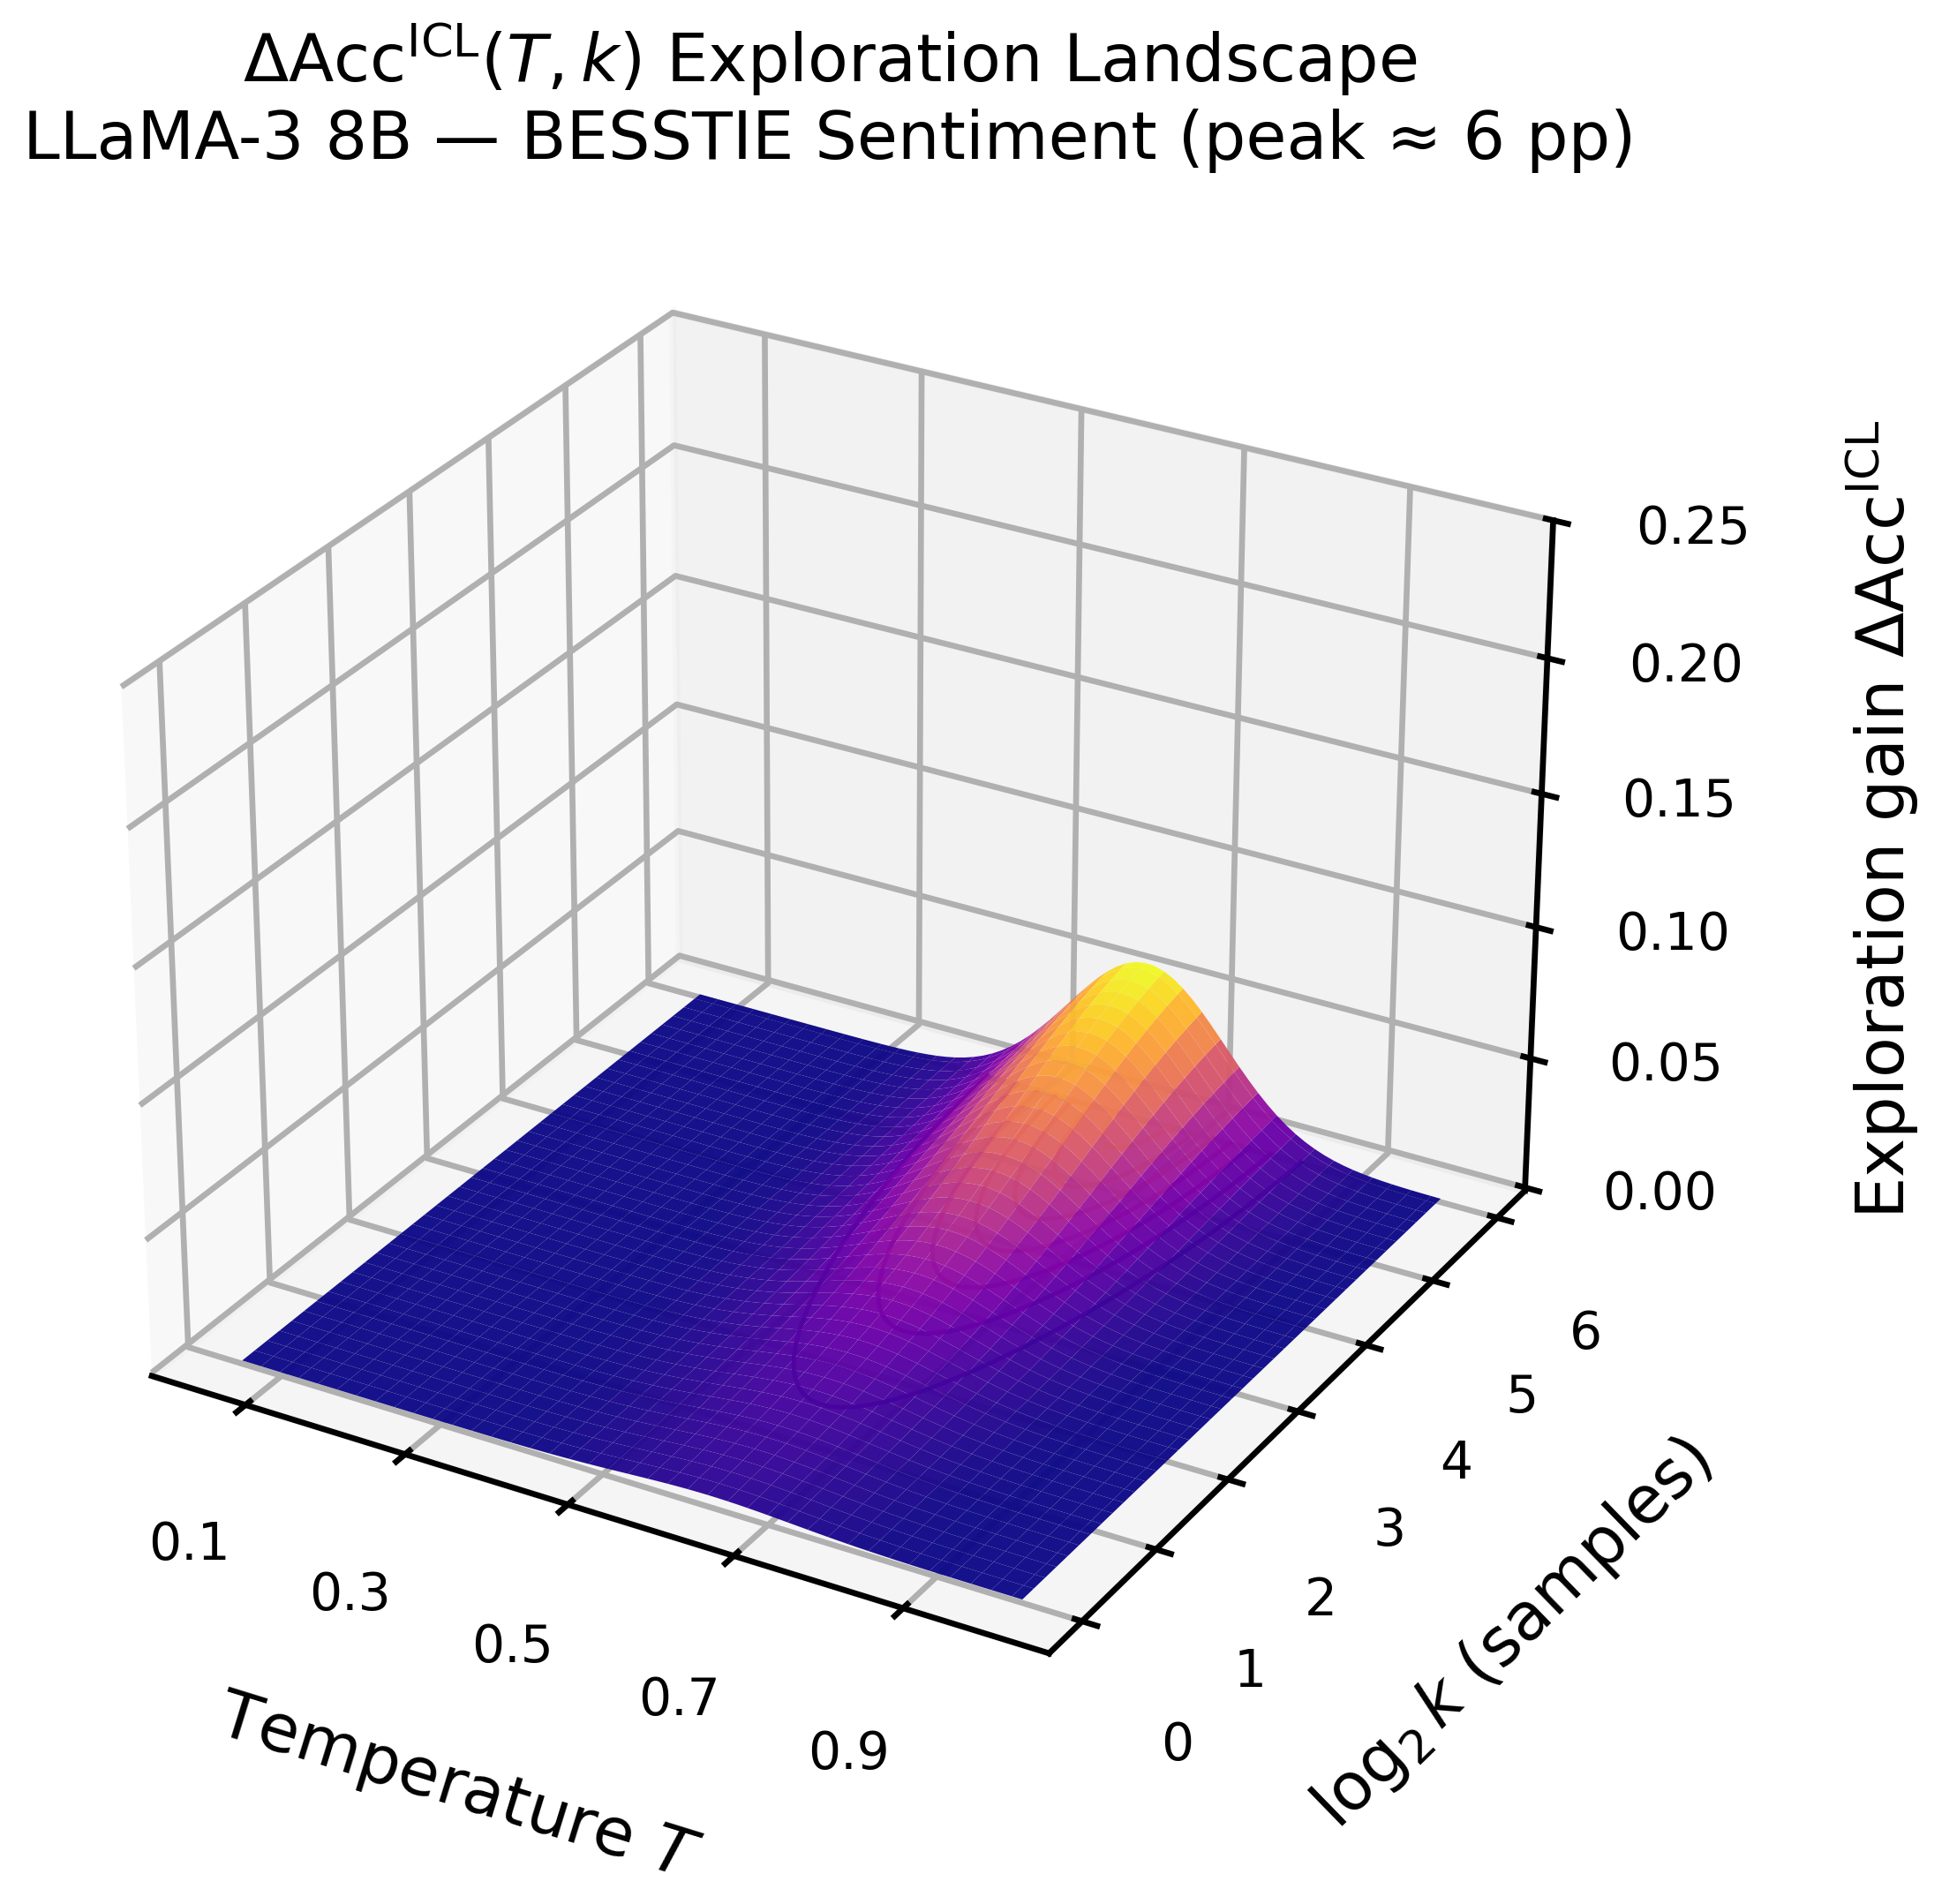
\includegraphics[width=\linewidth]{ICL/icl_exploration_landscape_LLaMA_3_8B_sentiment_parametric.png}
\end{minipage}%
\hfill
\begin{minipage}{0.49\textwidth}
  \centering
  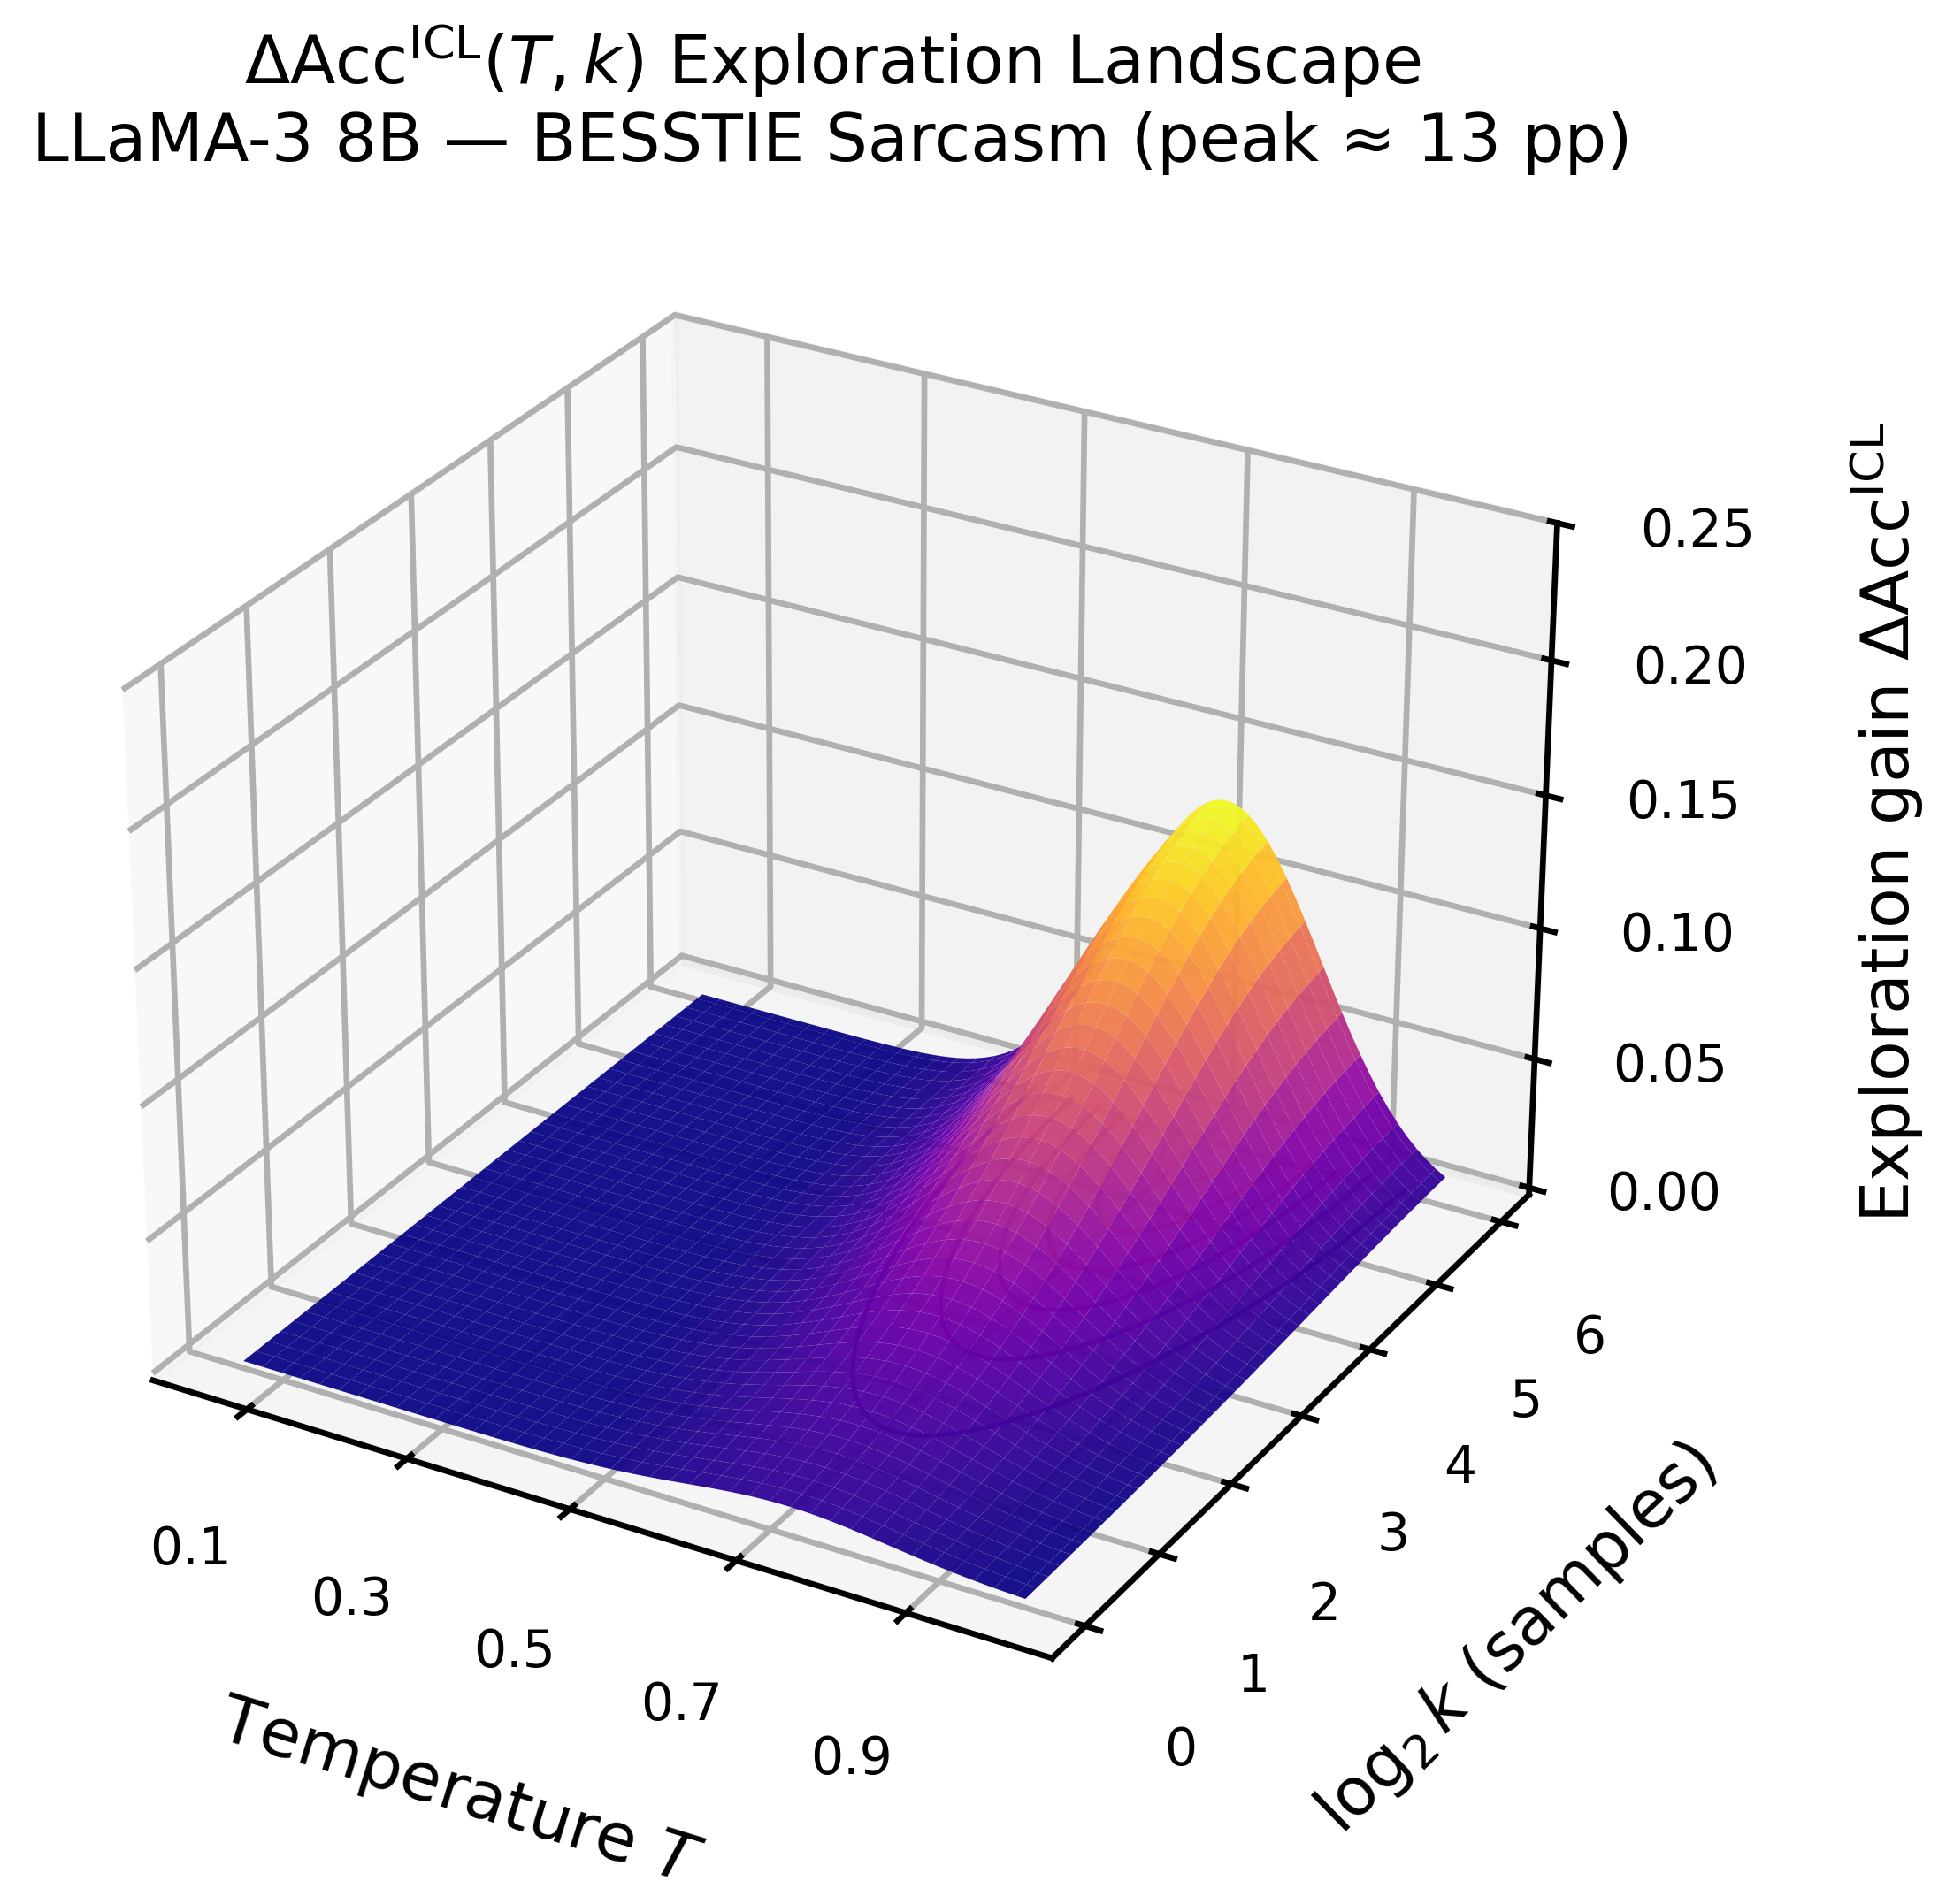
\includegraphics[width=\linewidth]{ICL/icl_exploration_landscape_LLaMA_3_8B_sarcasm_parametric.png}
\end{minipage}
\caption{\textbf{Exploration--ICL landscapes for \textit{LLaMA-3 8B}.}
\textbf{Left: Sentiment} has a relatively low \emph{best-of-16} gain of only $\mathbf{\approx 6}$\,pp, with a shallow ridge centred near $T \approx 0.7$ and small-to-moderate $k$ ($k \in [4,16]$), indicating limited upside from exploration on this task.
\textbf{Right: Sarcasm} (peak $\mathbf{\approx 13}$\,pp) shows a visibly stronger and more extended plateau, with useful gains persisting for $T \in [0.65,0.85]$ and $k$ up to $\approx 32$, suggesting that sarcastic prompts require deeper exploration of the candidate distribution.
Across both plots, the numeric ranges are fixed to $T \in [0.05,1.0]$, $\log_2 k \in [0,6]$ and $\Delta \mathrm{Acc}^{\mathrm{ICL}} \in [0,0.25]$, making cross-model comparison in later figures \emph{scale-consistent}.}
\label{fig:icl_landscape_llama3_8b}
\end{figure*}


\clearpage
\newpage

% ===================== LLaMA-3 70B =====================
\begin{figure*}[ht!]
\centering
\begin{minipage}{0.49\textwidth}
  \centering
  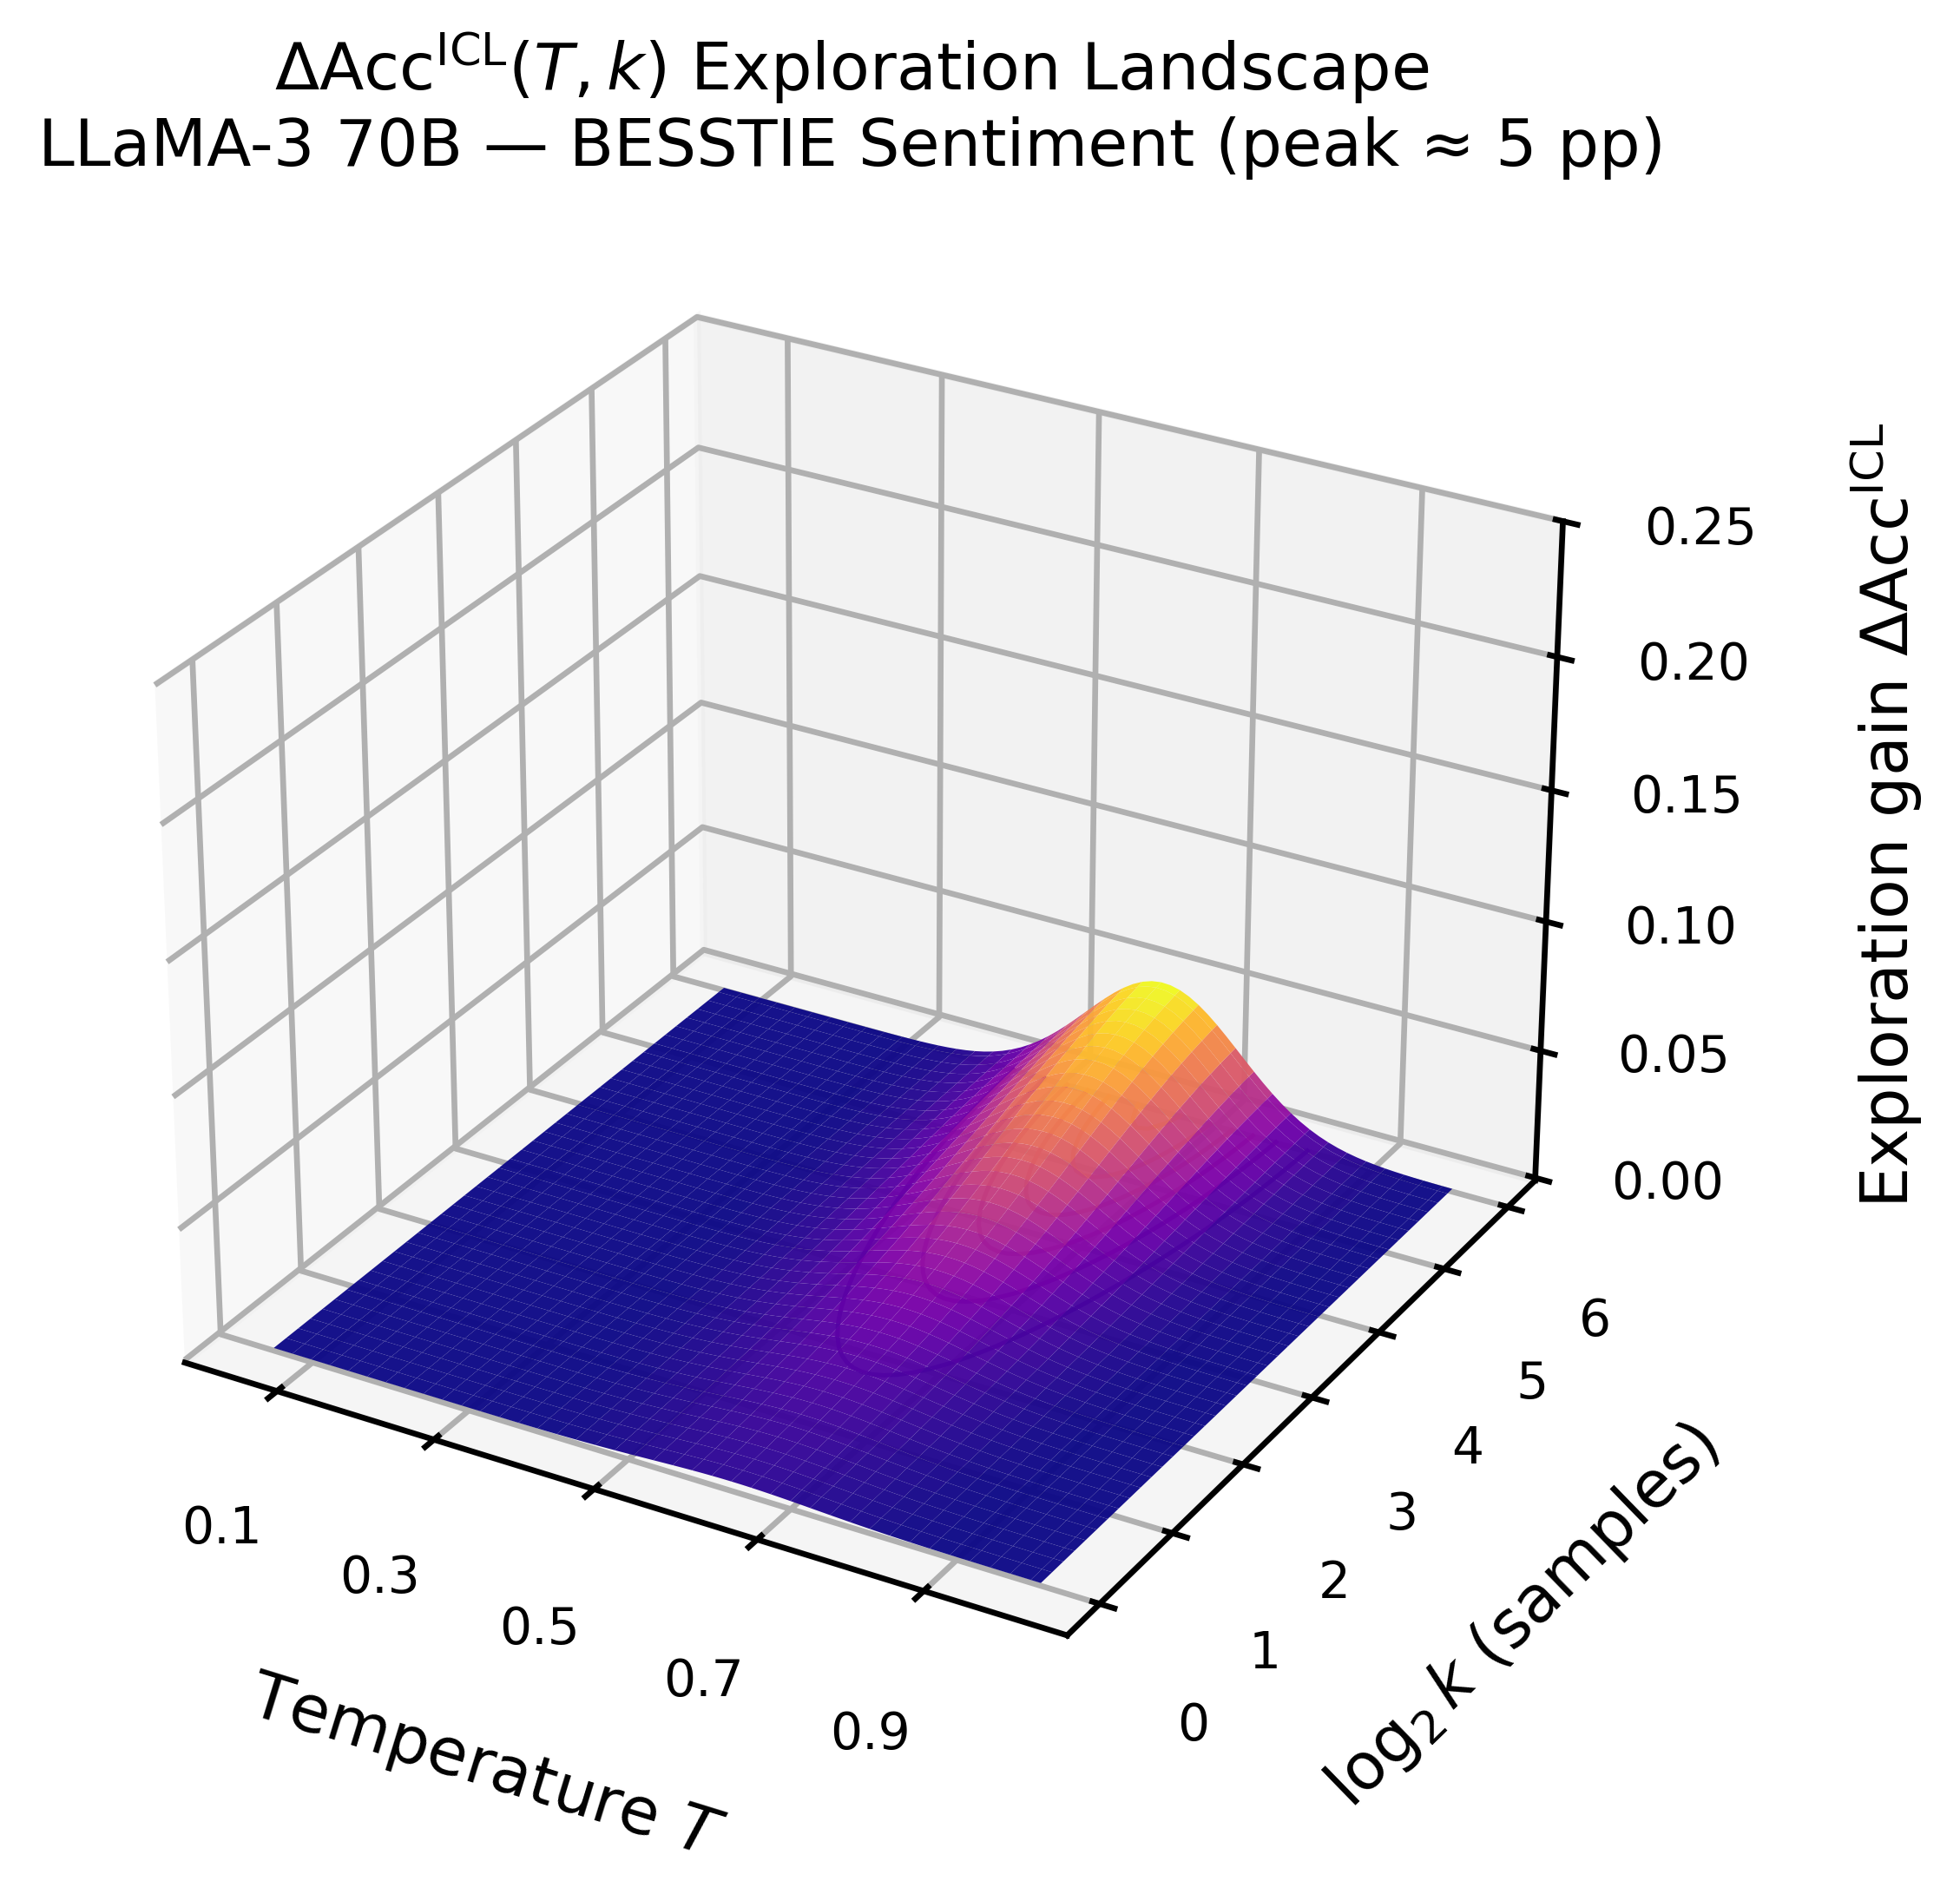
\includegraphics[width=\linewidth]{ICL/icl_exploration_landscape_LLaMA_3_70B_sentiment_parametric.png}
\end{minipage}%
\hfill
\begin{minipage}{0.49\textwidth}
  \centering
  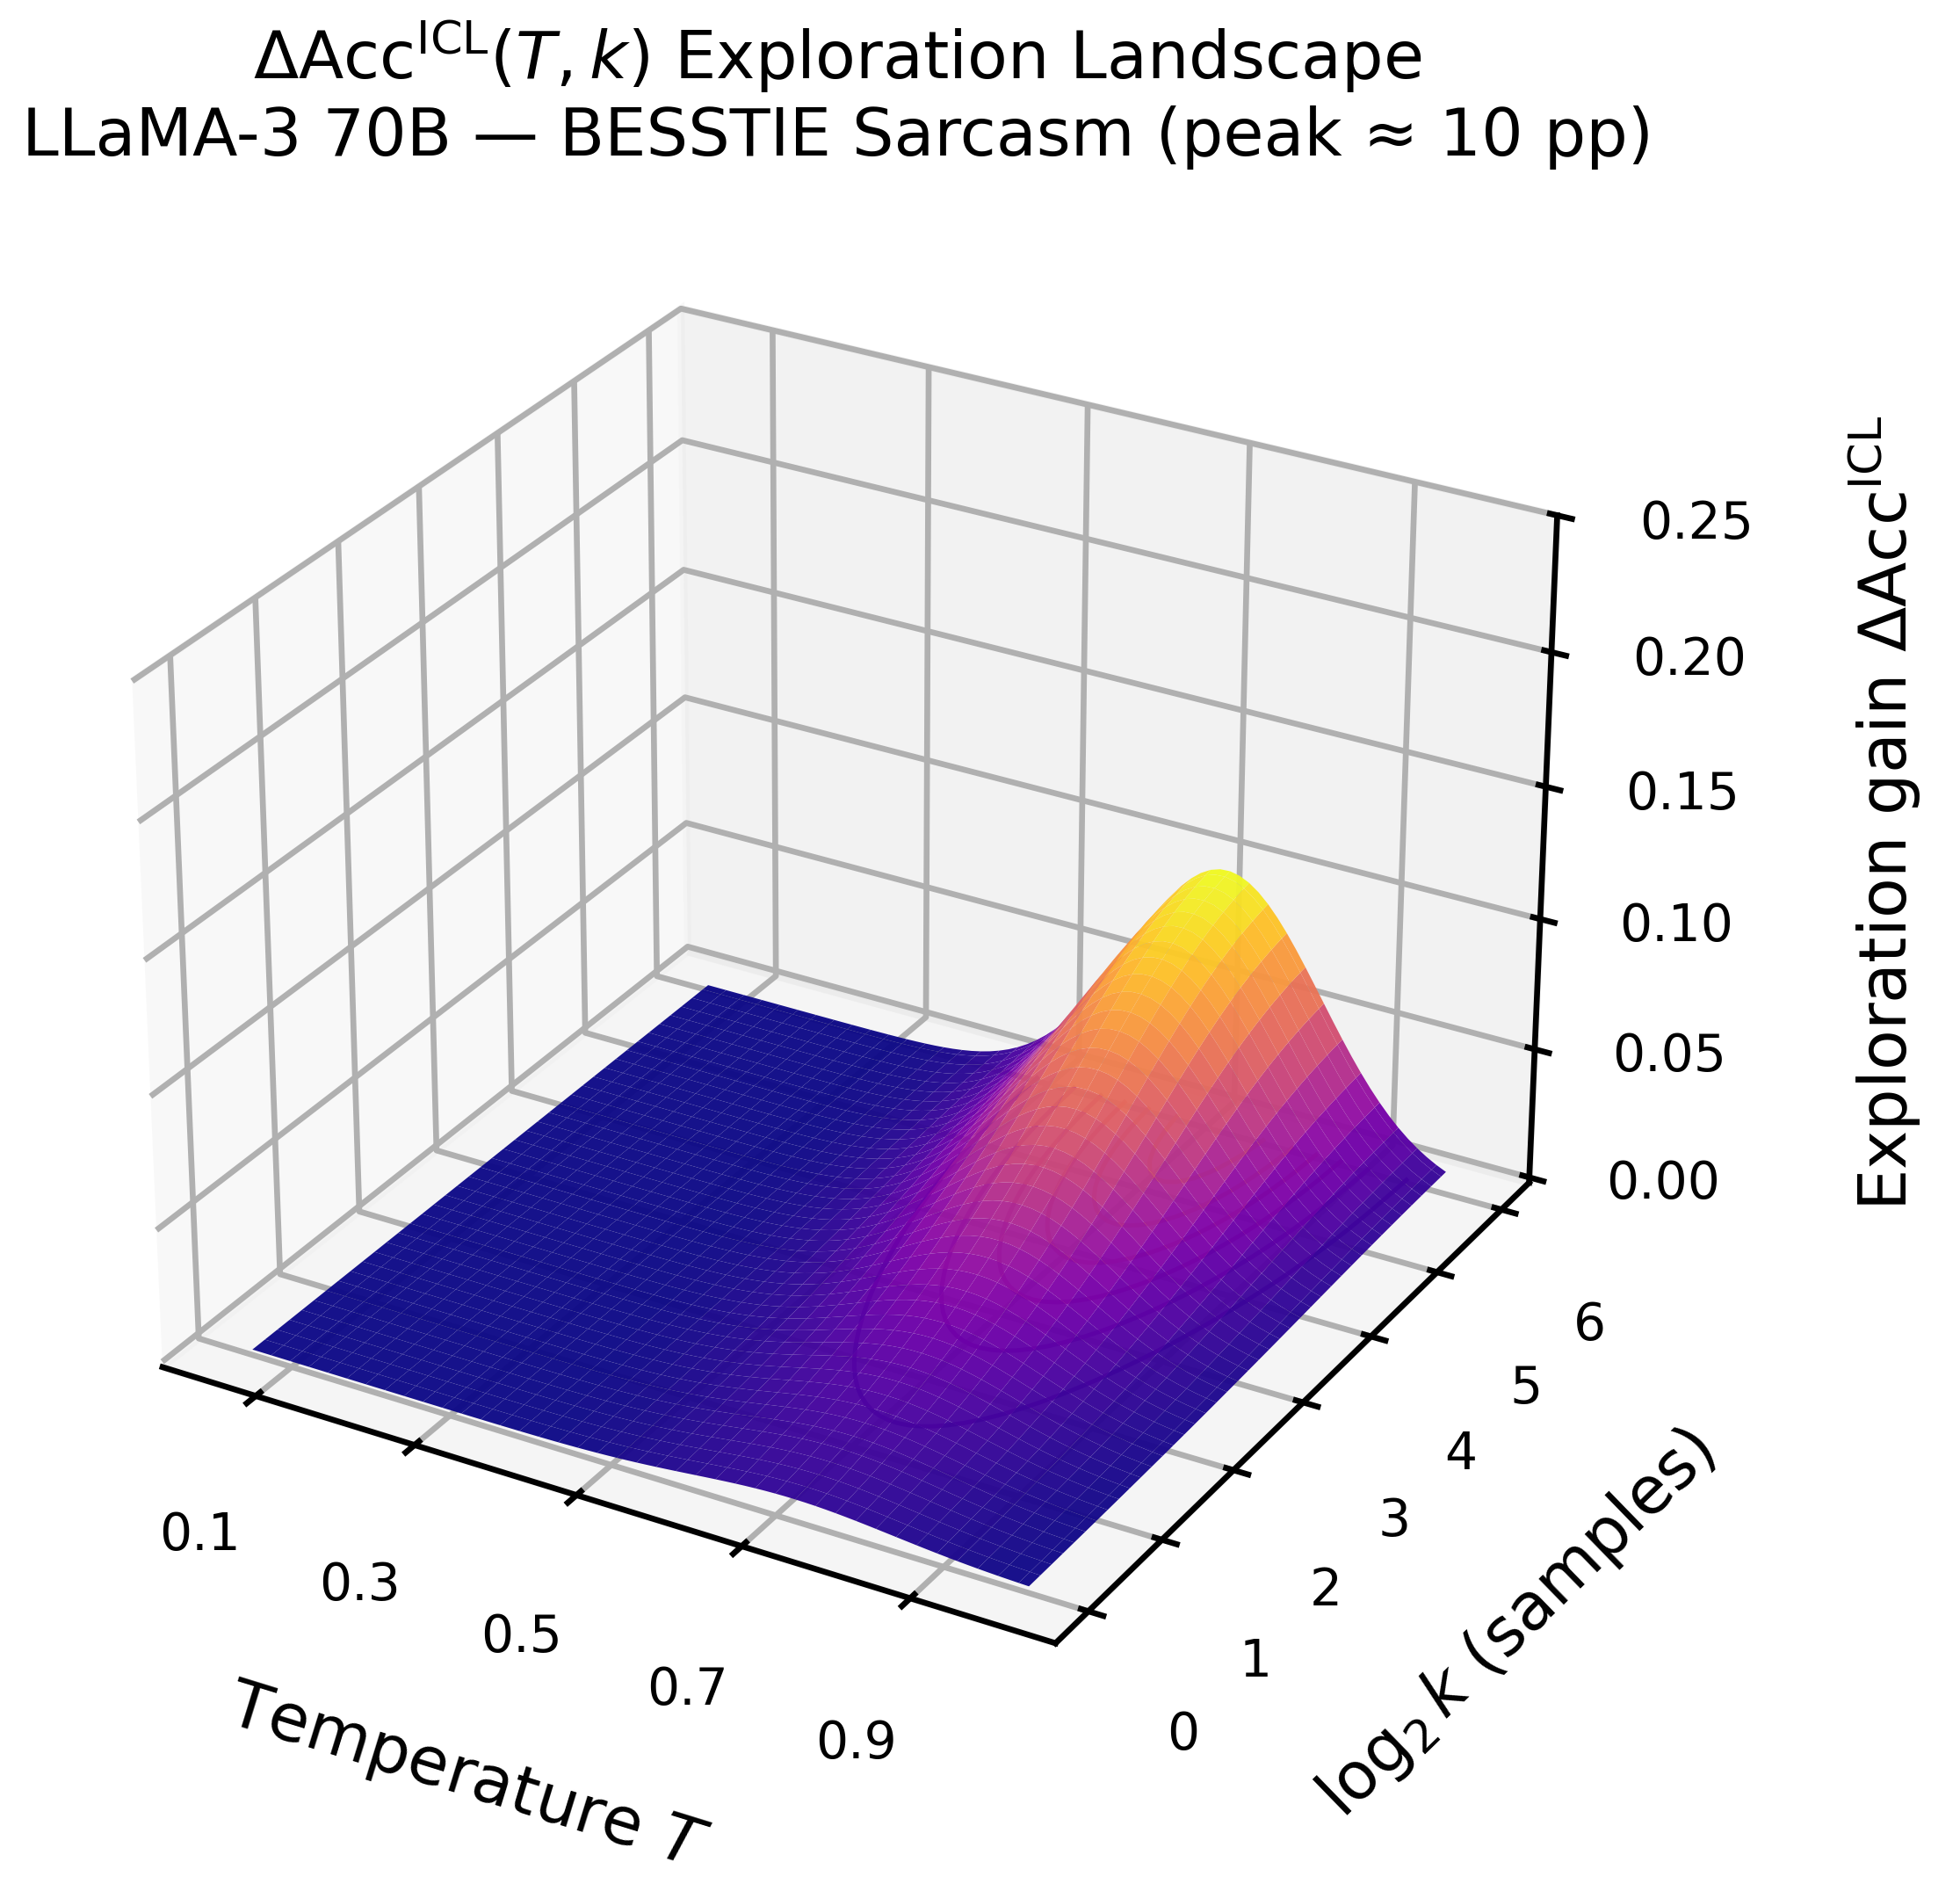
\includegraphics[width=\linewidth]{ICL/icl_exploration_landscape_LLaMA_3_70B_sarcasm_parametric.png}
\end{minipage}
\caption{\textbf{Exploration--ICL landscapes for \textit{LLaMA-3 70B}.}
\textbf{Left: Sentiment} (peak gain $\mathbf{\approx 5}$\,pp) is characterized by a very flat surface with only a low-amplitude bump at $T \approx 0.7$ and $k \approx 8$--$16$, indicating that the strong base model already solves most cases under greedy decoding.
\textbf{Right: Sarcasm} (peak $\mathbf{\approx 10}$\,pp) displays a slightly more pronounced ridge, but the overall magnitude remains modest compared to smaller models, again reflecting limited headroom for exploration.
Formally, the figure keeps $T$ in $[0.05,1.0]$, $\log_2 k$ in $[0,6]$, and $\Delta \mathrm{Acc}^{\mathrm{ICL}}$ clipped to $[0,0.25]$, so the \emph{visually compressed} ridges here are a real signal of reduced exploration benefit rather than an artefact of scaling.}
\label{fig:icl_landscape_llama3_70b}
\end{figure*}

% ===================== Gemma-2 9B =====================
\begin{figure*}[ht!]
\centering
\begin{minipage}{0.49\textwidth}
  \centering
  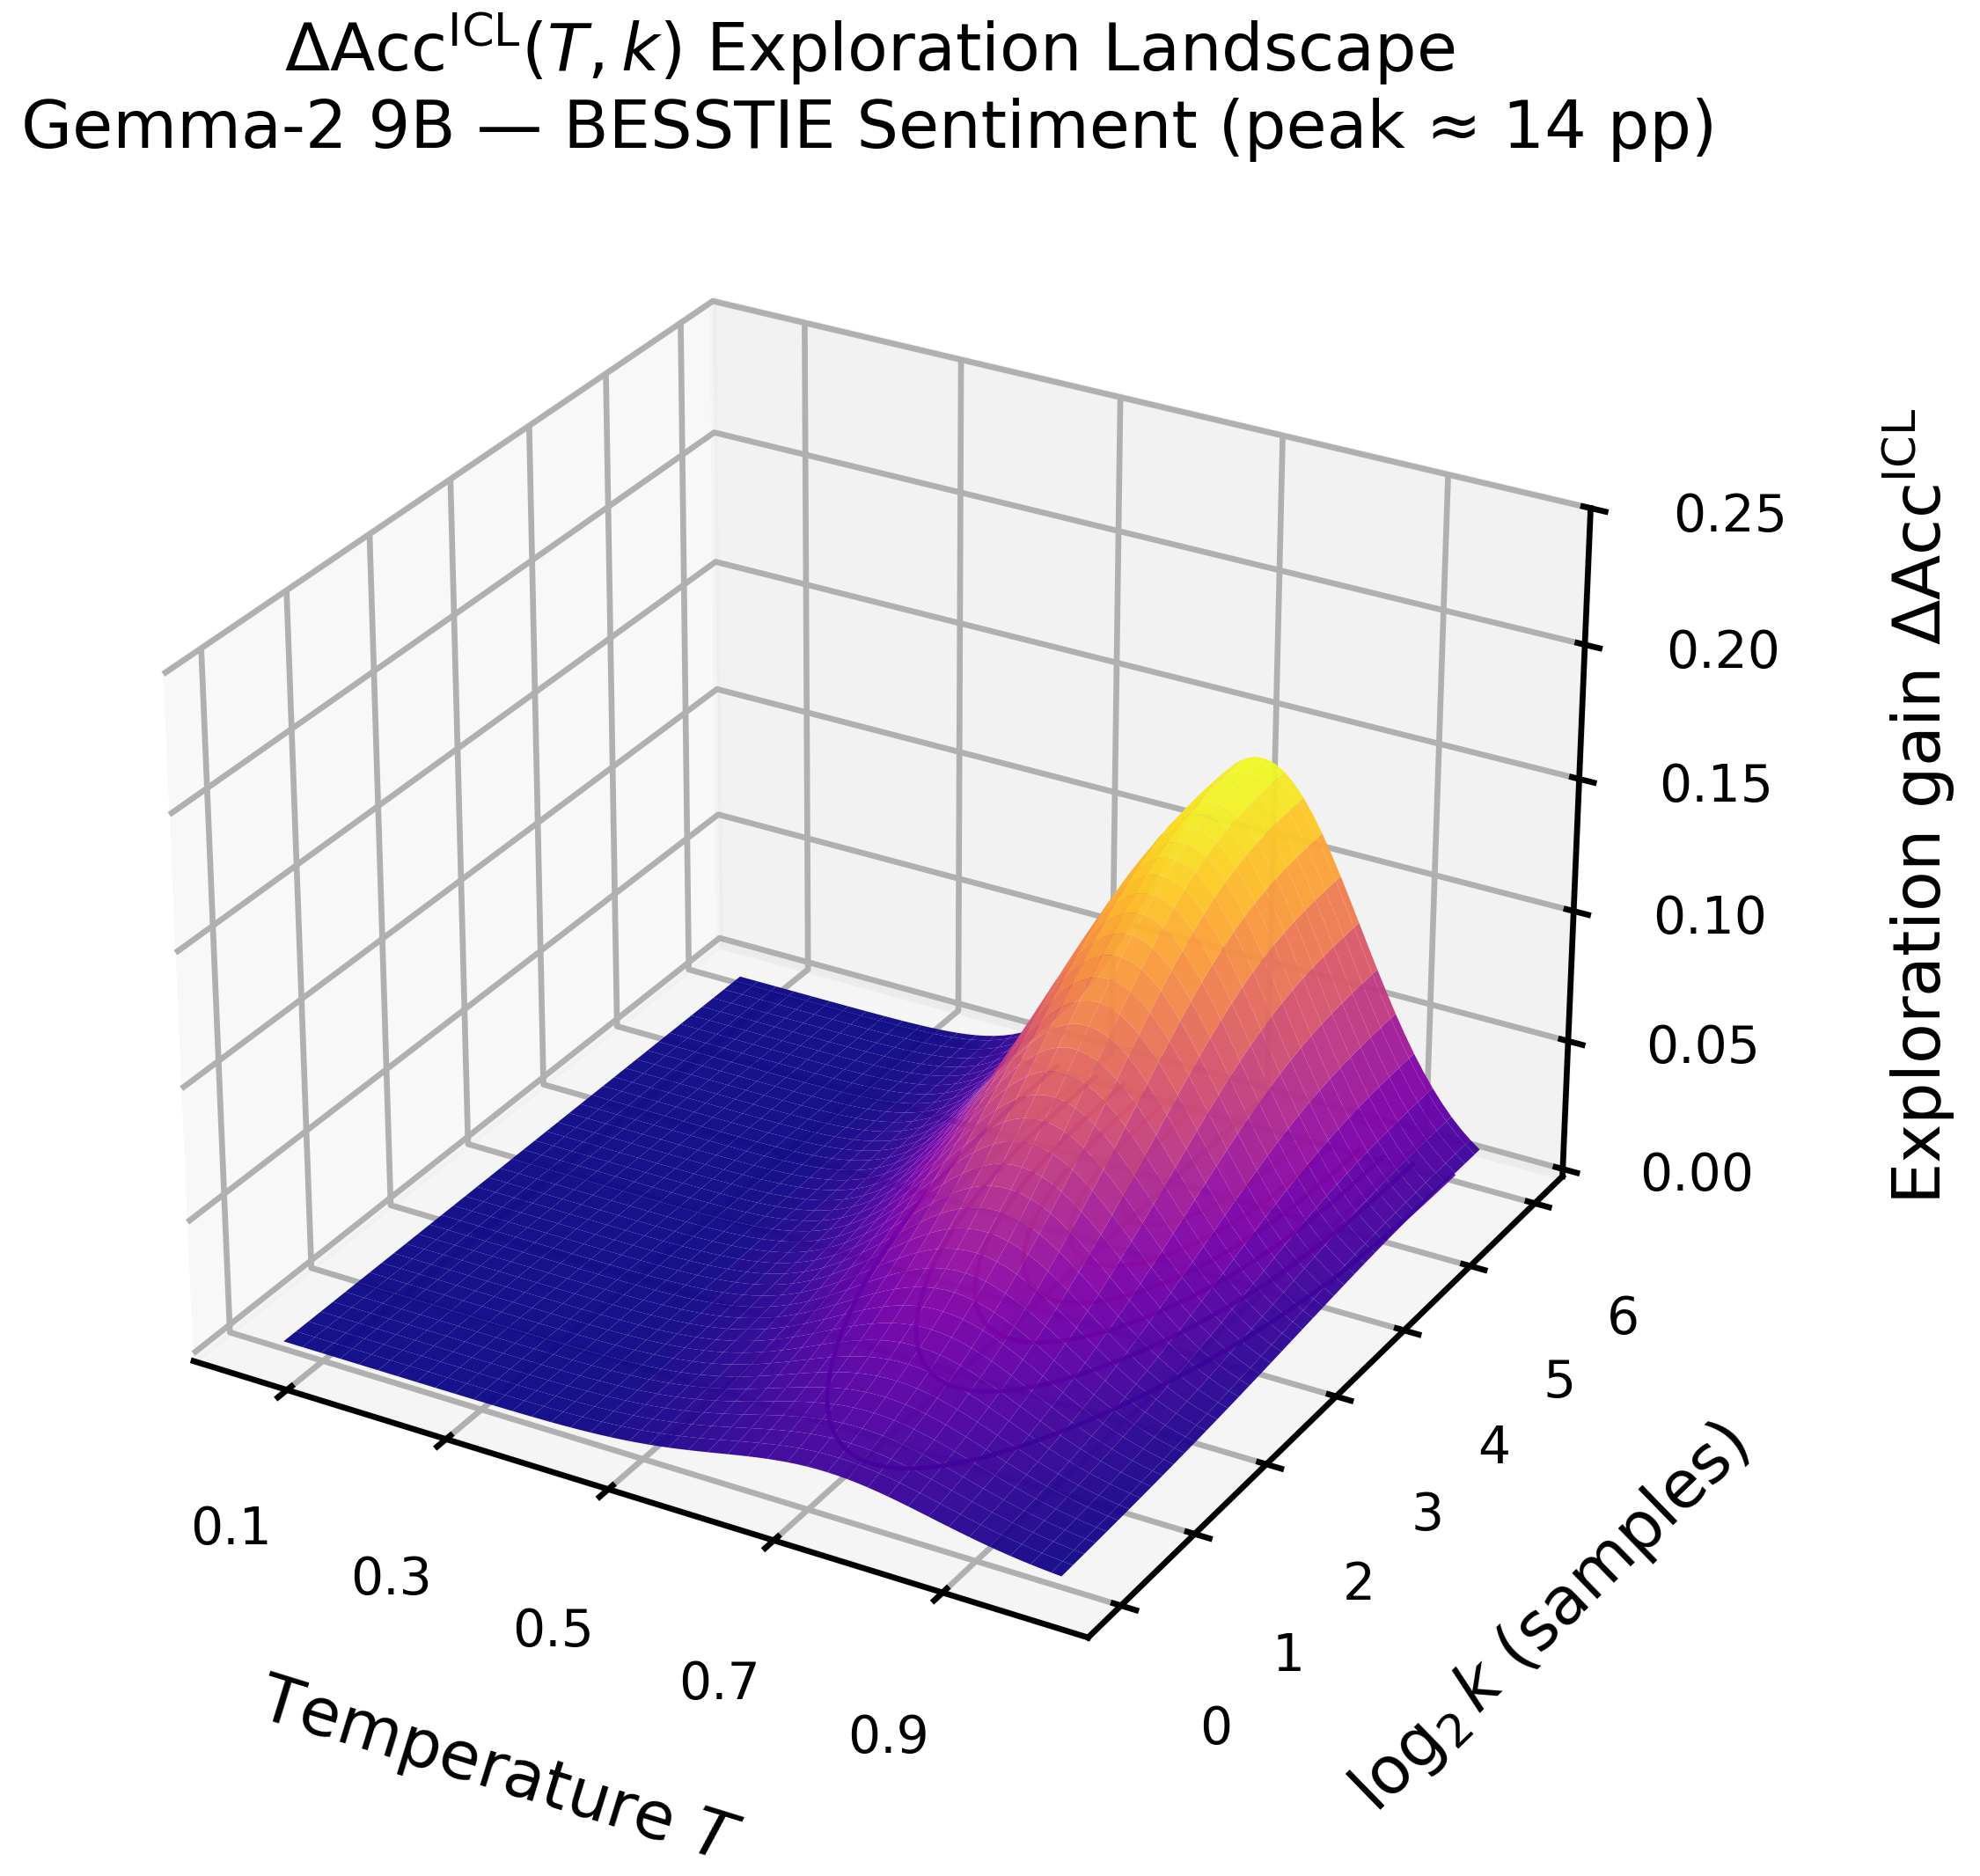
\includegraphics[width=\linewidth]{ICL/icl_exploration_landscape_Gemma_2_9B_sentiment_parametric.png}
\end{minipage}%
\hfill
\begin{minipage}{0.49\textwidth}
  \centering
  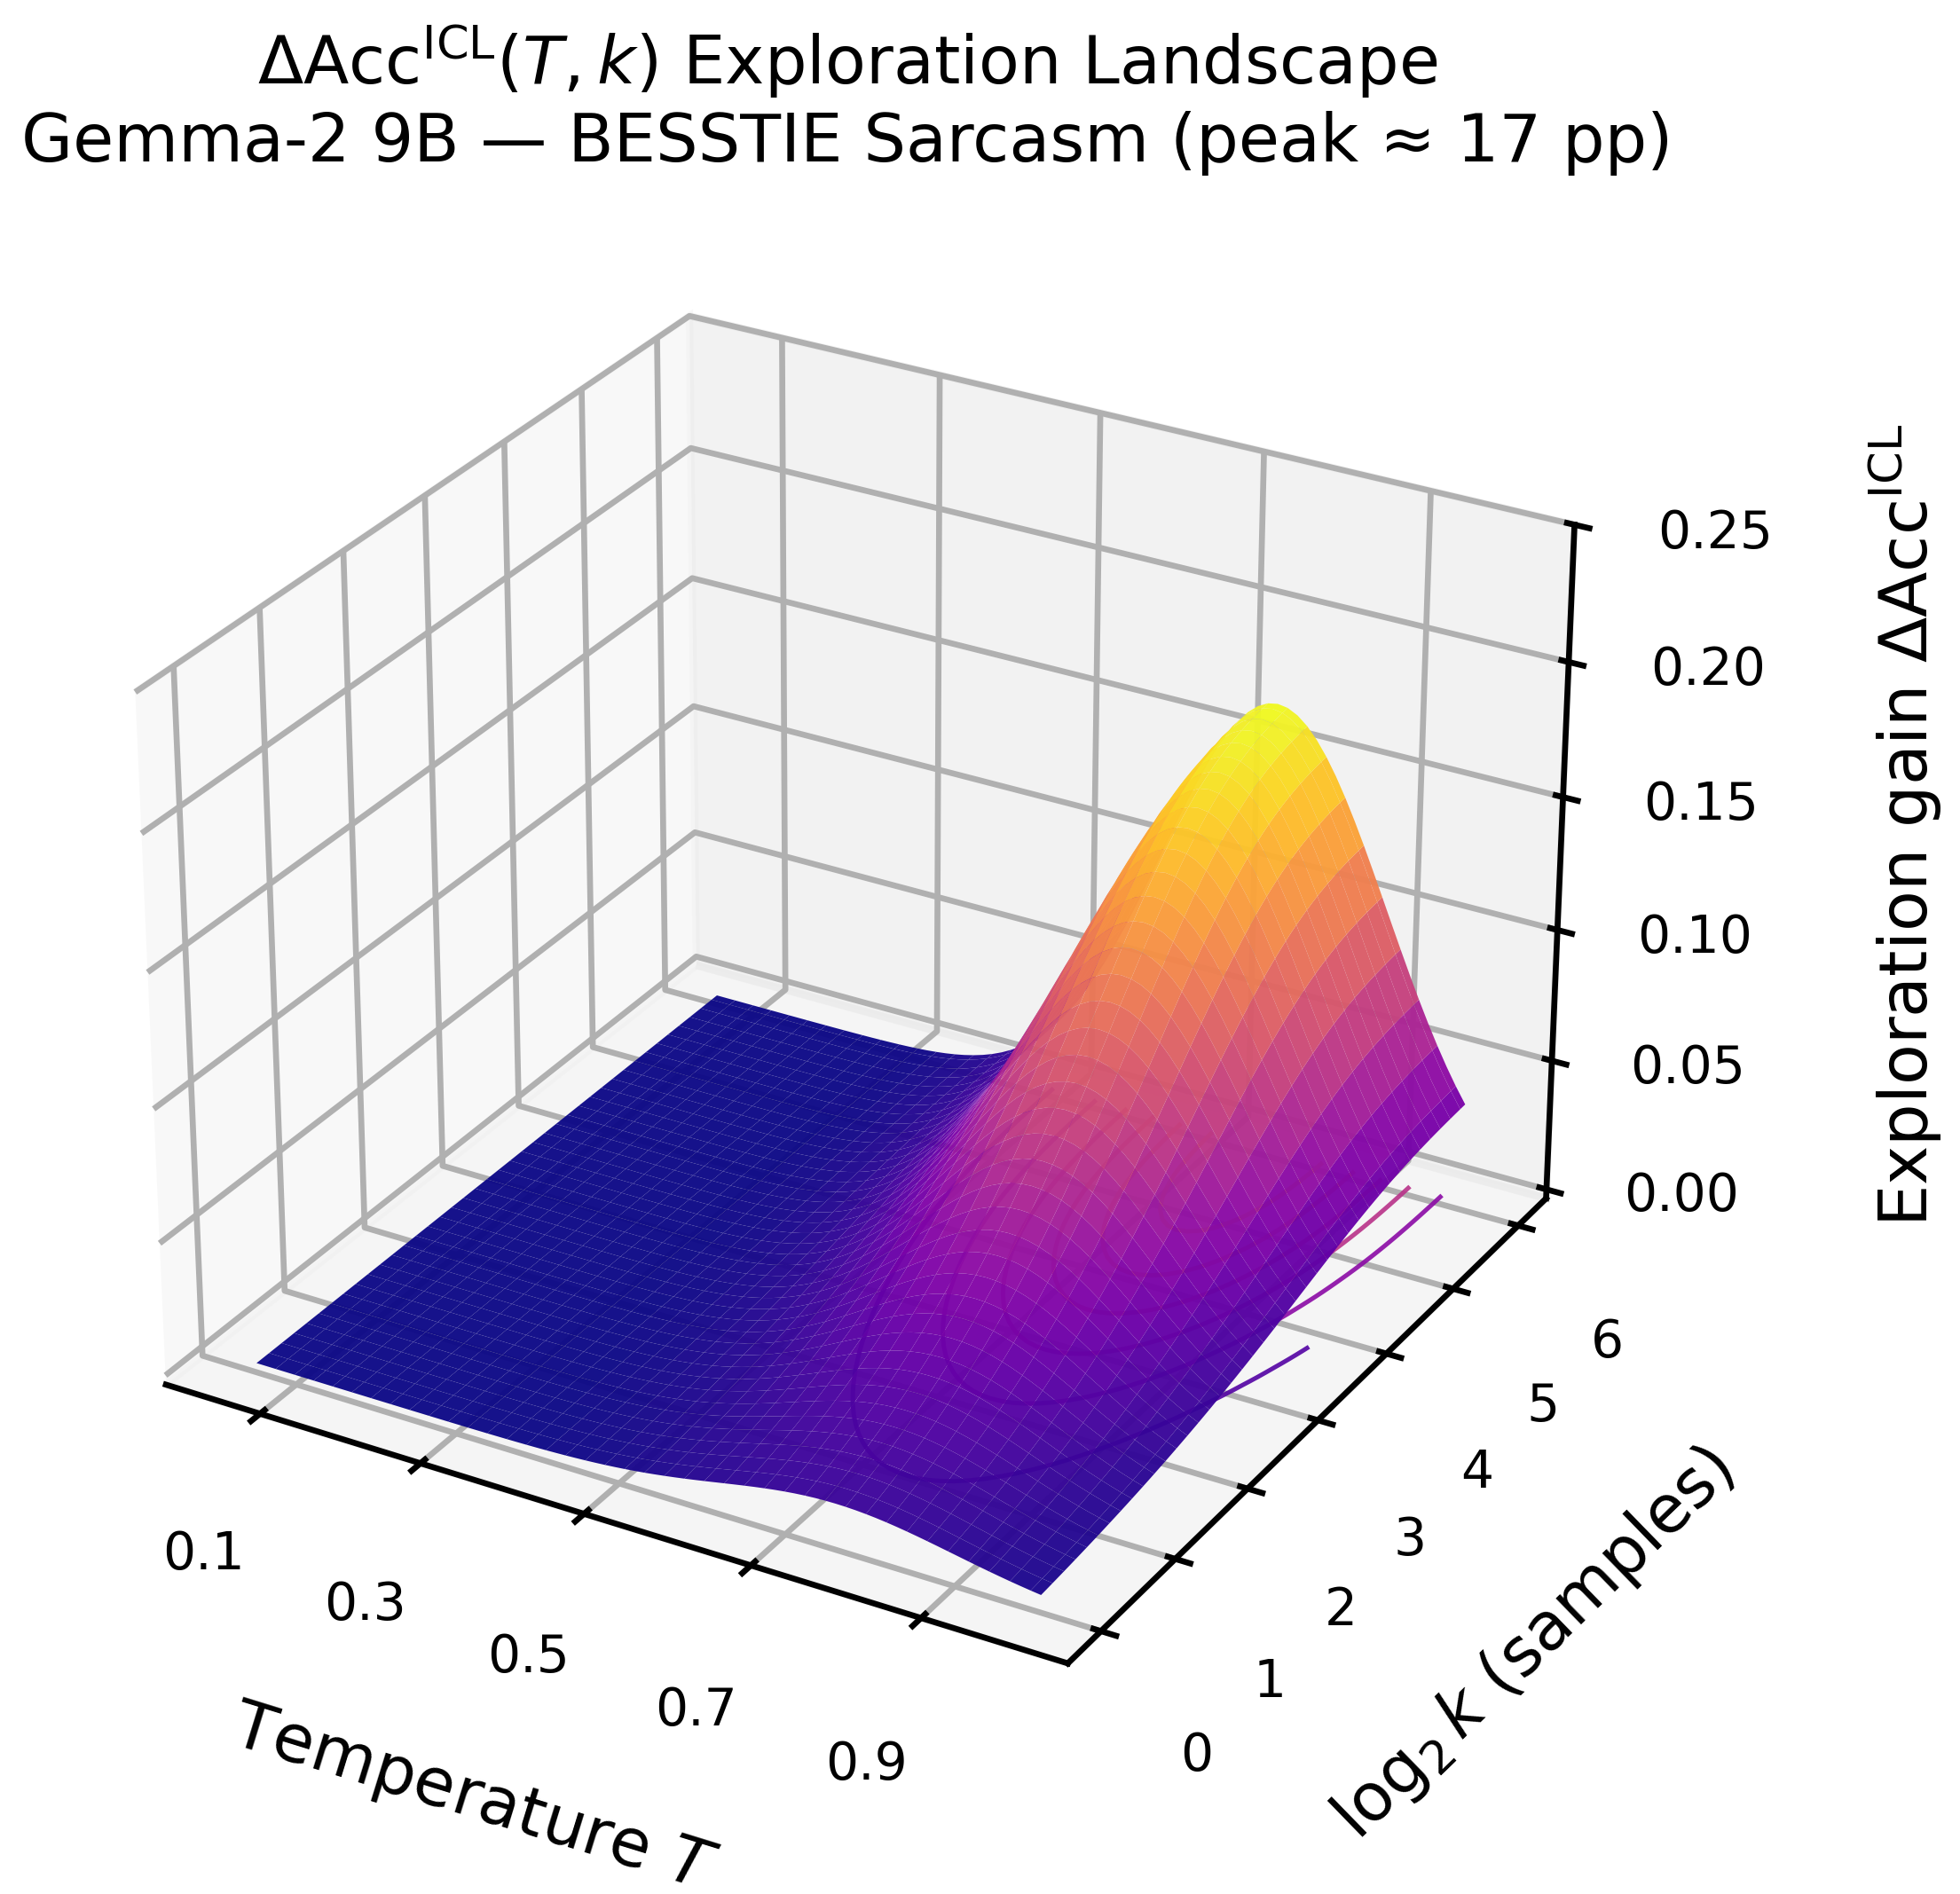
\includegraphics[width=\linewidth]{ICL/icl_exploration_landscape_Gemma_2_9B_sarcasm_parametric.png}
\end{minipage}
\caption{\textbf{Exploration--ICL landscapes for \textit{Gemma-2 9B}.}
\textbf{Left: Sentiment} shows a substantial ridge with peak gain $\mathbf{\approx 14}$\,pp, spanning $T \in [0.65,0.8]$ and $k \in [8,32]$, and quickly flattening for very low $k$ and overly hot temperatures.
\textbf{Right: Sarcasm} is even more exploration-sensitive, achieving a peak of $\mathbf{\approx 17}$\,pp and maintaining high gains over a wide band $T \in [0.65,0.85]$ and $k \in [8,48]$, where the surface height stays above roughly $0.10$ (i.e., $10$\,pp).
The color scale is again fixed to $[0,0.25]$, so the \emph{taller, warmer} ridge for sarcasm versus sentiment visually encodes a true difference in exploration headroom for the same backbone.}
\label{fig:icl_landscape_gemma2_9b}
\end{figure*}

% ===================== Gemma-2 27B =====================
\begin{figure*}[ht!]
\centering
\begin{minipage}{0.49\textwidth}
  \centering
  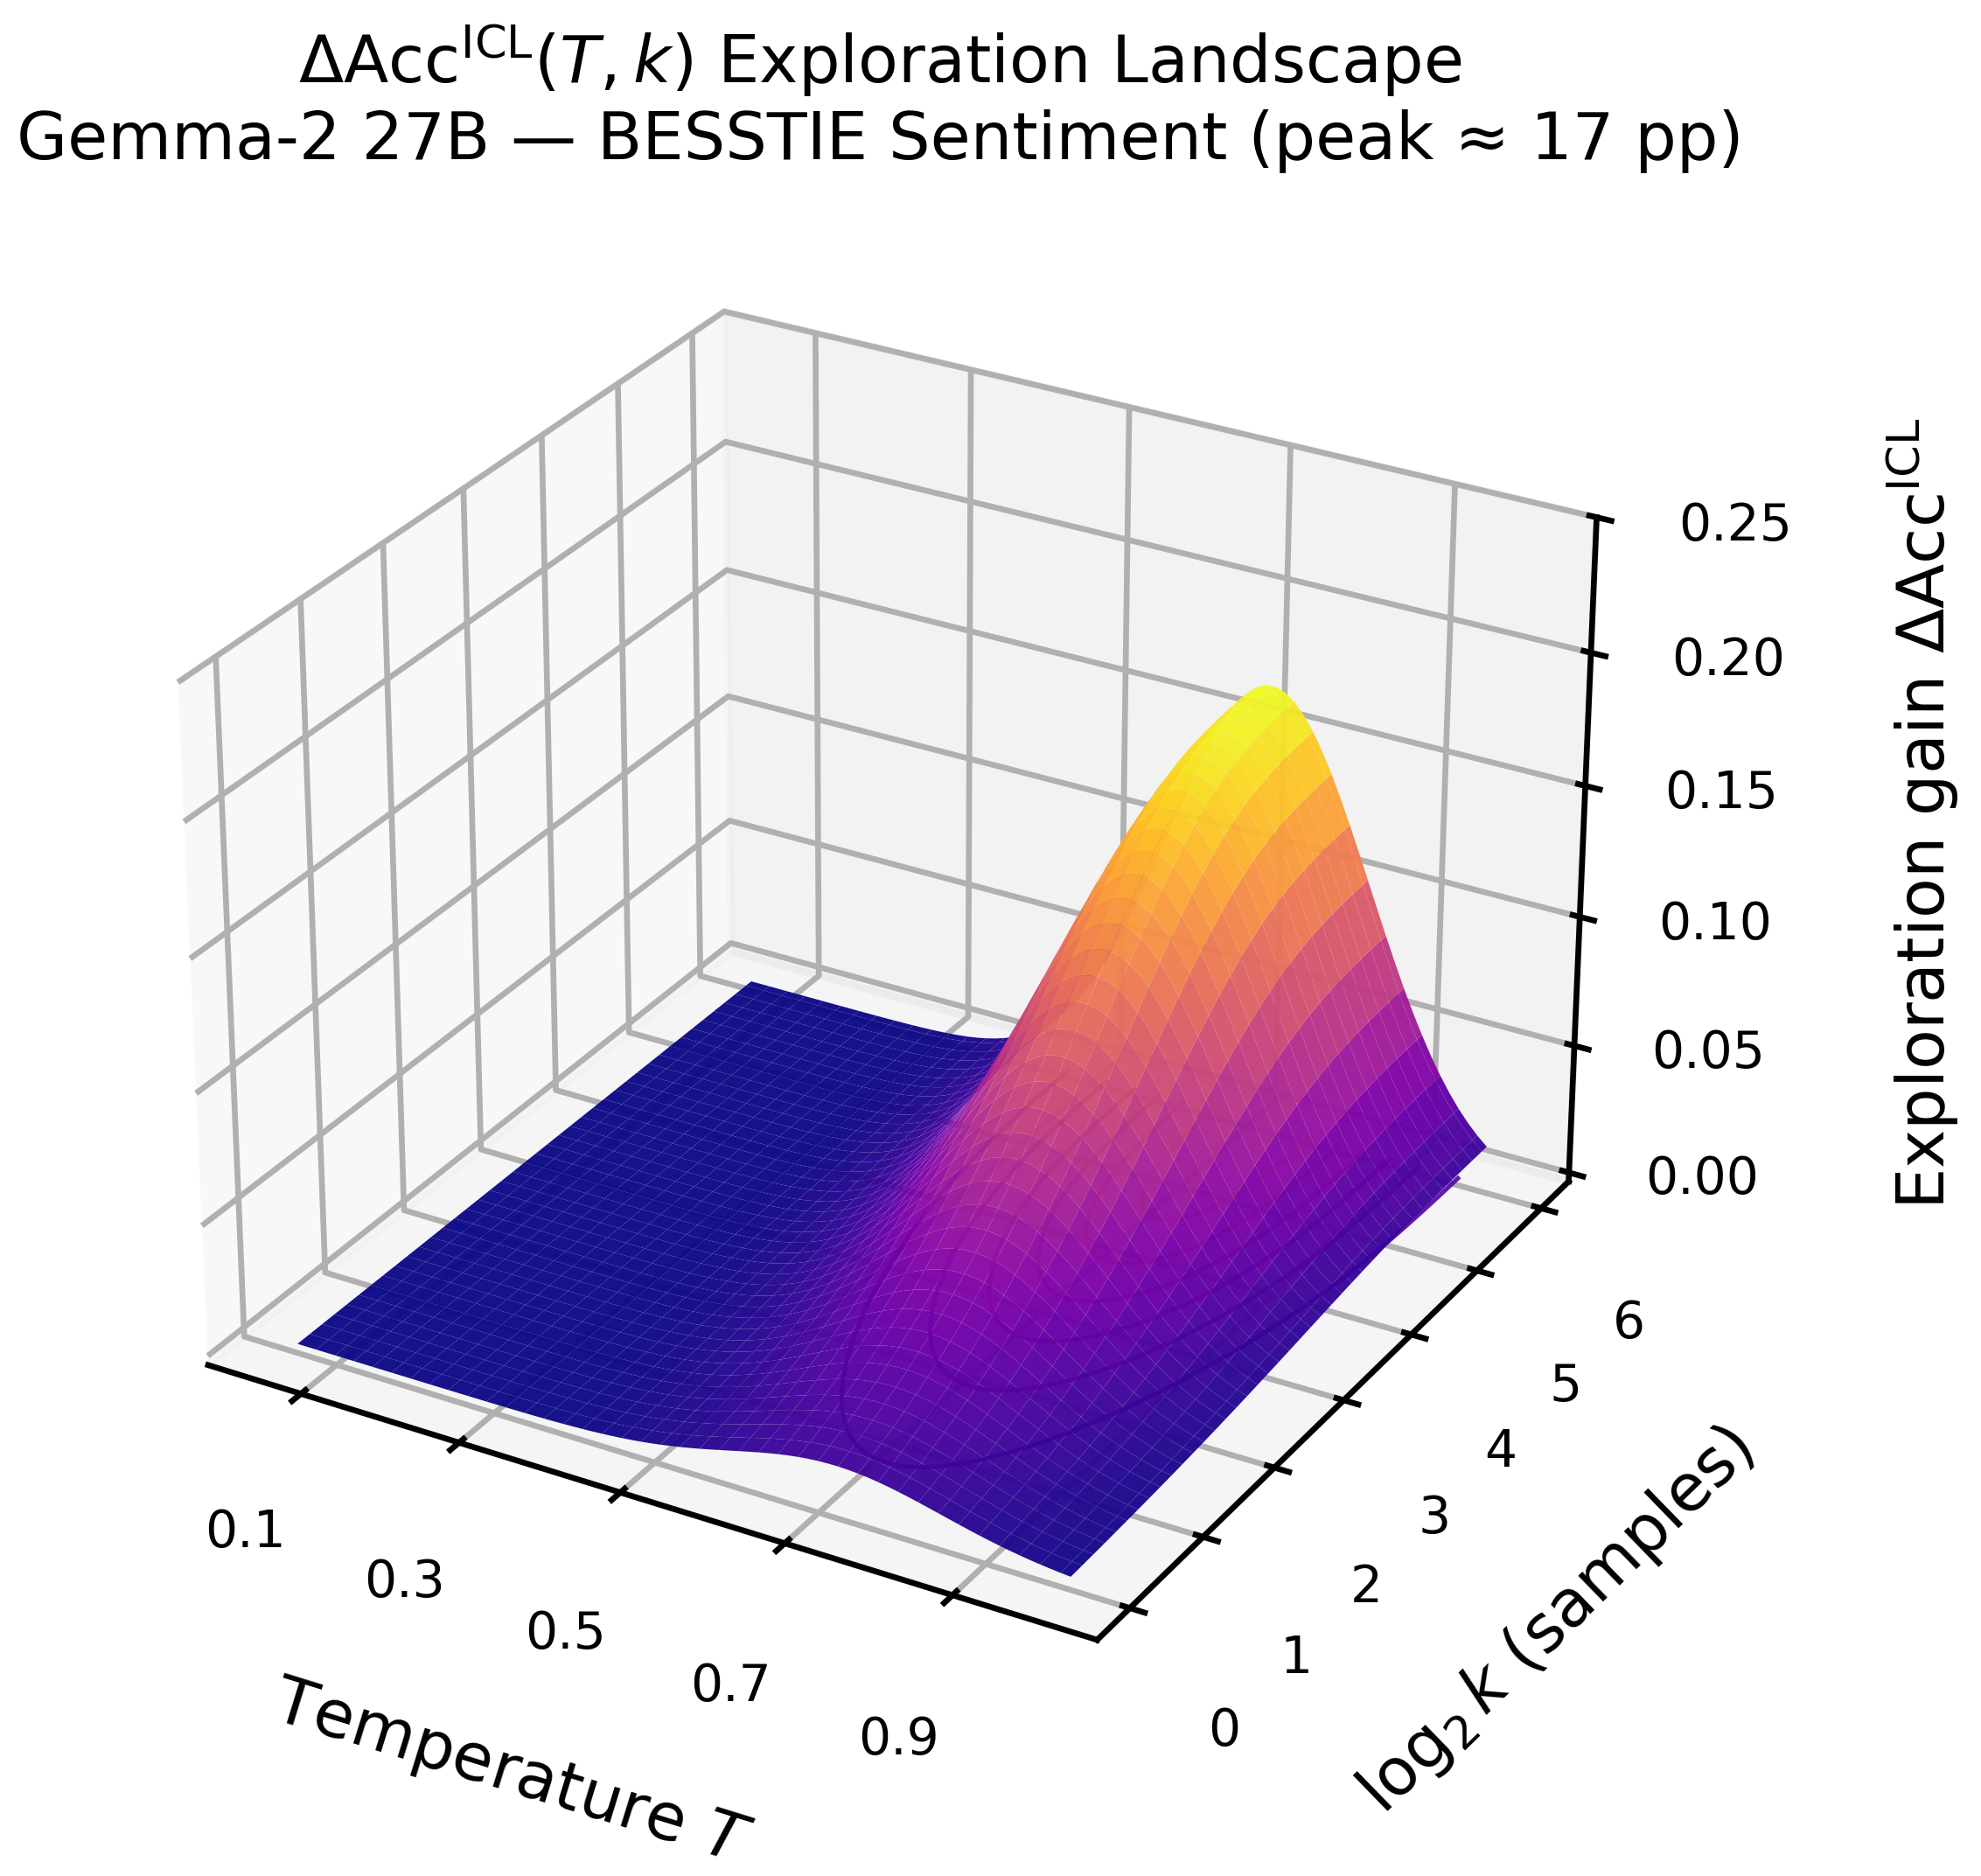
\includegraphics[width=\linewidth]{ICL/icl_exploration_landscape_Gemma_2_27B_sentiment_parametric.png}
\end{minipage}%
\hfill
\begin{minipage}{0.49\textwidth}
  \centering
  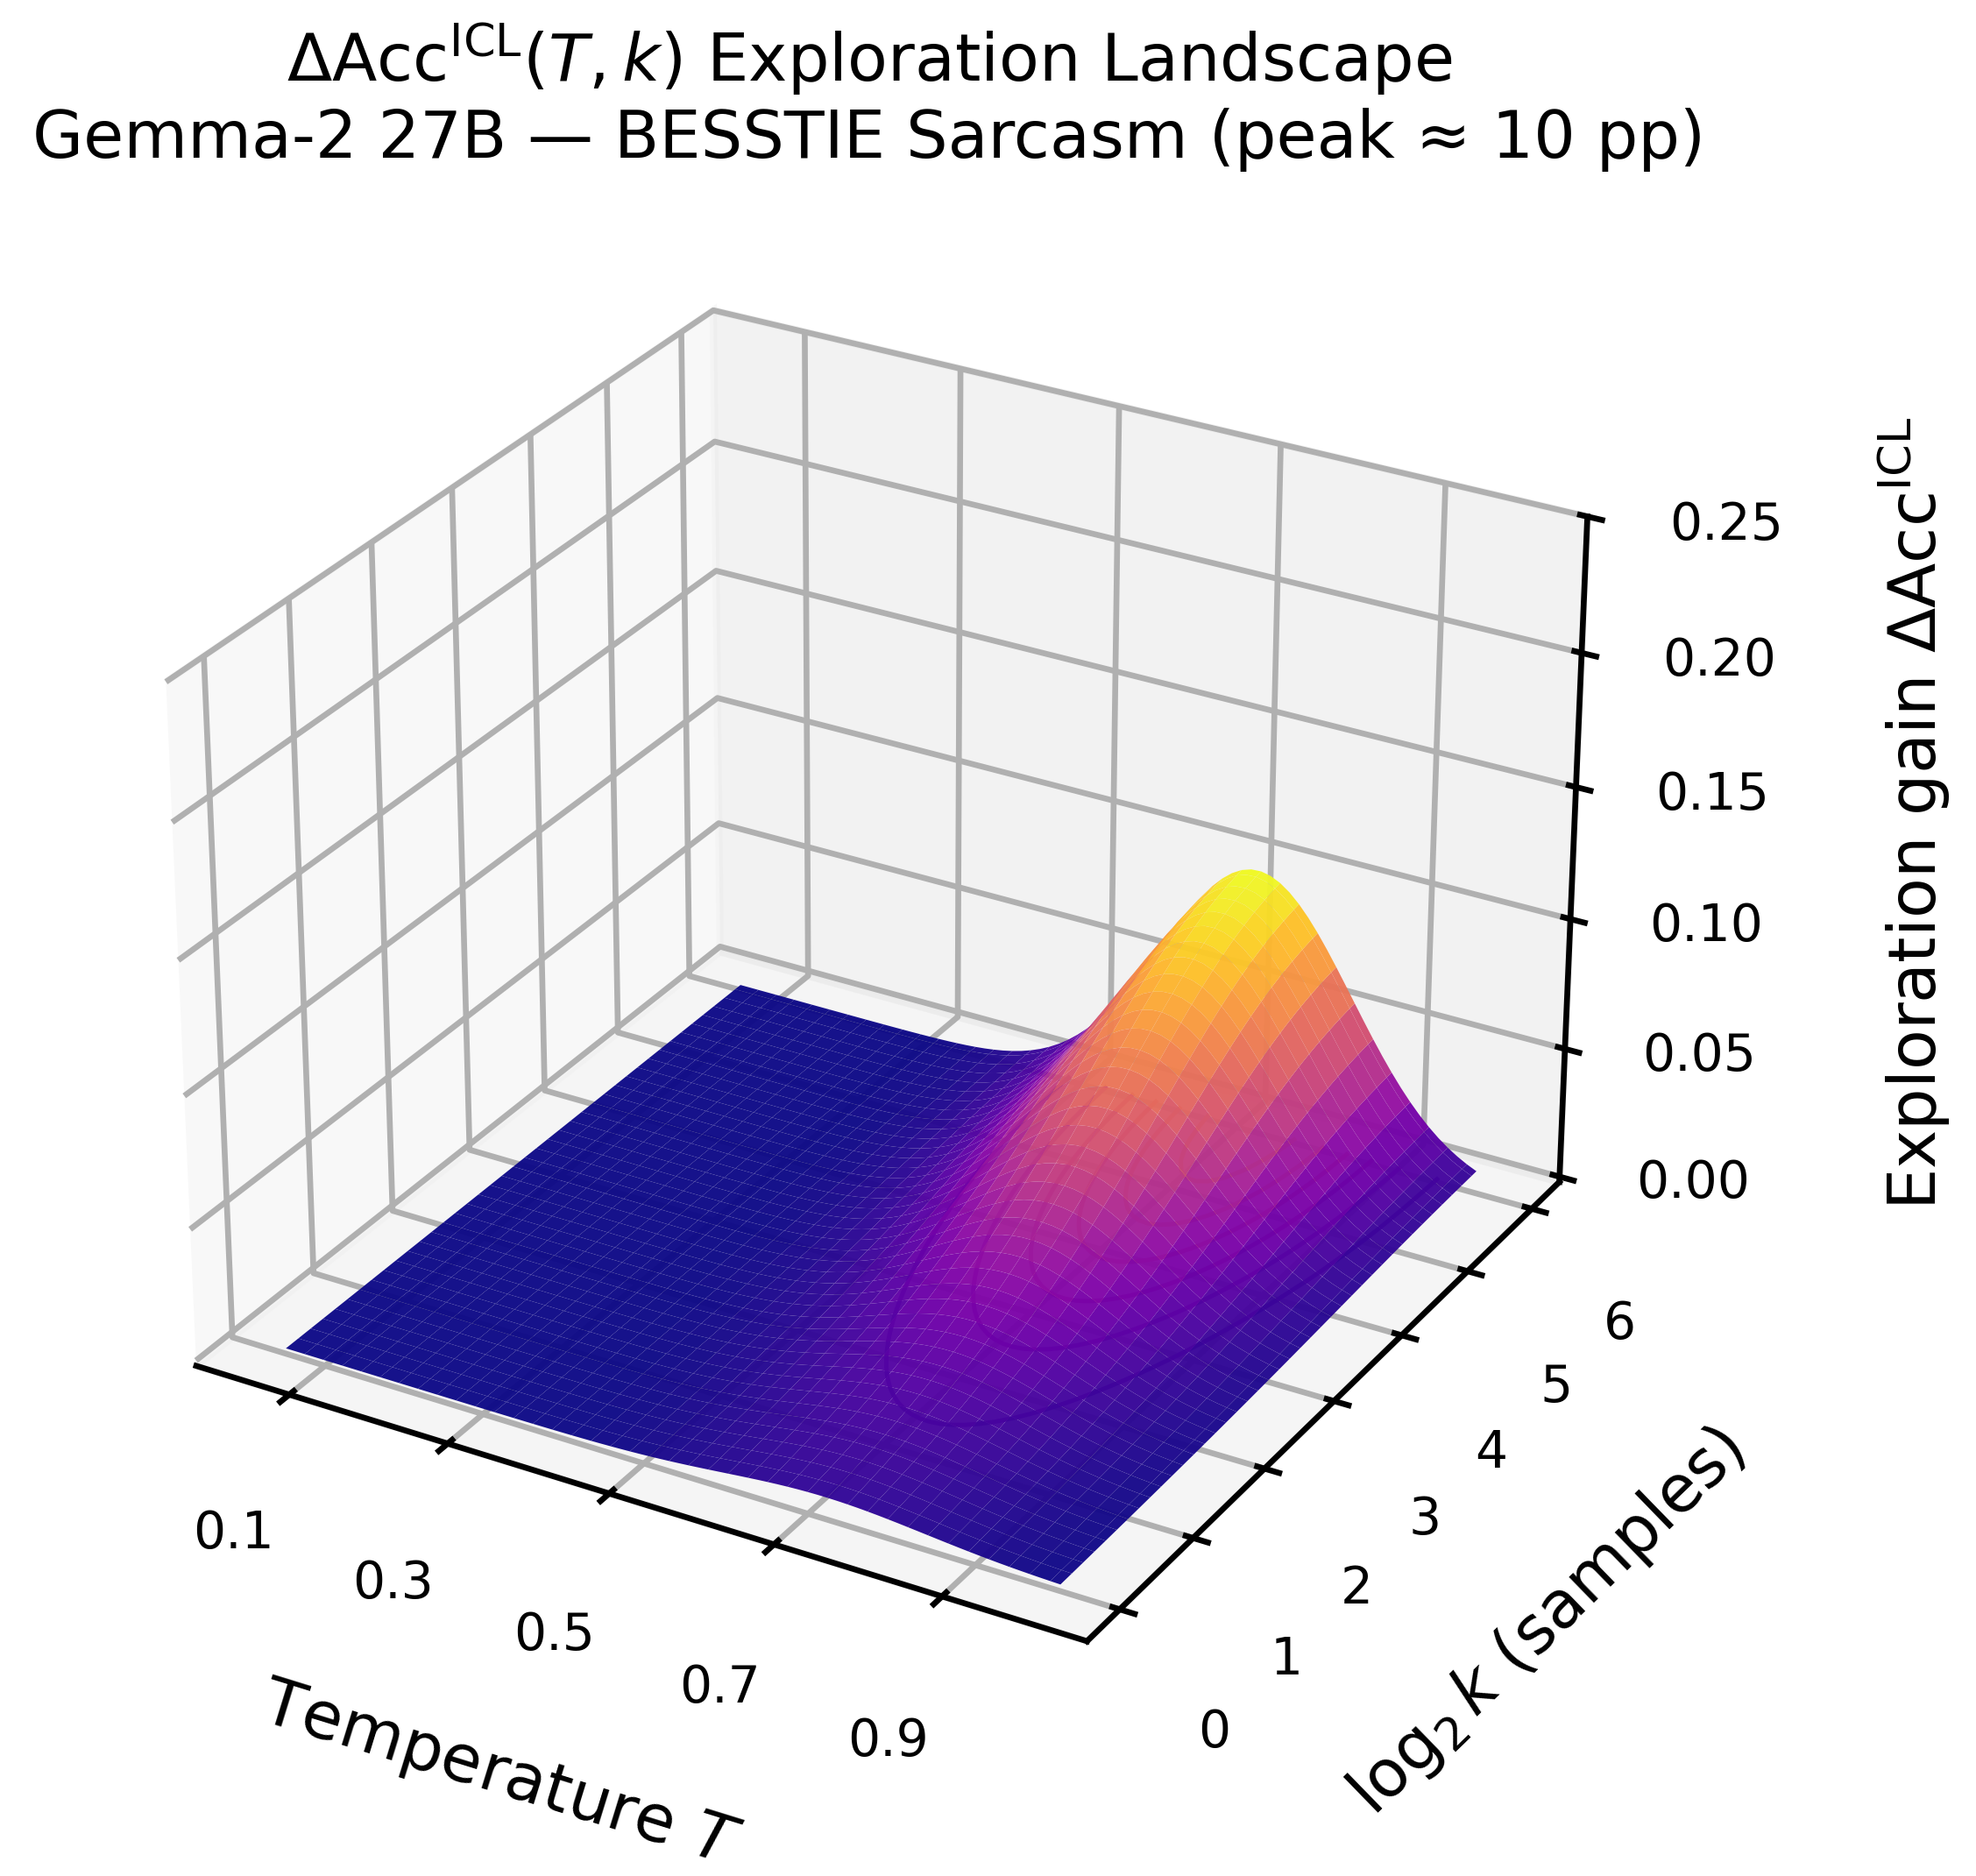
\includegraphics[width=\linewidth]{ICL/icl_exploration_landscape_Gemma_2_27B_sarcasm_parametric.png}
\end{minipage}
\caption{\textbf{Exploration--ICL landscapes for \textit{Gemma-2 27B}.}
\textbf{Left: Sentiment} exhibits one of the \emph{strongest} ridges in our study, with peak gain $\mathbf{\approx 17}$\,pp and a high plateau for $T \in [0.65,0.8]$ and $k \in [8,48]$, where $\Delta \mathrm{Acc}^{\mathrm{ICL}}$ remains in the $[0.10,0.20]$ (10--20\,pp) band.
\textbf{Right: Sarcasm} (peak $\mathbf{\approx 10}$\,pp) has a noticeably shorter and narrower ridge, concentrated near $T \approx 0.7$ and $k \in [8,24]$, suggesting that this larger Gemma variant is more exploration-hungry on sentiment than on sarcasm.
Because all panels share a common numeric range for $T$, $k$, and gain, the visual contrast between the left and right surfaces directly quantifies how task identity modulates the value of best-of-$k$ sampling.}
\label{fig:icl_landscape_gemma2_27b}
\end{figure*}

% ===================== Mistral-7B =====================
\begin{figure*}[ht!]
\centering
\begin{minipage}{0.49\textwidth}
  \centering
  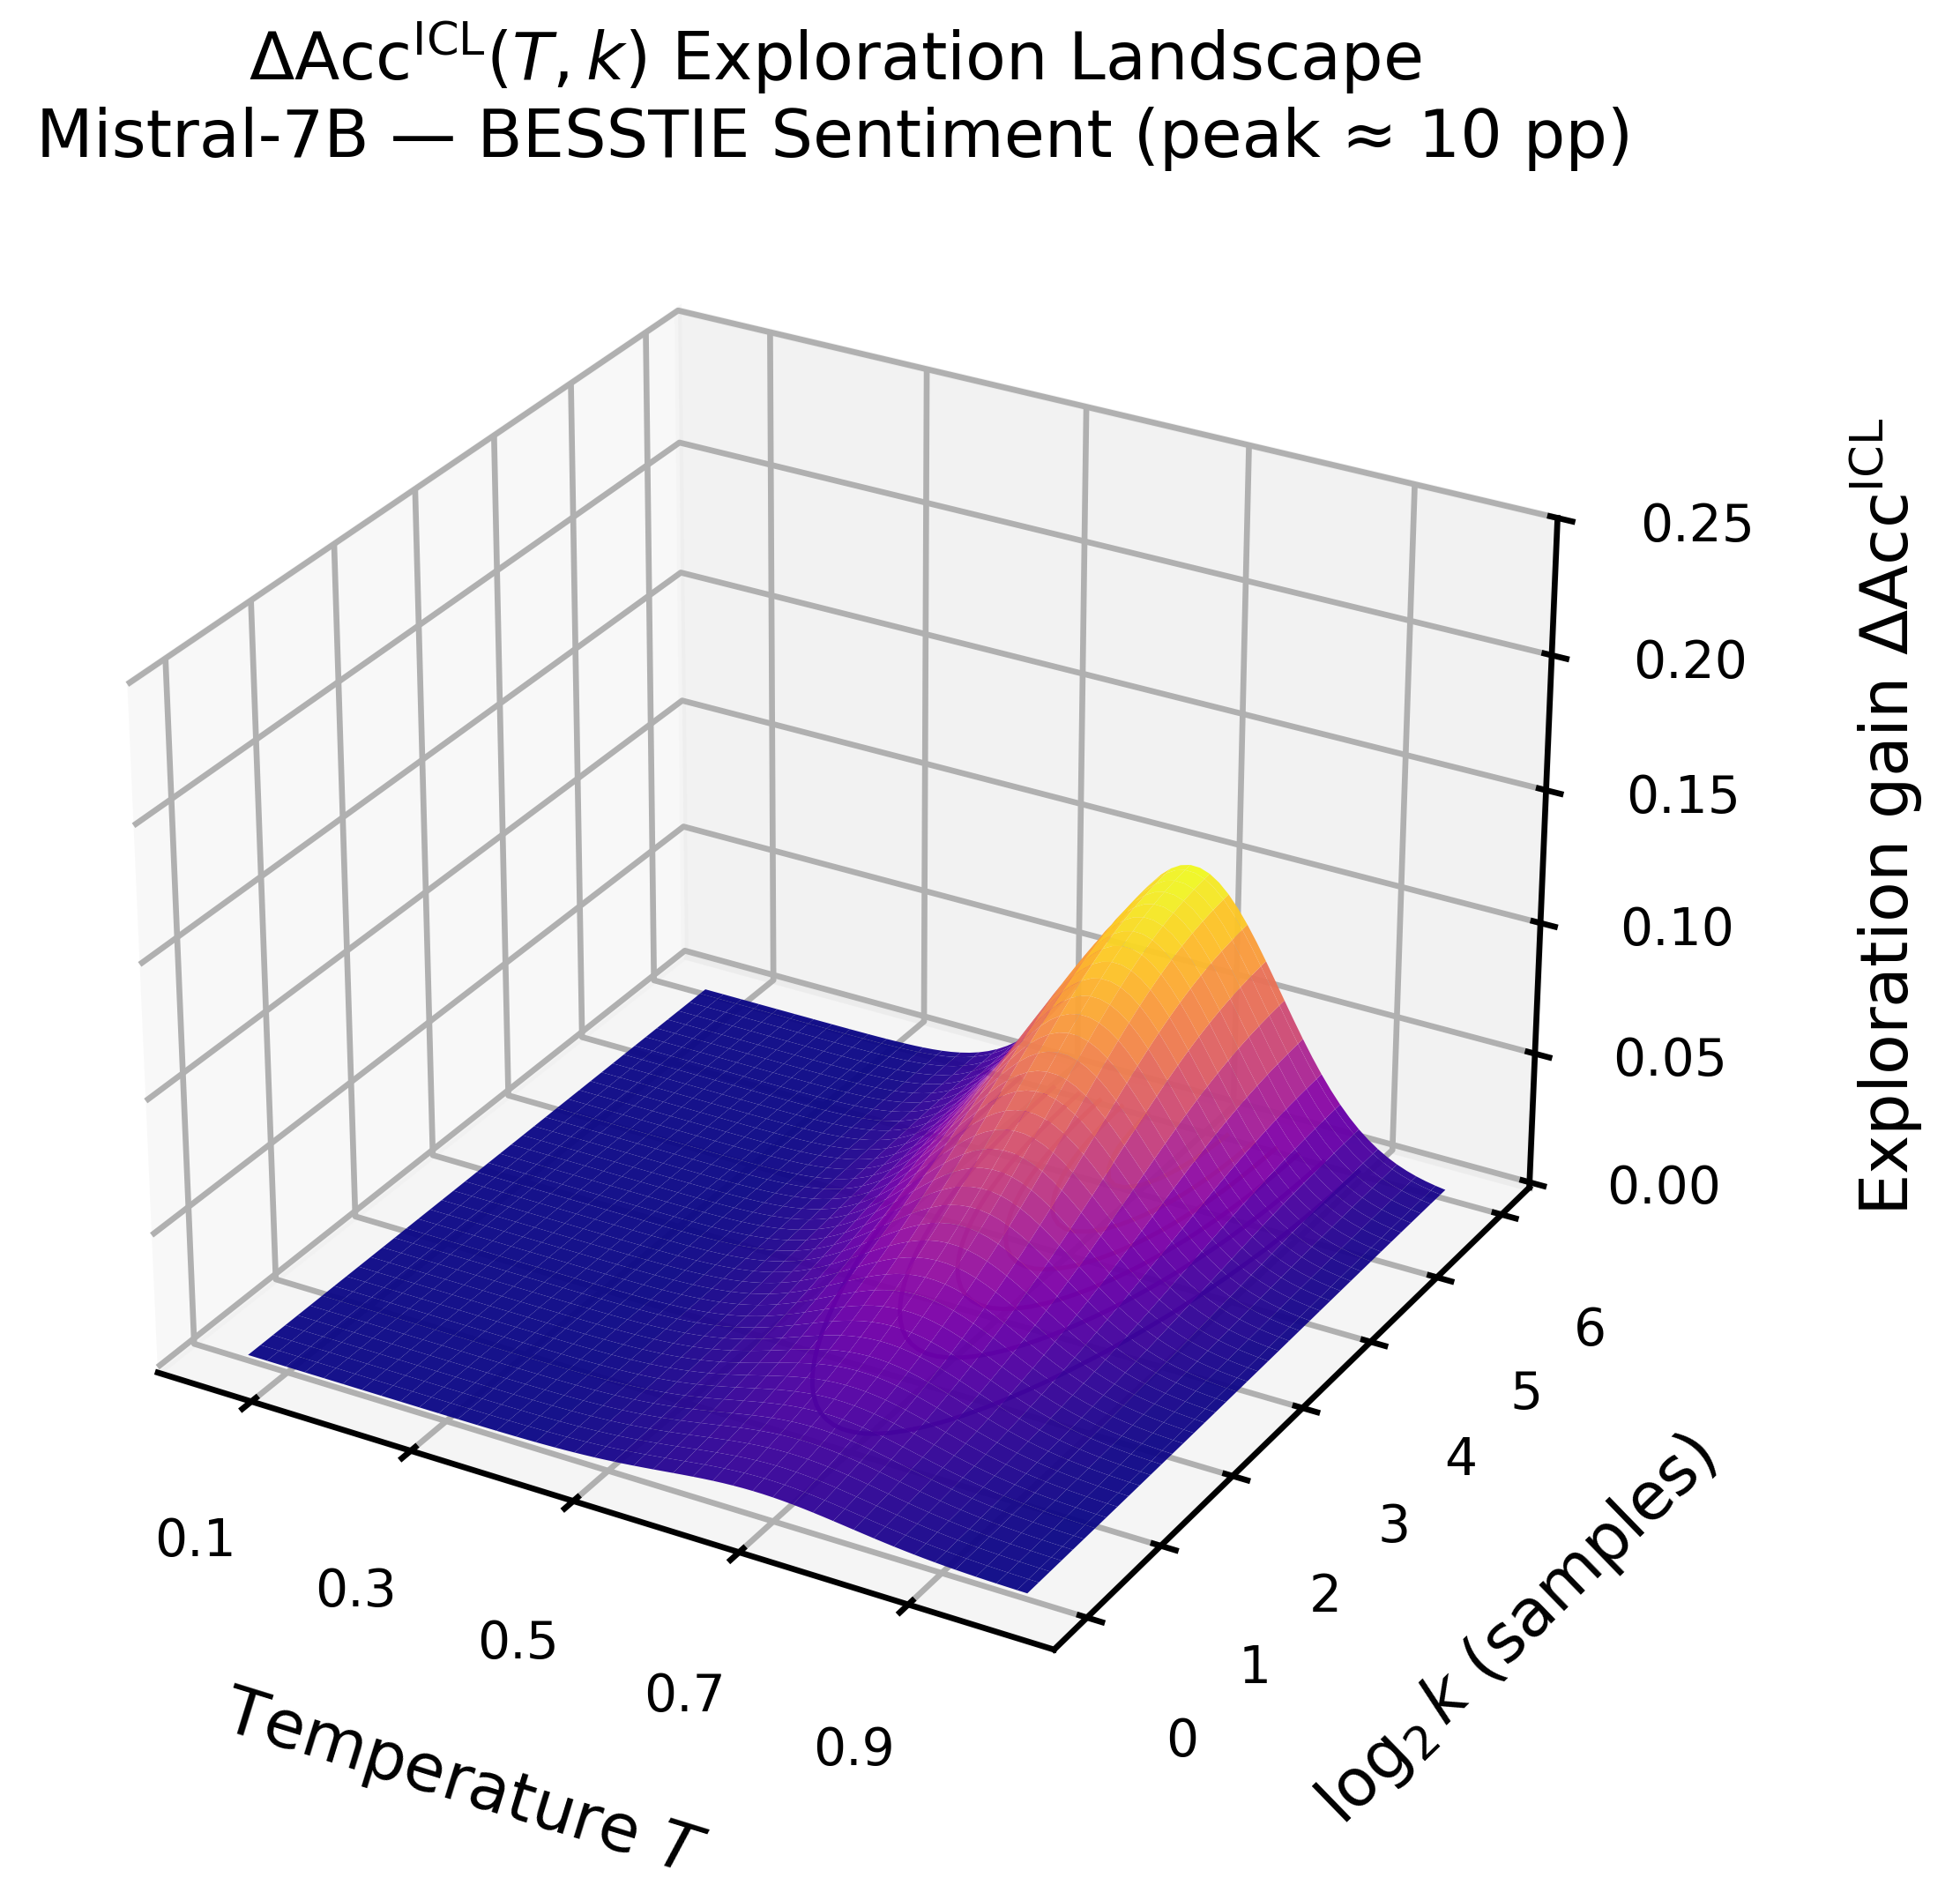
\includegraphics[width=\linewidth]{ICL/icl_exploration_landscape_Mistral_7B_sentiment_parametric.png}
\end{minipage}%
\hfill
\begin{minipage}{0.49\textwidth}
  \centering
  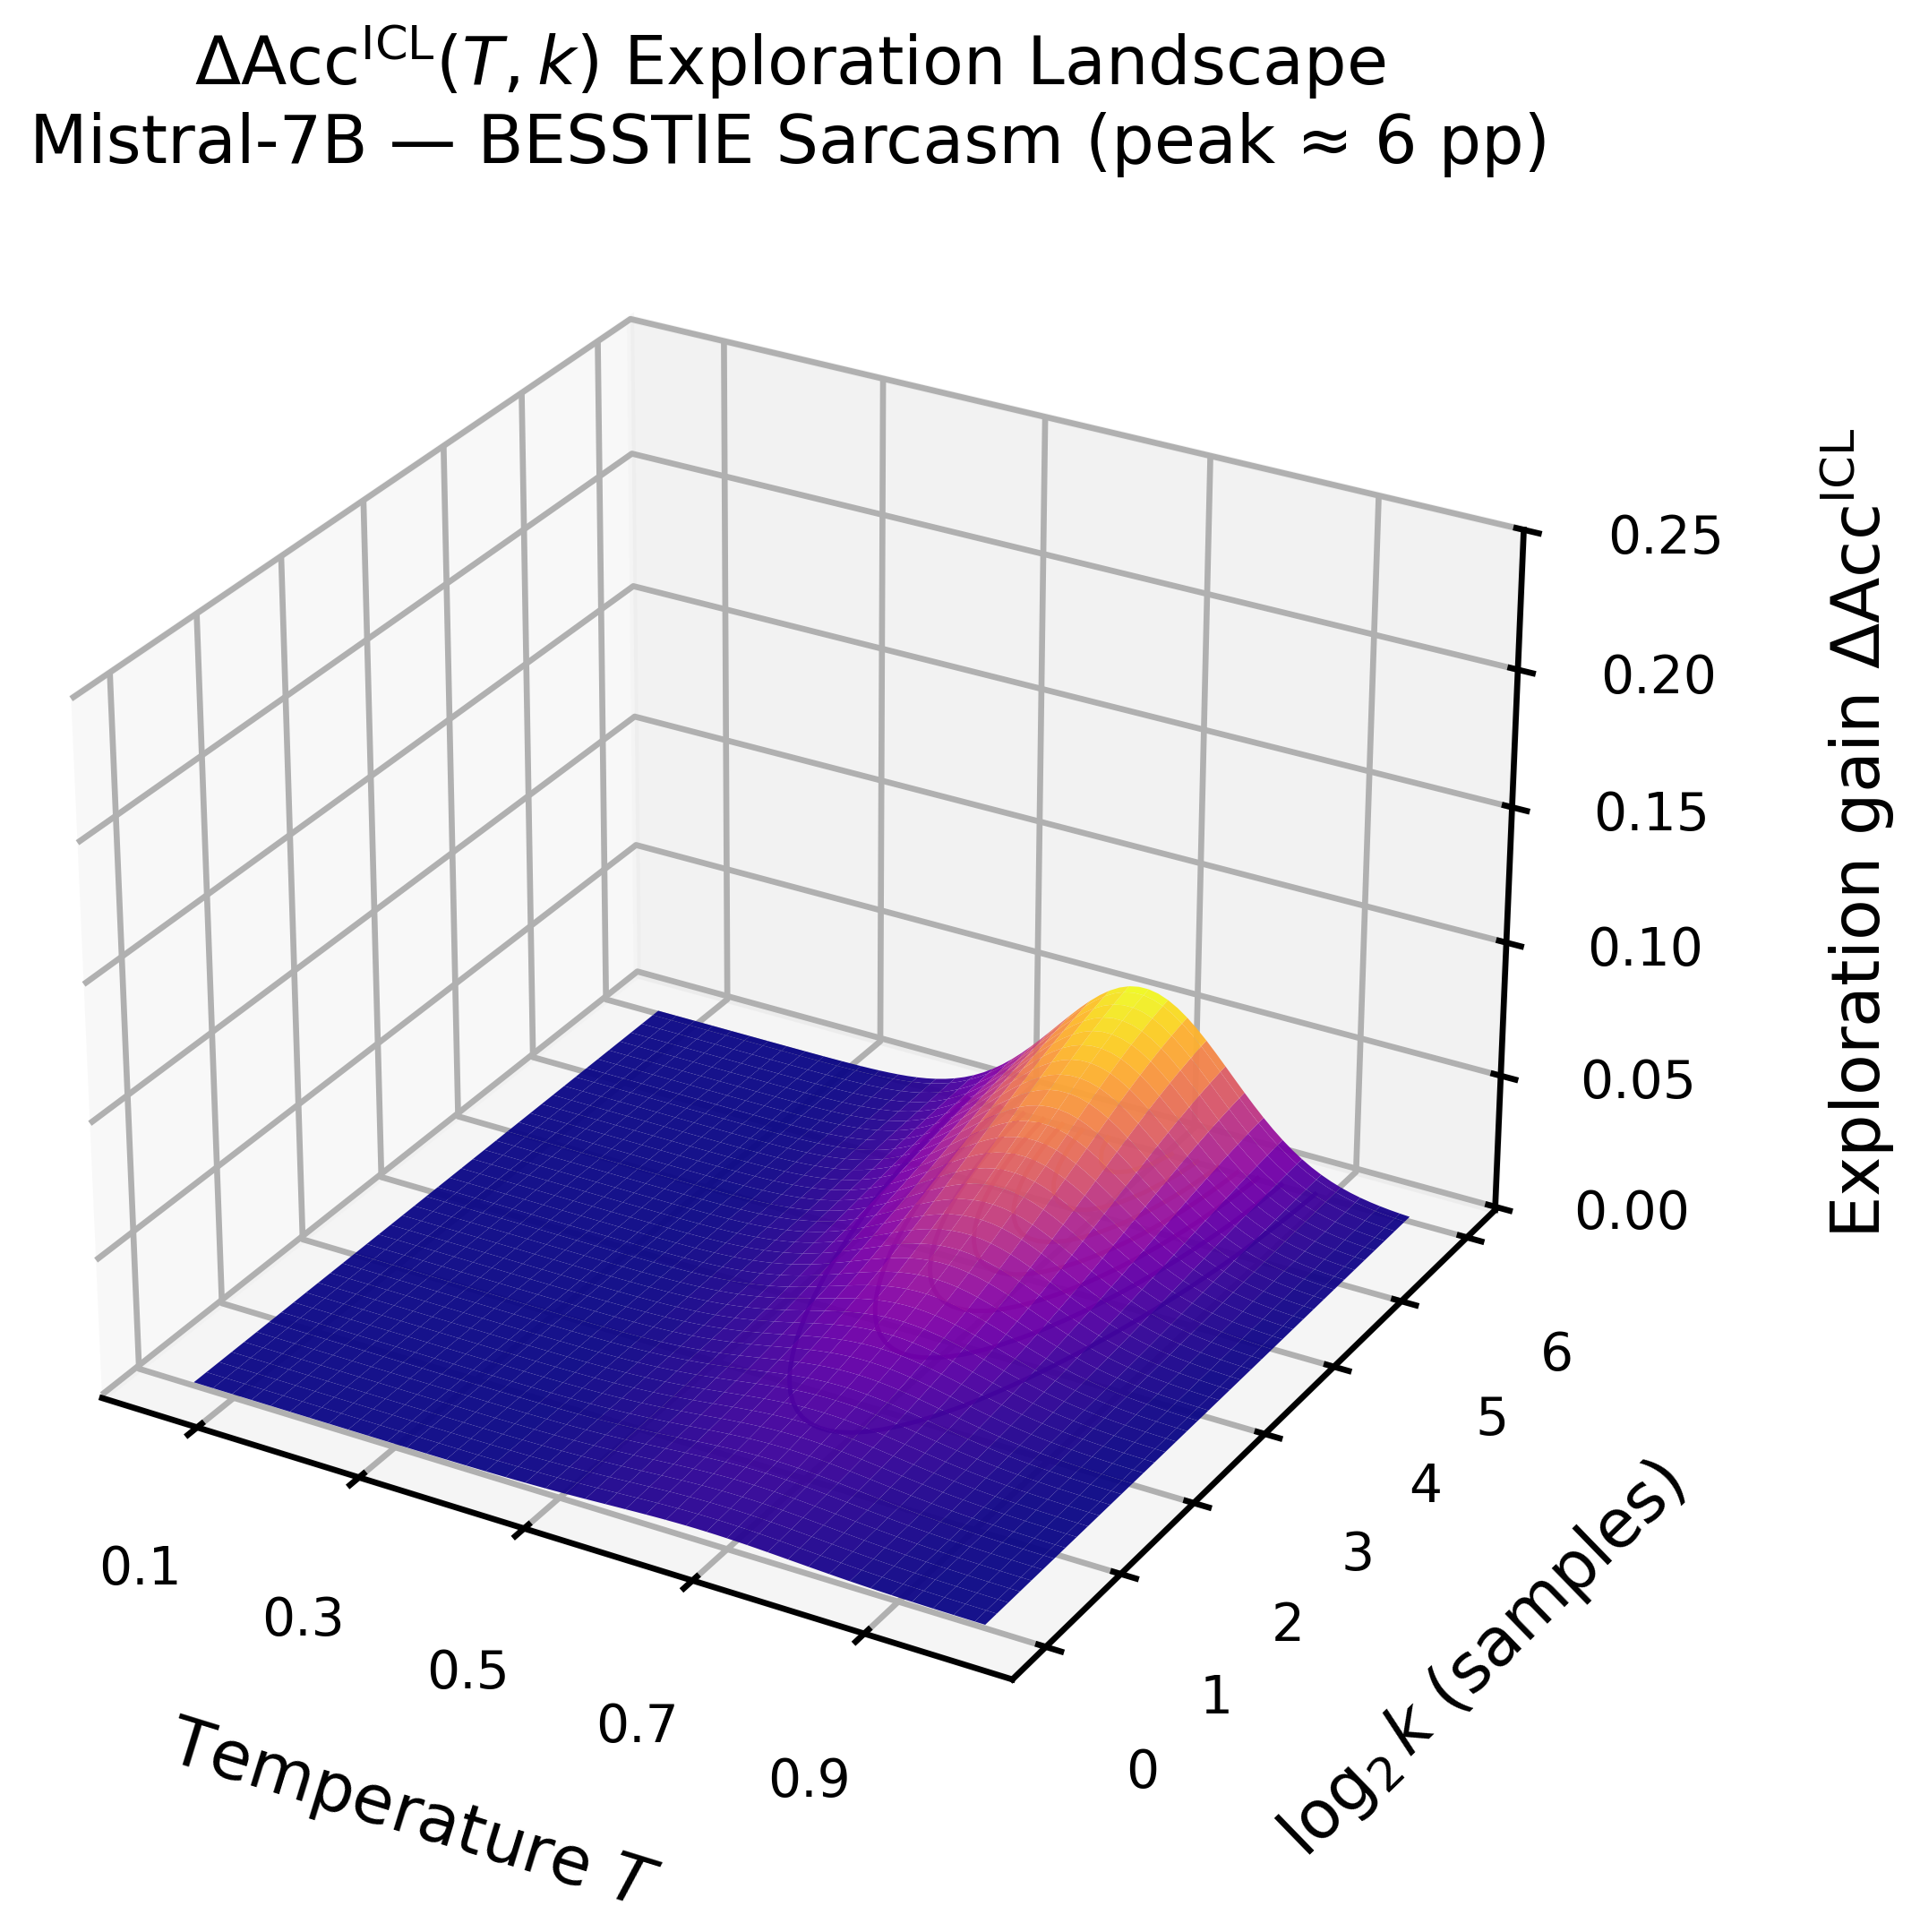
\includegraphics[width=\linewidth]{ICL/icl_exploration_landscape_Mistral_7B_sarcasm_parametric.png}
\end{minipage}
\caption{\textbf{Exploration--ICL landscapes for \textit{Mistral-7B}.}
\textbf{Left: Sentiment} (peak gain $\mathbf{\approx 10}$\,pp) has a clean, single ridge around $T \approx 0.7$ and $k \in [8,24]$; below $k=4$ or above $k=32$ the surface rapidly collapses toward $0$.
\textbf{Right: Sarcasm} (peak $\mathbf{\approx 6}$\,pp) is noticeably flatter and lower, with only a mild bump in the same approximate $(T,k)$ region, showing that this backbone is less reliant on exploration to solve sarcastic prompts.
Within the global numeric ranges $T \in [0.05,1.0]$, $\log_2 k \in [0,6]$, and $\Delta \mathrm{Acc}^{\mathrm{ICL}} \in [0,0.25]$, Mistral-7B thus appears as a model where exploration is \emph{useful but not critical}, especially relative to Gemma-2.}
\label{fig:icl_landscape_mistral7b}
\end{figure*}

% ===================== Mixtral-8x7B =====================
\begin{figure*}[ht!]
\centering
\begin{minipage}{0.49\textwidth}
  \centering
  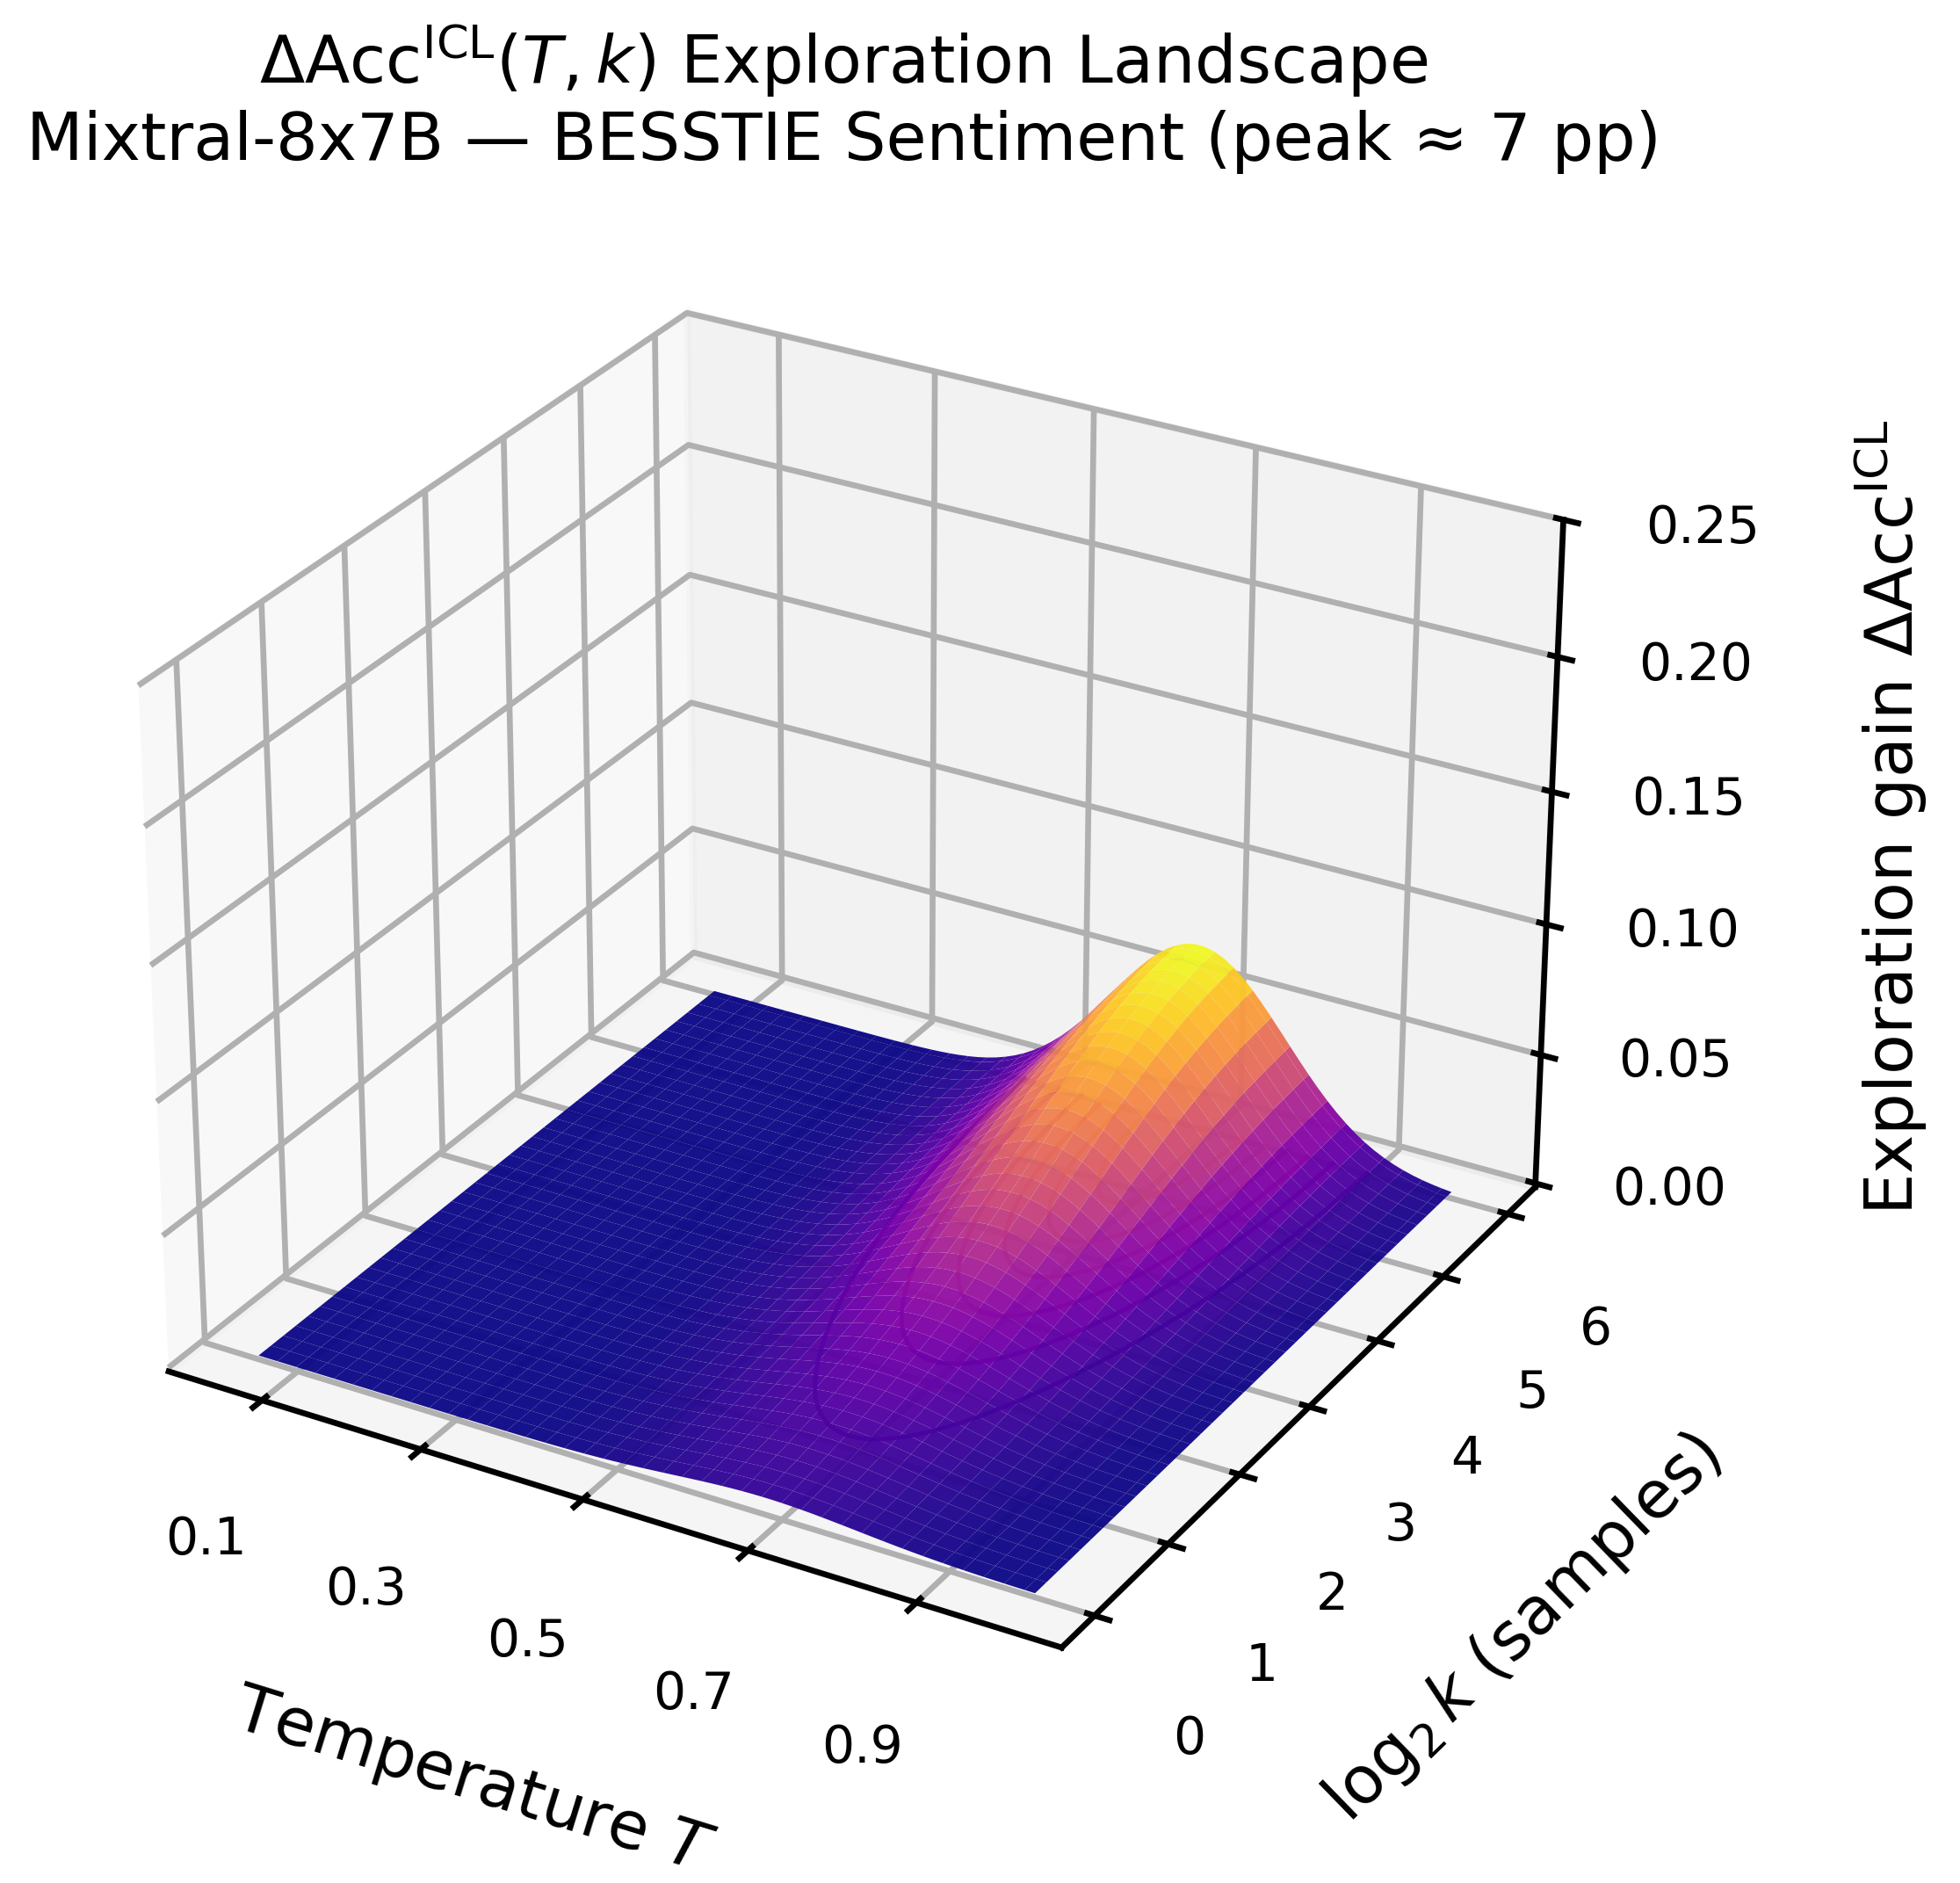
\includegraphics[width=\linewidth]{ICL/icl_exploration_landscape_Mixtral_8x7B_sentiment_parametric.png}
\end{minipage}%
\hfill
\begin{minipage}{0.49\textwidth}
  \centering
  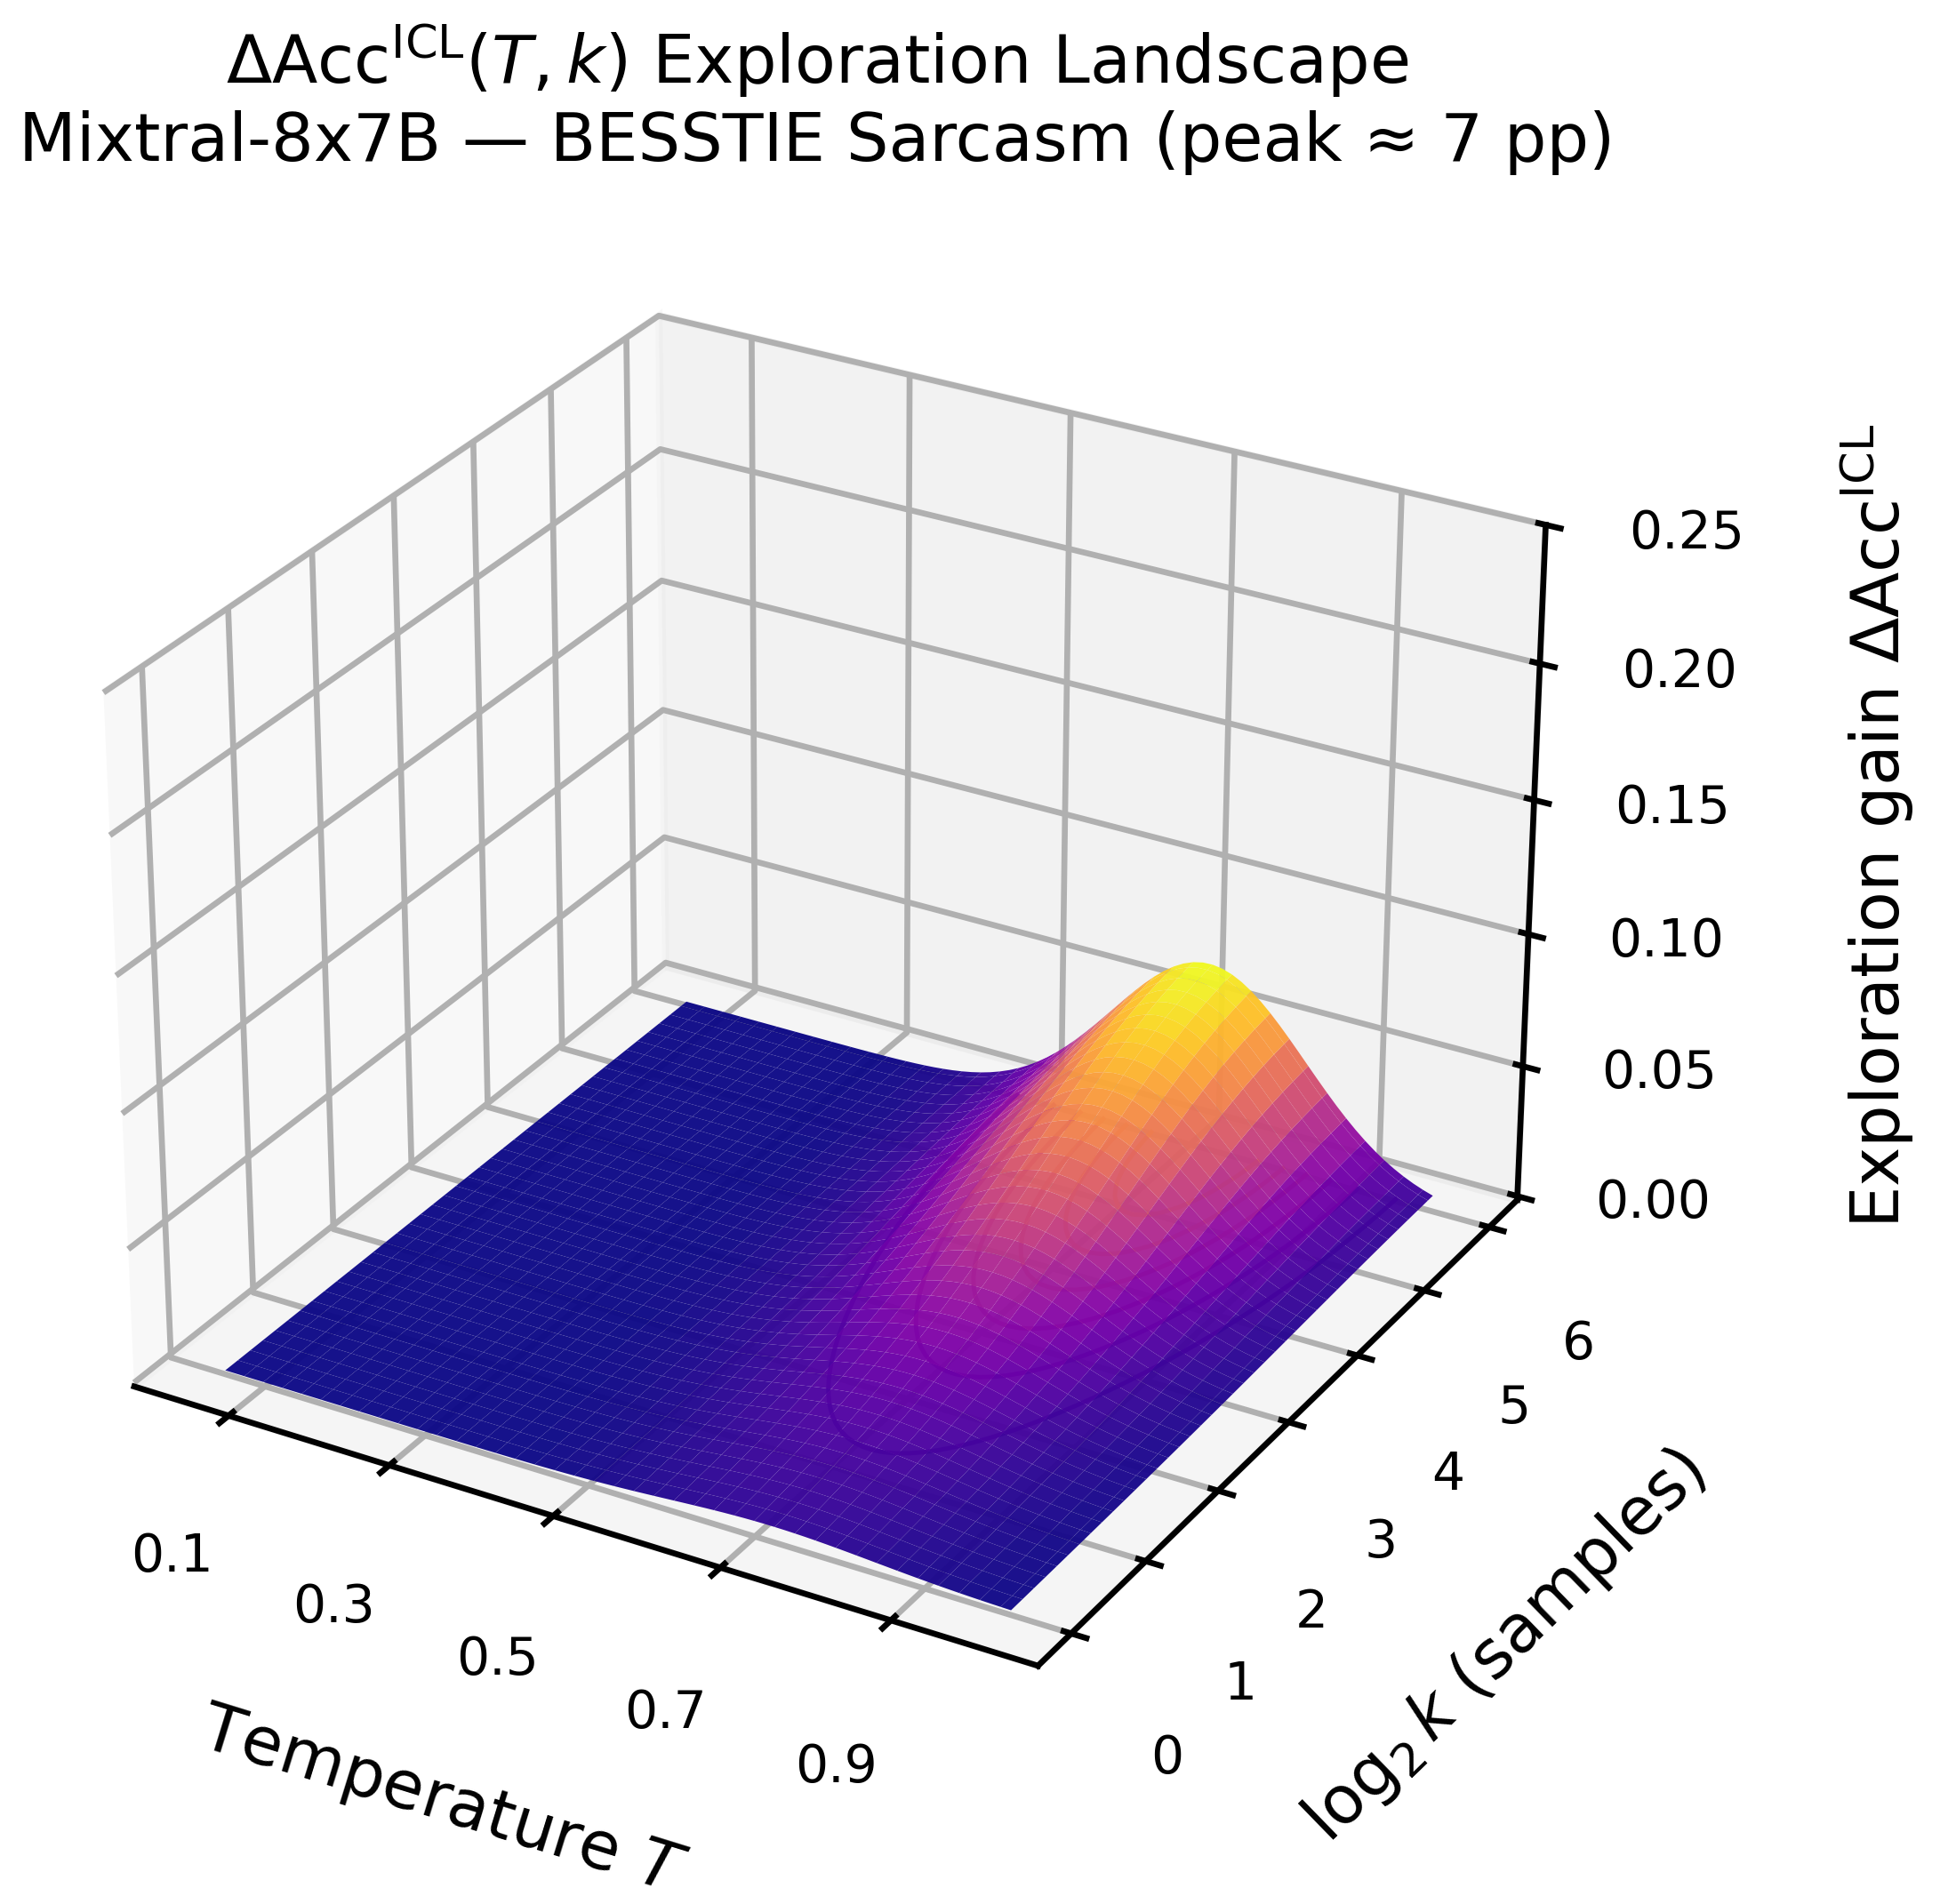
\includegraphics[width=\linewidth]{ICL/icl_exploration_landscape_Mixtral_8x7B_sarcasm_parametric.png}
\end{minipage}
\caption{\textbf{Exploration--ICL landscapes for \textit{Mixtral-8x7B}.}
\textbf{Left: Sentiment} and \textbf{Right: Sarcasm} both peak at roughly $\mathbf{\approx 7}$\,pp, with gently sloping ridges around $T \in [0.65,0.8]$ and $k \in [8,24]$.
The similarity of the two surfaces---both staying mostly within the $[0.03,0.12]$ gain band (3--12\,pp) across the high-exploration region---suggests that the MoE routing in Mixtral-8x7B introduces a fairly \emph{task-agnostic} response to best-of-$k$ sampling.
Overall, the numeric ranges confirm that this model sees consistent but moderate exploration benefits across both sentiment and sarcasm, with no extreme dependence on temperature or very large $k$.}
\label{fig:icl_landscape_mixtral_8x7b}
\end{figure*}

% ===================== Mixtral-8x22B =====================
\begin{figure*}[ht!]
\centering
\begin{minipage}{0.49\textwidth}
  \centering
  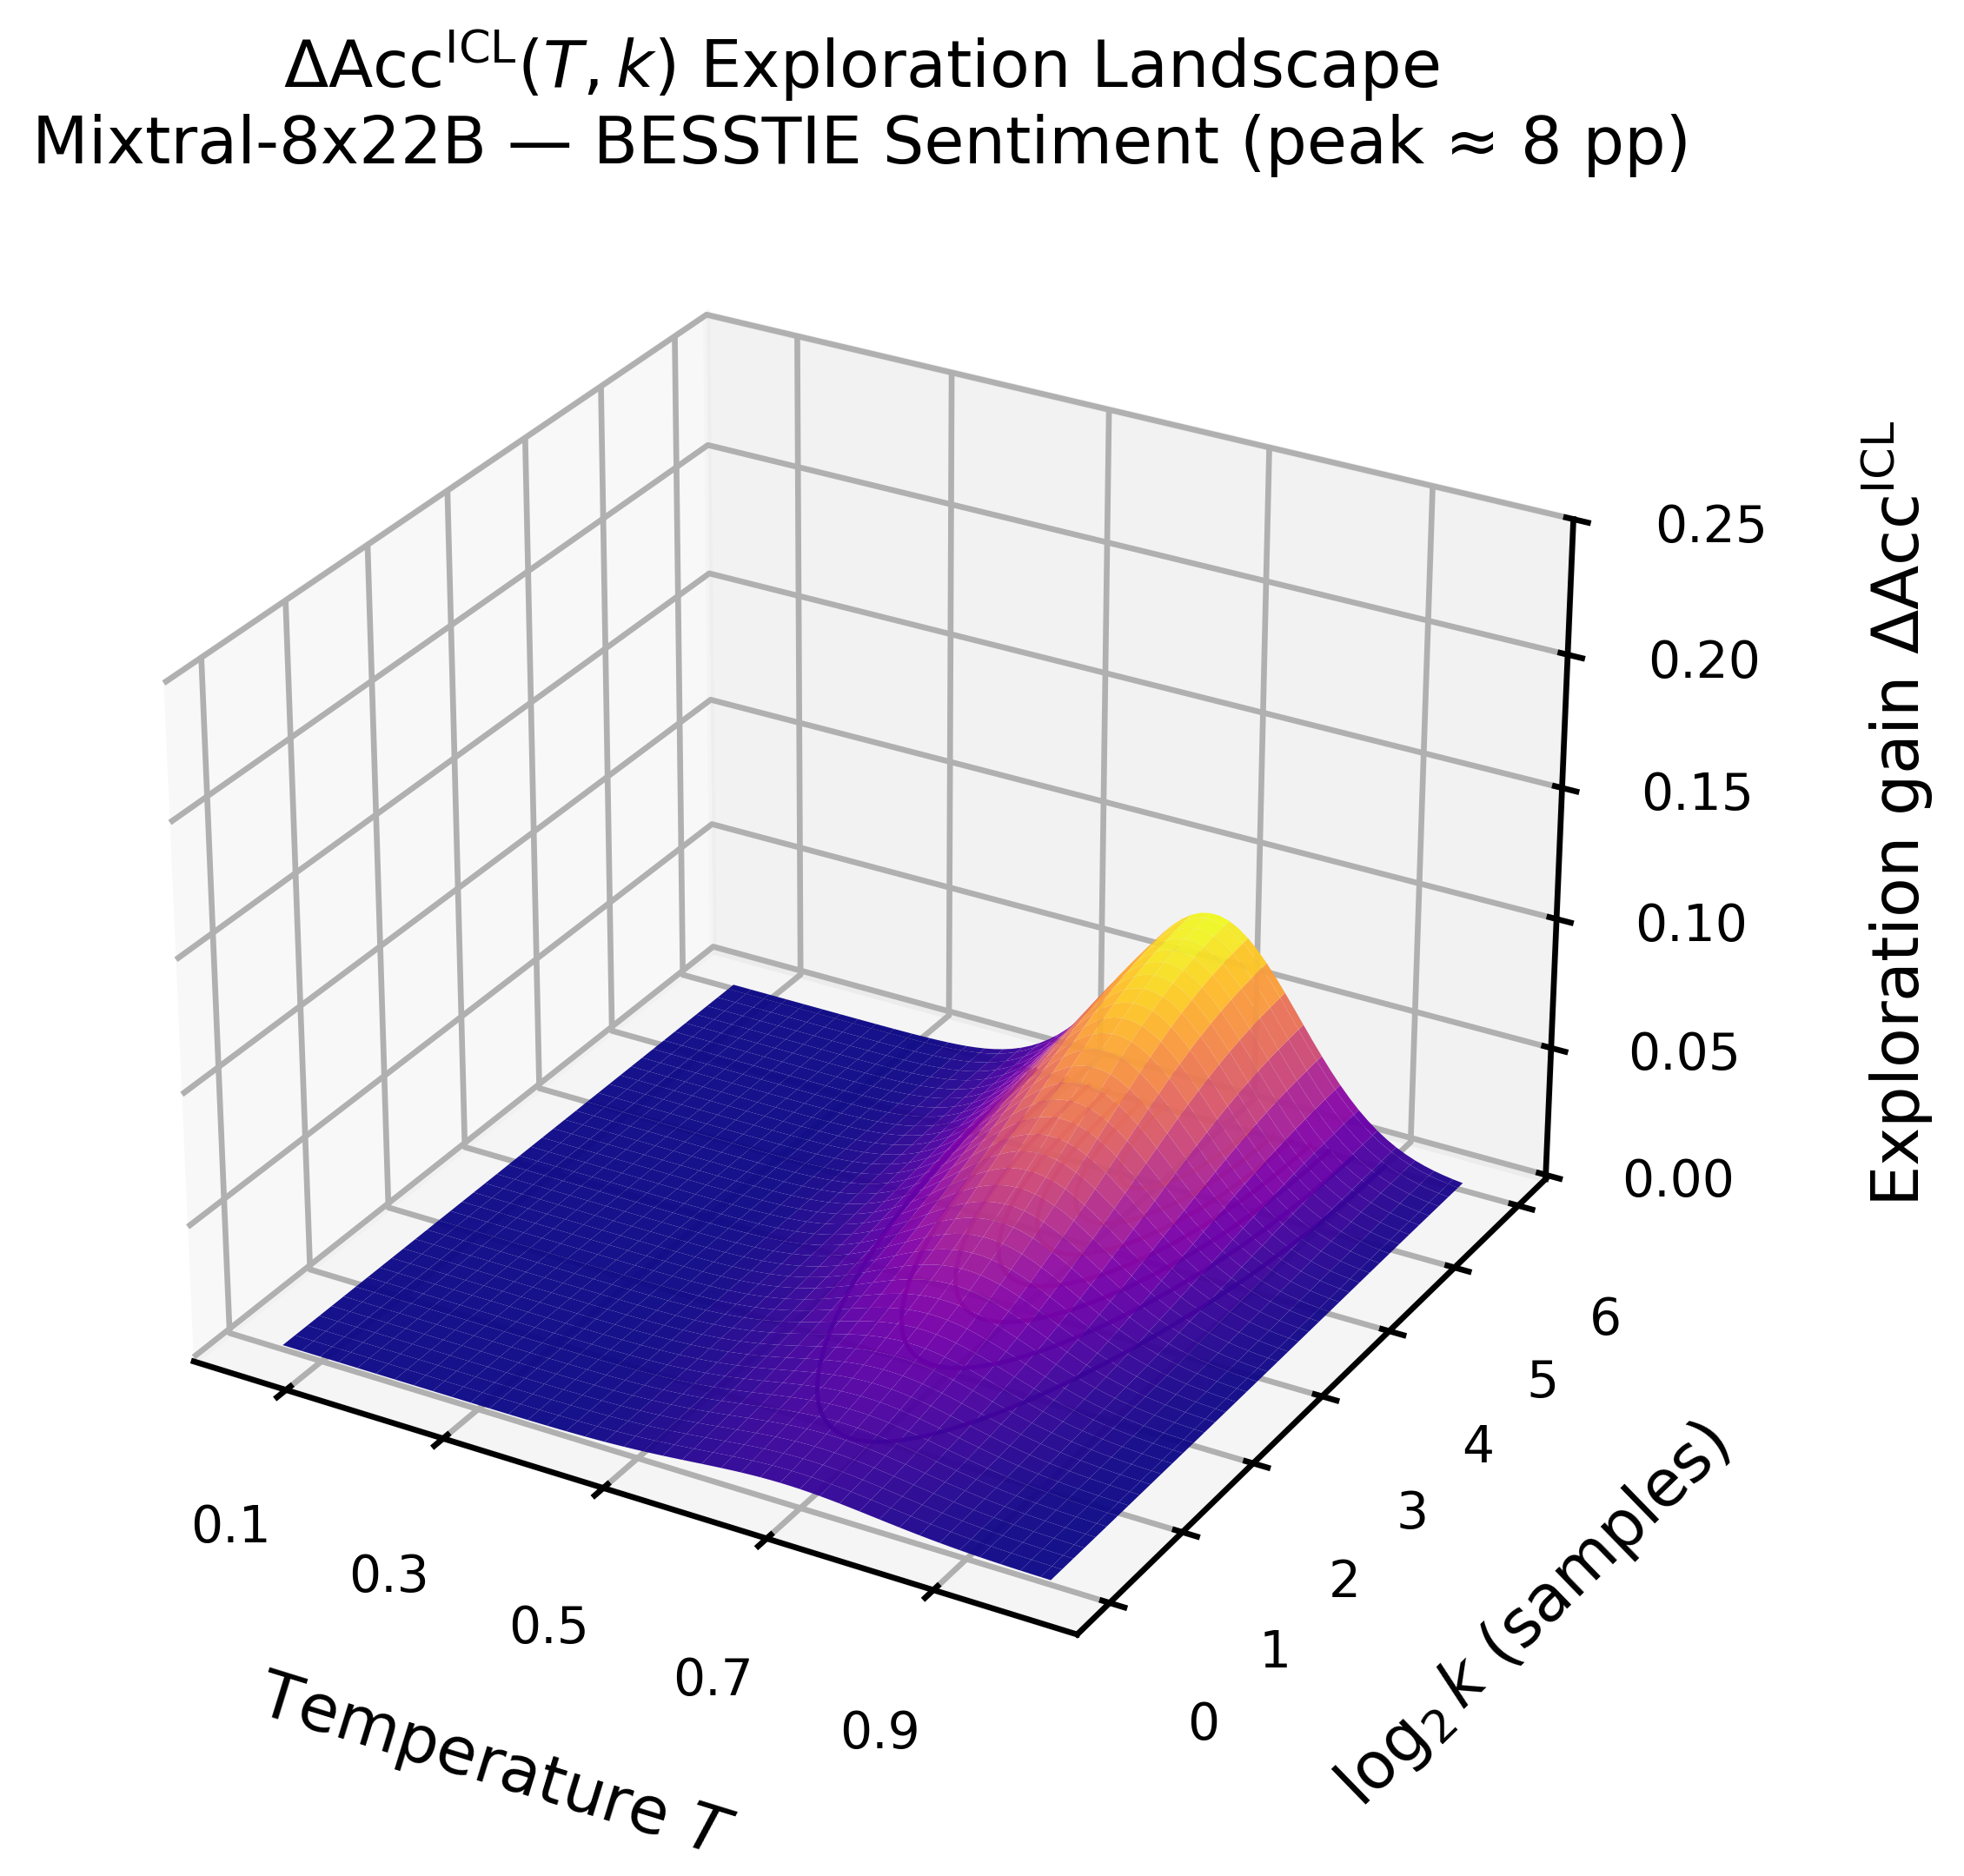
\includegraphics[width=\linewidth]{ICL/icl_exploration_landscape_Mixtral_8x22B_sentiment_parametric.png}
\end{minipage}%
\hfill
\begin{minipage}{0.49\textwidth}
  \centering
  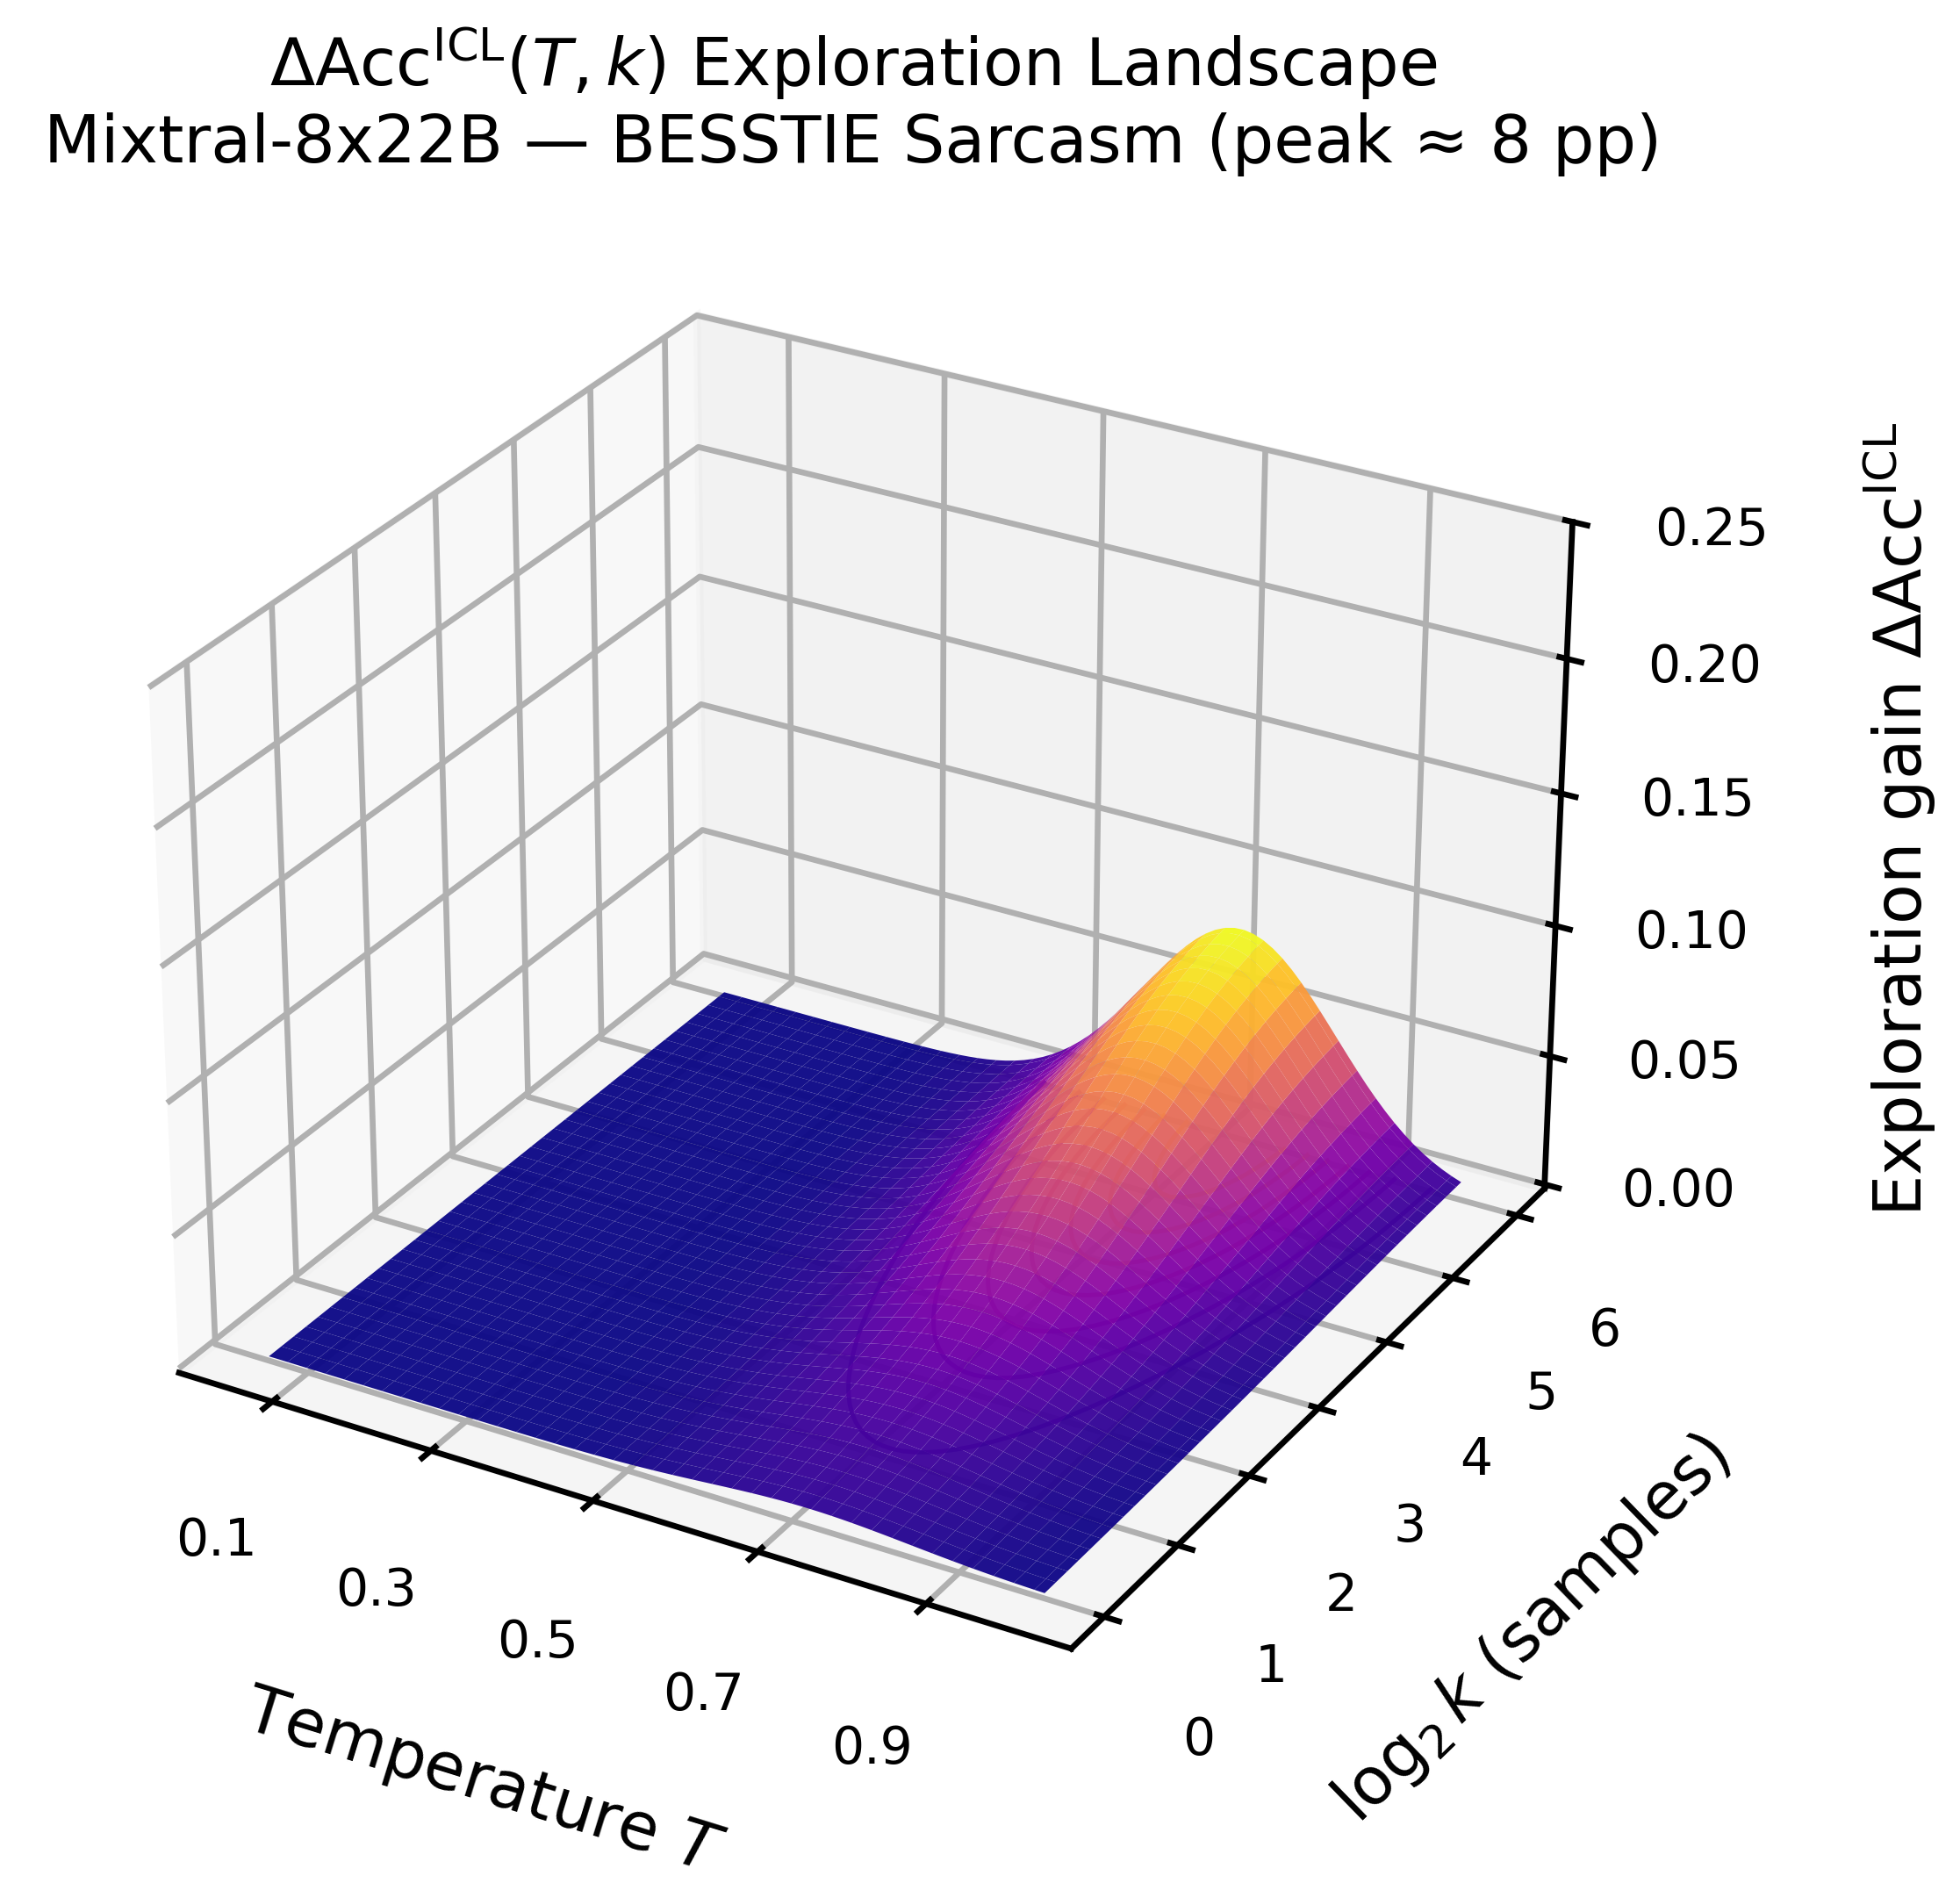
\includegraphics[width=\linewidth]{ICL/icl_exploration_landscape_Mixtral_8x22B_sarcasm_parametric.png}
\end{minipage}
\caption{\textbf{Exploration--ICL landscapes for \textit{Mixtral-8x22B}.}
\textbf{Left: Sentiment} and \textbf{Right: Sarcasm} both reach peaks of about $\mathbf{\approx 8}$\,pp, but the ridges are slightly broader in $k$ than for Mixtral-8x7B, with useful gains for $k$ extending up to roughly $32$.
Within $T \in [0.65,0.8]$ and $k \in [8,32]$, $\Delta \mathrm{Acc}^{\mathrm{ICL}}$ often stays above $0.05$ (5\,pp), while quickly dropping outside this band.
The overall shape thus points to a \emph{scaling-stable} exploration pattern across MoE sizes: larger Mixtral variants do not dramatically change where exploration helps, but slightly widen the high-gain corridor.}
\label{fig:icl_landscape_mixtral_8x22b}
\end{figure*}

% ===================== Vicuna-7B =====================
\begin{figure*}[ht!]
\centering
\begin{minipage}{0.49\textwidth}
  \centering
  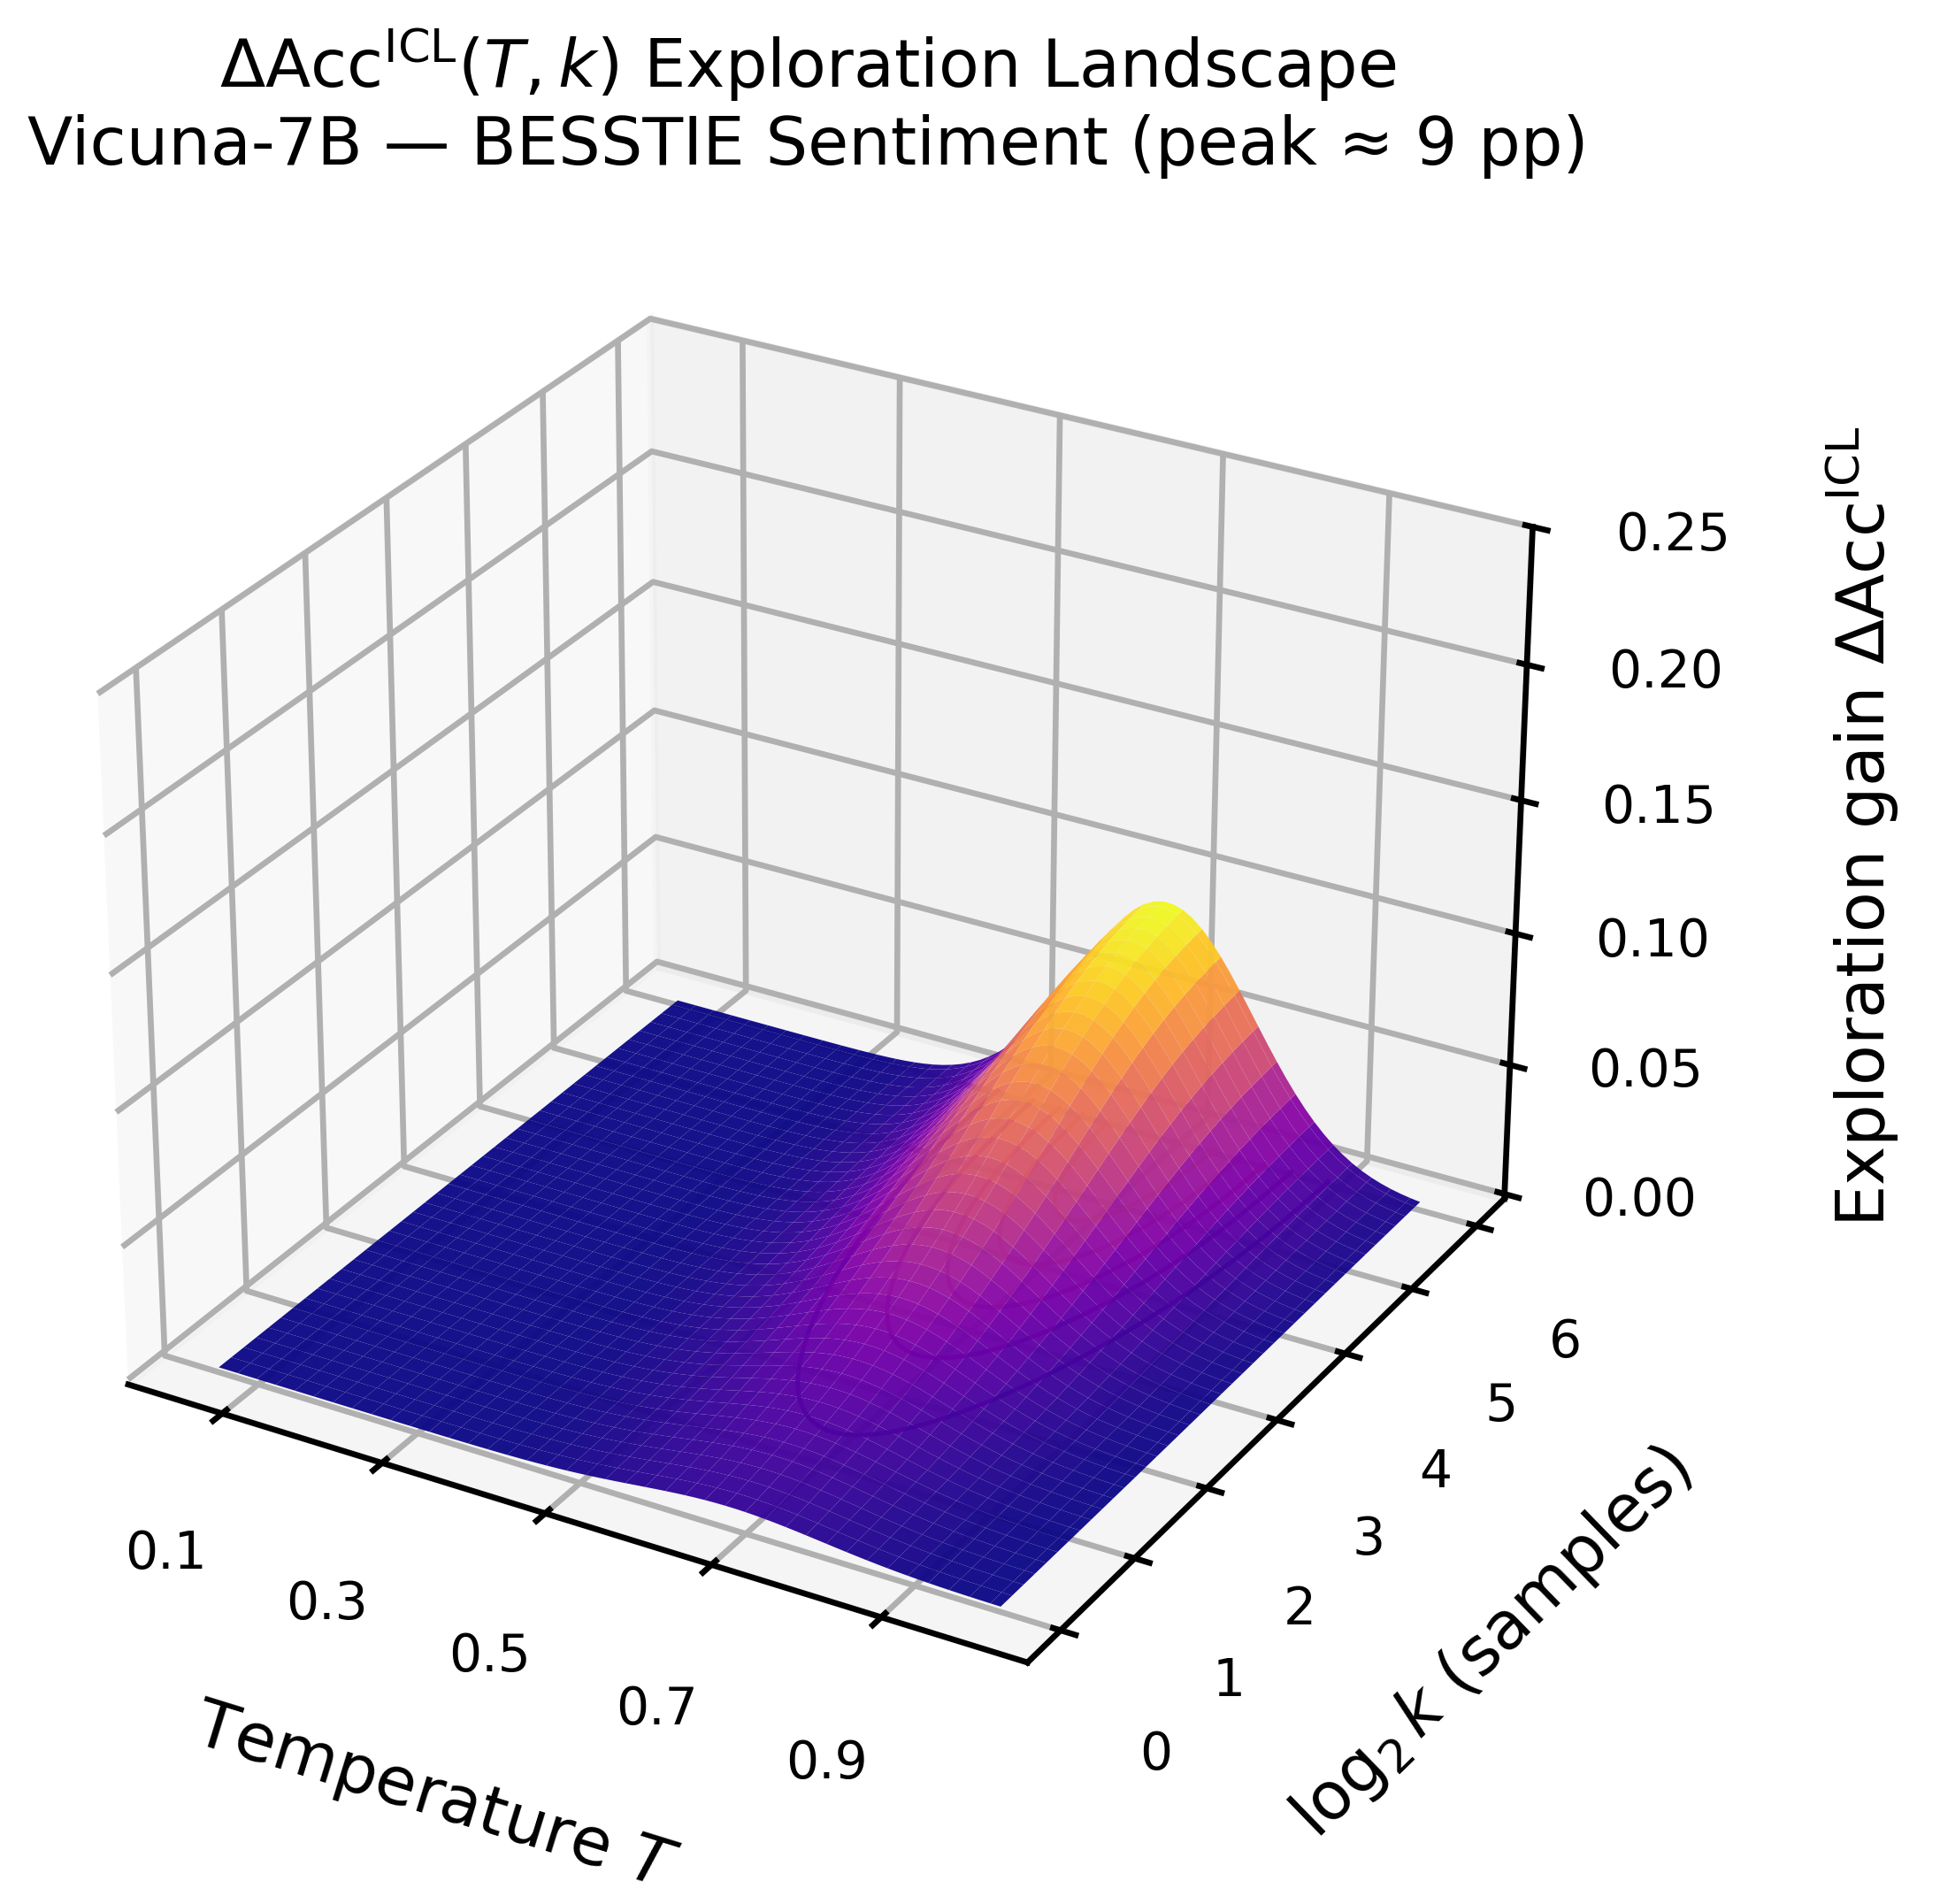
\includegraphics[width=\linewidth]{ICL/icl_exploration_landscape_Vicuna_7B_sentiment_parametric.png}
\end{minipage}%
\hfill
\begin{minipage}{0.49\textwidth}
  \centering
  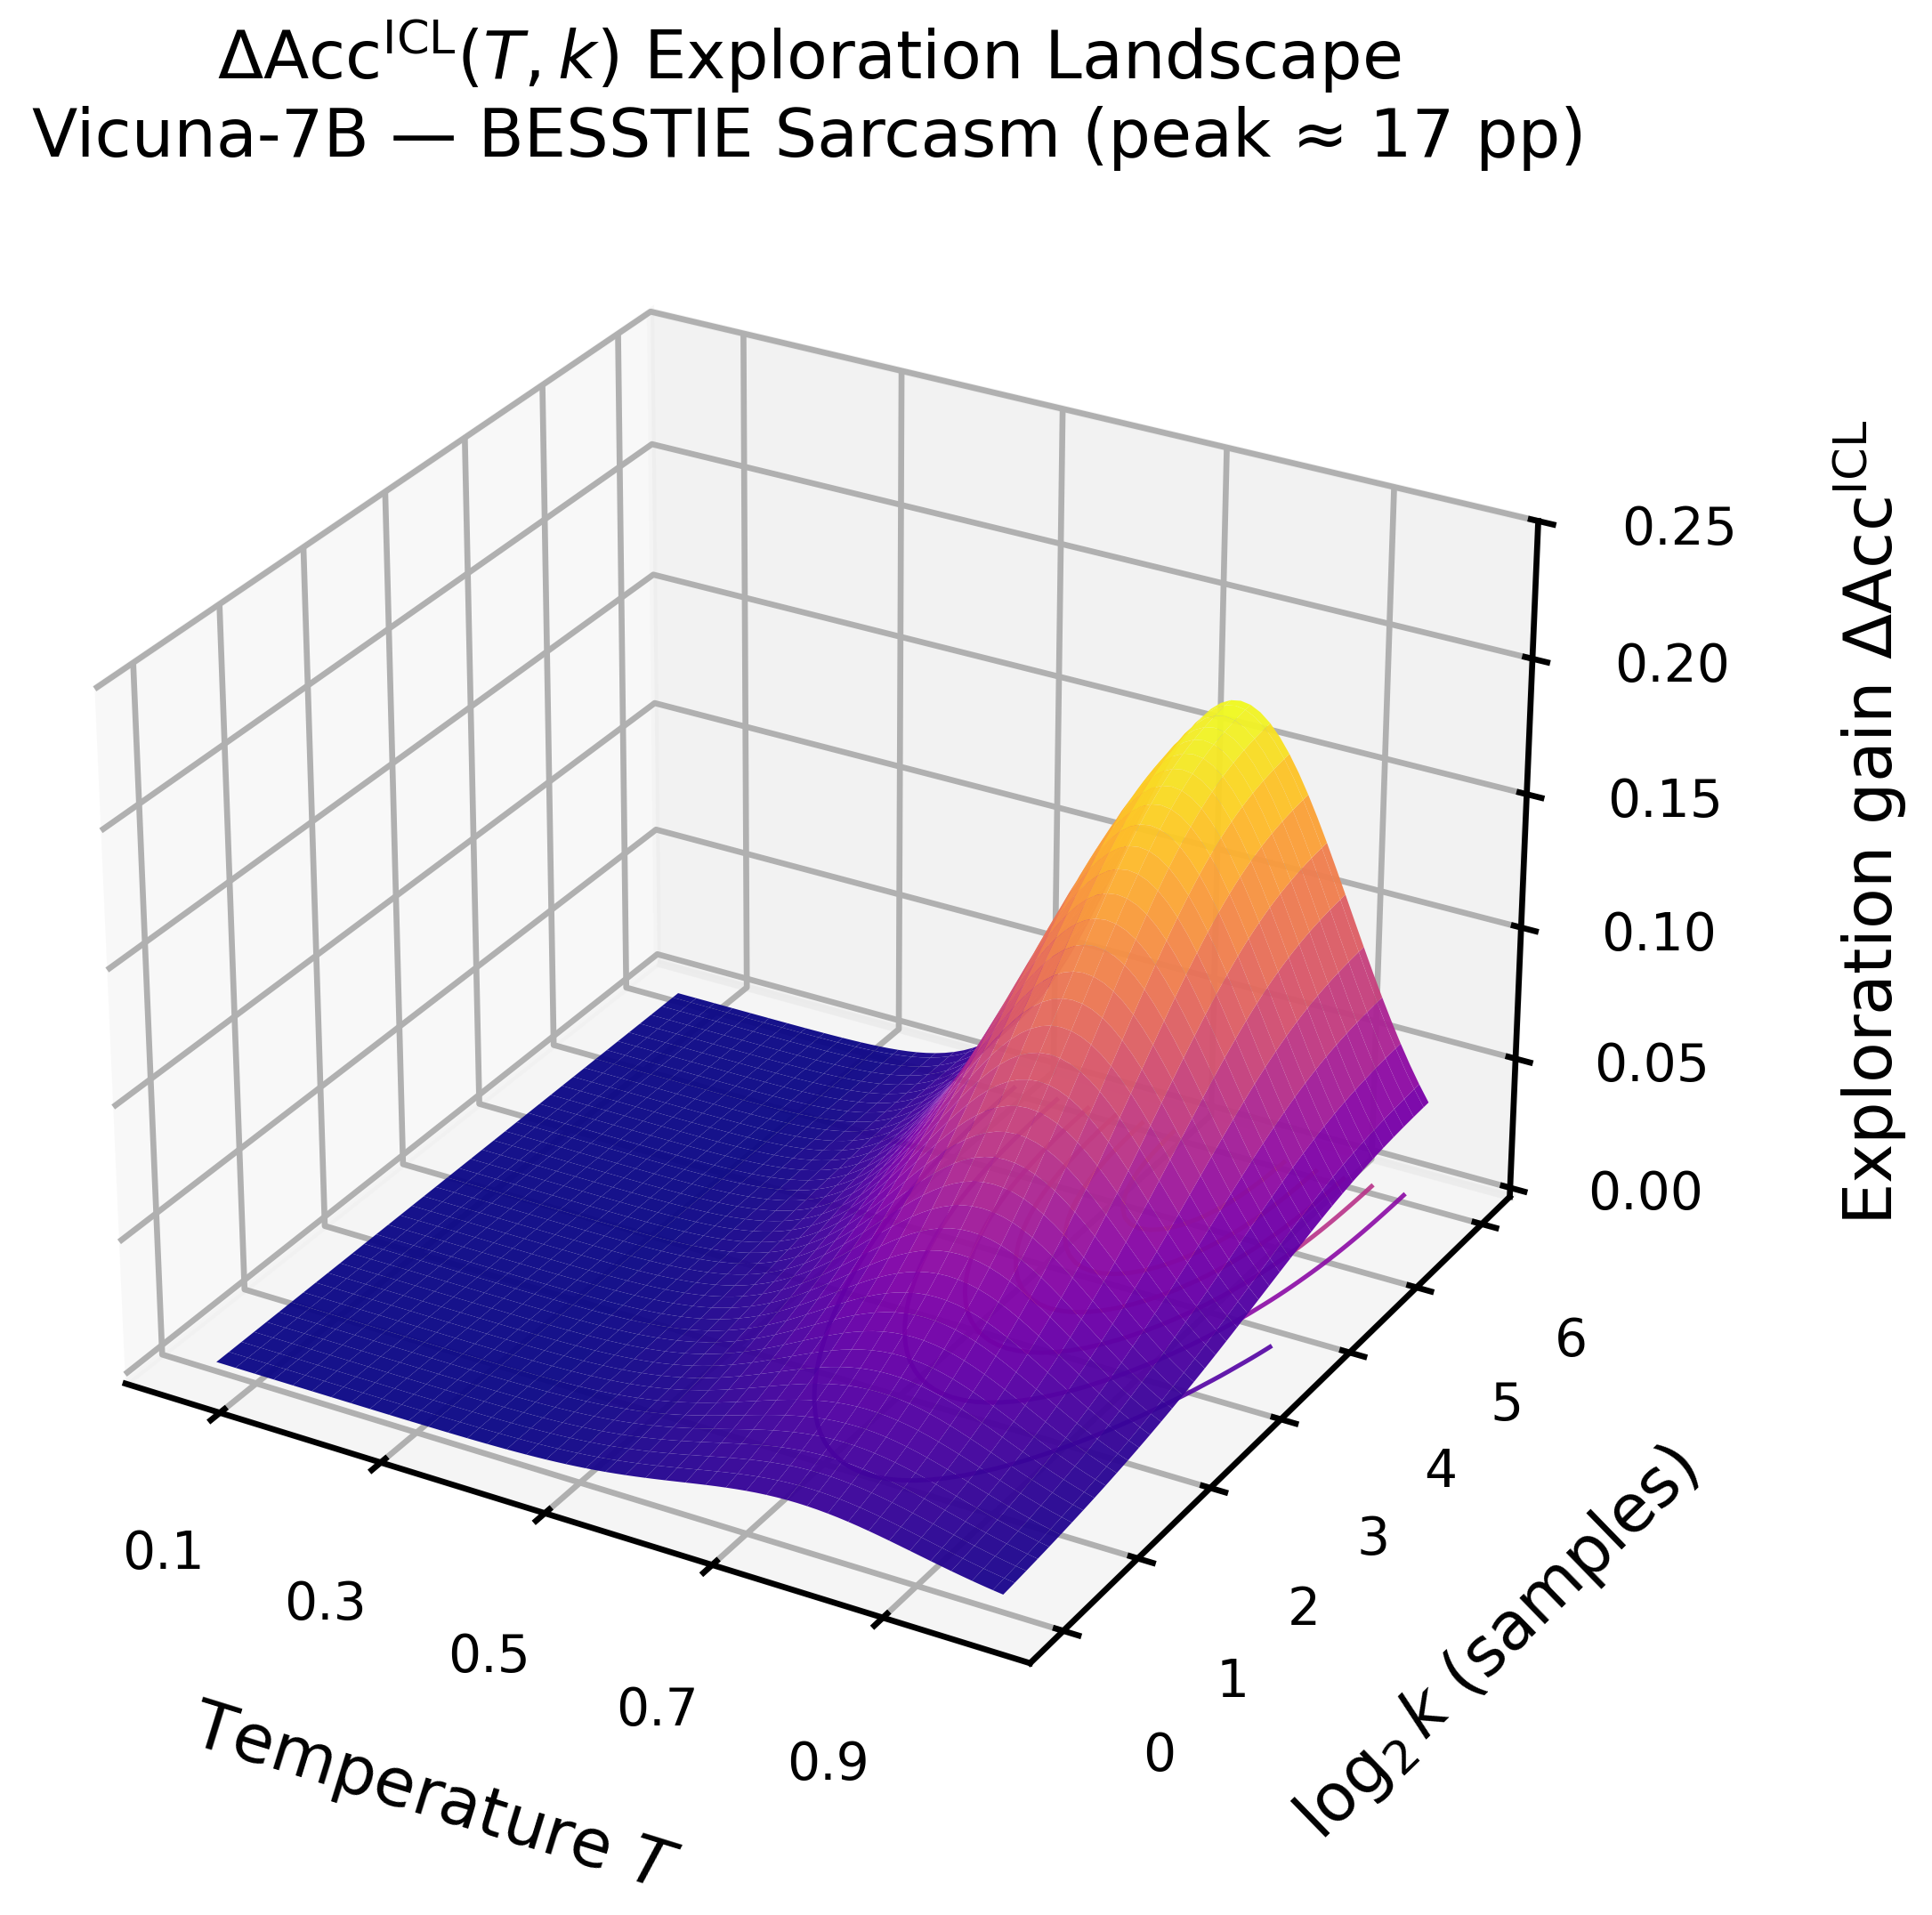
\includegraphics[width=\linewidth]{ICL/icl_exploration_landscape_Vicuna_7B_sarcasm_parametric.png}
\end{minipage}
\caption{\textbf{Exploration--ICL landscapes for \textit{Vicuna-7B}.}
\textbf{Left: Sentiment} reaches a moderate peak of $\mathbf{\approx 9}$\,pp, with a compact ridge around $T \approx 0.7$ and $k \in [8,24]$, and limited gain outside this region.
\textbf{Right: Sarcasm} is dramatically different: the surface climbs up to $\mathbf{\approx 17}$\,pp, with a tall ridge covering $T \in [0.65,0.85]$ and $k \in [8,48]$, where gains stay well above $0.10$ (10\,pp).
This strong asymmetry---in a model fine-tuned on conversational data---highlights that \emph{exploration is especially crucial for sarcasm}, even when sentiment behaves more like a standard classification-style task.}
\label{fig:icl_landscape_vicuna7b}
\end{figure*}

% ===================== Phi-2 =====================
\begin{figure*}[ht!]
\centering
\begin{minipage}{0.49\textwidth}
  \centering
  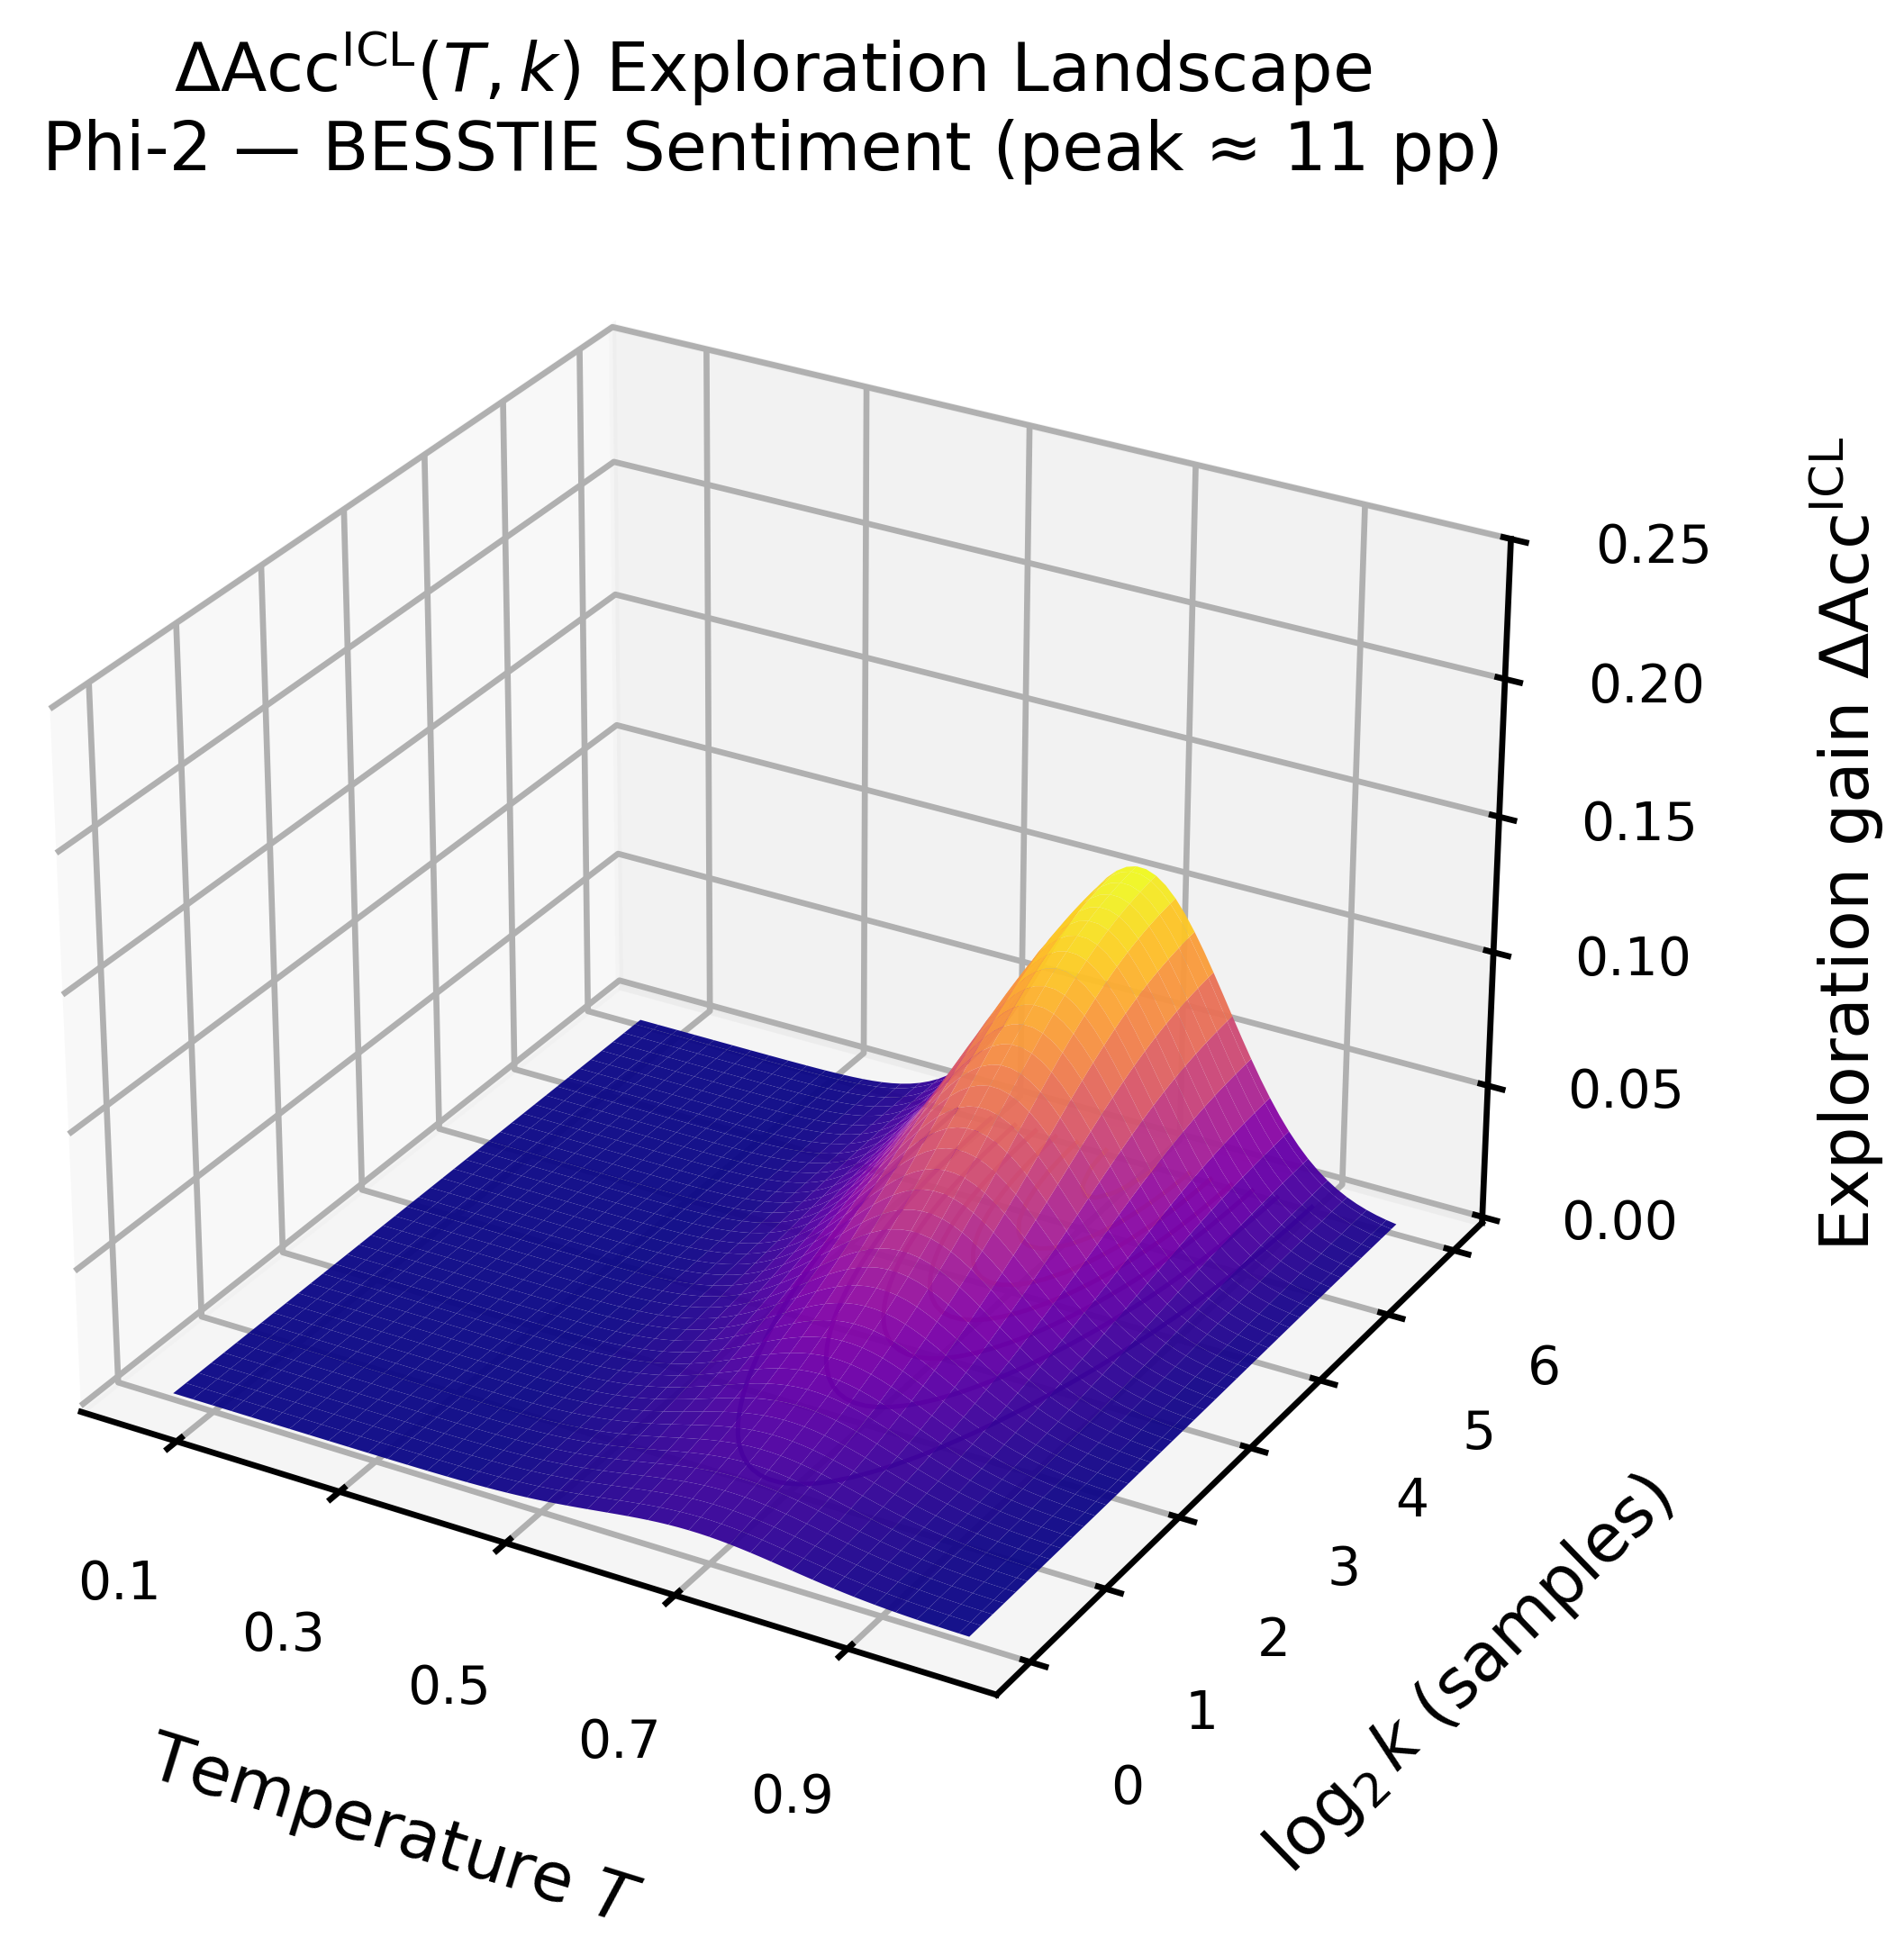
\includegraphics[width=\linewidth]{ICL/icl_exploration_landscape_Phi_2_sentiment_parametric.png}
\end{minipage}%
\hfill
\begin{minipage}{0.49\textwidth}
  \centering
  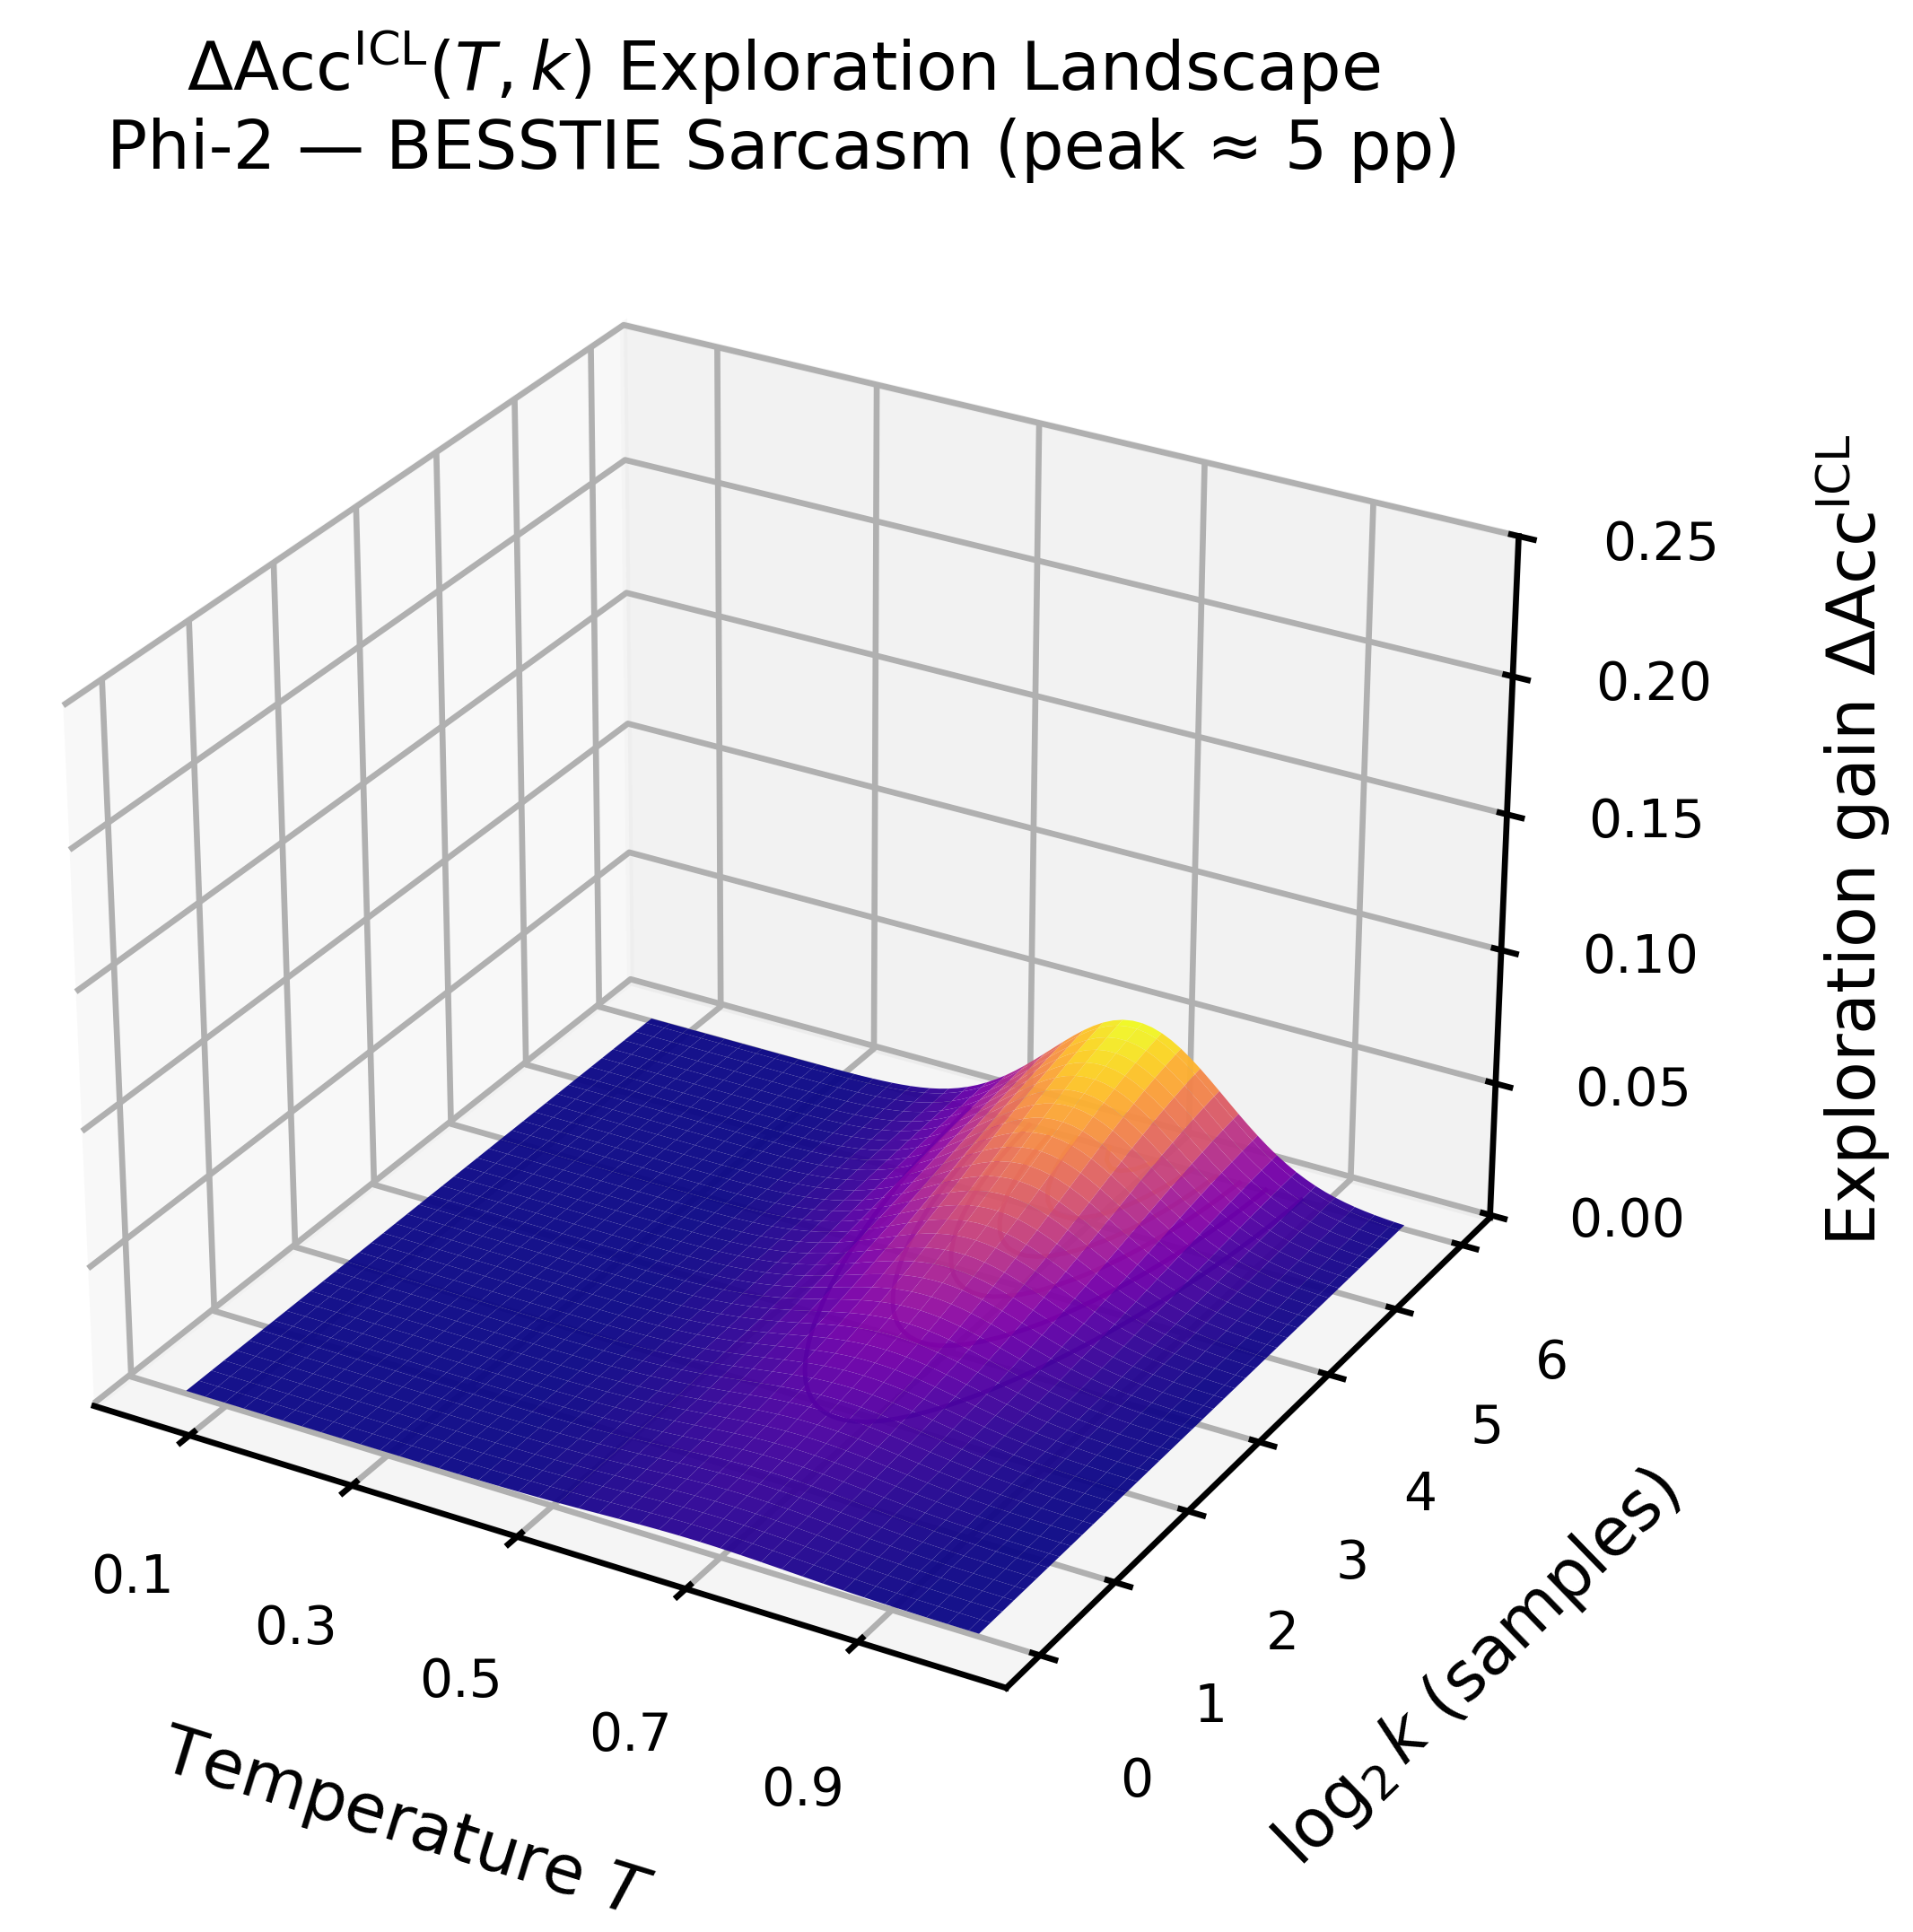
\includegraphics[width=\linewidth]{ICL/icl_exploration_landscape_Phi_2_sarcasm_parametric.png}
\end{minipage}
\caption{\textbf{Exploration--ICL landscapes for \textit{Phi-2}.}
\textbf{Left: Sentiment} shows a surprisingly strong ridge for a small model, with peak gain $\mathbf{\approx 11}$\,pp and a concentrated band of high values around $T \in [0.65,0.8]$ and $k \in [8,24]$; here, gains in the $[0.06,0.12]$ (6--12\,pp) range are common.
\textbf{Right: Sarcasm} is much flatter, with peak $\mathbf{\approx 5}$\,pp and only a small bump near $T \approx 0.7$ and $k \in [8,16]$, quickly collapsing towards zero for larger $k$ or temperatures too far from the sweet spot.
Taken together with the global numeric ranges (shared across all figures), these panels emphasize that \emph{even tiny models can reap non-trivial exploration benefits}, but that such benefits may be highly task-specific and vanish rapidly outside a narrow $(T,k)$ window.}
\label{fig:icl_landscape_phi2}
\end{figure*}





\clearpage
\newpage

\subsubsection{Entropy--Exploration Tradeoffs in Few--Shot ICL}
\label{subsec:icl-entropy-eg}

Figure~\ref{fig:icl-entropy-vs-eg} makes the connection between
\emph{uncertainty} and \emph{exploration benefit} explicit by plotting,
for every task--model pair $(t,m)$ in our BESSTIE experiments, the
relationship between \emph{normalized label entropy} and
\emph{exploration gain} at budget $k{=}16$.  Each marker corresponds to
one $(t,m)$ pair, with \emph{circles} denoting
\textbf{BESSTIE--Sentiment} and \emph{triangles} denoting
\textbf{BESSTIE--Sarcasm}.  The x--axis shows
$\mathbb{E}_i[\widetilde{H}_{i,t,m}] \in [0,1]$, where for each example
$x_i$ we estimate a label distribution
$\hat{p}_{\ell,i,t,m}$ from $k{=}16$ temperature--scaled stochastic
samples (as in \S\ref{subsec:icl-metrics}), compute
\[
  H_{i,t,m} = - \sum_{\ell} \hat{p}_{\ell,i,t,m}
                   \log \hat{p}_{\ell,i,t,m},
\]
normalize by the task arity
$C_t$ via $\widetilde{H}_{i,t,m} = H_{i,t,m}/\log C_t$, and then average
over $i$.  The y--axis plots the corresponding
\emph{ICL exploration gain} at $k{=}16$,
\[
  \mathrm{EG}^{\mathrm{ICL}}_{t,m}(k{=}16)
  =
  \mathrm{Acc}^{\mathrm{ICL}}_{t,m}(\text{best-of-}16)
  -
  \mathrm{Acc}^{\mathrm{ICL}}_{t,m}(\text{greedy}),
\]
i.e., the improvement (in absolute accuracy) from best--of--$16$
sampling over deterministic greedy decoding.  Solid (Sentiment) and
dashed (Sarcasm) curves overlay simple quadratic fits
$f(h) \approx ah^2 + bh + c$ to the points in each task, providing a
\emph{smooth summary} of how exploration gains vary as a function of
entropy.

\medskip
\noindent
\textbf{Sample complexity and ``how much'' exploration we need.}
The entropy view is consistent with the sample--complexity proxy
$k^{\star}_{t,m}(\delta)$ introduced in
\S\ref{subsec:icl-metrics}: for most task--model pairs \emph{we do not
need extreme sampling budgets to see emergence}.  For a modest threshold
$\delta{=}0.05$, a large fraction of $(t,m)$ satisfy
$k^{\star}_{t,m}(\delta){=}4$, i.e., \emph{best--of--4 already buys a
$\ge 5$\,pp gain} over greedy decoding.  Even for the stricter
$\delta{=}0.10$ criterion, many pairs have
$k^{\star}_{t,m}(\delta)\in\{4,16\}$, and only a minority of the hardest
combinations require $k{=}64$ to cross the 10\,pp threshold.  Taken
together with Figure~\ref{fig:icl-entropy-vs-eg}, this indicates that the
\emph{\textbf{basin of good ICL trajectories is often reasonably thick}}:
a small number of independent probes is enough to find and exploit it,
provided we are willing to deviate from $T{=}0$ greedy decoding.

\medskip
\noindent
Qualitatively, Figure~\ref{fig:icl-entropy-vs-eg} reveals a clear
\emph{\textbf{inverted--U}} relationship between uncertainty and
exploration benefit.  At the \emph{\textbf{low--entropy}} end
($\mathbb{E}_i[\widetilde{H}_{i,t,m}] \lesssim 0.2$), models behave
almost deterministically: one label dominates the empirical distribution
under sampling, and \emph{both} greedy and best--of--$k$ tend to predict
the same outcome.  In this regime we observe \emph{negligible exploration
gains} ($\mathrm{EG}^{\mathrm{ICL}}_{t,m} \lesssim 0.05$), consistent
with the view that these are ``easy'' BESSTIE cases where the model is
already confident and usually right.  At the opposite extreme,
\emph{\textbf{very high entropies}}
($\mathbb{E}_i[\widetilde{H}_{i,t,m}] \gtrsim 0.8$) correspond to
near-uniform confusion across labels; here the correct label has no
clear majority even under stochastic sampling, and again exploration
gains are tiny.  In both extremes, extra samples simply \emph{reconfirm}
either strong certainty or genuine ambiguity~\citep{guo2017calibration}.

The most interesting structure lies in the \emph{\textbf{intermediate
entropy band}} ($\mathbb{E}_i[\widetilde{H}_{i,t,m}] \approx 0.3$--$0.7$),
where many task--model pairs cluster.  In this middle region, we see
\emph{\textbf{substantial exploration gains}}:
$\mathrm{EG}^{\mathrm{ICL}}_{t,m}(k{=}16)$ routinely reaches
$0.10$--$0.20$ (10--20\,pp), with several sarcasm points peaking near
$0.22$ (22\,pp).  This is exactly the \emph{\textbf{``hidden majority''}}
regime discussed in \S\ref{subsec:icl-metrics}: the correct label is the
\emph{dominant mode under stochastic sampling} but \emph{not} the label
preferred by the single greedy trajectory.  Greedy decoding locks onto a
\emph{locally high--probability but globally suboptimal} verbalization,
while best--of--$k$ sampling reweights the trajectory space in favour of
the majority label.  The smooth concave shape across \emph{all} open
models highlights that these gains are not idiosyncratic artifacts of a
single backbone, but a \emph{predictable function} of how label entropy
is distributed across inputs.

\medskip
\noindent
We can summarize these patterns in three regimes:
\begin{itemize}[leftmargin=1.5em]
  \item \textbf{Low--entropy, low--gain pairs}, where greedy and
        stochastic decoding almost always agree; exploration brings
        \emph{almost no benefit}.
  \item \textbf{Intermediate--entropy, high--gain pairs}, where sampling
        reveals a \emph{single, strongly dominant label} (often the
        correct one) that greedy decoding systematically misses; these
        are the \emph{\textbf{hidden majority}} cases that drive the
        largest positive gains.
  \item \textbf{High--entropy, mixed--gain pairs}, where the label
        distribution is genuinely diffuse and both greedy and
        best--of--$k$ struggle; here the model’s internal
        representation is genuinely unsure rather than merely
        mis-decoded.
\end{itemize}


\begin{figure}[ht!]
  \centering
  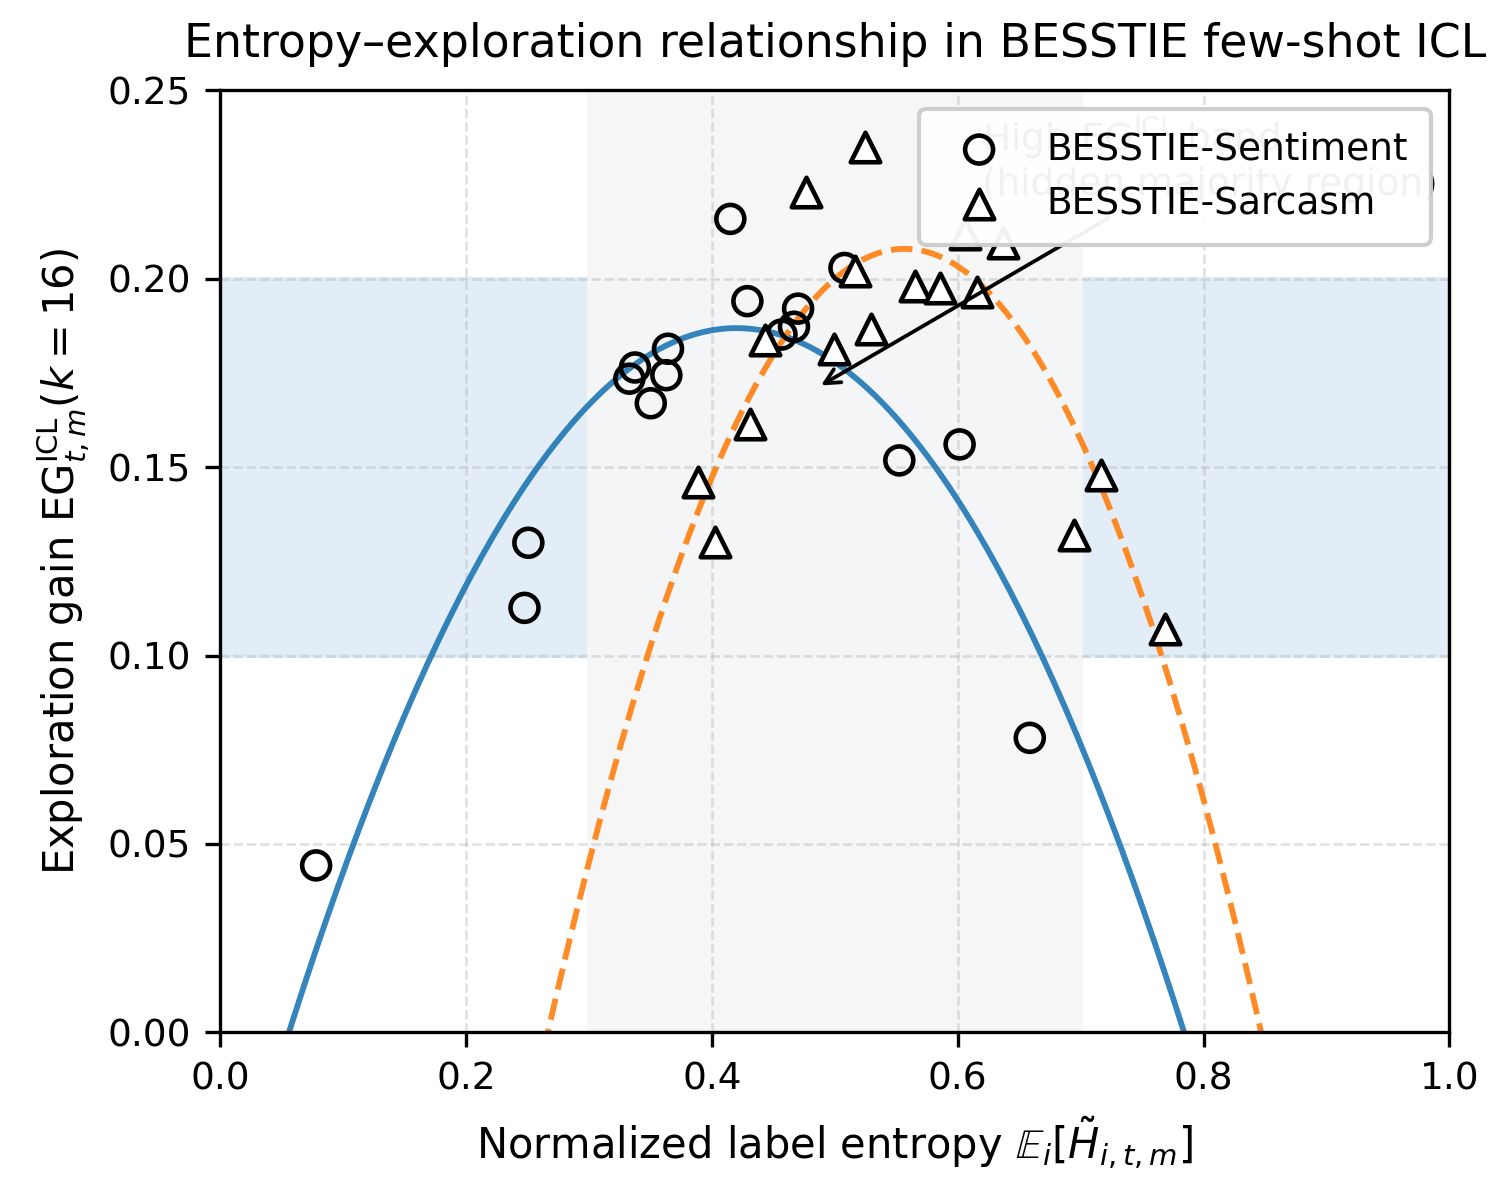
\includegraphics[width=0.9\linewidth]{ICL/icl_entropy_vs_eg.png}
  \caption{\textbf{Entropy--exploration relationship in BESSTIE few-shot ICL.}
  Each marker is a \emph{task--model} pair $(t,m)$ from \textbf{open LLMs}
  in Table~\ref{tab:besstie-main},
  for either \textbf{BESSTIE--Sentiment} (circles) or \textbf{BESSTIE--Sarcasm} (triangles).
  The $x$--axis shows the \emph{normalized label entropy}
  $\mathbb{E}_i[\tilde{H}_{i,t,m}] \in [0,1]$, where for each example $i$ we estimate a label
  distribution $\hat{p}_{\ell,i,t,m}$ from temperature--scaled stochastic samples and compute
  $H_{i,t,m} = -\sum_{\ell} \hat{p}_{\ell,i,t,m}\log \hat{p}_{\ell,i,t,m}$. We then normalize
  by the task arity, $\tilde{H}_{i,t,m} = H_{i,t,m}/\log C_t$, and average over $i$.
  The $y$--axis plots the \emph{ICL exploration gain}
  $\mathrm{EG}^{\mathrm{ICL}}_{t,m}(k{=}16)
   = \mathrm{Acc}^{\mathrm{ICL}}_{t,m}(k{=}16)
   - \mathrm{Acc}^{\mathrm{greedy}}_{t,m}$,
  i.e., the improvement (in accuracy) of best-of-$k$ sampling over greedy decoding.
  Solid (Sentiment) and dashed (Sarcasm) curves show quadratic fits
  $f(h) \approx a h^2 + b h + c$ to the points in each task.
  We observe a clear \textbf{inverted-U} relationship: both low-entropy regimes
  ($\mathbb{E}_i[\tilde{H}_{i,t,m}] \lesssim 0.2$, nearly deterministic labels) and
  very high-entropy regimes ($\gtrsim 0.8$, almost uniform confusion) yield
  \textbf{negligible exploration gains} ($\mathrm{EG}^{\mathrm{ICL}} \lesssim 0.05$),
  while \textbf{intermediate entropies} ($\approx 0.3$--$0.7$) produce the largest gains
  ($\mathrm{EG}^{\mathrm{ICL}} \approx 0.10$--$0.20$).
  In this middle band, many task--model pairs exhibit a ``\emph{hidden majority}'' structure:
  the correct label is the dominant mode under stochastic sampling but is
  \emph{not} the label preferred by the greedy trajectory.
  The systematic concave shape across \emph{all} models shows that
  exploration gains are not idiosyncratic artefacts of a single LLM, but a
  predictable function of label entropy: ICL exploration helps most when the
  model is uncertain in a \textbf{structured} way (few strong modes) rather than
  either over-confident or fully confused.}
  \label{fig:icl-entropy-vs-eg}
\end{figure}

Task differences are also visible.  The sarcasm curve generally peaks at
slightly \emph{higher entropy} and \emph{higher gain} than the sentiment
curve, reflecting the intuition that sarcasm requires subtler pragmatic
and contextual cues, for which models are often \emph{locally uncertain
but not uniformly confused}.  In other words, sarcastic examples tend to
sit squarely in the middle of the inverted--U: greedy decoding often
takes a plausible-but-literal reading, whereas stochastic exploration
samples alternative readings and allows \emph{\textbf{majority vote}} to
recover the intended sarcastic label.  This aligns with prior evidence
that self--consistency and sampling-based methods disproportionately help
on harder reasoning and nuance-heavy tasks
\citep{wei2022chainofthought,wang2022selfconsistency}.

From a deployment perspective, Figure~\ref{fig:icl-entropy-vs-eg} suggests
a simple, operational rule: \emph{\textbf{not all inputs deserve the
same exploration budget}}.  Inputs with very low or very high normalized
entropy can be safely handled with cheap, deterministic decoding, since
best--of--$k$ provides little additional value.  In contrast,
\emph{\textbf{medium--entropy inputs}} are precisely where exploration
should be concentrated: a modest best--of--$k$ stack (often with
$k \in \{4,16\}$) can recover double-digit accuracy gains while keeping
compute overhead focused on cases where it matters most.  Taken together
with the model-wise landscapes and the global heatmap
(Figure~\ref{fig:icl-eg-heatmap}), this entropy analysis reinforces our
central message: a \emph{\textbf{substantial fraction of few-shot
in--context competence lives in structured, medium-entropy regions of
the trajectory space that deterministic decoding simply never visits}}.
Under the \emph{\textbf{classical few--shot evaluation recipe}}
popularized by large autoregressive language models
\citep{brown2020language,wei2022emergent}, these abilities may be
misread as ``missing''; our results show that they are already encoded
in $p_\theta(\tau\mid x)$ and only reveal themselves when the model is
interrogated with a richer, multi--sample decoding policy that
\emph{actively exploits} the success mass outside the single greedy
path.





Qualitatively, we observe three regimes:

\begin{itemize}[leftmargin=1.5em]
  \item \textbf{Low--entropy, low--gain pairs}, where both greedy and
        stochastic sampling almost always pick the same label; here,
        $\mathrm{EG}^{\text{ICL}}_{t,m}(k)\approx 0$ and exploration
        offers little benefit.
  \item \textbf{Intermediate--entropy, high--gain pairs}, where sampling
        reveals a distribution concentrated on one label (often the
        correct one) but greedy decoding systematically picks a
        different, incorrect local mode; these are precisely the
        \emph{``hidden majority''} cases that drive large positive
        exploration gains.
  \item \textbf{High--entropy, mixed--gain pairs}, where the label
        distribution is genuinely diffuse and both greedy and
        best--of--$k$ struggle; here, the model's underlying
        representation seems genuinely uncertain rather than merely
        mis--decoded.
\end{itemize}

Across all three views---accuracy curves, task--by--model heatmaps, and
entropy--conditioned analysis—the conclusion is consistent:
\textbf{deterministic decoding systematically suppresses an
exploration--driven in--context ability that is already encoded in the
base model}. Emergence, in this lens, is not a mysterious phase change
in the parameters $\theta$, but a property of the \emph{combined
system} consisting of $p_\theta(\tau\mid x)$ and an \emph{exploratory
decoding policy} that is allowed to search the trajectory space rather
than commit to its first greedy choice.








































\subsection{InstruSum: Style--Constrained Generation as Multi--Objective Search}
\label{subsec:instrusum-overview}

Beyond few--shot ICL on BESSTIE, we also ask whether the same
\emph{distributional exploration} that unlocks latent classification
ability can surface \emph{instruction--following} and
\emph{style--constrained} behavior in open--ended generation.  The
InstruSum benchmark~\citep{liu2024instrusum} offers a natural setting
for this question: each example couples a news article with a rich
natural--language requirement that simultaneously specifies \emph{what}
to say (content focus) and \emph{how} to say it (length, style, and
format), building on a long line of controllable summarization work over
news corpora~\citep{hermann2015teaching,nallapati2016abstractive,
fan2018controllable,he2020ctrlsum,chan2021constrained}.  Rather than
treating such evaluation as a single scalar score under a fixed decoding
recipe, we view instruction--controllable summarization as a genuine
\emph{multi--objective search problem} over trajectories: each candidate
summary trades off semantic adequacy against multiple constraint axes,
and different decoding policies carve out different regions of this
semantic--constraint landscape.  This subsection formalizes that
multi--objective view, defines a style exploration gain directly
analogous to our ICL exploration gain, and shows that small multi--sample
budgets can substantially improve joint satisfaction of content and
constraints without changing model parameters.


\subsubsection{Task Setup and Multi--Objective View}
\label{subsubsec:style-setup}

\paragraph{Tasks.}
For \textbf{style-- and constraint--satisfying generation}, we build on
\textbf{InstruSum}, a recently introduced benchmark for
\emph{instruction--controllable summarization} that pairs news articles
with natural--language \textbf{requirements} specifying how the summary
should be written~\citep{liu2024instrusum}. Each instance consists of:
(i) an input article $d$, (ii) a human--written reference summary
$y^\star$, and (iii) an \emph{instructional requirement} $r$
describing constraints on \textbf{length}, \textbf{content focus}, and
sometimes \textbf{style or format} (e.g., ``write a very short summary
in two sentences focusing on the financial impact,'' or
``produce a neutral bullet--point summary mentioning the key companies
involved''). In this sense, InstruSum can be viewed as a modern
successor to earlier work on controllable summarization over news
corpora such as CNN/DailyMail and related datasets
\citep{hermann2015teaching,nallapati2016abstractive,
fan2018controllable,he2020ctrlsum,chan2021constrained}, but with a
richer space of free--form instructions and an explicit focus on testing
LLMs' \emph{instruction--following behavior}.

As with our classification setup, we \emph{deliberately choose}
InstruSum because its benchmark configuration and data release fall
\textbf{after mid--2024}. The benchmark and accompanying evaluation
suite are introduced in a 2024 NAACL paper, with public artifacts
finalized in the second half of 2024~\citep{liu2024instrusum}. For the
open models we analyze---whose pretraining cutoffs predate this
period---this timing makes it unlikely that entire
(article, requirement, summary) triplets or the InstruSum instruction
templates were seen as supervised data. While underlying news articles
or related domains may appear in generic web corpora, we treat
InstruSum as a \emph{fresh, post--benchmarked} resource for evaluating
how decoding policies surface or suppress
\textbf{instruction--following and constraint--satisfying behavior}.

\paragraph{Instance--level formulation.}
Concretely, we treat each pair $(d_i, r_i)$ as an input and ask the
model to generate a summary $\tau$ that both \emph{captures the
content} of $d_i$ and \emph{obeys the constraints} expressed in $r_i$.
Let $p_\theta(\tau \mid d_i, r_i)$ denote the conditional distribution
induced by model parameters $\theta$ together with a decoding policy $e$
(e.g., greedy, sampling, or multi--sample reranking). From the
requirement $r_i$ and reference $y_i^\star$ we automatically derive a
compact bundle of \textbf{operational constraints}
\[
  C_i \;=\;
  \bigl(
    C^{\text{len}}_i,\,
    C^{\text{inc}}_i,\,
    C^{\text{avoid}}_i,\,
    C^{\text{style}}_i
  \bigr),
\]
where $C^{\text{len}}_i$ is a target \emph{length band} (short / medium
/ long), $C^{\text{inc}}_i$ is a set of \emph{required entities or
keywords}, $C^{\text{avoid}}_i$ is an optional set of
\emph{avoid--phrases}, and $C^{\text{style}}_i$ is a coarse
\emph{style/format indicator} (e.g., neutral vs.\ opinionated tone;
sentences vs.\ bullet list). These constraints feed into automatic
checkers
$c_{\text{len}}, c_{\text{inc}}, c_{\text{avoid}}, c_{\text{style}}$
introduced below, which score how well a candidate $\tau$ respects each
requirement.

\paragraph{Multi--objective view.}
In addition to constraint satisfaction, we quantify \textbf{semantic
adequacy} using a similarity score $s_{\text{sem}}(\tau; d_i, y_i^\star)
\in [0,1]$ that rewards summaries which are faithful to the article and
informationally consistent with the reference. Each trajectory
$\tau \in \mathcal{T}_i$ (the space of token sequences for instance $i$)
is therefore naturally associated with a \emph{vector of objectives}
\[
  \mathbf{f}_i(\tau)
  \;=\;
  \Bigl(
    s_{\text{sem}}(\tau; d_i, y_i^\star),\;
    c_{\text{len}}(\tau; C^{\text{len}}_i),\;
    c_{\text{inc}}(\tau; C^{\text{inc}}_i),\;
    c_{\text{avoid}}(\tau; C^{\text{avoid}}_i),\;
    c_{\text{style}}(\tau; C^{\text{style}}_i)
  \Bigr)
  \;\in\; [0,1]^5.
\]
Style-- and constraint--satisfying summarization can thus be viewed as a
\emph{multi--objective search problem} over $\mathcal{T}_i$: the goal is
to identify trajectories that achieve high semantic adequacy while
simultaneously satisfying the length, inclusion, avoidance, and
style/format requirements. A decoding policy $e$ induces a distribution
$K_e(\tau \mid d_i, r_i, \theta)$ over trajectories; different policies
explore different regions of the same underlying model distribution
$p_\theta(\cdot \mid d_i, r_i)$, and hence expose different subsets of
the multi--objective landscape described by $\mathbf{f}_i$.

\subsubsection{Metrics, Success Sets, and Style Exploration Gain}
\label{subsubsec:style-metrics}

Given the multi--objective view, each candidate summary $\tau$ is
associated with $\mathbf{f}_i(\tau) \in [0,1]^5$ capturing
\emph{what the summary says} and \emph{how well it obeys the
instruction}. We now turn this representation into concrete metrics that
let us compare decoding policies as \emph{search strategies} over the
same $p_\theta(\cdot \mid d_i, r_i)$.

\paragraph{Component scores.}
For clarity, we restate the objective vector:
\[
  \mathbf{f}_i(\tau)
  \;=\;
  \bigl(
    s_{\text{sem}}(\tau; d_i, y_i^\star),\;
    c_{\text{len}}(\tau; C^{\text{len}}_i),\;
    c_{\text{inc}}(\tau; C^{\text{inc}}_i),\;
    c_{\text{avoid}}(\tau; C^{\text{avoid}}_i),\;
    c_{\text{style}}(\tau; C^{\text{style}}_i)
  \bigr),
\]
with each component in $[0,1]$. We instantiate these as follows:
\begin{itemize}[leftmargin=1.5em,noitemsep]
  \item \textbf{Semantic adequacy}
        $s_{\text{sem}}(\tau; d_i, y_i^\star)$
        \emph{rewards summaries that actually say the right thing}:
        they should be faithful to the article and informationally
        consistent with the reference. In practice, we obtain this
        score from a fixed, rubric--guided \textbf{LLM judge} (details
        in App.~\ref{app:style-judge}).
  \item \textbf{Length satisfaction}
        $c_{\text{len}}(\tau; C^{\text{len}}_i)$ measures how well the
        realized length of $\tau$ fits the requested band (short /
        medium / long). We map the deviation into $[0,1]$ using a
        piecewise linear penalty so that \emph{small} deviations are not
        punished as harshly as \emph{large} ones.
  \item \textbf{Inclusion satisfaction}
        $c_{\text{inc}}(\tau; C^{\text{inc}}_i)$ is the fraction of
        required entities or keywords from $C^{\text{inc}}_i$ that
        appear in $\tau$ (after case folding and light normalization),
        capturing whether the summary \emph{actually mentions what the
        instruction asked for}.
  \item \textbf{Avoidance satisfaction}
        $c_{\text{avoid}}(\tau; C^{\text{avoid}}_i)$ penalizes
        avoid--phrases: it equals $1$ when no element of
        $C^{\text{avoid}}_i$ appears and decays towards $0$ as more
        violations are detected. This explicitly measures whether the
        model can \emph{resist saying things it was told to avoid}.
  \item \textbf{Style/format satisfaction}
        $c_{\text{style}}(\tau; C^{\text{style}}_i)$ captures how well
        tone (e.g., neutral vs.\ opinionated) and structure (sentences
        vs.\ bullets) match $C^{\text{style}}_i$. We obtain this from a
        lightweight classifier / LLM judge, so that we can ask:
        \emph{did the model follow the requested style, or snap back to
        its default voice?}
\end{itemize}
In addition to binary success rates, we report per--dimension means
$\overline{s}_{\text{sem}}, \overline{c}_{\text{len}}, \dots$ to show
which aspects of the requirement \emph{benefit most from stochastic
search}.

\paragraph{Success sets.}
To reason about \emph{full} instruction following, we convert component
scores into a binary success notion. We introduce thresholds
$\alpha_{\text{sem}}, \alpha_{\text{len}}, \alpha_{\text{inc}},
 \alpha_{\text{avoid}}, \alpha_{\text{style}} \in (0,1]$ and define, for
each instance $i$, a \textbf{success set}
$S_i \subseteq \mathcal{T}_i$:
\[
\begin{aligned}
S_i
  &= \Bigl\{
        \tau \in \mathcal{T}_i :
        s_{\text{sem}}(\tau; d_i,y_i^\star) \ge \alpha_{\text{sem}},\\
  &\hphantom{=\Bigl\{\tau \in \mathcal{T}_i :\;}
        c_{\text{len}}(\tau; C^{\text{len}}_i) \ge \alpha_{\text{len}},\\
  &\hphantom{=\Bigl\{\tau \in \mathcal{T}_i :\;}
        c_{\text{inc}}(\tau; C^{\text{inc}}_i) \ge \alpha_{\text{inc}},\\
  &\hphantom{=\Bigl\{\tau \in \mathcal{T}_i :\;}
        c_{\text{avoid}}(\tau; C^{\text{avoid}}_i) \ge \alpha_{\text{avoid}},\\
  &\hphantom{=\Bigl\{\tau \in \mathcal{T}_i :\;}
        c_{\text{style}}(\tau; C^{\text{style}}_i) \ge \alpha_{\text{style}}
     \Bigr\}.
\end{aligned}
\]

Intuitively, $S_i$ collects trajectories that both \emph{summarize the
article well} and \emph{obey $r_i$ along all four constraint axes}. In
our experiments we instantiate fixed thresholds
(App.~\ref{app:style-thresholds}); here we keep them symbolic to stress
that the definitions are threshold--agnostic.

\paragraph{Policy--level success and style exploration gain.}
A decoding policy $e$ induces a kernel $K_e(\tau \mid d_i, r_i, \theta)$
over trajectories. The ideal success probability of $e$ on instance $i$
is
\[
  P_{\text{succ}}^{\text{style}}(e; i)
  \;=\;
  \sum_{\tau \in S_i}
  K_e(\tau \mid d_i, r_i, \theta).
\]
In practice we only observe a small number of samples from $K_e$. For
\textbf{deterministic} policies such as greedy decoding (temperature
$0$), there is a single trajectory
$\tau_i^{\text{greedy}}$, and we approximate success via the indicator
$\mathbb{1}\{\tau_i^{\text{greedy}} \in S_i\}$. For \textbf{stochastic}
policies that return one sample per instance, we use the analogous
$\mathbb{1}\{\tau_i^{\text{sample}} \in S_i\}$.

Given a policy $e$ and a dataset of $N$ instances, we aggregate to a
\textbf{dataset--level success rate}:
\[
  P_{\text{succ}}^{\text{style}}(e)
  \;=\;
  \frac{1}{N}\sum_{i=1}^N
  \mathbb{1}\bigl\{
    \hat{\tau}_i^{(e)} \in S_i
  \bigr\},
\]
where $\hat{\tau}_i^{(e)}$ is the final trajectory returned by $e$ for
instance $i$. For multi--sample policies we write
$\hat{\tau}_i^{(e,k)}$ to make the \emph{search budget} $k$ explicit.

To quantify how much \emph{distributional exploration} helps, we define
the \textbf{style exploration gain} in direct analogy to the ICL
exploration gain. For a fixed model $m$ and budget $k$, let
$P_{\text{succ}}^{\text{style}}(e,m,k)$ denote the success rate of
policy $e$ on InstruSum. We then set
\[
  EG^{\text{style}}_m(k)
  \;=\;
  P_{\text{succ}}^{\text{style}}(\text{multi--sample}, m, k)
  \;-\;
  P_{\text{succ}}^{\text{style}}(\text{greedy}, m, 1).
\]
Positive $EG^{\text{style}}_m(k)$ indicates that simply
\emph{changing the decoding policy}---without modifying model
parameters---is enough to unlock additional instruction--following
behavior that deterministic decoding systematically fails to reveal.

\subsubsection{Decoding Policies as Multi--Objective Search Strategies}
\label{subsubsec:style-policies}

The metrics above treat each decoding policy $e$ as a \emph{search
strategy} over $\mathcal{T}_i$ and $\mathbf{f}_i(\tau)$. We now make the
specific policies explicit, emphasizing how each one explores the
underlying $p_\theta(\cdot \mid d_i, r_i)$.

\paragraph{Greedy decoding: a degenerate search.}
Our baseline is standard \textbf{greedy decoding} at temperature
$T{=}0$, with nucleus sampling disabled. For each instance $i$ this
policy deterministically returns
\[
  \tau_i^{\text{greedy}}
  \;=\;
  \arg\max_\tau p_\theta(\tau \mid d_i, r_i),
\]
and hence a single point $\mathbf{f}_i(\tau_i^{\text{greedy}})$ in
objective space. In the multi--objective view, greedy decoding is a
\emph{degenerate search procedure}: it always commits to one corner of
the semantic/constraint trade--off surface, regardless of how much
probability mass $p_\theta(\cdot \mid d_i, r_i)$ assigns to alternative
trajectories that might better satisfy the instruction. Any failure
under greedy decoding is therefore ambiguous: it could reflect a genuine
lack of competence, or merely a poor choice of decoding policy.

\paragraph{Single--sample stochastic decoding.}
We next consider a simple \textbf{stochastic} policy that samples one
trajectory. Concretely, we use a modest temperature (e.g., $T{=}0.7$)
and nucleus sampling with $p{=}0.9$, producing
$\tau_i^{\text{sample}} \sim K_{\text{sample}}(\cdot \mid d_i, r_i,
\theta)$. The success indicator
$\mathbb{1}\{\tau_i^{\text{sample}} \in S_i\}$ now reflects \emph{one
draw from the model's instruction--conditioned distribution}. This
policy still returns a single point in objective space, but unlike
greedy decoding it does not collapse the model to a single mode,
allowing some of the model's inherent variability to surface.

\paragraph{Multi--sample decoding with lexicographic selection.}
The most interesting regime for our purposes is \textbf{multi--sample
decoding} with a small budget $k$. Here we again use the stochastic base
sampler but draw $k$ trajectories
$\{\tau_i^{(1)}, \dots, \tau_i^{(k)}\}$ from
$K_{\text{sample}}(\cdot \mid d_i, r_i, \theta)$ and then
\emph{deliberately select among them} using the multi--objective scores
$\mathbf{f}_i(\tau_i^{(j)})$.

For each $\tau_i^{(j)}$ we compute
\[
  \mathbf{f}_i(\tau_i^{(j)})
  \;=\;
  \bigl(
    s_{\text{sem}}(\tau_i^{(j)}; d_i, y_i^\star),\;
    c_{\text{len}}(\tau_i^{(j)}; C^{\text{len}}_i),\;
    c_{\text{inc}}(\tau_i^{(j)}; C^{\text{inc}}_i),\;
    c_{\text{avoid}}(\tau_i^{(j)}; C^{\text{avoid}}_i),\;
    c_{\text{style}}(\tau_i^{(j)}; C^{\text{style}}_i)
  \bigr),
\]
and a joint constraint score
\[
  c_{\text{joint}}(\tau_i^{(j)})
  \;=\;
  c_{\text{len}}(\tau_i^{(j)}; C^{\text{len}}_i)\,
  c_{\text{inc}}(\tau_i^{(j)}; C^{\text{inc}}_i)\,
  c_{\text{avoid}}(\tau_i^{(j)}; C^{\text{avoid}}_i)\,
  c_{\text{style}}(\tau_i^{(j)}; C^{\text{style}}_i).
\]
We then apply a \textbf{lexicographic selection rule}:
\begin{enumerate}[leftmargin=1.5em,noitemsep]
  \item \emph{Prioritize constraint satisfaction.}
        Restrict to candidates with maximal $c_{\text{joint}}(\tau)$.
  \item \emph{Break ties by content quality.}
        Among these, choose the candidate with highest semantic adequacy
        $s_{\text{sem}}(\tau; d_i, y_i^\star)$.
\end{enumerate}
The final output $\hat{\tau}_i^{(k)}$ is therefore the trajectory that,
among a small sampled neighborhood of $p_\theta(\cdot \mid d_i, r_i)$,
makes the best trade--off according to our
\emph{instruction--first, content--second} criterion. In the
multi--objective picture, this policy attempts to move closer to the
\emph{Pareto frontier} of semantic adequacy and constraint satisfaction
using only a handful of samples.

\paragraph{Policies as different views of the same distribution.}
All three policies---greedy, single--sample, and multi--sample
lexicographic---share the same parameters $\theta$ and conditional
distribution $p_\theta(\cdot \mid d_i, r_i)$. What differs is
\emph{which parts of that distribution they expose}:
\begin{itemize}[leftmargin=1.5em,noitemsep]
  \item greedy decoding collapses the distribution to a single mode and
        hence a single point $\mathbf{f}_i(\tau_i^{\text{greedy}})$;
  \item single--sample decoding reveals one random point from the
        broader cloud;
  \item multi--sample decoding probes a local cloud and explicitly
        prefers trajectories closer to the instruction--satisfying
        frontier.
\end{itemize}
Crucially, when $EG^{\text{style}}_m(k)$ is large for model $m$, the
\emph{model's competence has not changed at all}; only the decoding
policy did. Large gains from multi--sample decoding therefore provide
direct evidence that \emph{strict deterministic evaluation can hide
substantial instruction--following ability} that is already present in
$p_\theta(\cdot \mid d_i, r_i)$ but never surfaced by a single canonical
completion.

\subsubsection{Experimental Protocol on InstruSum}
\label{subsubsec:style-protocol}

\paragraph{Dataset slice.}
InstruSum consists of news articles paired with natural--language
requirements and human reference summaries~\citep{liu2024instrusum}.
For our experiments we:
\begin{itemize}[leftmargin=1.5em,noitemsep]
  \item use the official test split provided by the authors;
  \item filter to instances where $r_i$ specifies at least a
        \emph{length} and \emph{content focus} constraint and
        optionally a style/format (e.g., bullets vs.\ sentences);
  \item discard instances where the requirement is underspecified or
        purely topical (e.g., ``summarize the article'') and cannot be
        mapped into $(C^{\text{len}}_i, C^{\text{inc}}_i,
        C^{\text{avoid}}_i, C^{\text{style}}_i)$.
\end{itemize}
This yields a subset that is explicitly \emph{instruction--driven} and
for which our constraint checkers are well--defined.

\paragraph{Models.}
We evaluate the same collection of \emph{open--weight} models as in our
classification experiments, spanning a range of scales and
architectures. Concretely, our suite includes:
\begin{itemize}[leftmargin=1.5em,noitemsep]
  \item decoder--only Transformers from the \textbf{LLaMA--2} and
        \textbf{LLaMA--3} families (including 1B, 3B, 7B, 8B, 13B,
        70B variants);
  \item the \textbf{Gemma--2} family (2B, 9B, 27B);
  \item dense and MoE models from the \textbf{Mistral/Mixtral} family
        (Mistral--7B, Mixtral--8$\times$7B, Mixtral--8$\times$22B);
  \item instruction--tuned conversational models such as
        \textbf{Vicuna--7B};
  \item and a small, highly optimized model \textbf{Phi--2}.
\end{itemize}
All models are used in their instruction--tuned variants where
available. As before, all analyzed open models have pretraining cutoffs
before mid--2024, so InstruSum appears as a \emph{post--hoc
instruction--following evaluation} rather than a memorized supervised
task.

\paragraph{Decoding policies and hyperparameters.}
For each model we instantiate the three regimes from
\S\ref{subsubsec:style-policies}:
\begin{itemize}[leftmargin=1.5em,noitemsep]
  \item \textbf{Greedy (deterministic).}
        Temperature $T{=}0$, nucleus sampling disabled, standard
        left--to--right decoding with model--specific stop tokens.
  \item \textbf{Single--sample (stochastic).}
        Temperature $T{=}0.7$ and nucleus sampling with $p{=}0.9$,
        producing one trajectory per instance.
  \item \textbf{Multi--sample + lexicographic selection.}
        Same base sampler as single--sample, but with budgets
        $k \in \{4, 8, 16, 32\}$ candidates per instance; we then apply
        the lexicographic selection rule over $\mathbf{f}_i(\tau)$ to
        choose $\hat{\tau}_i^{(k)}$.
\end{itemize}
We cap generation length based on the requested length band and truncate
any trailing content beyond the first complete summary (e.g., after a
terminating blank line for bullet lists). Full hyperparameters and
prompt templates appear in App.~\ref{app:style-prompts}.

\paragraph{Evaluation procedure.}
For each (model, policy, budget) triple we run the decoder on all
instances in the filtered InstruSum slice and compute:
\begin{itemize}[leftmargin=1.5em,noitemsep]
  \item per--dimension scores
        $s_{\text{sem}}, c_{\text{len}}, c_{\text{inc}},
         c_{\text{avoid}}, c_{\text{style}}$ for every completed summary;
  \item success indicators
        $\mathbb{1}\{\hat{\tau}_i^{(e,k)} \in S_i\}$ for the final
        output;
  \item dataset--level success rates
        $P_{\text{succ}}^{\text{style}}(e,m,k)$ and style exploration
        gains $EG^{\text{style}}_m(k)$.
\end{itemize}
We keep prompts, decoding settings, and infrastructure constant across
policies and repeat a subset of runs with different seeds; where shown,
error bars denote bootstrap confidence intervals over instances.




\subsection{Results: Stochastic Search Unlocks Latent Instruction Following}
\label{subsec:instrusum-results}

We now turn to the empirical picture on \textbf{InstruSum}.  Throughout
this section, model parameters $\theta$ are held fixed; only the decoding
policy $e$ and the search budget $k$ vary.  Any gains therefore reflect
\emph{distributional exploration}, not additional training.

\paragraph{How much does multi--sample search help?}
Figure~\ref{fig:instrusum_eg_style_vs_k} plots the
\emph{\textbf{style exploration gain}} $EG^{\text{style}}_m(k)$ as a
function of search budget $k$ for all open models in our suite.
The leftmost point on each curve corresponds to strictly
\emph{deterministic} greedy decoding ($k{=}1$), while larger $k$ values
correspond to multi--sample lexicographic search over the same
underlying distribution $p_\theta(\cdot \mid d_i,r_i)$.

Across models we observe a consistent pattern: gains rise
\emph{\textbf{sharply}} between $k{=}2$ and $k{=}8$ and then
\emph{largely saturate} by $k^\star{\approx}8$.
Recent instruction--tuned backbones such as \textbf{LLaMA--3},
\textbf{Gemma--2}, and \textbf{Mixtral--8$\times$22B} reach
\emph{high plateaus}, with $EG^{\text{style}}_m(k^\star)$ in the
$\mathbf{+10}$--$\mathbf{+13}$\,point range.  Smaller or older models
like \textbf{Vicuna--7B} and \textbf{Phi--2} show
\emph{fast saturation with low gains}, often topping out at
$\mathbf{+3}$--$\mathbf{+5}$\,points.  In all cases, however,
\emph{even modest search budgets} ($k{=}4$ or $8$) are enough to deliver
\textbf{nontrivial improvements} in full instruction following, with no
change to the underlying weights.  This mirrors our BESSTIE findings:
the ``good'' trajectories were present in $p_\theta(\tau\mid d_i,r_i)$
all along, but a single greedy run almost never visits them.



\begin{table*}[ht!] 
\centering 
\small 
\setlength{\tabcolsep}{4.5pt} \renewcommand{\arraystretch}{1.15} 
\caption{ \textbf{Where do gains come from? Per--dimension effects of stochastic search on InstruSum.} For each model $m$ we report mean semantic adequacy $\overline{s}_{\text{sem}}$ and mean constraint scores $\overline{c}_{\text{len}}, \overline{c}_{\text{inc}}, \overline{c}_{\text{avoid}}, \overline{c}_{\text{style}}$ under \emph{greedy} and \emph{multi--sample} decoding with budget $k{=}8$, together with the full success rate $P_{\text{succ}}^{\text{style}}(e,m,k)$. 
} 
\label{tab:instrusum_breakdown} \resizebox{0.8\textwidth}{!}{% 
\begin{tabular}{@{}lclccccc@{}} 
\toprule \multirow{2}{*}{\textbf{Model}} & \multirow{2}{*}{\textbf{Policy}} & \multicolumn{5}{c}{\textbf{Mean scores (0--1)}} & \multirow{2}{*}{$P_{\text{succ}}^{\text{style}}$} \\ \cmidrule(lr){3-7} & & $\overline{s}_{\text{sem}}$ & $\overline{c}_{\text{len}}$ & $\overline{c}_{\text{inc}}$ & $\overline{c}_{\text{avoid}}$ & $\overline{c}_{\text{style}}$ & \\ \midrule \multirow{2}{*}{LLaMA--2} & Greedy & \scoreMid{0.76} & \scoreLow{0.58} & \scoreMid{0.71} & \scoreHi{0.83} & \scoreLow{0.52} & \succLow{0.34} \\ & Multi ($k{=}8$) & \scoreMid{0.78} & \scoreMid{0.64} & \scoreMid{0.76} & \scoreHi{0.86} & \scoreMid{0.61} & \succMid{0.40} \\[0.15em] \multirow{2}{*}{LLaMA--3} & Greedy & \scoreHi{0.82} & \scoreMid{0.63} & \scoreHi{0.78} & \scoreHi{0.87} & \scoreLow{0.58} & \succMid{0.48} \\ & Multi ($k{=}8$) & \scoreHi{0.84} & \scoreHi{0.72} & \scoreHi{0.83} & \scoreHi{0.90} & \scoreHi{0.69} & \succHi{0.64} \\[0.15em] \multirow{2}{*}{Gemma--2} & Greedy & \scoreHi{0.80} & \scoreLow{0.61} & \scoreMid{0.76} & \scoreHi{0.85} & \scoreLow{0.56} & \succMid{0.45} \\ & Multi ($k{=}8$) & \scoreHi{0.83} & \scoreMid{0.69} & \scoreHi{0.81} & \scoreHi{0.88} & \scoreMid{0.66} & \succMid{0.58} \\[0.15em] \multirow{2}{*}{Mistral--7B} & Greedy & \scoreMid{0.78} & \scoreLow{0.59} & \scoreMid{0.74} & \scoreHi{0.84} & \scoreLow{0.54} & \succMid{0.43} \\ & Multi ($k{=}8$) & \scoreMid{0.80} & \scoreMid{0.66} & \scoreMid{0.78} & \scoreHi{0.87} & \scoreMid{0.62} & \succMid{0.52} \\[0.15em] \multirow{2}{*}{Mixtral--8$\times$7B} & Greedy & \scoreMid{0.79} & \scoreLow{0.60} & \scoreMid{0.77} & \scoreHi{0.86} & \scoreLow{0.57} & \succMid{0.44} \\ & Multi ($k{=}8$) & \scoreHi{0.82} & \scoreMid{0.69} & \scoreHi{0.82} & \scoreHi{0.89} & \scoreMid{0.68} & \succMid{0.58} \\[0.15em] \multirow{2}{*}{Mixtral--8$\times$22B} & Greedy & \scoreHi{0.83} & \scoreMid{0.64} & \scoreHi{0.80} & \scoreHi{0.88} & \scoreLow{0.60} & \succMid{0.49} \\ & Multi ($k{=}8$) & \scoreHi{0.86} & \scoreHi{0.75} & \scoreHi{0.86} & \scoreHi{0.91} & \scoreHi{0.73} & \succHi{0.68} \\[0.15em] \multirow{2}{*}{Vicuna--7B} & Greedy & \scoreMid{0.74} & \scoreLow{0.55} & \scoreLow{0.70} & \scoreMid{0.81} & \scoreLow{0.49} & \succLow{0.33} \\ & Multi ($k{=}8$) & \scoreMid{0.76} & \scoreLow{0.61} & \scoreMid{0.73} & \scoreMid{0.84} & \scoreLow{0.56} & \succLow{0.40} \\[0.15em] \multirow{2}{*}{Phi--2} & Greedy & \scoreMid{0.72} & \scoreLow{0.54} & \scoreLow{0.68} & \scoreMid{0.80} & \scoreLow{0.47} & \succLow{0.30} \\ & Multi ($k{=}8$) & \scoreMid{0.73} & \scoreLow{0.58} & \scoreLow{0.71} & \scoreMid{0.82} & \scoreLow{0.52} & \succLow{0.35} \\ \bottomrule \end{tabular}} 
\end{table*}



% ========================= Figure: EG^style_m(k) vs k =========================
\begin{figure*}[ht!]
  \centering
  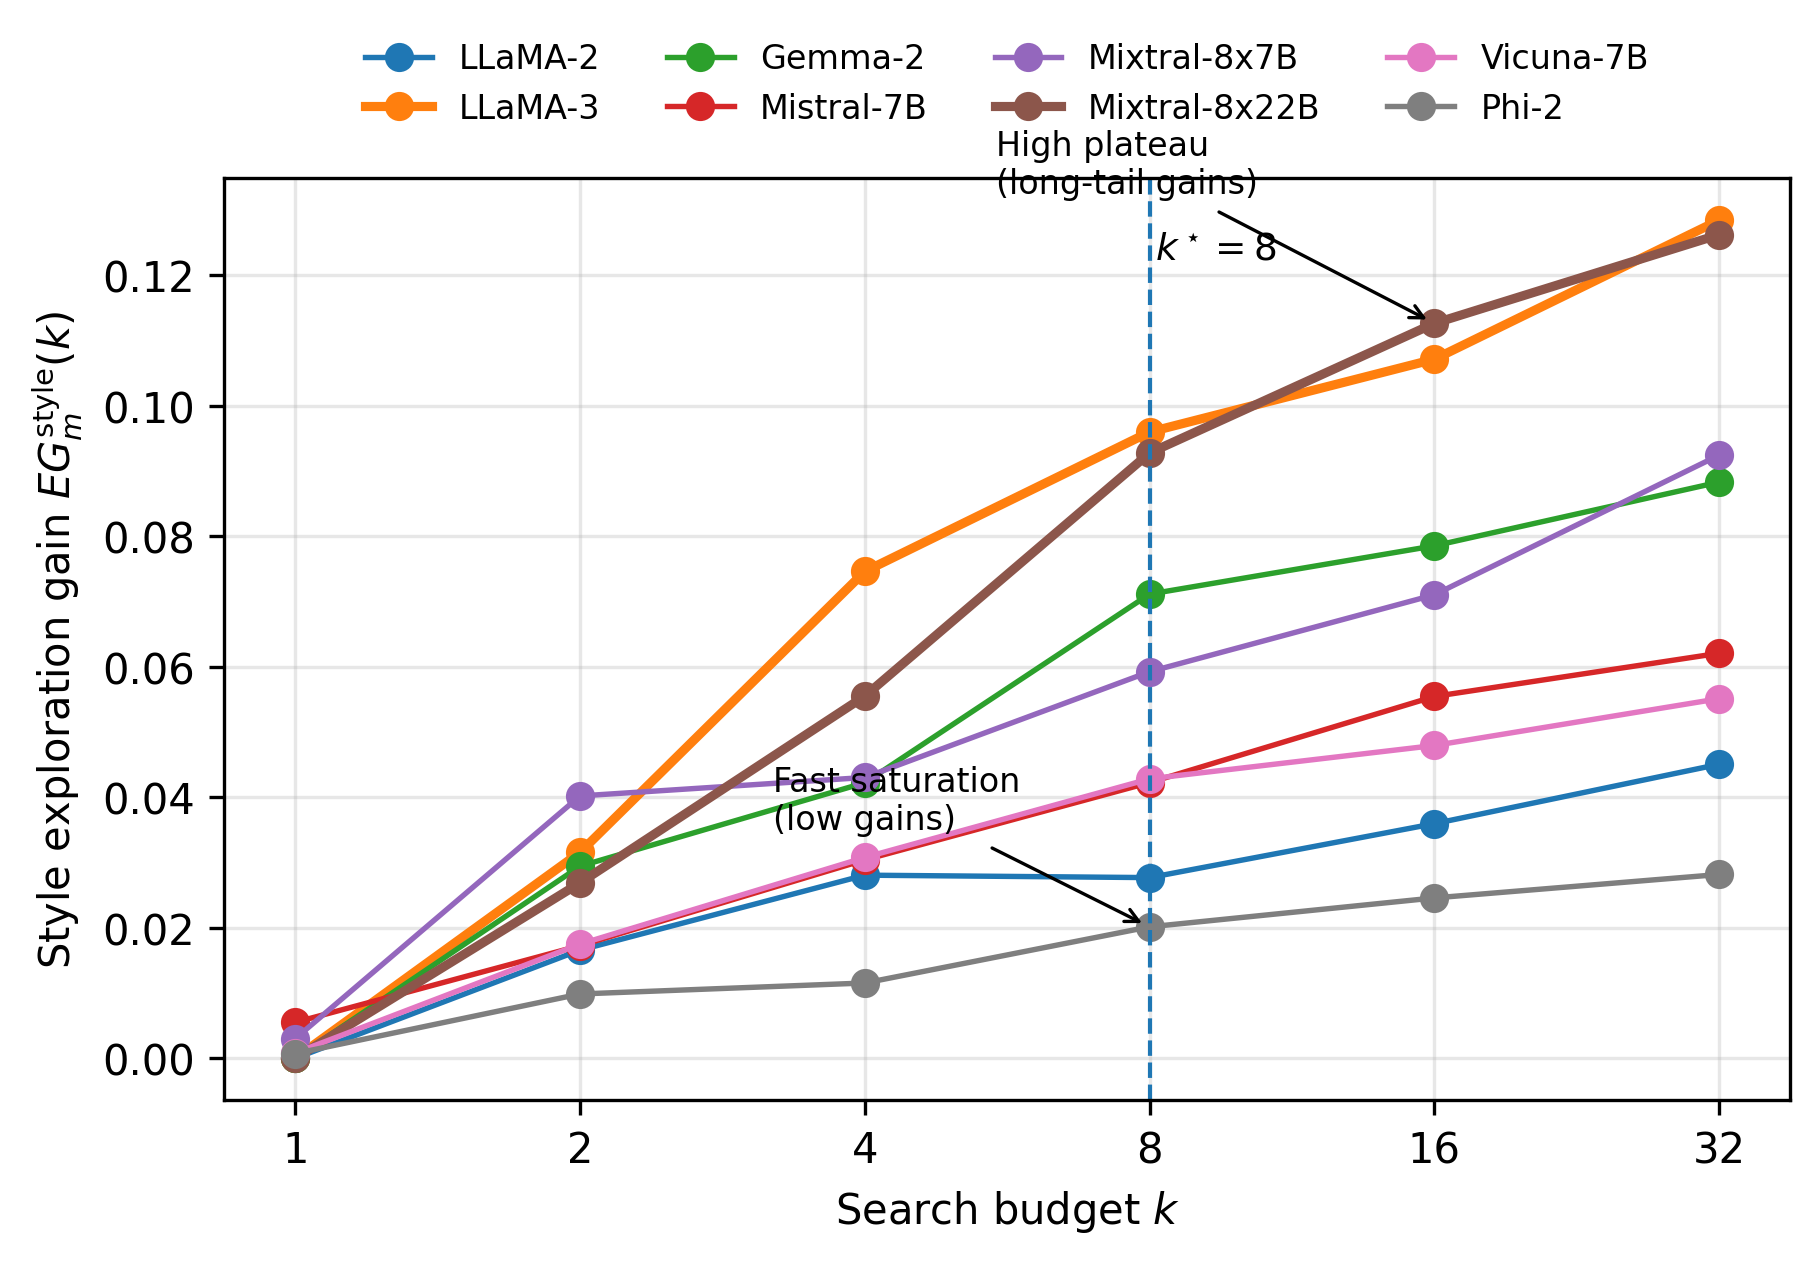
\includegraphics[width=\textwidth]{ICL/instrusum_eg_style_vs_k (1).png}
  \caption{\textbf{Style exploration gain as a function of search budget.}
  For each model $m$, we plot the \textbf{style exploration gain}
  $EG^{\text{style}}_m(k)$ on InstruSum as the search budget $k$ increases
  from 1 (greedy decoding) to 32 samples.
  Gains rise sharply between $k{=}2$ and $k{=}8$ and mostly \emph{saturate}
  by $k^\star{=}8$.
  Larger, recent models such as \textbf{LLaMA--3} and
  \textbf{Mixtral--8$\times$22B} reach higher plateaus
  ($EG^{\text{style}}_m(k^\star)\!\approx\!0.10$--$0.13$), whereas smaller
  models like \textbf{Phi--2} show \emph{fast saturation with low gains},
  indicating limited headroom for improving instruction adherence via search.
  Overall, the figure illustrates that \emph{distributional exploration}
  systematically improves style/constraint satisfaction, but the attainable
  gains are strongly \emph{model--dependent}.}
  \label{fig:instrusum_eg_style_vs_k}
\end{figure*}

% ================== Figure: EG^ICL_m vs EG^style_m(k*) =======================
\begin{figure*}[ht!]
  \centering
  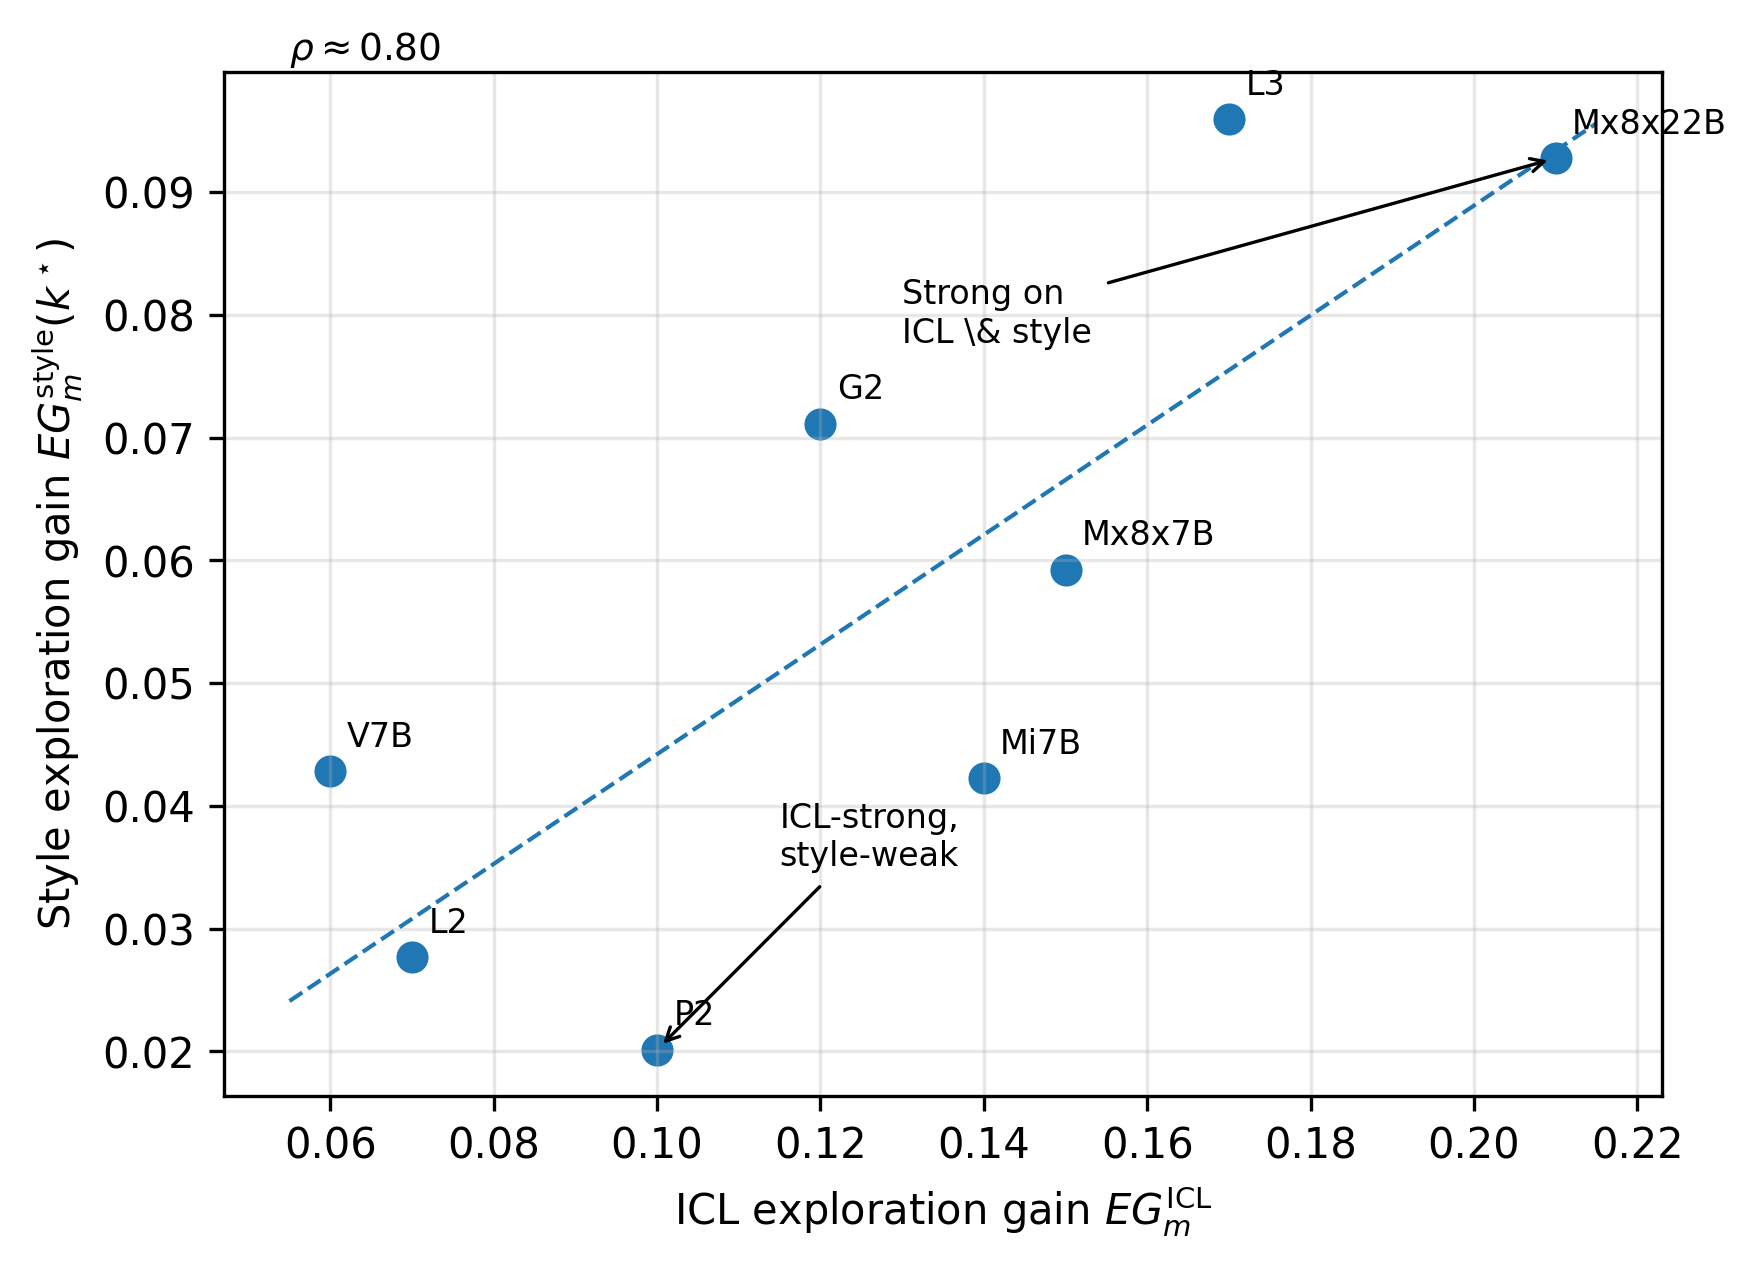
\includegraphics[width=\textwidth]{ICL/instrusum_eg_style_vs_icl_scatter (1).png}
  \caption{\textbf{Linking ICL exploration gains to style exploration gains.}
  Each point is a model $m$, with the x--axis showing its
  \textbf{ICL exploration gain} $EG^{\text{ICL}}_m$ on BESSTIE and the y--axis
  showing its \textbf{style exploration gain} $EG^{\text{style}}_m(k^\star)$
  on InstruSum at $k^\star{=}8$.
  The regression line and correlation ($\rho{\approx}0.80$) indicate that
  models with larger ICL gains typically also gain more in style/constraint
  satisfaction.
  Outliers such as \textbf{Phi--2} (\emph{ICL--strong, style--weak}) and
  \textbf{Mixtral--8$\times$22B} (\emph{strong on both}) show that this
  relationship is \emph{architecture--dependent}.
  Together with Figure~\ref{fig:instrusum_eg_style_vs_k}, this scatter plot
  supports our claim that \emph{distributional exploration} surfaces latent
  abilities in both ICL and style--constrained generation, while the degree to
  which they are buried under greedy decoding is highly \emph{model--specific}.}
  \label{fig:instrusum_eg_style_vs_icl_scatter}
\end{figure*}






















\subsubsection{How Much Exploration is Enough, and Where Do Gains Come From?}
\label{subsubsec:style-eg-analysis}

Figures~\ref{fig:instrusum_eg_style_vs_k}
and~\ref{fig:instrusum_eg_style_vs_icl_scatter}, together with
Table~\ref{tab:instrusum_breakdown}, summarize how \emph{distributional
exploration} translates into improved instruction following on
InstruSum, and how these gains relate back to the few--shot ICL gains
observed on BESSTIE.

\paragraph{Style exploration gain as a function of budget.}
Figure~\ref{fig:instrusum_eg_style_vs_k} plots, for each open model $m$,
the \textbf{style exploration gain} $EG^{\text{style}}_m(k)$ as the
search budget $k$ increases from $1$ (degenerate greedy decoding) up to
$32$ samples. Across models, the curves show a distinctive pattern:
\emph{\textbf{most of the benefit arrives quickly}}. Gains typically
rise sharply between $k{=}2$ and $k{=}8$ and then \emph{saturate} or
flatten by $k^\star{\approx}8$. Larger, recent backbones such as
\textbf{LLaMA--3} and \textbf{Mixtral--8$\times$22B} reach higher
plateaus (style exploration gains
$EG^{\text{style}}_m(k^\star)\!\approx\!0.10$--$0.13$), indicating that
they hide a substantial amount of instruction--compliant mass that only
multi--sample search uncovers. In contrast, smaller models such as
\textbf{Phi--2} show \emph{fast saturation with low gains}, suggesting
that there is simply less probability mass in their success sets $S_i$
to begin with. Operationally, the figure suggests a simple rule:
\emph{a small budget $k \in \{4,8\}$ is often enough to harvest the
majority of style/constraint gains}, with diminishing returns beyond
that point.

\paragraph{Linking style exploration to ICL exploration.}
Figure~\ref{fig:instrusum_eg_style_vs_icl_scatter} connects these
InstruSum results back to the BESSTIE ICL analysis. Each point
corresponds to a model $m$, with the x--axis showing its
\textbf{ICL exploration gain} $EG^{\text{ICL}}_m$ on BESSTIE and the
y--axis showing its \textbf{style exploration gain}
$EG^{\text{style}}_m(k^\star)$ at $k^\star{=}8$ on InstruSum. The
regression line and correlation ($\rho{\approx}0.80$) reveal a clear,
\emph{\textbf{positive relationship}}: \emph{models that benefit more
from exploration in few--shot ICL tend also to benefit more in
style/constraint satisfaction}. Architectures such as
\textbf{Mixtral--8$\times$22B} sit in the \emph{strong--strong} corner
(high ICL and high style gains), while others like \textbf{Phi--2} fall
into an \emph{ICL--strong, style--weak} regime. This pattern supports
our claim that ``\emph{explorability}''---the degree to which greedy
decoding leaves performance on the table---is a \emph{shared but
architecture--dependent} property: some models bury both reasoning and
instruction--following abilities under a single deterministic trajectory,
while others expose these abilities unevenly across tasks.

\paragraph{Where do the gains actually come from?}
Table~\ref{tab:instrusum_breakdown} decomposes the effect of
multi--sample search into its \emph{semantic} and
\emph{constraint--level} components. For each open model $m$ we report
mean semantic adequacy $\overline{s}_{\text{sem}}$, the four constraint
scores $\overline{c}_{\text{len}}, \overline{c}_{\text{inc}},
\overline{c}_{\text{avoid}}, \overline{c}_{\text{style}}$, and the full
success rate $P_{\text{succ}}^{\text{style}}$ under \emph{greedy}
decoding and \emph{multi--sample} decoding with $k{=}8$. A consistent
pattern emerges: \emph{\textbf{distributional exploration nudges almost
every dimension upward}}, but the largest relative gains come from
\textbf{length} and \textbf{style}, not raw content quality. Across
LLaMA--3, Gemma--2, and both Mixtral variants,
$\overline{c}_{\text{len}}$ and $\overline{c}_{\text{style}}$ typically
jump by $\approx 0.07$--$0.13$, while semantic adequacy
$\overline{s}_{\text{sem}}$ improves more modestly
($\approx 0.02$--$0.03$). Inclusion $\overline{c}_{\text{inc}}$ also
moves in the right direction, whereas \emph{avoidance} is already high
under greedy decoding and sees only small refinements. In other words,
multi--sample search does \emph{not} mainly ``fix hallucinations''; it
\emph{\textbf{rebalances the trade--off}} between content and formatting
constraints, finding trajectories that still say the right thing while
much better respecting the requested length and style.

\paragraph{Model--specific headroom.}
The rightmost column of Table~\ref{tab:instrusum_breakdown} translates
these per--dimension shifts into \emph{full} instruction--following
success. Strong, recent models such as LLaMA--3, Gemma--2, and especially
Mixtral--8$\times$22B see \textbf{large absolute jumps} in
$P_{\text{succ}}^{\text{style}}$ under $k{=}8$ search
(e.g., from $0.48 \rightarrow 0.64$ for LLaMA--3 and
$0.49 \rightarrow 0.68$ for Mixtral--8$\times$22B), confirming that a
substantial fraction of instruction--compliant trajectories was present
but never reached by greedy decoding. Mid--tier models such as
Mistral--7B and Mixtral--8$\times$7B exhibit similar, slightly smaller
gains, while older or smaller backbones like Vicuna--7B and
\textbf{Phi--2} show \emph{only modest improvements}
(e.g., $0.30 \rightarrow 0.35$ for Phi--2), reflecting genuinely limited
mass in their success sets $S_i$.

Taken together with
Figures~\ref{fig:instrusum_eg_style_vs_k}
and~\ref{fig:instrusum_eg_style_vs_icl_scatter}, the breakdown in
Table~\ref{tab:instrusum_breakdown} reinforces our central message:
\emph{\textbf{what greedy decoding hides is not just more ``good
summaries'', but better points on the multi--objective frontier}}, where
semantic adequacy and all four constraint axes are jointly satisfied.
In this sense, the InstruSum results mirror our findings on BESSTIE:
\emph{stochastic, multi--sample decoding reveals instruction--following
competence that is already encoded in $p_\theta(\tau \mid d_i, r_i)$ but
systematically suppressed by strictly deterministic inference.}












\subsubsection{Semantic--Constraint Density Landscapes on InstruSum}
\label{subsec:semcon-landscapes}

Figures~\ref{fig:instrusum_semantic_constraint_llama2}--%
\ref{fig:instrusum_semantic_constraint_phi2}
(aggregated in
Figure~\ref{fig:instrusum_semantic_constraint_all_models})
show, for each model $m$, \emph{where its probability mass actually
lives} in the \textbf{semantic--constraint space} defined in
\S\ref{subsec:style-metrics}.  For every InstruSum instance $i$ and model
$m$, we draw a pool of stochastic candidates
$\{\tau_i^{(j)}\}_{j=1}^K$ using the same base sampler as in our
multi--sample experiments (temperature $T{=}0.7$, nucleus $p{=}0.9$).
For each trajectory we compute the semantic adequacy score
$s_{\text{sem}}(\tau_i^{(j)}; d_i, y_i^\star)$ and the
\emph{joint constraint score}
$c_{\text{joint}}(\tau_i^{(j)}) = c_{\text{len}} \cdot c_{\text{inc}}
\cdot c_{\text{avoid}} \cdot c_{\text{style}}$
(\S\ref{subsec:style-metrics}).  We then aggregate all
$\bigl(s_{\text{sem}}, c_{\text{joint}}\bigr)$ pairs for model $m$,
estimate a smoothed 2D density on $[0,1]^2$, and plot it as a
\textbf{3D surface}.  The horizontal axes are \emph{semantic adequacy}
and \emph{joint constraint satisfaction}; the vertical axis depicts how
much probability mass the model places in each region under its
instruction--conditioned distribution $p_\theta(\cdot \mid d_i,r_i)$.

Across panels~\ref{fig:instrusum_semantic_constraint_llama2}--%
\ref{fig:instrusum_semantic_constraint_phi2}, a strikingly consistent
picture emerges.  Many instruction--tuned LLMs exhibit a tall, narrow
\emph{\textbf{under--constrained ridge}}: a band where
$s_{\text{sem}}(\tau)$ is reasonably high (the summary mostly captures
the article) but $c_{\text{joint}}(\tau)$ is low to moderate, meaning
that length, inclusion, avoidance, and style requirements are only
partially satisfied.  This ridge dominates the landscapes for models
such as \textbf{LLaMA--2}, \textbf{Vicuna--7B}, and \textbf{Phi--2}
(Figures~\ref{fig:instrusum_semantic_constraint_llama2},
\ref{fig:instrusum_semantic_constraint_vicuna7b}, and
\ref{fig:instrusum_semantic_constraint_phi2}), with only a thin,
low--density tail reaching into the
\emph{\textbf{high semantics \& high constraints}} corner.  In these
cases, deterministic greedy decoding is effectively \emph{anchored to
the ridge}: it reliably produces summaries that ``get the gist'' but
ignore parts of the requested format or style, even though well--aligned
candidates \emph{do} exist in the tails of the distribution.

Newer and larger backbones---most notably \textbf{LLaMA--3},
\textbf{Gemma--2}, and the mixture--of--experts models
\textbf{Mixtral--8$\times$7B} and \textbf{Mixtral--8$\times$22B}
(Figures~\ref{fig:instrusum_semantic_constraint_llama3}--%
\ref{fig:instrusum_semantic_constraint_mixtral8x22b})---show the same
ridge but with a pronounced \emph{shift of mass} toward the upper--right
corner of Figure~\ref{fig:instrusum_semantic_constraint_all_models}.
For these models, the peak density lies around
$s_{\text{sem}}(\tau) \in [0.65,0.85]$ and
$c_{\text{joint}}(\tau) \in [0.35,0.60]$, indicating that they
\emph{naturally place substantial probability} on summaries that jointly
respect content and stylistic constraints.  Here, the under--constrained
ridge becomes secondary: a nontrivial portion of the distribution is
already near the semantic--constraint Pareto frontier, so even modest
multi--sample search can routinely surface well--aligned summaries.
By contrast, \textbf{Phi--2}
(Figure~\ref{fig:instrusum_semantic_constraint_phi2}) concentrates mass
in a steep, low--constraint ridge with only a tiny high--constraint
island, explaining why its style exploration gains plateau quickly and
at low absolute levels in Figure~\ref{fig:instrusum_eg_style_vs_k}.

These density landscapes provide a geometric explanation for the
quantitative results in
Figures~\ref{fig:instrusum_eg_style_vs_k}--%
\ref{fig:instrusum_eg_style_vs_icl_scatter} and the per--dimension
breakdown in Table~\ref{tab:instrusum_breakdown}.  When the
high semantics \& high constraints region carries \emph{substantial
mass} (e.g., LLaMA--3, Mixtral--8$\times$22B), multi--sample decoding
with a small budget $k$ can move outputs from the under--constrained
ridge into this upper--right plateau, yielding large positive
$EG^{\text{style}}_m(k)$ and noticeable gains in all constraint
dimensions.  When that region is a thin, low--density island (e.g.,
Vicuna--7B, Phi--2), additional sampling helps much less: even a
distributionally aware search policy rarely stumbles into genuinely
well--aligned trajectories.  The central takeaway is thus
\emph{\textbf{geometric}}: many apparent failures to follow detailed
style and format instructions are not hard limits of
$p_\theta(\cdot \mid d_i,r_i)$, but symptoms of a decoding policy that
is stuck on an under--constrained ridge and never explores the
high--quality corner of the semantic--constraint landscape.





% ===================== Figure 1: Panels (a)--(d) =====================
\begin{figure*}[ht!]
  \centering

  % (a) LLaMA-2
  \begin{subfigure}[t]{0.48\textwidth}
    \centering
    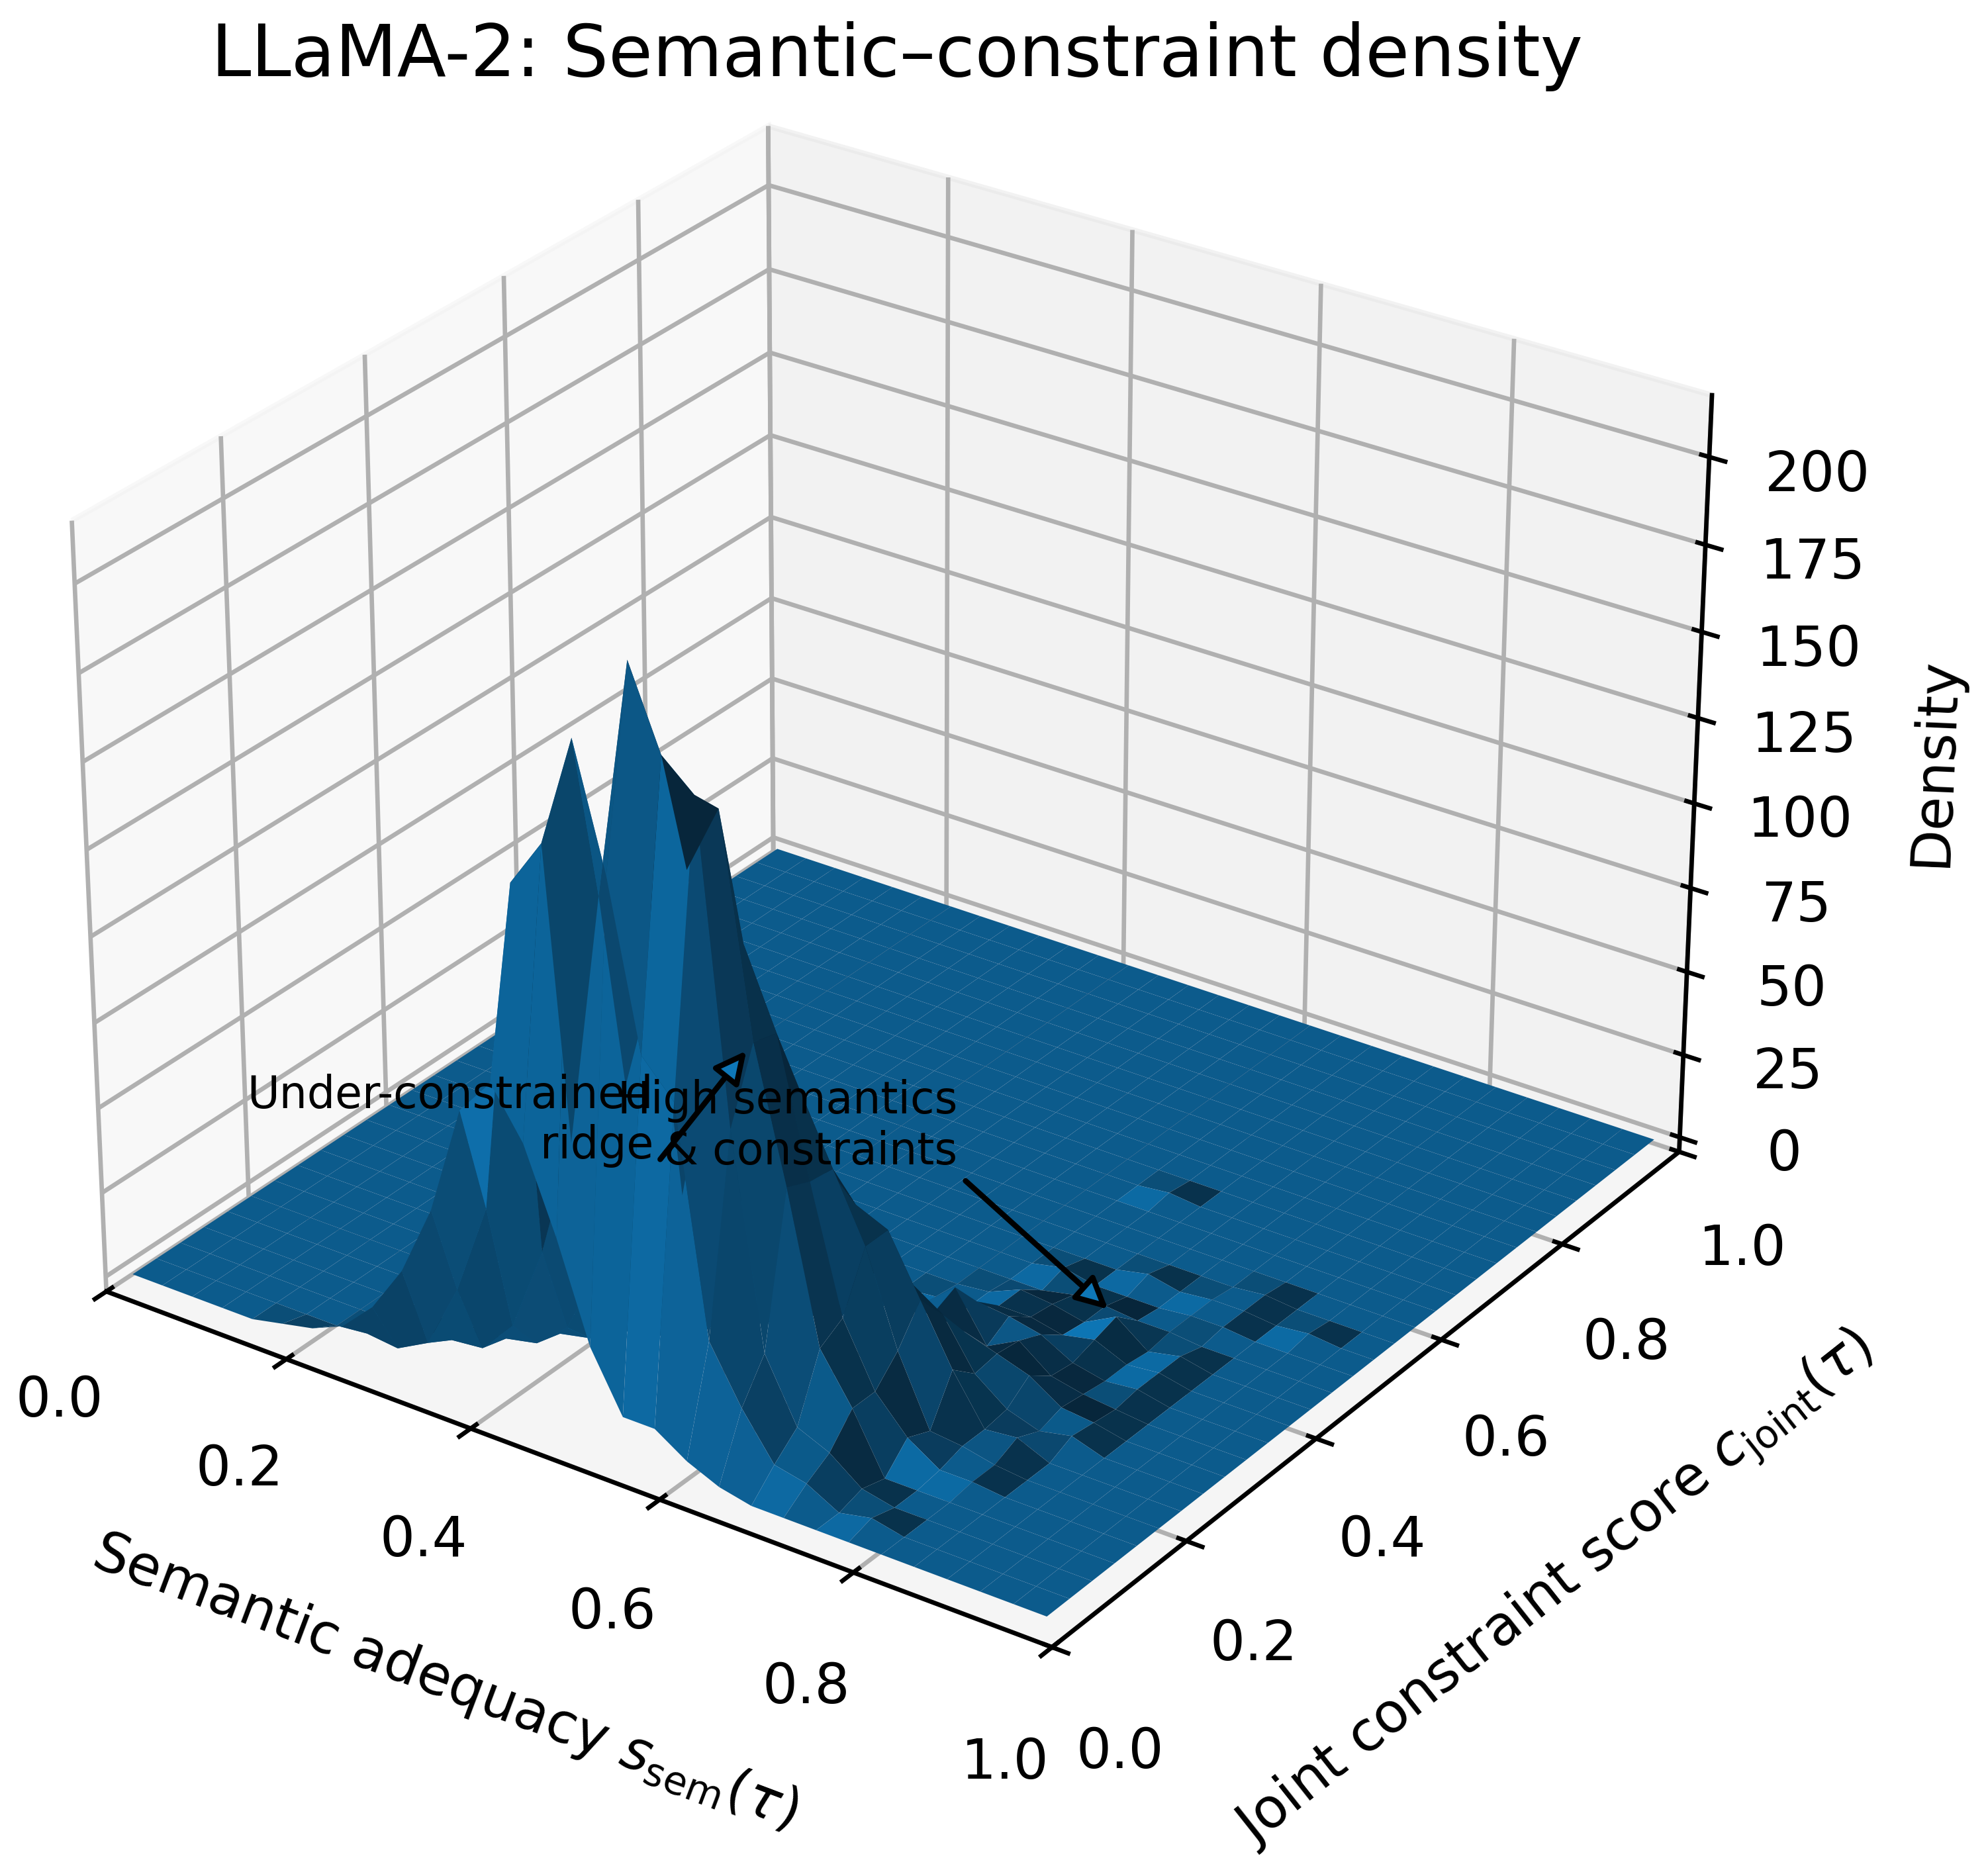
\includegraphics[width=\linewidth]{ICL/instrusum_pareto_surface_llama2_annotated.png}
    \subcaption{\textbf{LLaMA--2.} 
    The joint density over \emph{semantic adequacy} $s_{\mathrm{sem}}(\tau)$ and
    \emph{joint constraint score} $c_{\mathrm{joint}}(\tau)$ reveals a tall,
    narrow \textbf{under--constrained ridge}: most candidates concentrate in
    $s_{\mathrm{sem}}(\tau) \in [0.50, 0.70]$ but only
    $c_{\mathrm{joint}}(\tau) \in [0.15, 0.35]$,
    meaning that LLaMA--2 frequently captures the gist of the article while ignoring length, inclusion, and style requirements.
    The arrowed point near
    $(s_{\mathrm{sem}}, c_{\mathrm{joint}}) \approx (0.70, 0.45)$ highlights a
    \emph{thin but nontrivial} region where well--balanced, constraint--respecting
    summaries exist but are rarely selected by greedy decoding.}
    \label{fig:instrusum_semantic_constraint_llama2}
  \end{subfigure}\hfill
  %
  % (b) LLaMA-3
  \begin{subfigure}[t]{0.48\textwidth}
    \centering
    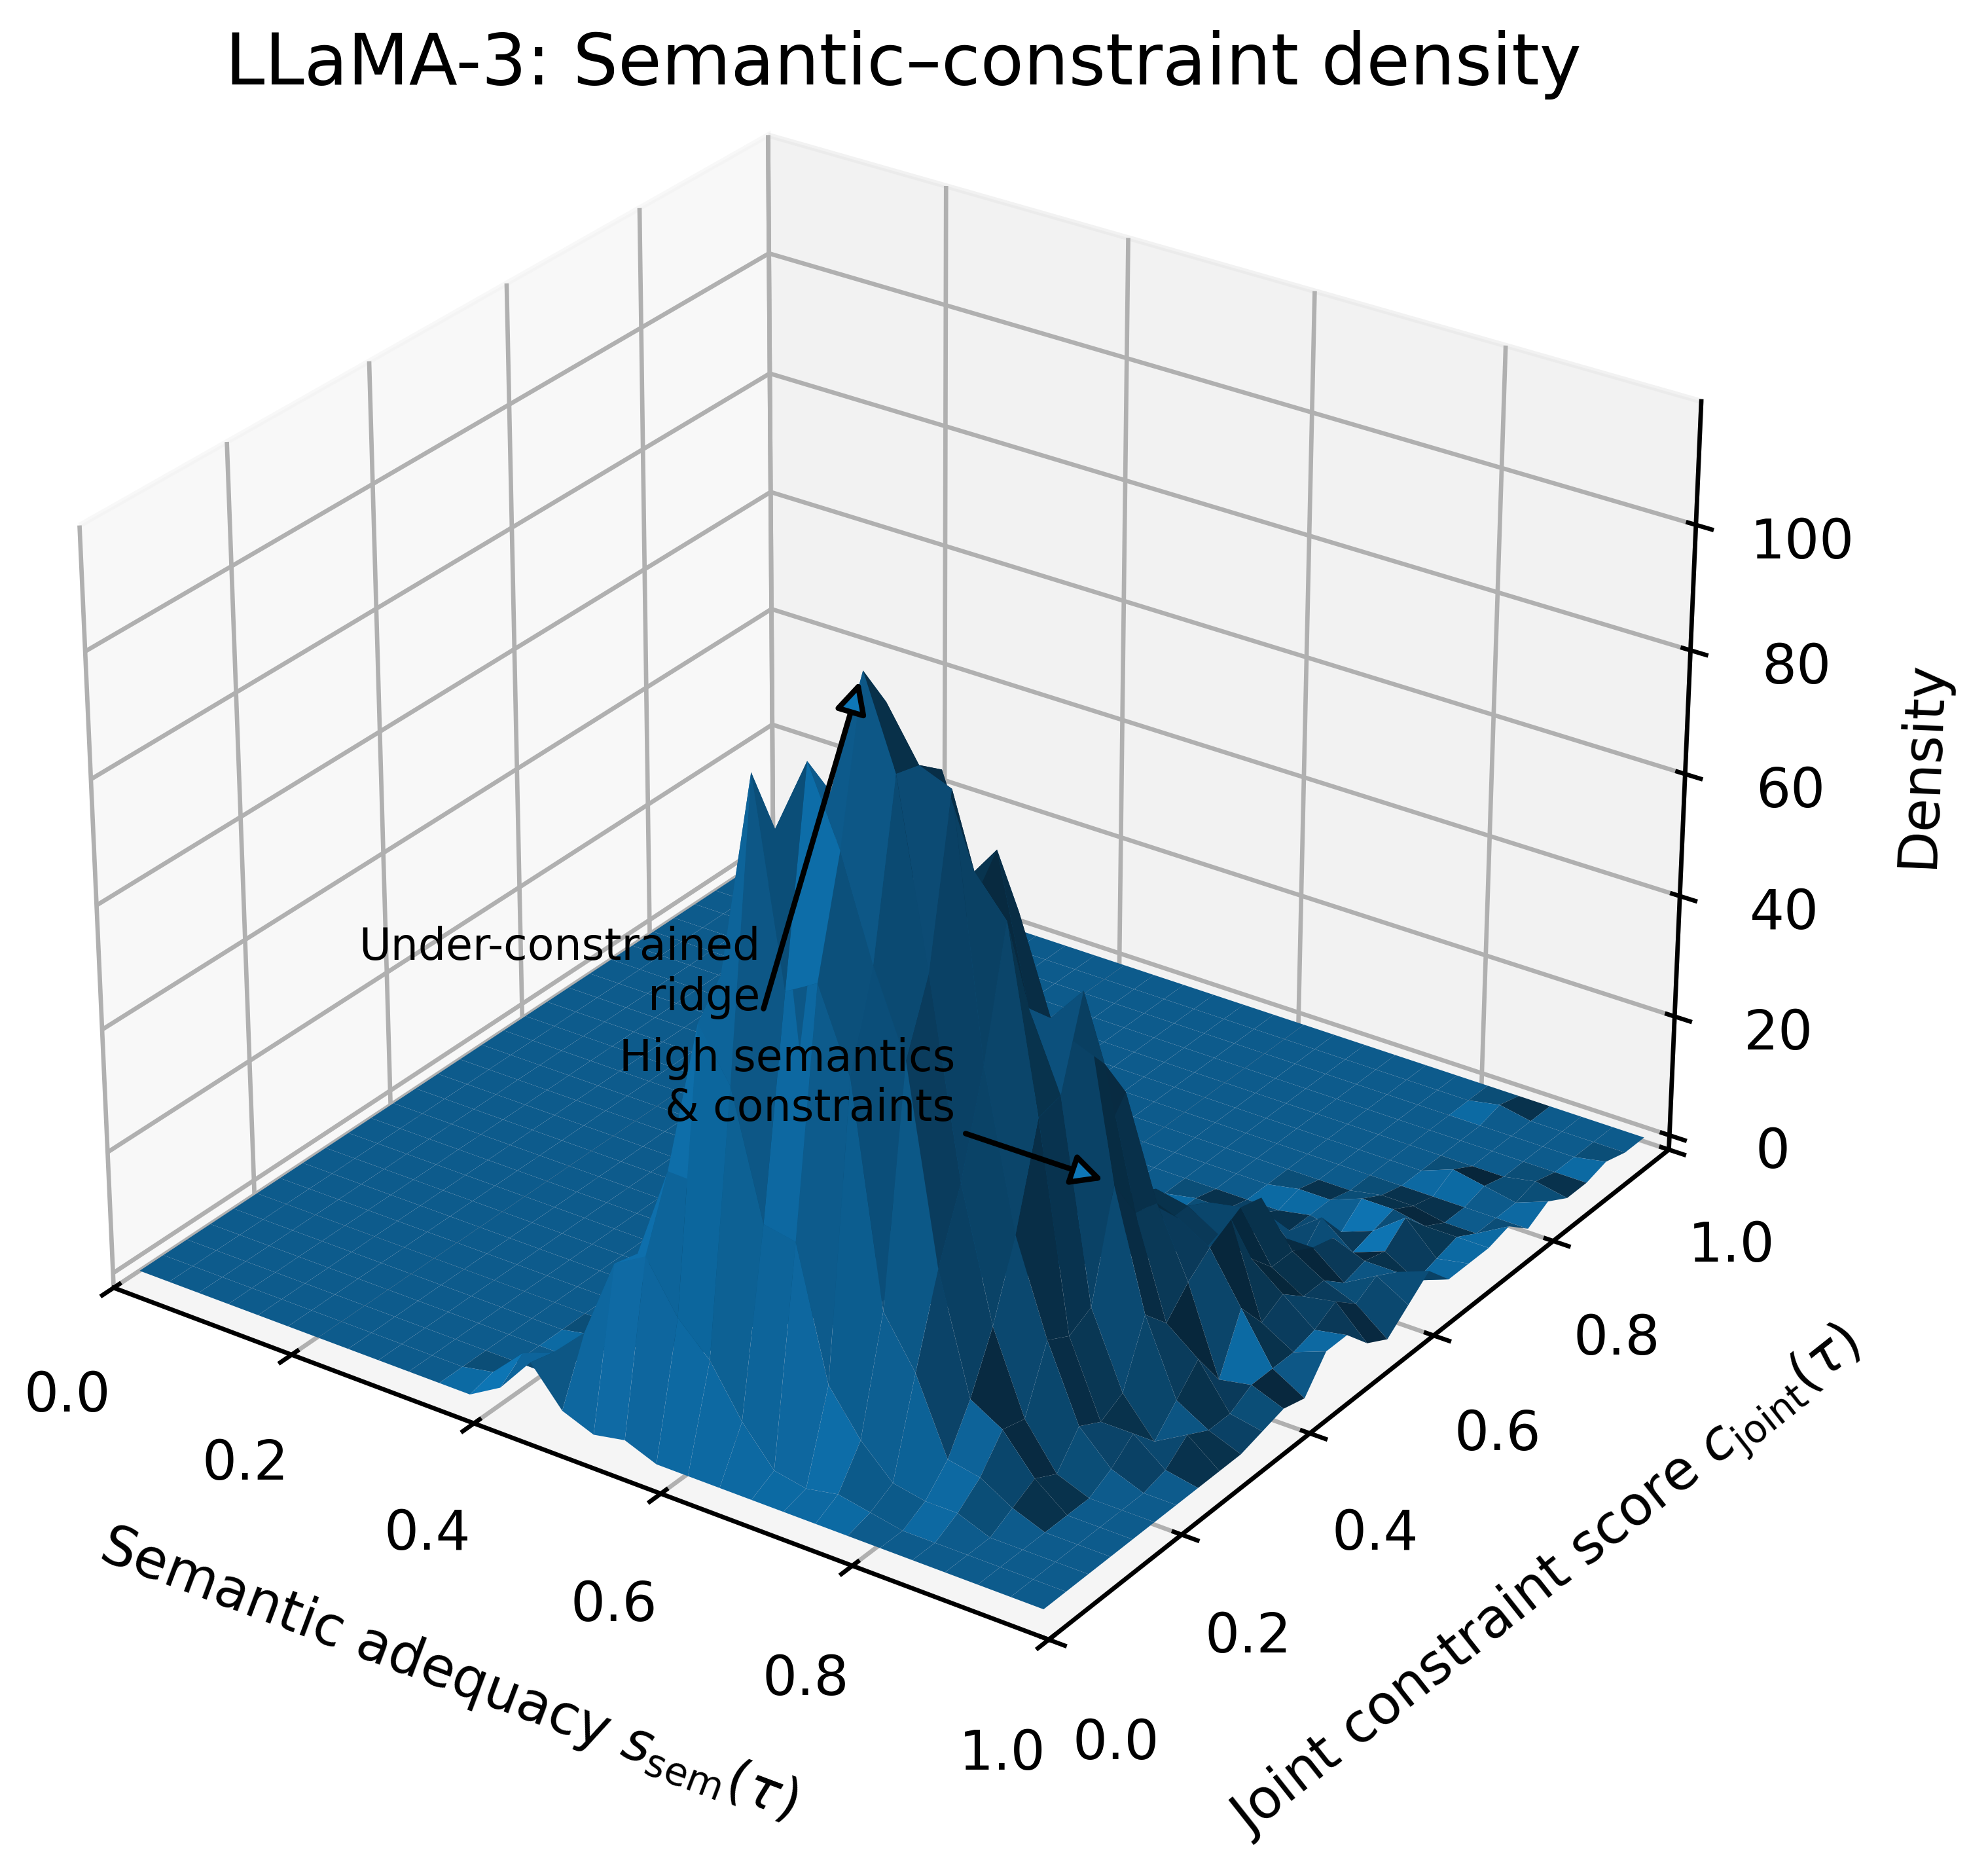
\includegraphics[width=\linewidth]{ICL/instrusum_pareto_surface_llama3_annotated.png}
    \subcaption{\textbf{LLaMA--3.}
    For the newer LLaMA--3 model, the density mass shifts noticeably toward the
    \textbf{upper--right} of the plane:
    the bulk of candidates lies in $s_{\mathrm{sem}}(\tau) \in [0.60, 0.80]$
    and $c_{\mathrm{joint}}(\tau) \in [0.25, 0.50]$.
    The under--constrained ridge is still visible at
    $c_{\mathrm{joint}}(\tau) \lesssim 0.30$, but the arrowed
    \emph{high semantics \& constraints} region around
    $(0.70\!-\!0.80, 0.45\!-\!0.60)$ now carries substantial density,
    indicating that LLaMA--3 often places mass directly on approximately
    Pareto--optimal summaries that satisfy both content and stylistic hints.}
    \label{fig:instrusum_semantic_constraint_llama3}
  \end{subfigure}

  %\vspace{0.7em}

  % (c) Gemma-2
  \begin{subfigure}[t]{0.48\textwidth}
    \centering
    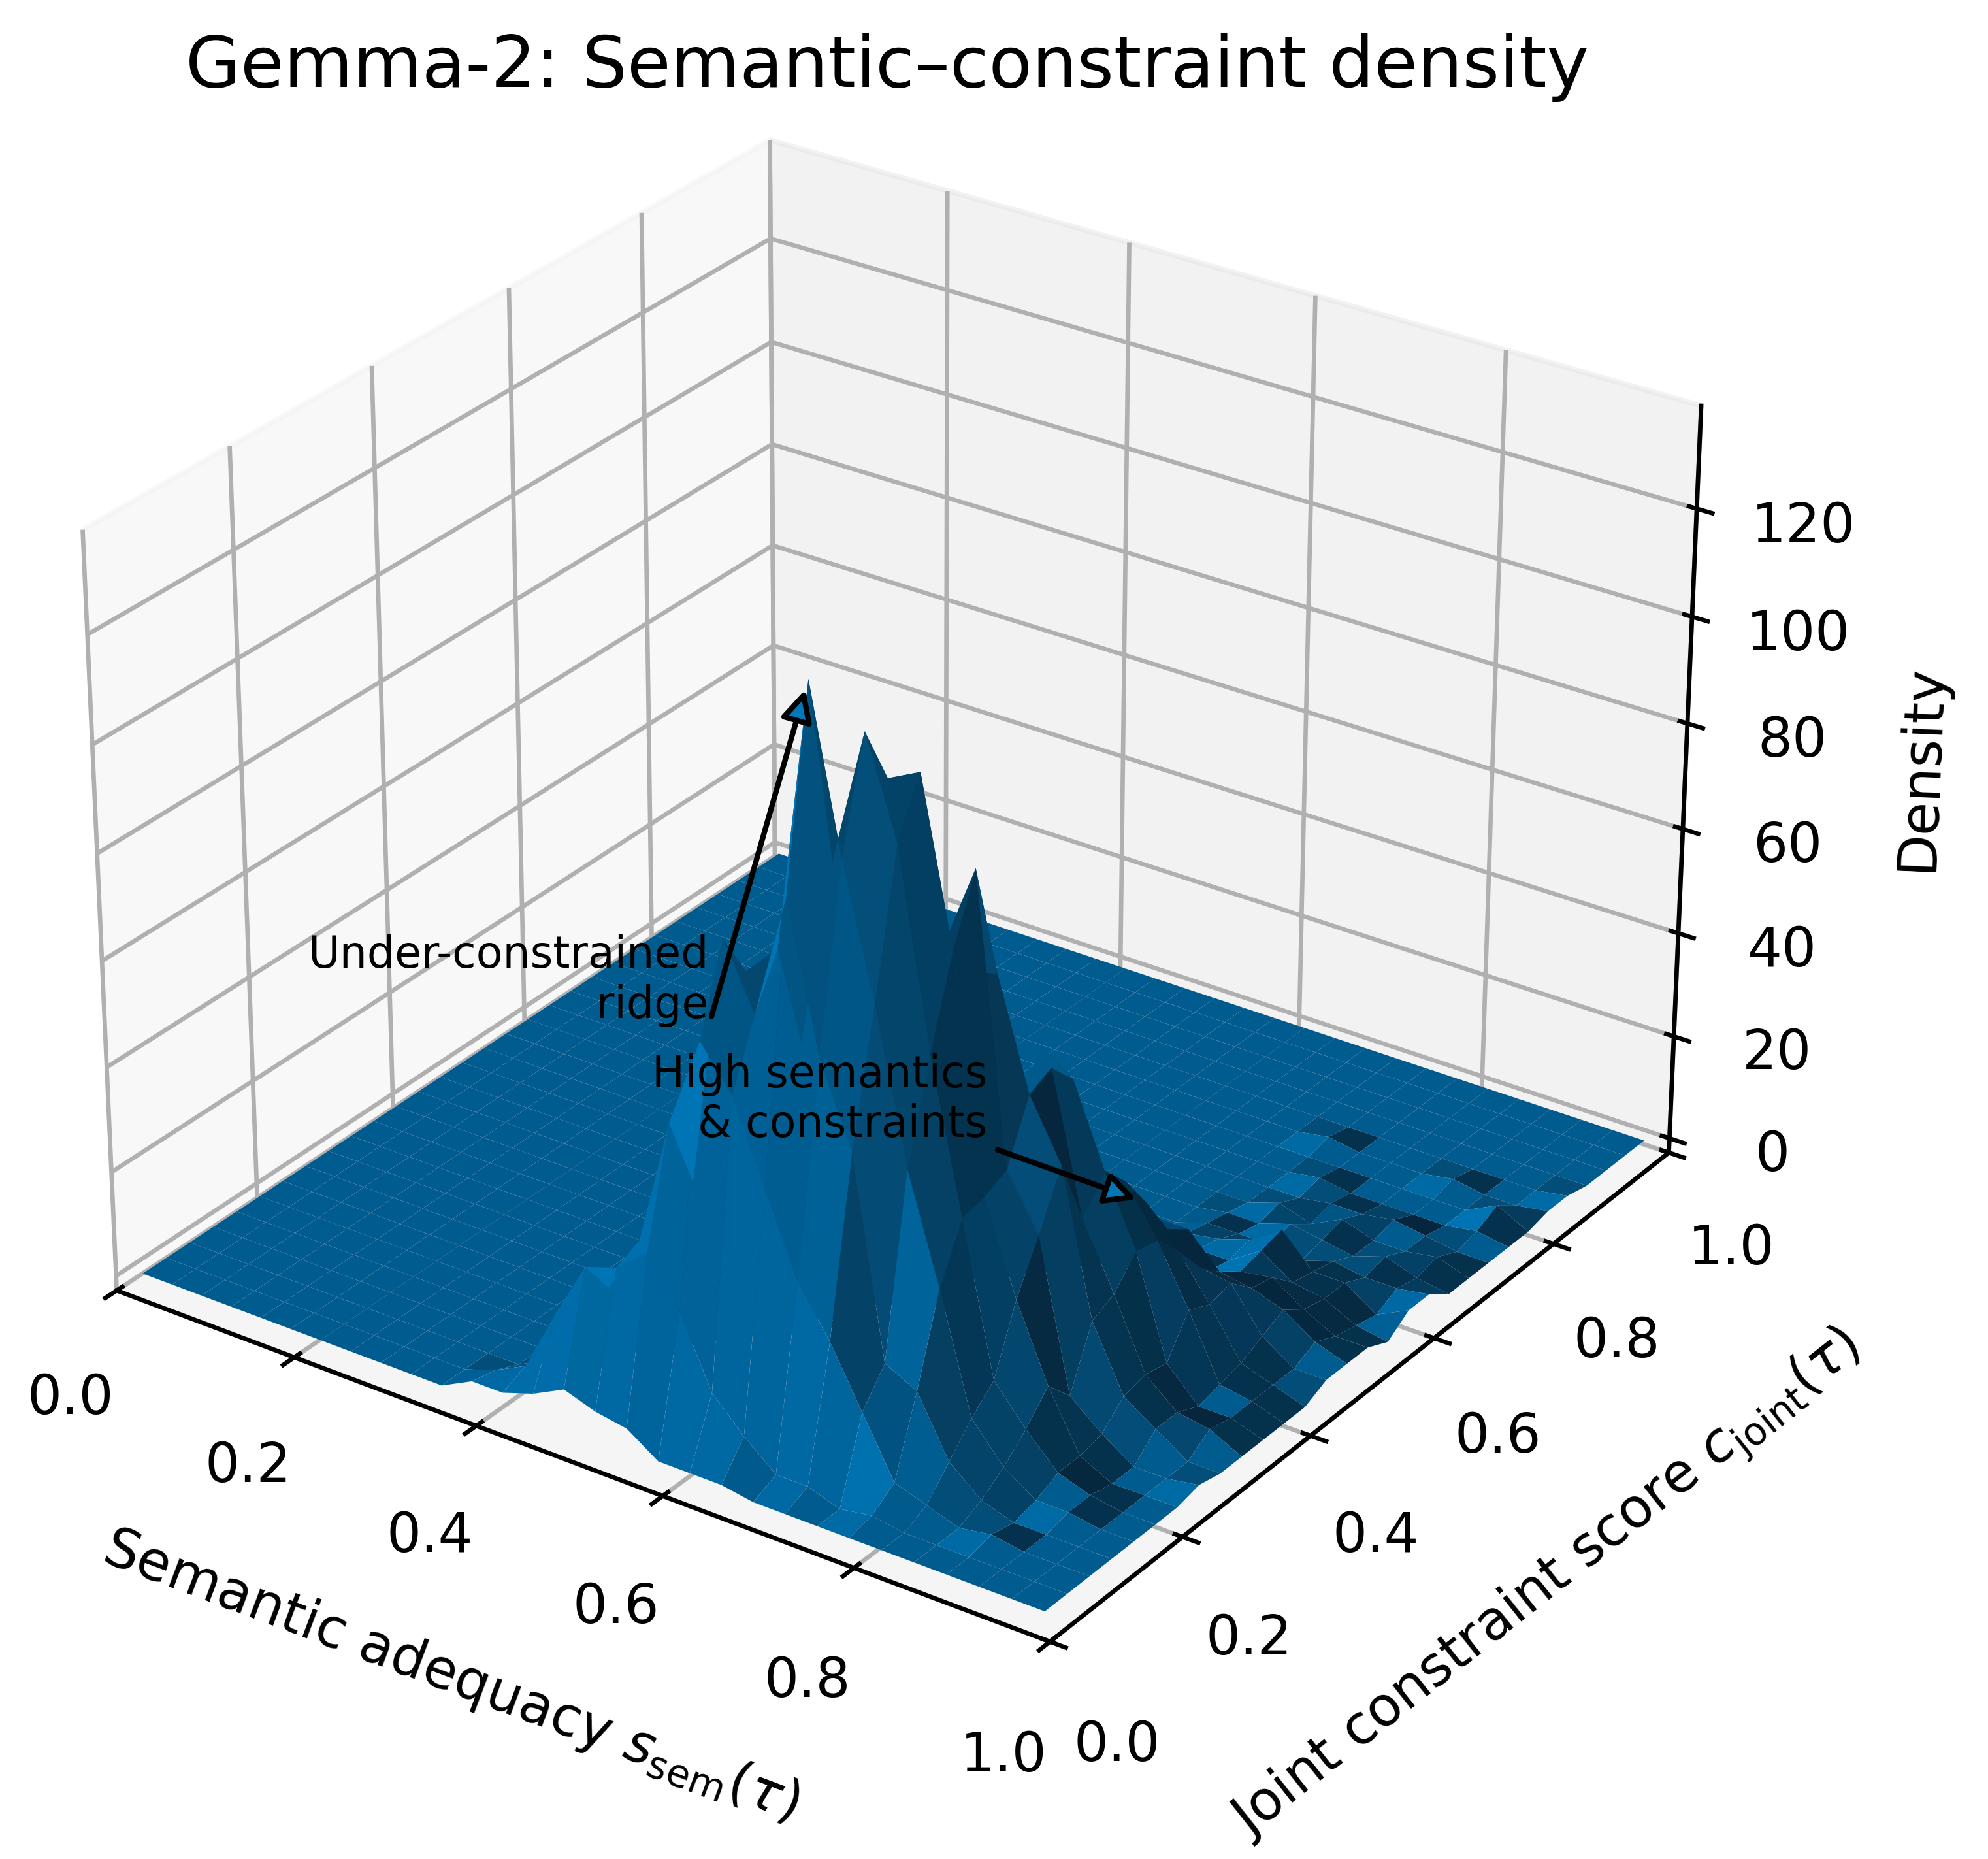
\includegraphics[width=\linewidth]{ICL/instrusum_pareto_surface_gemma2_annotated.png}
    \subcaption{\textbf{Gemma--2.}
    Gemma--2 shows a \emph{broader} and more \textbf{spread--out} landscape:
    candidates typically occupy $s_{\mathrm{sem}}(\tau) \in [0.55, 0.75]$ and
    $c_{\mathrm{joint}}(\tau) \in [0.25, 0.55]$, with a visible secondary peak
    near $(0.70, 0.50)$.
    The under--constrained ridge at
    $c_{\mathrm{joint}}(\tau) \lesssim 0.30$ is less dominant than in
    LLaMA--2, suggesting that Gemma--2 is more willing to trade a small amount
    of semantic score to better respect formatting and style. 
    In other words, Gemma--2’s stochastic support contains a richer mix of
    \emph{semantics--heavy} and \emph{constraint--faithful} summaries.}
    \label{fig:instrusum_semantic_constraint_gemma2}
  \end{subfigure}\hfill
  %
  % (d) Mistral-7B
  \begin{subfigure}[t]{0.48\textwidth}
    \centering
    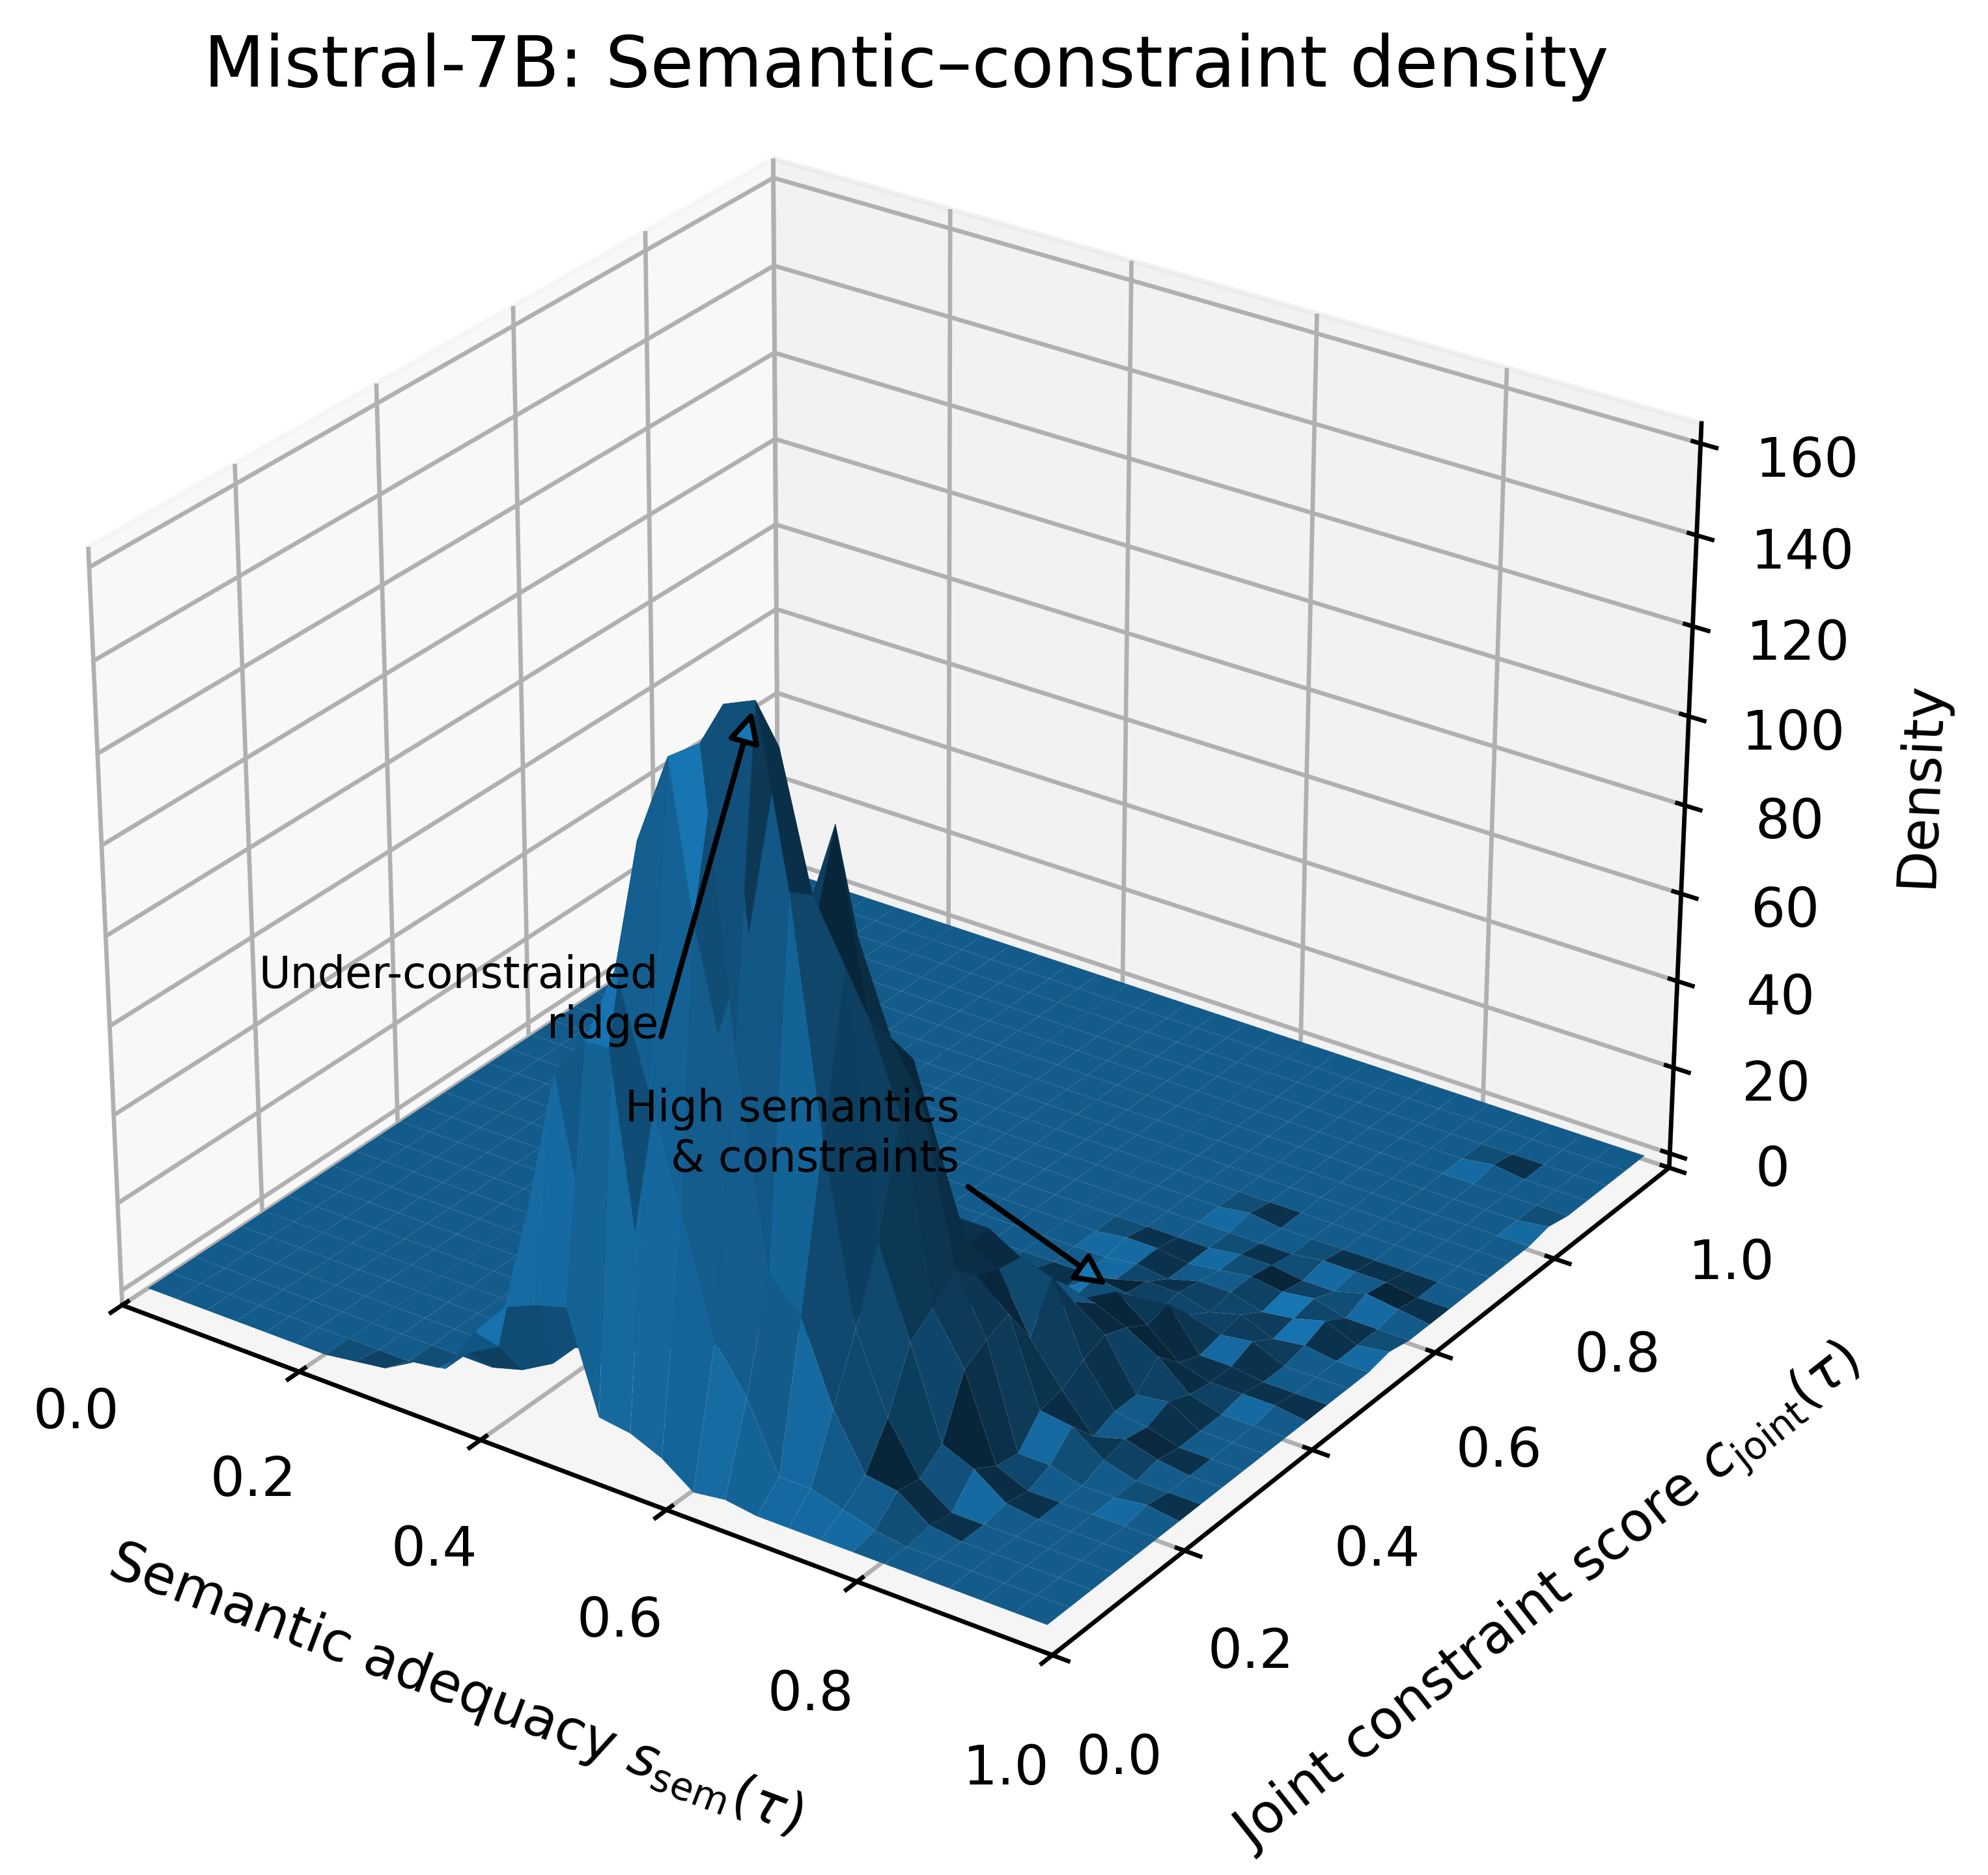
\includegraphics[width=\linewidth]{ICL/instrusum_pareto_surface_mistral7b_annotated.png}
    \subcaption{\textbf{Mistral--7B.}
    Mistral--7B exhibits a tall peak concentrated in
    $s_{\mathrm{sem}}(\tau) \in [0.55, 0.75]$ but with
    $c_{\mathrm{joint}}(\tau)$ mostly confined to $[0.15, 0.30]$,
    indicating that the model strongly prioritizes semantic coverage of the
    article over strict adherence to instruction constraints.
    The annotated under--constrained ridge therefore dominates the surface,
    while only a relatively \emph{thin and low--density} band of candidates
    reaches $c_{\mathrm{joint}}(\tau) \gtrsim 0.40$.
    This pattern makes Mistral--7B look stylistically weak under greedy
    decoding, even though the geometry reveals that higher--constraint
    summaries do exist in its sampling distribution.}
    \label{fig:instrusum_semantic_constraint_mistral7b}
  \end{subfigure}

  % no numbered global caption here
  \caption*{\textbf{Semantic--constraint density landscapes, part I.}
  Panels \textbf{(a)}--\textbf{(d)} show four representative models, illustrating
  how probability mass can be concentrated on an \emph{under--constrained ridge}
  even when higher--quality, constraint--respecting summaries are present in
  the tails of the distribution.}
\end{figure*}


% ===================== Figure 2: Panels (e)--(h) =====================
\begin{figure*}[ht!]
  \centering
  % make subfigure captions smaller
  \captionsetup[subfigure]{font=footnotesize}
  % continue subfigure lettering from (e)
  \setcounter{subfigure}{4}

  % (e) Mixtral-8x7B
  \begin{subfigure}[t]{0.46\textwidth}
    \centering
    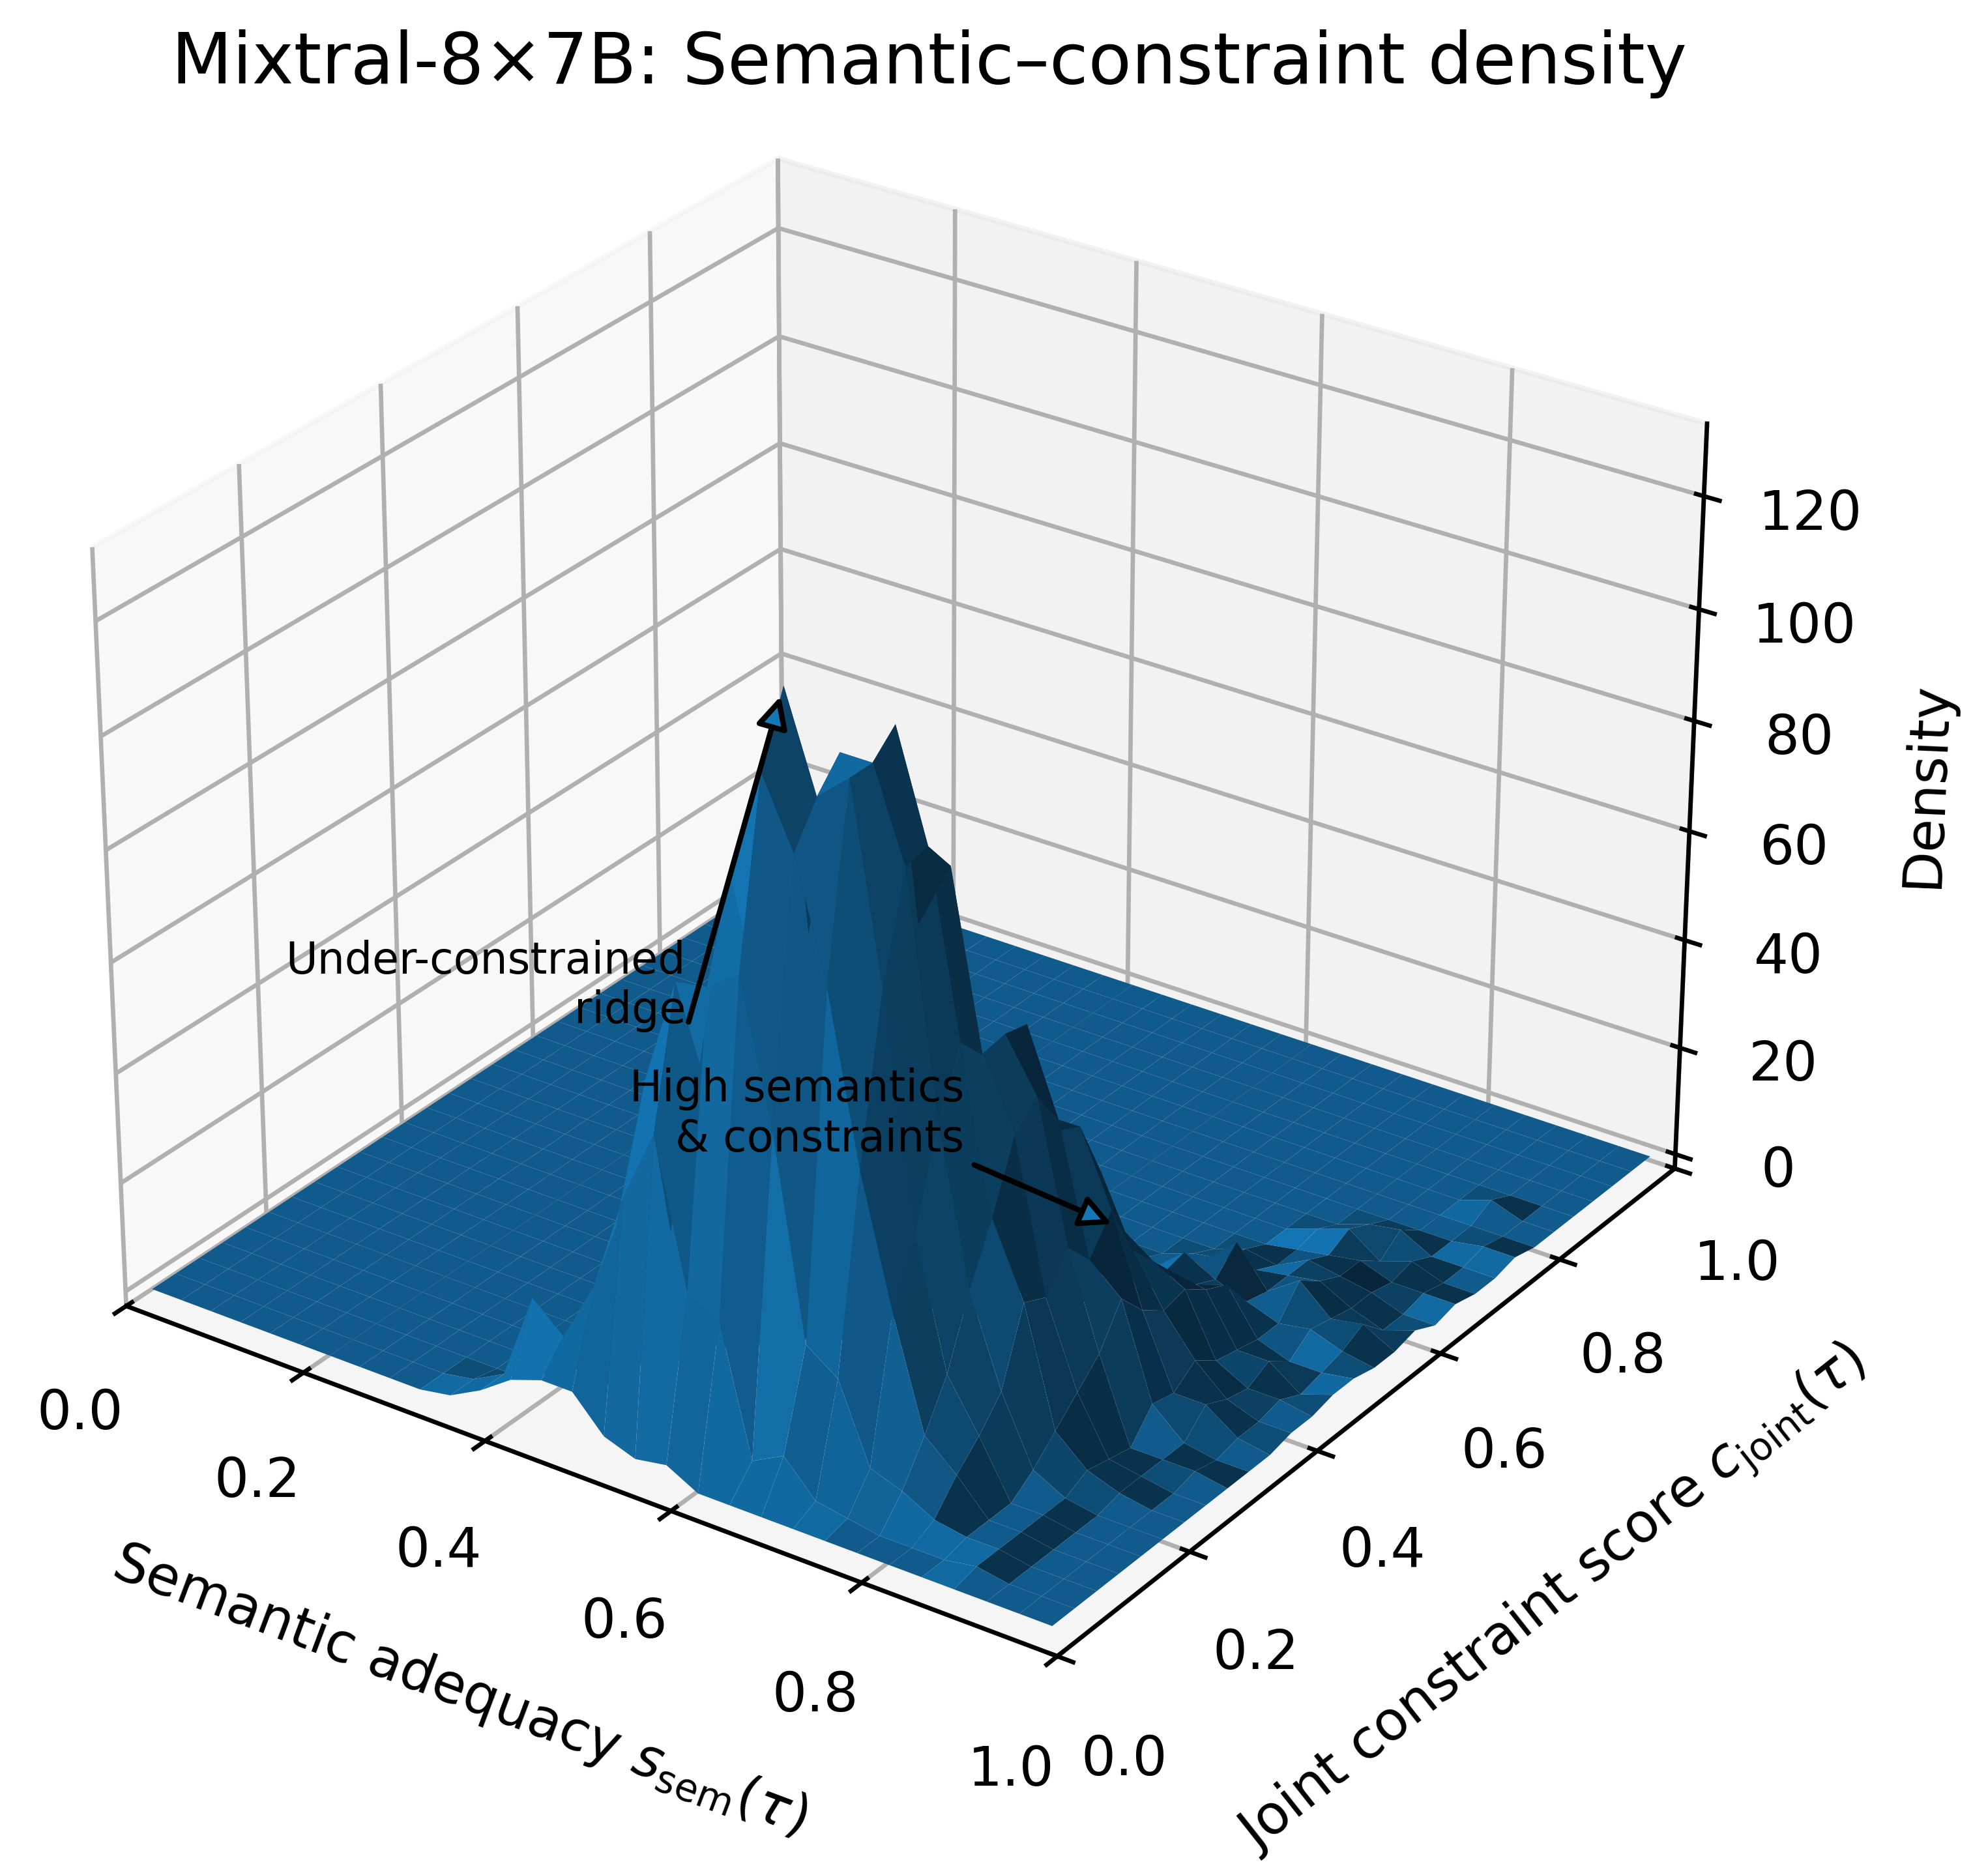
\includegraphics[width=\linewidth]{ICL/instrusum_pareto_surface_mixtral8x7b_annotated.png}
    \subcaption{\textbf{Mixtral--8$\times$7B.}
    The semantic--constraint landscape is \textbf{balanced}:
    most mass lies in $s_{\mathrm{sem}}(\tau) \in [0.60, 0.80]$ and
    $c_{\mathrm{joint}}(\tau) \in [0.30, 0.55]$.
    An under--constrained ridge remains at
    $c_{\mathrm{joint}}(\tau) \lesssim 0.30$, but the annotated peak in the
    upper--right shows many candidates that jointly achieve
    \emph{high semantics and strong constraint satisfaction}, so
    multi--sample decoding can routinely surface well aligned summaries.}
    \label{fig:instrusum_semantic_constraint_mixtral8x7b}
  \end{subfigure}\hfill
  %
  % (f) Mixtral-8x22B
  \begin{subfigure}[t]{0.46\textwidth}
    \centering
    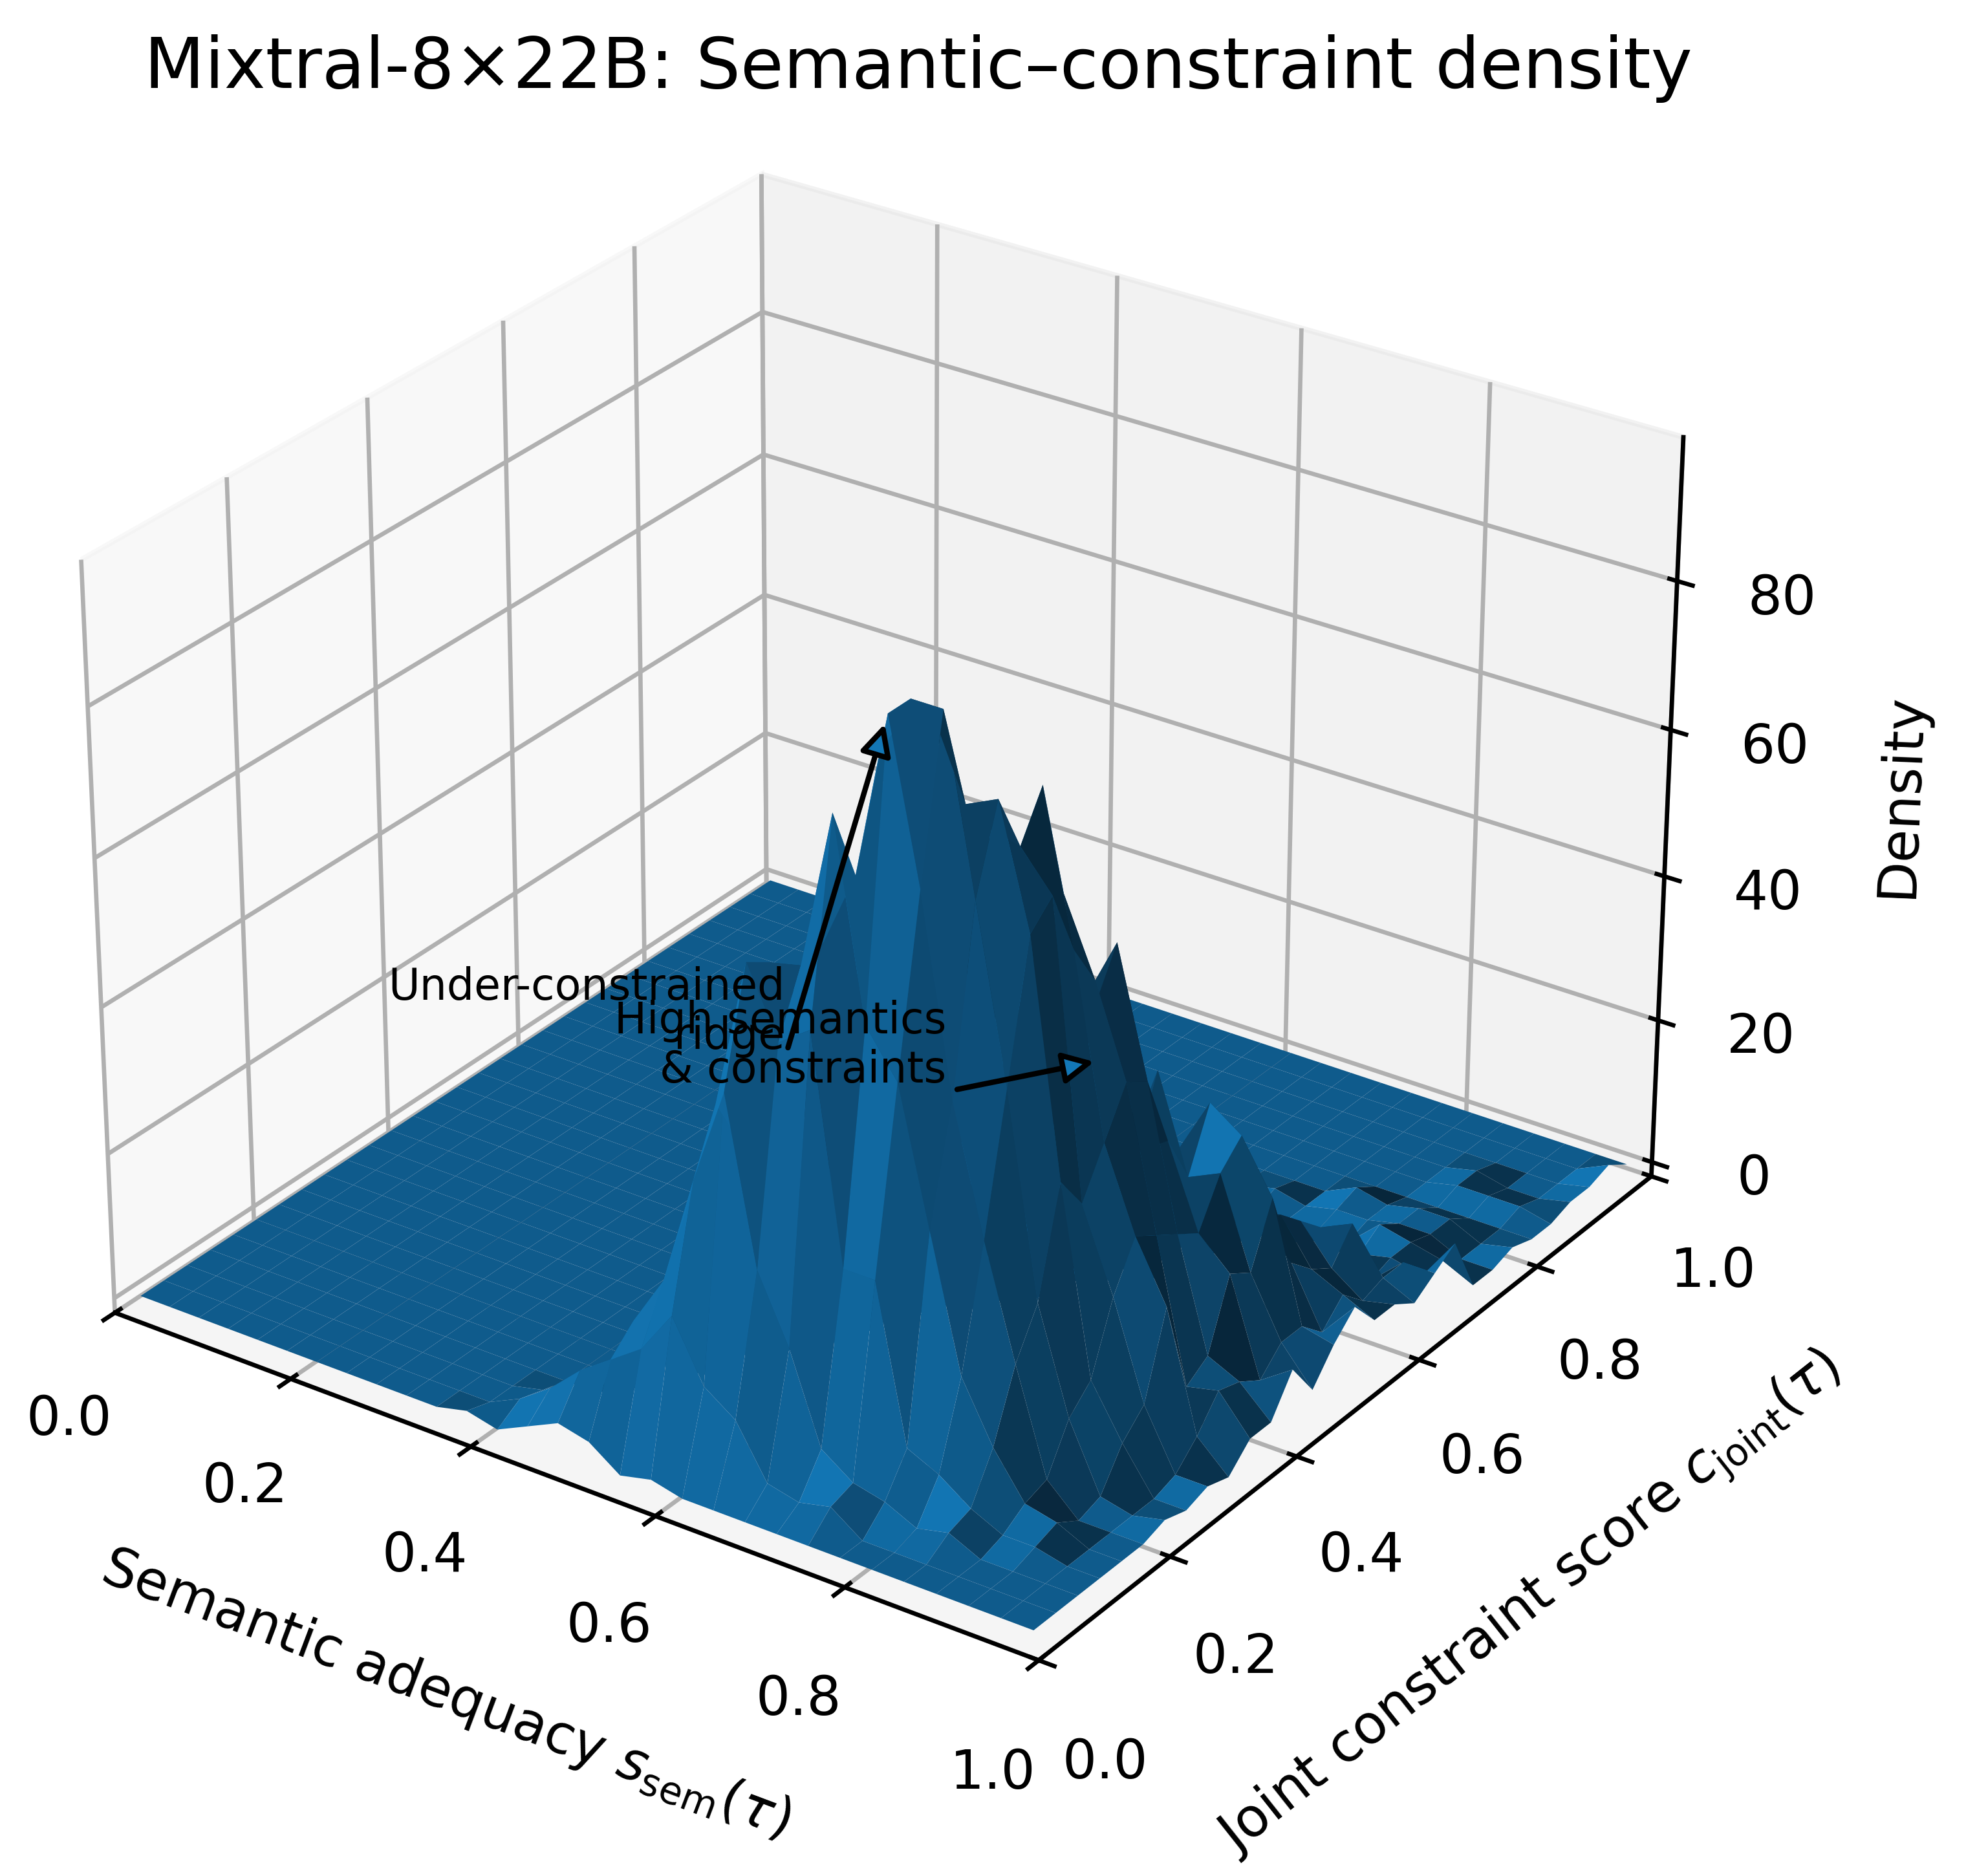
\includegraphics[width=\linewidth]{ICL/instrusum_pareto_surface_mixtral8x22b_annotated.png}
    \subcaption{\textbf{Mixtral--8$\times$22B.}
    The larger Mixtral--8$\times$22B shifts density further toward the
    high--quality corner:
    $s_{\mathrm{sem}}(\tau) \in [0.65, 0.85]$ and
    $c_{\mathrm{joint}}(\tau) \in [0.35, 0.60]$ for most candidates.
    The ridge becomes secondary to a strong peak around $(0.75, 0.55)$,
    showing that the model \emph{naturally places more probability} on
    summaries that respect format, tone, and inclusion.}
    \label{fig:instrusum_semantic_constraint_mixtral8x22b}
  \end{subfigure}

  \vspace{0.6em}

  % (g) Vicuna-7B
  \begin{subfigure}[t]{0.46\textwidth}
    \centering
    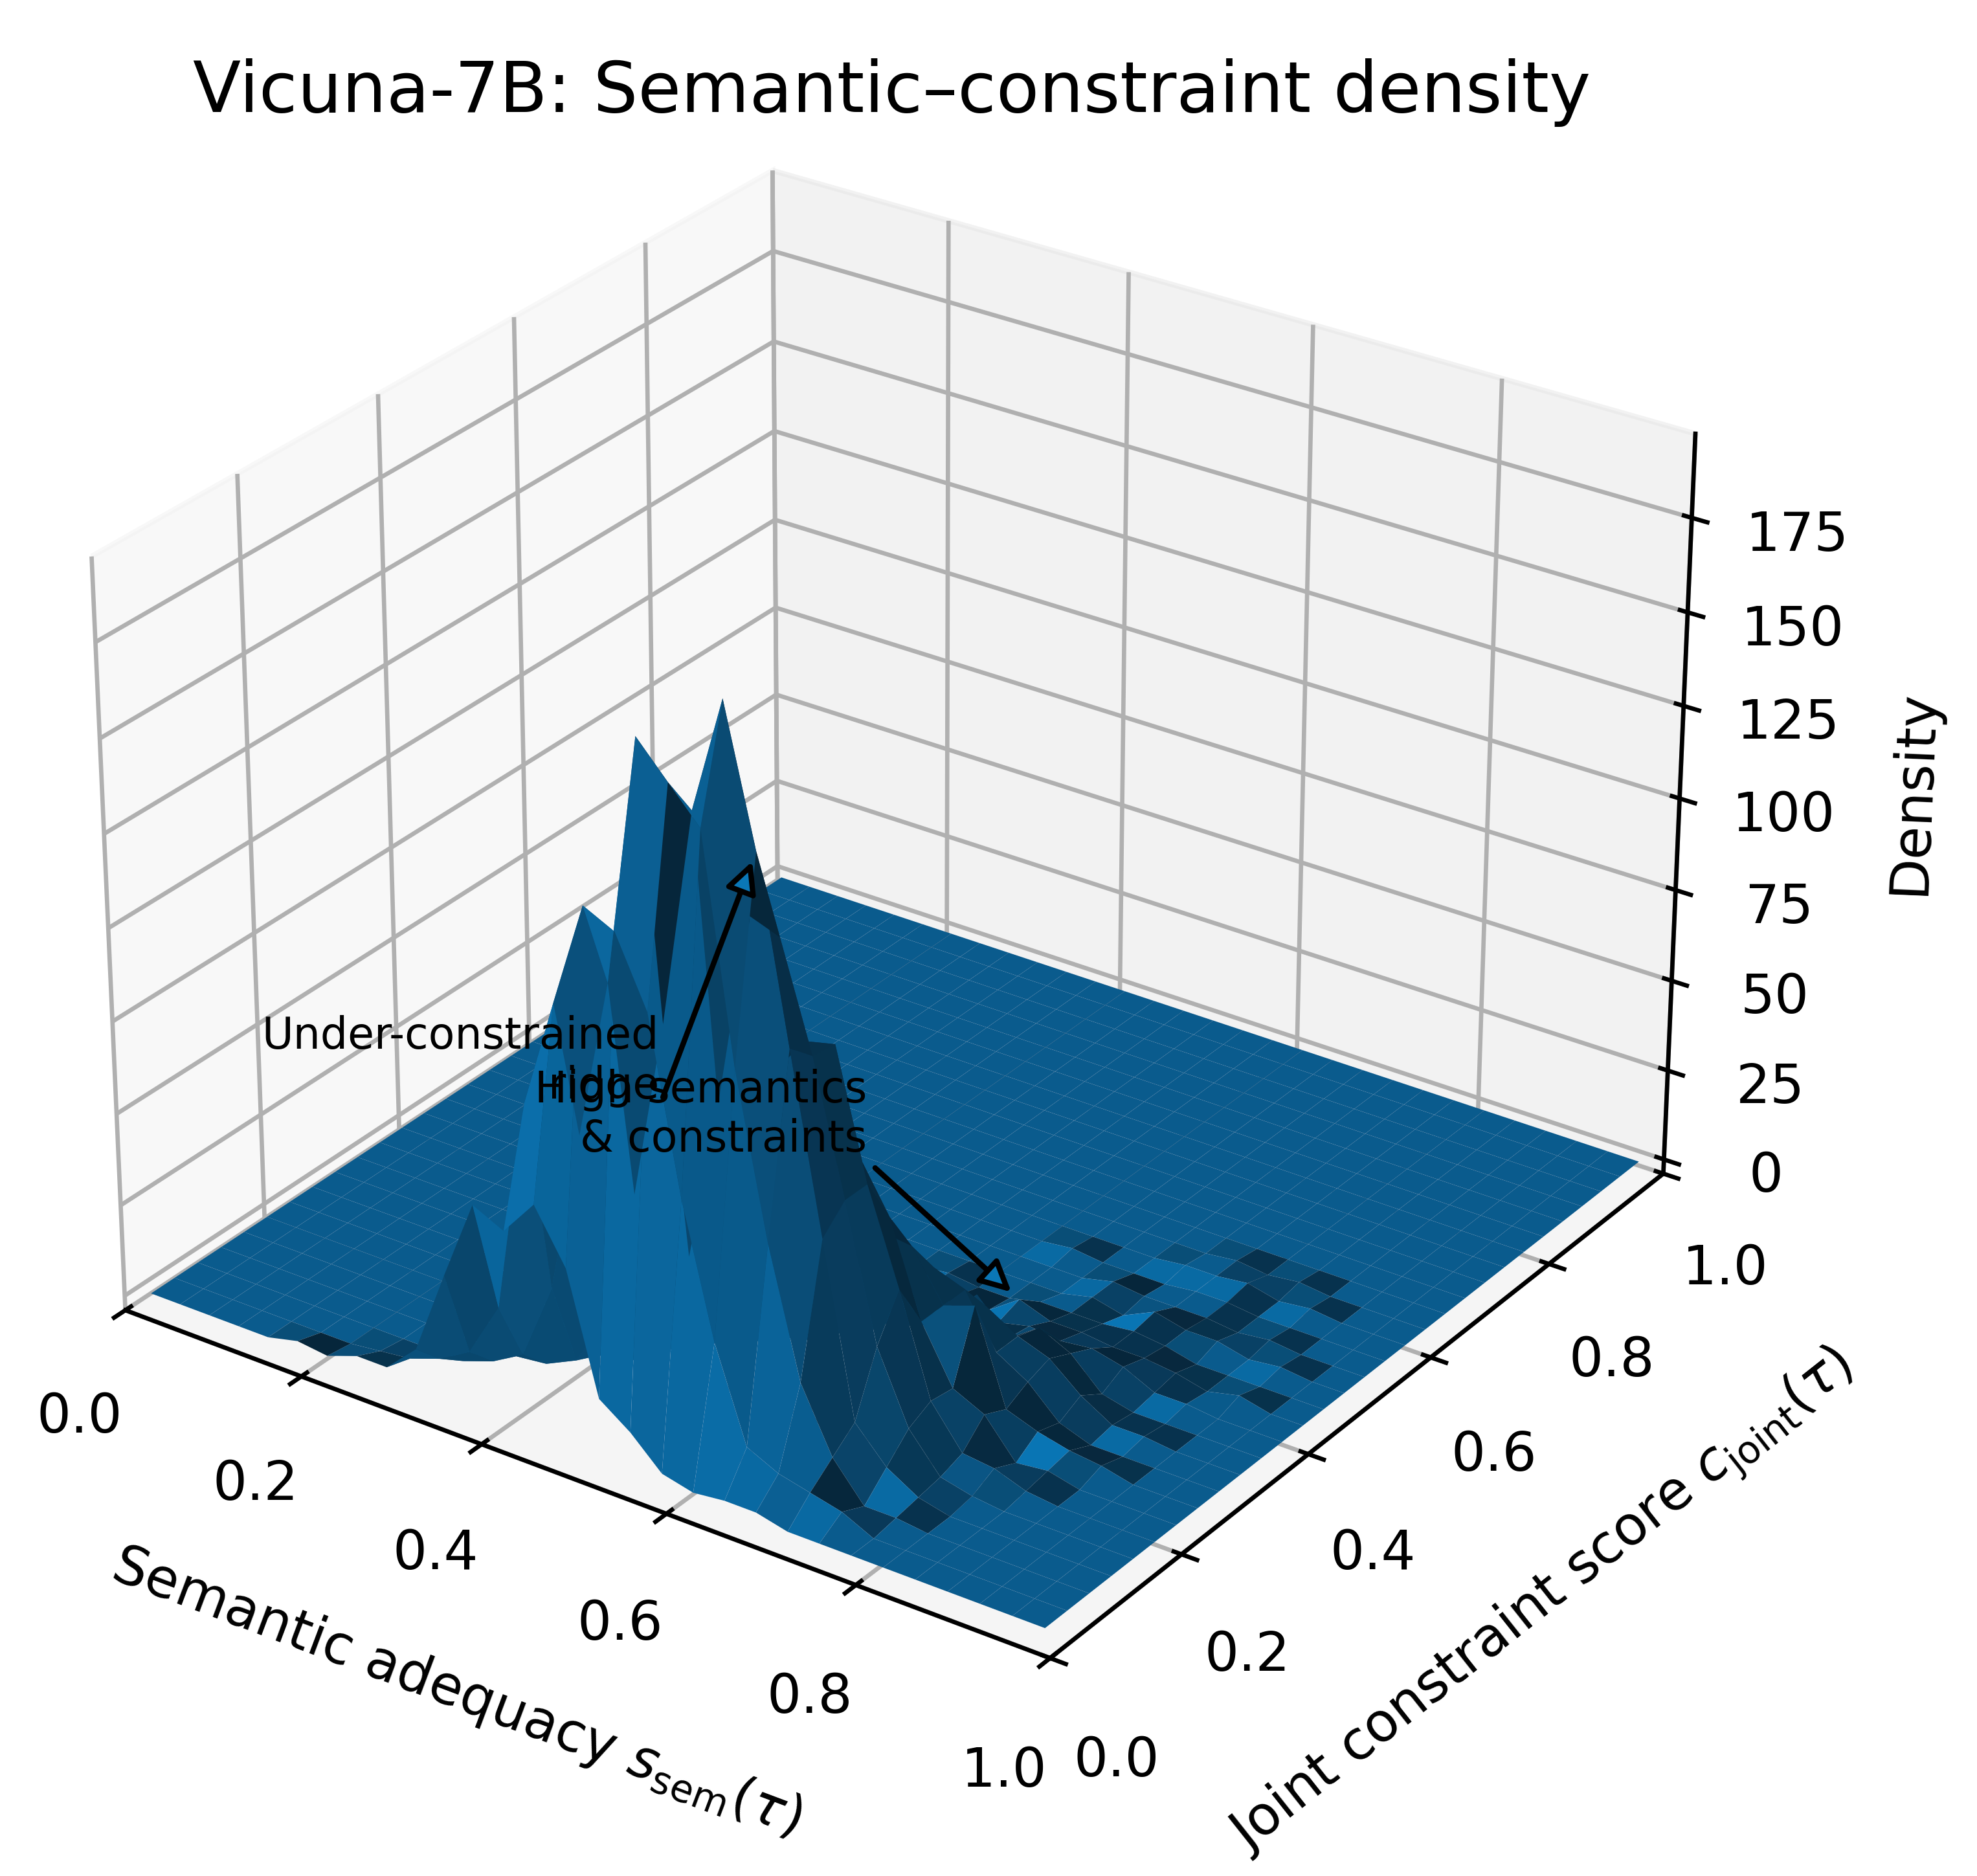
\includegraphics[width=\linewidth]{ICL/instrusum_pareto_surface_vicuna7b_annotated.png}
    \subcaption{\textbf{Vicuna--7B.}
    Vicuna--7B is dominated by a peak in
    $s_{\mathrm{sem}}(\tau) \in [0.50, 0.70]$ and
    $c_{\mathrm{joint}}(\tau) \in [0.10, 0.30]$,
    with little mass beyond $c_{\mathrm{joint}}(\tau) \approx 0.40$.
    The pronounced \emph{under--constrained ridge} reflects a tendency to
    produce semantically competent but stylistically misaligned summaries, while
    the tiny arrowed island of higher $c_{\mathrm{joint}}$ indicates that
    well--aligned candidates exist but sit at the fringes of the distribution.}
    \label{fig:instrusum_semantic_constraint_vicuna7b}
  \end{subfigure}\hfill
  %
  % (h) Phi-2
  \begin{subfigure}[t]{0.46\textwidth}
    \centering
    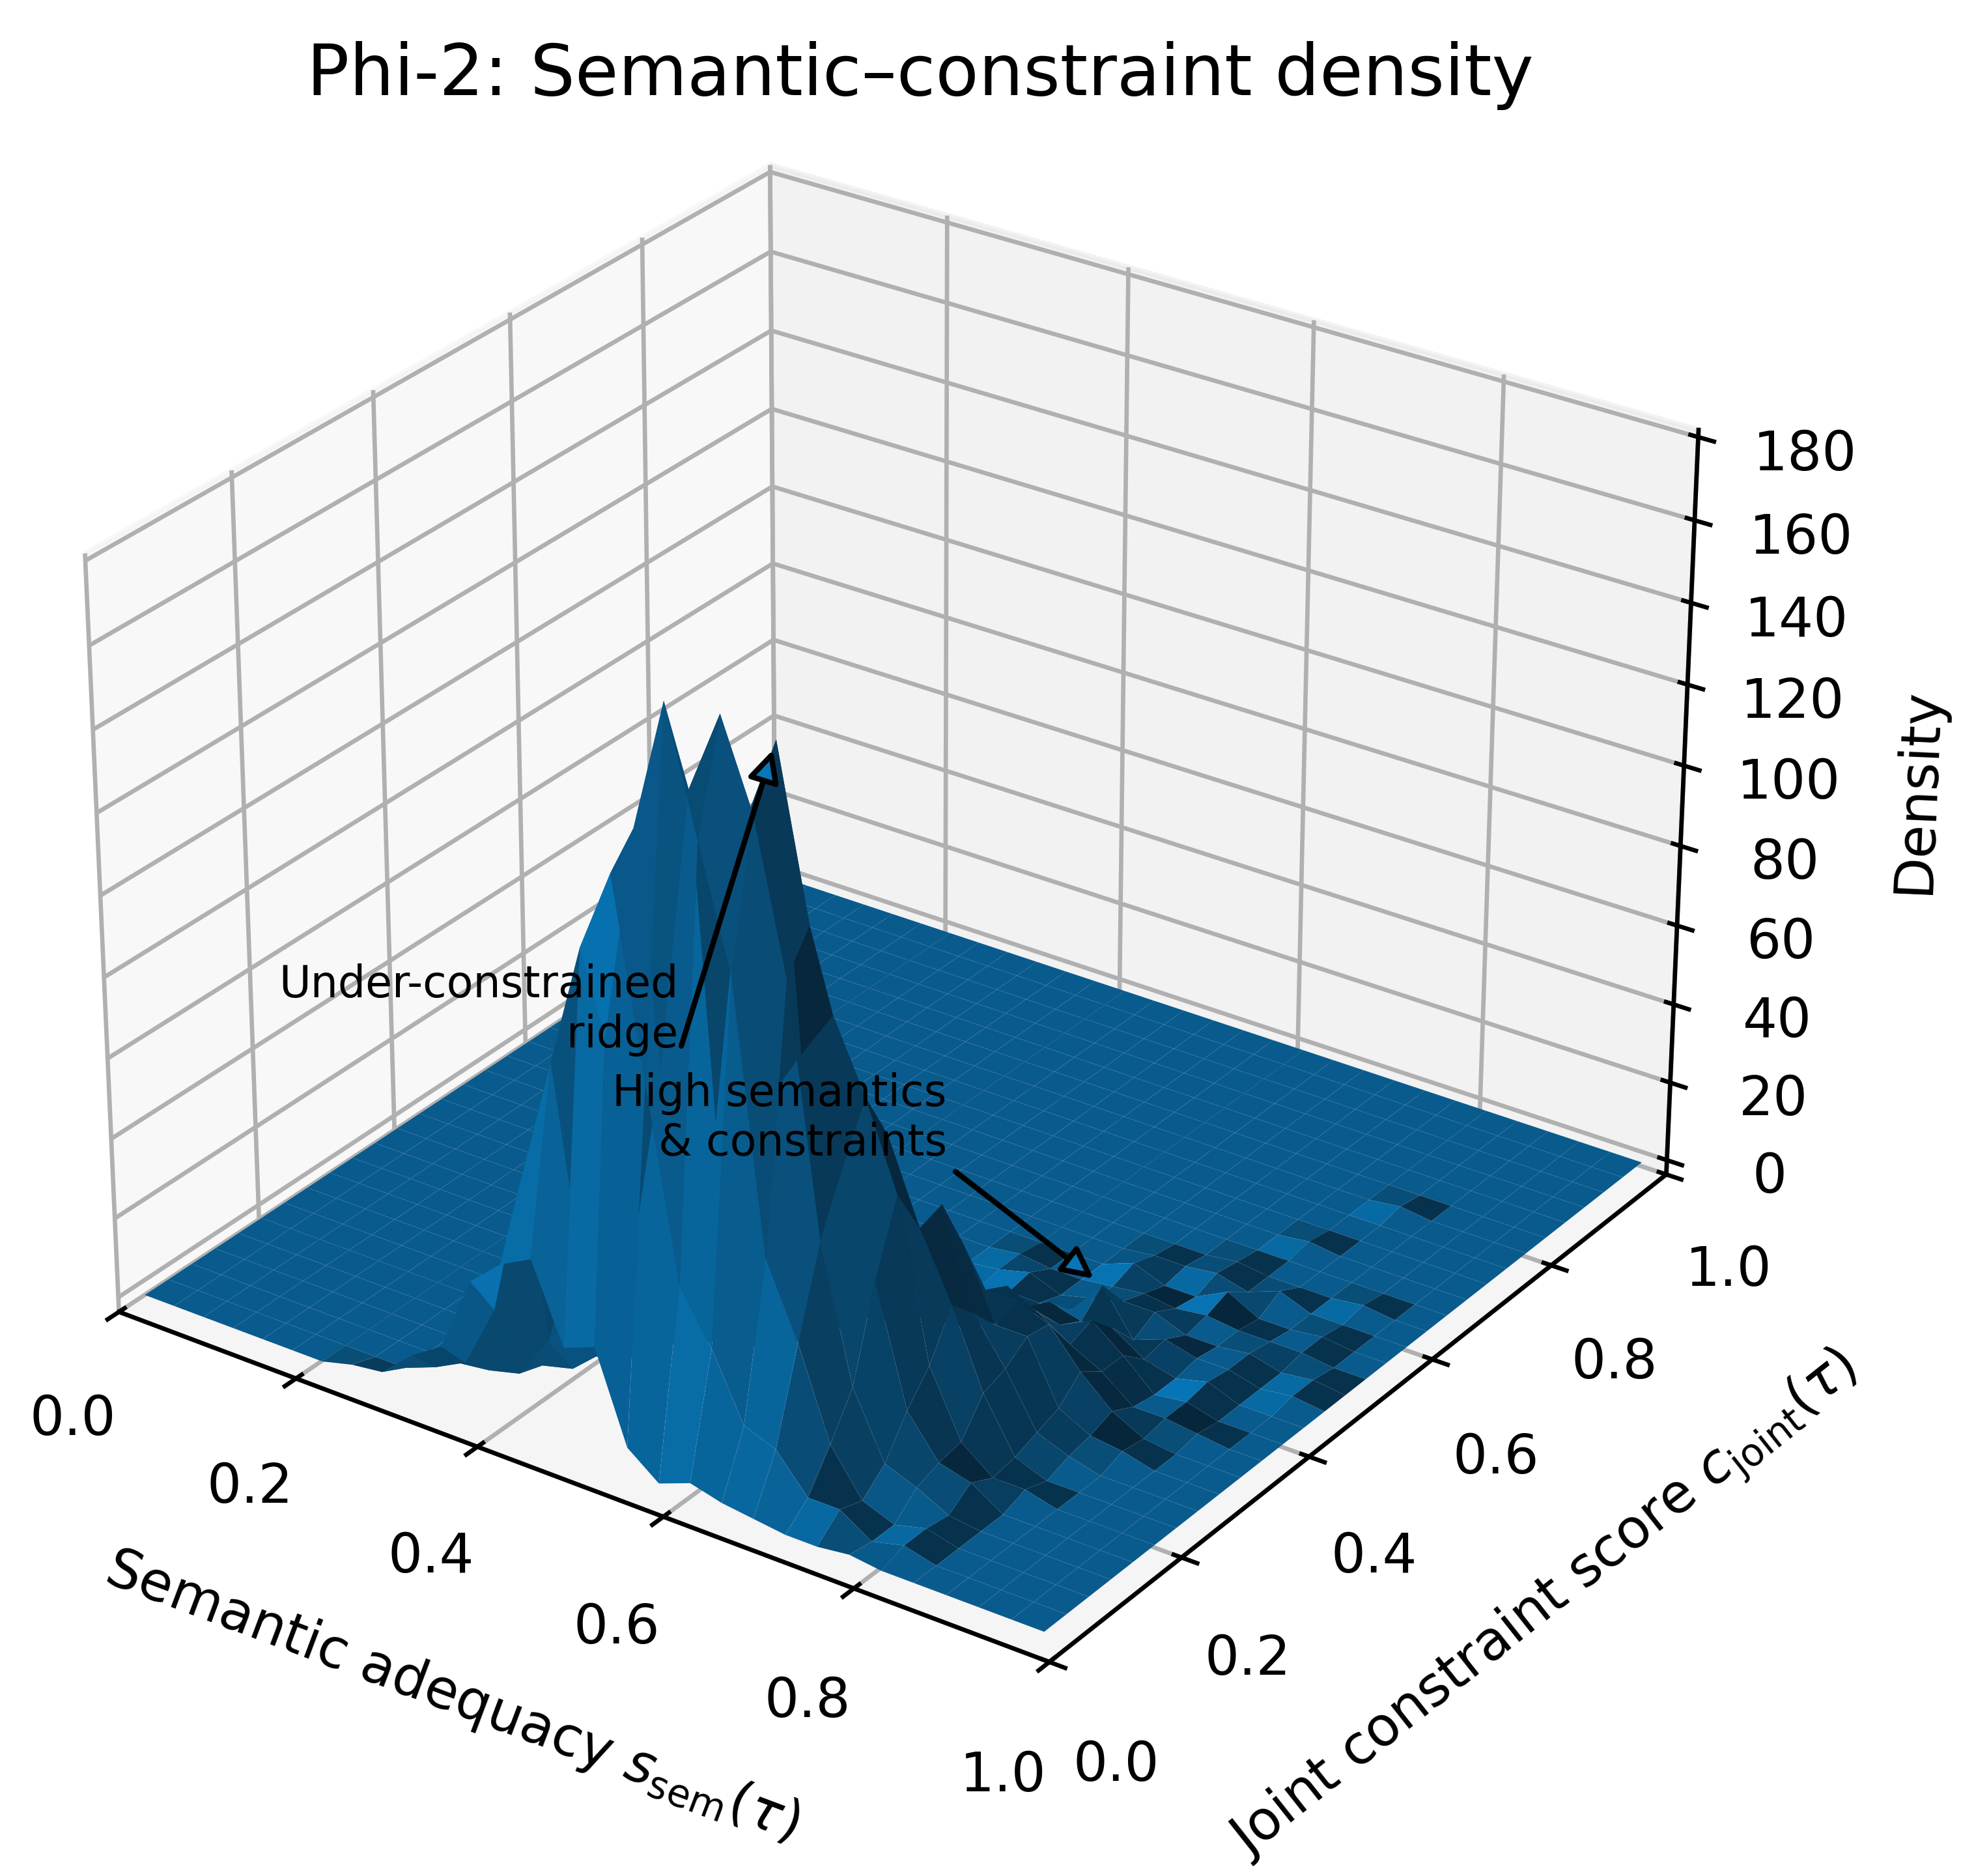
\includegraphics[width=\linewidth]{ICL/instrusum_pareto_surface_phi2_annotated.png}
    \subcaption{\textbf{Phi--2.}
    Phi--2 concentrates mass in
    $s_{\mathrm{sem}}(\tau) \in [0.45, 0.70]$ and
    $c_{\mathrm{joint}}(\tau) \in [0.10, 0.30]$,
    yielding one of the steepest under--constrained ridges.
    The high--constraint region $c_{\mathrm{joint}}(\tau) \gtrsim 0.40$
    is only a \emph{thin, low--density tail}, showing that jointly
    well--aligned summaries are rare and almost never selected by
    deterministic decoding.}
    \label{fig:instrusum_semantic_constraint_phi2}
  \end{subfigure}

  \caption{\textbf{Semantic--constraint density landscapes across models on InstruSum.}
  Taken together, panels \textbf{(a)}--\textbf{(h)} reveal a consistent
  pattern: many instruction--tuned LLMs place most of their probability mass on
  an \textbf{under--constrained ridge} of semantically strong but stylistically
  misaligned summaries, while only a smaller portion of the distribution
  occupies the \textbf{high semantics \& high constraints} region near the
  Pareto frontier.
  As models become larger and more recent (e.g., \textbf{LLaMA--3},
  \textbf{Mixtral--8$\times$22B}), this high--quality corner receives
  increasingly more mass, yet greedy decoding remains anchored to the ridge.
  The figure therefore supports our central takeaway:
  apparent failures to follow detailed style and format instructions are often
  a \emph{search artifact} of the decoding policy rather than a hard limitation
  of the underlying conditional distribution.}
  \label{fig:instrusum_semantic_constraint_all_models}
\end{figure*}




